% Options for packages loaded elsewhere
\PassOptionsToPackage{unicode}{hyperref}
\PassOptionsToPackage{hyphens}{url}
\PassOptionsToPackage{dvipsnames,svgnames,x11names}{xcolor}
\documentclass[
  10pt,
]{article}
\usepackage{xcolor}
\usepackage[margin=2.2cm]{geometry}
\usepackage{amsmath,amssymb}
\setcounter{secnumdepth}{-\maxdimen} % remove section numbering
\usepackage{iftex}
\ifPDFTeX
  \usepackage[T1]{fontenc}
  \usepackage[utf8]{inputenc}
  \usepackage{textcomp} % provide euro and other symbols
\else % if luatex or xetex
  \usepackage{unicode-math} % this also loads fontspec
  \defaultfontfeatures{Scale=MatchLowercase}
  \defaultfontfeatures[\rmfamily]{Ligatures=TeX,Scale=1}
\fi
\usepackage{lmodern}
\ifPDFTeX\else
  % xetex/luatex font selection
\fi
% Use upquote if available, for straight quotes in verbatim environments
\IfFileExists{upquote.sty}{\usepackage{upquote}}{}
\IfFileExists{microtype.sty}{% use microtype if available
  \usepackage[]{microtype}
  \UseMicrotypeSet[protrusion]{basicmath} % disable protrusion for tt fonts
}{}
\makeatletter
\@ifundefined{KOMAClassName}{% if non-KOMA class
  \IfFileExists{parskip.sty}{%
    \usepackage{parskip}
  }{% else
    \setlength{\parindent}{0pt}
    \setlength{\parskip}{6pt plus 2pt minus 1pt}}
}{% if KOMA class
  \KOMAoptions{parskip=half}}
\makeatother
\usepackage{color}
\usepackage{fancyvrb}
\newcommand{\VerbBar}{|}
\newcommand{\VERB}{\Verb[commandchars=\\\{\}]}
\DefineVerbatimEnvironment{Highlighting}{Verbatim}{commandchars=\\\{\}}
% Add ',fontsize=\small' for more characters per line
\newenvironment{Shaded}{}{}
\newcommand{\AlertTok}[1]{\textcolor[rgb]{1.00,0.00,0.00}{\textbf{#1}}}
\newcommand{\AnnotationTok}[1]{\textcolor[rgb]{0.38,0.63,0.69}{\textbf{\textit{#1}}}}
\newcommand{\AttributeTok}[1]{\textcolor[rgb]{0.49,0.56,0.16}{#1}}
\newcommand{\BaseNTok}[1]{\textcolor[rgb]{0.25,0.63,0.44}{#1}}
\newcommand{\BuiltInTok}[1]{\textcolor[rgb]{0.00,0.50,0.00}{#1}}
\newcommand{\CharTok}[1]{\textcolor[rgb]{0.25,0.44,0.63}{#1}}
\newcommand{\CommentTok}[1]{\textcolor[rgb]{0.38,0.63,0.69}{\textit{#1}}}
\newcommand{\CommentVarTok}[1]{\textcolor[rgb]{0.38,0.63,0.69}{\textbf{\textit{#1}}}}
\newcommand{\ConstantTok}[1]{\textcolor[rgb]{0.53,0.00,0.00}{#1}}
\newcommand{\ControlFlowTok}[1]{\textcolor[rgb]{0.00,0.44,0.13}{\textbf{#1}}}
\newcommand{\DataTypeTok}[1]{\textcolor[rgb]{0.56,0.13,0.00}{#1}}
\newcommand{\DecValTok}[1]{\textcolor[rgb]{0.25,0.63,0.44}{#1}}
\newcommand{\DocumentationTok}[1]{\textcolor[rgb]{0.73,0.13,0.13}{\textit{#1}}}
\newcommand{\ErrorTok}[1]{\textcolor[rgb]{1.00,0.00,0.00}{\textbf{#1}}}
\newcommand{\ExtensionTok}[1]{#1}
\newcommand{\FloatTok}[1]{\textcolor[rgb]{0.25,0.63,0.44}{#1}}
\newcommand{\FunctionTok}[1]{\textcolor[rgb]{0.02,0.16,0.49}{#1}}
\newcommand{\ImportTok}[1]{\textcolor[rgb]{0.00,0.50,0.00}{\textbf{#1}}}
\newcommand{\InformationTok}[1]{\textcolor[rgb]{0.38,0.63,0.69}{\textbf{\textit{#1}}}}
\newcommand{\KeywordTok}[1]{\textcolor[rgb]{0.00,0.44,0.13}{\textbf{#1}}}
\newcommand{\NormalTok}[1]{#1}
\newcommand{\OperatorTok}[1]{\textcolor[rgb]{0.40,0.40,0.40}{#1}}
\newcommand{\OtherTok}[1]{\textcolor[rgb]{0.00,0.44,0.13}{#1}}
\newcommand{\PreprocessorTok}[1]{\textcolor[rgb]{0.74,0.48,0.00}{#1}}
\newcommand{\RegionMarkerTok}[1]{#1}
\newcommand{\SpecialCharTok}[1]{\textcolor[rgb]{0.25,0.44,0.63}{#1}}
\newcommand{\SpecialStringTok}[1]{\textcolor[rgb]{0.73,0.40,0.53}{#1}}
\newcommand{\StringTok}[1]{\textcolor[rgb]{0.25,0.44,0.63}{#1}}
\newcommand{\VariableTok}[1]{\textcolor[rgb]{0.10,0.09,0.49}{#1}}
\newcommand{\VerbatimStringTok}[1]{\textcolor[rgb]{0.25,0.44,0.63}{#1}}
\newcommand{\WarningTok}[1]{\textcolor[rgb]{0.38,0.63,0.69}{\textbf{\textit{#1}}}}
\usepackage{longtable,booktabs,array}
\newcounter{none} % for unnumbered tables
\usepackage{calc} % for calculating minipage widths
% Correct order of tables after \paragraph or \subparagraph
\usepackage{etoolbox}
\makeatletter
\patchcmd\longtable{\par}{\if@noskipsec\mbox{}\fi\par}{}{}
\makeatother
% Allow footnotes in longtable head/foot
\IfFileExists{footnotehyper.sty}{\usepackage{footnotehyper}}{\usepackage{footnote}}
\makesavenoteenv{longtable}
\usepackage{graphicx}
\makeatletter
\newsavebox\pandoc@box
\newcommand*\pandocbounded[1]{% scales image to fit in text height/width
  \sbox\pandoc@box{#1}%
  \Gscale@div\@tempa{\textheight}{\dimexpr\ht\pandoc@box+\dp\pandoc@box\relax}%
  \Gscale@div\@tempb{\linewidth}{\wd\pandoc@box}%
  \ifdim\@tempb\p@<\@tempa\p@\let\@tempa\@tempb\fi% select the smaller of both
  \ifdim\@tempa\p@<\p@\scalebox{\@tempa}{\usebox\pandoc@box}%
  \else\usebox{\pandoc@box}%
  \fi%
}
% Set default figure placement to htbp
\def\fps@figure{htbp}
\makeatother
\ifLuaTeX
  \usepackage{luacolor}
  \usepackage[soul]{lua-ul}
\else
  \usepackage{soul}
\fi
\setlength{\emergencystretch}{3em} % prevent overfull lines
\providecommand{\tightlist}{%
  \setlength{\itemsep}{0pt}\setlength{\parskip}{0pt}}
\usepackage{bookmark}
\IfFileExists{xurl.sty}{\usepackage{xurl}}{} % add URL line breaks if available
\urlstyle{same}
\hypersetup{
  colorlinks=true,
  linkcolor={blue},
  filecolor={Maroon},
  citecolor={Blue},
  urlcolor={blue},
  pdfcreator={LaTeX via pandoc}}

\author{}
\date{}

\begin{document}

{
\setcounter{tocdepth}{3}
\tableofcontents
}
\section{Zero Closure Was Four-Dimensional --- Claim Draft
v4}\label{zero-closure-was-four-dimensional-claim-draft-v4}

\subsection{\texorpdfstring{The basic representation is the
four-dimensional \((r,t,R,Q)\), and zero closure imposes on it the light
cone
\(r^2-t^2-R^2-Q^2=0\)}{The basic representation is the four-dimensional (r,t,R,Q), and zero closure imposes on it the light cone r\^{}2-t\^{}2-R\^{}2-Q\^{}2=0}}\label{the-basic-representation-is-the-four-dimensional-rtrq-and-zero-closure-imposes-on-it-the-light-cone-r2-t2-r2-q20}

\textbf{Author:} Noriaki Kihara \textbf{ORCID:} 0009-0004-6753-4020
\textbf{Date:} 12 August 2026 \textbf{Version DOI:}
10.5281/zenodo.21902806 \textbf{Concept DOI:} 10.5281/zenodo.21902805
\textbf{Position:} ``Generative Structure of Dimension'' series ---
Geometry and Algebra of Zero Closure, v4 \textbf{License:} CC BY 4.0

\begin{center}\rule{0.5\linewidth}{0.5pt}\end{center}

Position of this note: \textbf{an interpretive paper}. It contains no
new theorems. It rearranges known theorems under the single closure
condition \(\sum x_n^2 = 0\) and fixes what is determined by it and what
is not. In v3 we measured what actually happens in the numerical model
of the series and compared the geometric statements with the numerical
ones.

\textbf{Changes v1 → v2}: Claim 4 was completely revised. In v1 we said
``zero closure selects centrally symmetric convex configurations'' and
left the assignment of signs for \(N\ge5\) unresolved. In v2 we showed
(a) that the sign is uniquely determined from length data by ``the
dimension of the smallest face containing both endpoints'', and (b) that
for \textbf{parallelotopes} (\(N=2^d\)) the alternating sum vanishes,
and that centrally symmetric plus convex is not enough (the converse
necessity is proved only for \(d=2\); see the v4 corrections). Claim 6B
was newly introduced to show that this strong constraint does not
contradict the ellipsoid structure of Claim 6.

\textbf{Changes v2 → v3}: Claims 10--14, based on measurements of the
numerical model, were added.

\begin{itemize}
\tightlist
\item
  \textbf{Claim 10}: \(\sum x_n^2 = 0\) is an identity that holds only
  in the steady state; it is broken in transient and metastable states.
  We measured this as deviation from the ellipsoidal surface.
\item
  \textbf{Claim 11}: A seed is required for space and matter to be
  generated, and the seed strength directly affects the size of the
  deviation. The seed \(\delta = 0.1\) of this run is large, and the
  deviation persisted even after entry into the metastable state.
  \textbf{Whether the deviation decreases when the seed is weakened or
  when \(\tau\) is extended has not been confirmed.}
\item
  \textbf{Claim 12}: The double-centred readout of the system has at
  most \(N-1\) non-trivial principal axes, and the spectral
  concentration into the top three directions \(A,B,C\) rapidly expands
  the observed scale. The middle directions barely change in magnitude,
  and the lower directions move to the imaginary side. \textbf{Whether
  these can be identified with physical spacetime, or whether another
  map is required, is an open question.} (In v3 we wrote 11 dimensions
  for \(N=12\); in v4 it is 15 for \(N=16\).)
\item
  \textbf{Claim 13}: What is conserved is the \textbf{signed} trace; the
  total real content and the total imaginary content both increase and
  cancel inside the signed sum. This claim explicitly forbids the
  misreading ``a conservation law holds, therefore no expansion
  occurs''.
\item
  \textbf{Claim 14}: Imaginary directions do not appear in the vacuum
  control. They appear together with the generation of matter.
\item
  \textbf{Claim 15}: A quasi-oscillation on the scale of \(10^2\) steps
  is observed, but its period varies as \(\tau\) evolves.
  \textbf{Whether this is due to the second axiom \(U^n = I\) or to some
  other phenomenon is an open question.}
\end{itemize}

The naming of the axes was also changed in v3 (§0B).

\textbf{Changes v3 → v4}: We raised the constraint on the resolution
\(N\) itself to the status of a claim, and replaced the numerical runs
with \(N=16\). We also raised the content of the title's ``four
dimensions'' and the stability of the principal-axis orientation to the
status of claims.

\begin{itemize}
\tightlist
\item
  \textbf{Claim 16}: \textbf{If zero closure is realised as a
  parallelotope family}, the resolution is \(N = 2^d\) (Claim 4-b). This
  note takes \(N = 16 = 2^4\), \(d = 4\). \textbf{This is not a
  sufficient condition} (rank \(= d\) alone is not enough either, and
  satisfying both does not put the vertices on an ellipsoidal surface).
  \textbf{Nor has it been derived that it is a necessary condition for
  all zero-closure solutions} (Claim 4-e).
\item
  \textbf{Claim 17}: If the sign rule is removed, zero closure carries
  no information. With all-real quantities and no signs there is only
  the trivial solution, and if \textbf{both} signs \textbf{and}
  configuration may be chosen freely, non-trivial solutions exist from
  \(N\ge3\) on. \textbf{What selects parallelotopes is the sign rule
  (face dimension), not the form of the equation \(\sum x_n^2=0\).}
\item
  \textbf{Supplement to Claim 4}: We executed the procedure of 4-a
  (lengths \(\to\) configuration \(\to\) convex hull \(\to\) minimal
  face dimension) using lengths alone as input, and confirmed exact
  agreement with the true classification for \(d=2,3,4\) (4-f). We also
  made explicit the exact all-real identity
  \(\sum_{\text{edges}}d^2 = \sum_{\text{main diagonals}}d^2\) and the
  breakdown of which classes become imaginary.
\item
  \textbf{Claim 0}: \textbf{We made explicit, as a claim, the starting
  point that central projection reduces the many-body zero-closure
  problem to a single quadratic equality constraint.} In the real case
  \(\sum x_n^2 = R^2\) represents an arbitrary point \(P\) on the
  surface of a spherical shell, and the constraint reduces to the single
  equation \(X^{\mathsf T}F(X)=0\). That the complex extension
  \(\sum x_n^2 = 0\) can also be written as
  \(x^2+y^2+z^2-t^2 = R^2+Q^2\) was already known, but \textbf{whether
  this preserves the same reduction as an equation representing points
  on a projection surface had not been derived. Under assumptions (S),
  (\(C\) fixed), (U) and (R), we showed that the level set of the three
  visible components at fixed \(C = t^2+R^2+Q^2\) is a closed surface
  (an ellipsoidal surface) defined by a positive-definite quadratic form
  \(G\).} However, what is mathematically required for the right-hand
  side to be conserved is only \(\dot C=0\), and in the component layer
  of this numerical model that can be expected only for steady solutions
  (in transient and metastable states it deviates and oscillates; 0-d).
  \textbf{A conserved quantity does not determine the motion; it only
  determines the space of permitted motions.}
\end{itemize}

\textbf{Corrections within v4 (following third-party review)}: the
following were errors or incomplete derivations and have been corrected.
In every case the modification is \textbf{not to weaken a claim but to
close a hole in the logic}.

\begin{quote}
\textbf{How to read the table (important)}: review was carried out
several times, and \textbf{some corrections were themselves corrected
again by later review}. \textbf{The ``after'' column has been unified to
the content of the final version.} Intermediate proposals have not been
left in place. For example, ``a section at fixed \(t\)'' was corrected
once in that form, but was later re-corrected to ``a section at fixed
\(C=t^2+R^2+Q^2\)''. Similarly ``a sphere under (S)'' was re-corrected
to ``a sphere under (S) + (\(C\) fixed)''.
\end{quote}

{\def\LTcaptype{none} % do not increment counter
\begin{longtable}[]{@{}
  >{\raggedright\arraybackslash}p{(\linewidth - 4\tabcolsep) * \real{0.3333}}
  >{\raggedright\arraybackslash}p{(\linewidth - 4\tabcolsep) * \real{0.3333}}
  >{\raggedright\arraybackslash}p{(\linewidth - 4\tabcolsep) * \real{0.3333}}@{}}
\toprule\noalign{}
\begin{minipage}[b]{\linewidth}\raggedright
Location
\end{minipage} & \begin{minipage}[b]{\linewidth}\raggedright
Before
\end{minipage} & \begin{minipage}[b]{\linewidth}\raggedright
After
\end{minipage} \\
\midrule\noalign{}
\endhead
\bottomrule\noalign{}
\endlastfoot
Claim 6 & The vertices lie on an ellipsoid \textbf{only if}
\(n\le d(d+1)/2\) & \textbf{Wrong. Counterexamples in both directions}
(one of them is Claim 6B itself). Demoted to a rule of thumb for
over-determination \\
Claim 15, §3B & If \(U^n=I\) then \textbf{there are no fixed points} &
\textbf{Wrong.} \(U=I\) is a counterexample. The period divides \(n\)
(including period 1) \\
Claim 0-c & It appears as an ellipsoidal surface because the readout is
not isotropic & \textbf{Not a derivation.} The readout map
\(X=\Lambda u\) is made explicit and the result derived from
\(G=(\Lambda^{-1})^{\mathsf T}\Lambda^{-1}>0\). It is also made explicit
that this is \textbf{the level set of the three visible components at
fixed \(C=t^2+R^2+Q^2\)} \\
Claim 0 title & A conserved quantity \textbf{determines the motion} & A
conserved quantity \textbf{determines the space of permitted motions} \\
Claim 18-e & Non-decay of the deviation \textbf{follows} from the
conserved quantity & \textbf{This contradicted Claim 0.} Non-decay is a
measured fact, not a derived consequence \\
Claim 4 title, 16-a & Zero-closing configurations \textbf{are}
parallelotopes & Necessity for \(d\ge3\) is unproved (4-e). Restricted
to \textbf{the condition for realisation as a parallelotope family} \\
Claim 17-b & If signs are free it is \textbf{always solvable} & False
for a fixed distance set (the equilateral triangle is a counterexample).
Restricted to the case where \textbf{both signs and configuration} are
free \\
Claim 5 & Zero closure \textbf{fixes} \(\mathrm{tr}(T)\) & By
homogeneity the absolute value is not determined. \textbf{What is
imposed is the single signed condition \(S(D)=0\); the unsigned
\(U(D)=N\mathrm{tr}(B)\) is not determined} (re-corrected in a later
round) \\
Claim 8 & \(\sum q_np_n\) is a generator, \textbf{equivalent} to the
meaninglessness of the overall scale & No symplectic structure has been
introduced. Replaced by \textbf{the cone argument from homogeneity}
(which is more rigorous) \\
Claim 9 & Compactness \textbf{hence} a discrete spectrum & An operator
must be specified. Restricted to \textbf{compactness alone} \\
Claim 2 & The unit is two-dimensional because the relation is two-body &
Made explicit that the map ``edge \(\to\) two-dimensional state unit''
is \textbf{not given} \\
Notation & The \(T\) of \((r,T,R,Q)\) collided with the inertia tensor
\(T\) & The base-layer degree of freedom was changed to lower-case
\(t\) \\
Claim 0-b & There is \textbf{one} constraint & For general complex
numbers there are \textbf{two} (equality plus orthogonality).
\textbf{Only under assumption (S: separation of the supports of the real
and imaginary parts) does it reduce to one.} (S) is the content of Claim
7 but does not hold in the numerical model \\
Claim 0-b & \(\sum_n x_n^2\) was written as both \(0\) and
\(t^2+R^2+Q^2\) & The index ranges differ. Organised with the
\(\mathcal{I}_\pm\) split as
\(\sum_{n\in \mathcal{I}_+}x_n^2 = t^2+R^2+Q^2\) \\
Claim 0-c & The reduction \(\mathbb{R}^M \to \mathbb{R}^3\) was
performed silently & A general linear surjection maps a sphere to a
\textbf{solid ellipsoid}. Made explicit that restriction to a
three-dimensional subspace \(U\) is required first, and decomposed the
underived part into three stages \\
Claim 0-c′ & \(\frac{d}{d\tau}(X^{\mathsf T}GX) = 0\) & This
contradicted 0-d.~The correct form is \(= \dot C\). \(\dot G\) (shape
and orientation), \(\dot C\) (scale) and \(\dot X\) (motion on the
surface) separate \\
Claim 0-c′ & Diffusion of the orientation is \textbf{direct evidence}
that \(G\) is not fixed & It presupposes identifying the eigendirections
of \(G\) with the top three principal axes. Since that identification is
itself unresolved, the statement is \textbf{conditional} \\
Notational remark in Claim 5 & \(T\) and \(B\) ``coincide when \(B\) is
positive semi-definite'' & \textbf{They cannot coincide, since the
matrices have different sizes.} \(B = VV^{\mathsf T}\) (\(N\times N\)),
\(T = V^{\mathsf T}V\) (\(d\times d\)); the non-zero eigenvalues agree
with multiplicity and \(\mathrm{tr}(B)=\mathrm{tr}(T)\) \\
Body of Claim 8 & Scale symmetry follows from the \textbf{complex
convention} & It does not depend on complexity. It follows from
\textbf{the equation being homogeneous} (the conclusion had been
corrected but the body had not) \\
§3 & ``Dynamics, time evolution and interaction have not been measured''
& \textbf{Wrong.} Claims 10--18 measure time evolution extensively. The
correct statement is ``\textbf{the dynamical law \(F\) has not been
derived}'' \\
Claim 0-c & ``Unconditionally: the section at fixed \(t\) is a sphere''
& \textbf{Not unconditional.} No assumption \(\to\) two constraints /
(S) \(\to\) one equality constraint (a \textbf{family} of spheres) / (S)
+ (\(C\) fixed) \(\to\) \(S^{|\mathcal{I}_+|-1}\) / + (U) \(\to\)
\(S^2\) / + (R) \(\to\) ellipsoidal surface: organised into \textbf{five
stages}. What must be fixed is not \(t\) but \(C=t^2+R^2+Q^2\) \\
Claim 0-b & \(\sum_n x_n^2 = t^2+R^2+Q^2\) reappeared immediately after
the \(\mathcal{I}_\pm\) split & Unified to
\(\sum_{n\in \mathcal{I}_+}x_n^2\). Also made explicit that the form
\(x^2+y^2+z^2-t^2\) presupposes the choice of ``three visible
components'' and therefore belongs after assumption (U) \\
Claim 5 & ``The constraint is one condition'' in general & \textbf{This
clashed with Claim 0-b.} For general complex numbers there are two.
Restricted to \textbf{the layer of real distance geometry}, and to
statements under assumption (S) \\
Claim 0-c′ & \(\dot G\) = shape, \(\dot C\) = scale & Not unique because
of the redundancy \(G\mapsto\alpha G,\ C\mapsto\alpha C\). Made unique
by \(G = g\widehat G\), \(\det\widehat G=1\), \(\rho^2 = C/g\) \\
Heading of 4-d, 6B, 16-b & Parallelotopes are ``necessary'',
``required'', ``the only ones that lie on it'' & Necessity is unproved
for \(d\ge3\). Changed to ``a stronger constructive family exists'',
``which Claim 4-b guarantees'', ``in this test only parallelotopes gave
1, but uniqueness is unproved'' \\
Claim 8 title & Scale symmetry is not an independent axiom
(unconditional) & Distinguished \textbf{reading A (invariance of the
solution set) and reading B (identification of states)} of axiom 0.5.
Under A it can be dropped; under B a projectivisation is separately
required. Deciding which is intended is an open task \\
Claim 1 & ``The motion of the system decomposes into a direct sum of
two-dimensional rotation planes'' & The decomposition is \textbf{per
generator}, and since the algebra is non-commutative different
generators cannot be block-diagonalised simultaneously. The rank is the
dimension of a maximal abelian subalgebra, not a permanent number of
units \\
Claim 2B & The explanation of four dimensions had become excessively
conditional & \textbf{Returned to the skeleton.} The basic
representation is the \textbf{four-dimensional} \((r,t,R,Q)\), and zero
closure imposes on it the \textbf{light cone} \(r^2-t^2-R^2-Q^2=0\).
That is enough. \(x,y,z\) belong to the later three-dimensional readout,
and the Stiefel manifold, the product of spheres and the number of
hidden components are not needed for the four-dimension claim \\
Claim 0-c & \(\mathbb{R}^M\), \(S^{M-1}\), \(U\subset\mathbb{R}^M\) in
the reduction argument & After (S) the object is the \textbf{visible
side}. Unified to \(\mathbb{R}^{|\mathcal{I}_+|}\),
\(S^{|\mathcal{I}_+|-1}\), \(U\subset\mathbb{R}^{|\mathcal{I}_+|}\) \\
Claim 0 title & ``This reduction is not lost under complex extension''
(unconditional) & For general complex numbers there are two constraints.
\textbf{``Under assumption (S)''} was added \\
End of 0-c, Claim 2B & Jumped directly to \(S(D)=0\) & Made explicit
that assumption (\(\Gamma\)) is used \\
Claim 0-c′ & A varying \(C\) was called a \textbf{conserved quantity} &
Do not call something conserved when it is not. Unified to ``the
quadratic scale \(C\)'', reserving ``conserved quantity'' for the case
\(\dot C=0\). ``\(\dot C=0\) only in the steady state'' was also changed
to ``\textbf{what can be expected to persist over an interval is}'',
since it can occur at isolated times \\
Claim 0-b & The Stiefel 2-plane as ``a partial answer to the
two-dimensionality of Claims 1 and 2'' & \textbf{The three ``2''s live
in different spaces.} Stiefel is in the relation-coefficient space
\(\mathbb{R}^M\), Claim 1 is in the vertex space \(\mathbb{R}^N\), Claim
2 is an abstract state unit. The identifying map is underived \\
Claim 0-c & The full state set under (S) written as
\(\bigcup_C S^{|\mathcal{I}_+|-1}\) & \textbf{It is a product of
spheres.} At fixed \(C\) the full state set is
\(S^{|\mathcal{I}_+|-1}\times S^{|\mathcal{I}_-|-1}\); the projection to
the visible side is the family of spheres. If all \(C\) are allowed, the
union on the visible side is all of \(\mathbb{R}^{|\mathcal{I}_+|}\) and
no information remains \\
Claim 0-b & ``In the model there are still two constraints'' connected
to the three quantities measured in 18-b & Different questions. The
former is the number of target conditions in the component layer; the
latter is which quadratic quantities are conserved in the readout layer.
\(\sum_e x_e^2\) is non-zero in the readout layer \\
§6 tasks & Assumption (\(\Gamma\): geometric sign correspondence) was
missing & Restored to five items. The agreement of the
\(\mathcal{I}_\pm\) split with the face-dimension sign is
\textbf{exactly the gap of §3B}; without it complex zero closure and
\(S(D)=0\) are not connected \\
Claim 18-f & The \(\delta\) sweep \textbf{can discriminate} option 1
from 2 and 3 & \textbf{Logically wrong.} Even if the diffusion stops, 1
cannot be denied. What can be measured is only whether the diffusion is
transient/seed-dependent or persists in the steady limit. An experiment
discriminating the three readings has not been designed \\
Notation & \(L\) (index set and readout map), \(R\) (index set and
physical quantity), \(G\) (assumption and positive-definite matrix)
collided & Index sets renamed to \(\mathcal{I}_\pm\), the readout map to
\(\Lambda\), and the geometric-sign assumption to (\(\Gamma\)) \\
Claim 2B & The \(\lambda\) of the projectivisation
\(\sim\lambda(r,t,R,Q)\) was unrestricted & \(r\) is a length with
\(r\ge0\), so \(\lambda>0\). To include signs, introduce
\(\tilde r\in\mathbb{R}\) and set \(r=|\tilde r|\) \\
Claim 14 & Vacuum rank 15 described as ``\textbf{that is, no
degeneracy}'' & \textbf{The opposite.} Rank 15 only says that the 15
non-trivial eigenvalues are non-zero. In fact they are all \(0.0645\),
i.e.~\textbf{maximally degenerate}. Changed to ``the 15 eigenvalues
other than the trivial zero are non-zero; in the late regime the
spectrum is completely degenerate and isotropic'' \\
Claim 14 & The negative eigenvalues of \(B\) \textbf{identified with the
imaginary symbol} of Claim 7 & This re-connected the three layers
separated in Claim 5 (real/imaginary of the complex form, face-dimension
sign, sign of the eigenvalues of \(B\)). Changed to ``the identifying
map is underived; it remains a qualitative candidate correspondence'' \\
End of Claim 10 & ``The scope of Claims 1--9 \textbf{is limited to the
steady state}'' & Claims 4 and 6B are static geometric theorems and do
not require stationarity. Changed to ``the propositions themselves do
not require the steady state; to apply them to this model the premises
must hold, and in transient and metastable states they do not'' \\
Claim 13 & ``The structure is the same when \(N\) is changed'' & Only
two points were checked. By the same standard as Claim 12, changed to
``\(N\)-independence is underived'' \\
Claim 14 & Asserted the \textbf{cause} of the larger vacuum deviation at
\(N=16\) & Not a comparison under identical conditions. Changed to
``qualitatively consistent with the trend of Claim 16-b; the cause has
not been established'' \\
Claim 9 & The real spinor square map is ``2:1'' & 2:1 \textbf{away from
the origin} (the preimage of the origin is a single point). In the
projectivisation the origin is removed, so this causes no problem \\
§5.4 heading & ``What are the 15 \textbf{dimensions}'' & The measured
rank is 8--11. Changed to ``what are the 15 \textbf{principal axes}''
(because ``15 dimensions'' reads as configuration dimension 15) \\
Claim 12 & ``If the rank falls to \(d=4\) then \textbf{a parallelotope
has been reached}'' & \textbf{Wrong.} It contradicts the counterexample
of Claim 16-b (a random configuration with \(N=16\), rank \(=4\) is
neither a parallelotope nor on an ellipsoidal surface). Changed to ``a
four-dimensional parallelotope must have rank 4; the measured rank is
8--11, so it is not a parallelotope. The converse, however, does not
hold'' \\
Claim 18-e & The non-zero constant of the readout layer described as
``\textbf{zero closure} is not broken'' & Zero closure is defined as
\(\sum x_n^2=0\). The readout-layer \(\sum_e x_e^2\) is
\textbf{non-zero}, hence not zero closure. Changed to ``it exists as a
non-zero conserved quantity'' \\
Claim 0-d & ``State in which layer 0-c is being used'' & \textbf{Neither
layer satisfies all the assumptions of 0-c} (the component layer has
varying \(C\); the readout layer fails (S)). Changed to ``it is
necessary to establish in which layer and under which map (S), (U) and
(R) hold'' \\
Claim 0-d & ``The `solvability' of 0-c is a statement \textbf{about the
steady state}'' & 0-c does not require stationarity, only \(\dot C=0\).
The steady state is needed because in the component layer of this model
\(C\) can be expected to be fixed only for steady solutions \\
Claim 18 title & ``What is conserved is an \textbf{inner product}'' &
\(\sum x_e^2\) is a quadratic form built from a complex symmetric
bilinear form, not an inner product. Changed to
``orientation-independent \textbf{quadratic forms} are conserved'' \\
Heading of 18-b & ``There are \textbf{two}'' conserved quantities & It
has not been shown that there are no others. Changed to ``\textbf{at
least two kinds} are confirmed'' \\
§6 Question 1 & The complex representation ``saves one axiom'' & What
reduces the axiom is \textbf{the homogeneity of the zero-closure
equation}, not the complex representation. What the complex
representation adds is the orthogonality condition \(\sum q_np_n=0\) \\
Misreading 3, Claim 12 & ``This is not compactification'' & What the
numbers can deny is the \textbf{shrinking} picture. Restricted to ``it
is not compactification of the type in which extra directions shrink and
become invisible'' \\
Claims 6, 2B and Figure 4 & ``Zero closure constrains \(l=0\) (the
magnitude)'' & \textbf{A chain that became wrong through the correction
to Claim 5.} Zero closure \(S(D)=0\) does not fix the scale (for the
parallelotope family it is an identity, so it holds under any choice of
generators). What determines \(l=0\) is \textbf{fixing \(C\) or a
normalisation} \\
Claim 5 title & ``What is constrained is one \textbf{trace-type}
condition'' & \(S(D)=0\) is not a trace-type condition. Changed to ``it
imposes the single signed condition \(S(D)=0\); the unsigned
\(U(D)=N\mathrm{tr}(B)\) is not determined by zero closure alone'' \\
Claim 5 & Written as if the face-dimension sign rule followed from
assumption (S) & \textbf{Assumption (\(\Gamma\): geometric sign
correspondence) is separately required.} (S) gives only the separation
of supports; it does not give \(\mathcal{I}_+=\{s_e=+1\}\),
\(\mathcal{I}_-=\{s_e=-1\}\). This is exactly the gap of §3B \\
Claim 7 & The group generated by \(i\) is \(\mathbb{Z}_2\) & \textbf{At
the amplitude level it is \(\mathbb{Z}_4\)} (\(1\to i\to-1\to-i\to1\)).
What becomes \(\mathbb{Z}_2\) is the induced action on the sign of the
squared quantity \\
Claim 12 title & ``The system has \(N-1\) \textbf{degrees of freedom}''
& Not degrees of freedom, but \textbf{at most \(N-1\) non-trivial
principal axes (signed spectral directions)}. The same reason as the
distinction between ambient dimension and independent degrees of freedom
in Claim 2B \\
Claim 5 & From the unsigned identity \(\sum d^2=N\mathrm{tr}(B)\) to
``zero closure constrains one trace-type condition'' & \textbf{Confusion
of the signed \(S(D)=\sum s_ed_e^2\) with the unsigned
\(U(D)=\sum d_e^2\).} \(S(D)=0\) does not determine the value of
\(U(D)\). Only with \(C\) fixed do we obtain \(U(D)=2C\) and
\(\mathrm{tr}(B)=2C/N\). The ``sign of the eigenvalues of \(B\)'' in
Claim 13 is a third, different thing \\
Claims 4-b and 6B & The generators were written \(u_i\) in both sections
& \textbf{A factor-2 discrepancy} (factor 2 in edge length, factor 4 in
\(\Sigma d^2\); verified numerically). 4-b uses edge vectors \(e_i\); 6B
uses \(A\equiv\frac12[e_1\cdots e_d]\) \\
Claim 0-c & ``Fix \((t,R,Q)\), \textbf{equivalently} fix \(C\)'' &
\textbf{Not equivalent.} Even with \(C\) constant, \((t,R,Q)\) can be
redistributed. What is required is fixing \(C\); fixing \((t,R,Q)\)
individually is a stronger sufficient condition. Also
``three-dimensional section'' is inaccurate; the correct phrase is
``\textbf{the level set of the three visible components at fixed
\(C\)}'' \\
Claim 2 & ``The number of common components is 3'' asserted immediately
before stating that the aggregation rule is underived & Separated into
three layers: 3 for a single block (proved) / 3 for the whole system
(numerical fact) / the aggregation rule connecting them (underived) \\
Claim 0-c & Assumption (R) had swallowed (U) & Separately defined (U:
the state lies in a three-dimensional subspace) and (R:
\(\Lambda:U\to\mathbb{R}^3\) is linear and regular) \\
Claim 6 & ``Saturation is caused by the closure condition being
quadratic'' & \textbf{Not accurate.} The cause is that the readout is
the second-order tensor \(T\). Fourth moments do distinguish the cases
(the numerical checks in the text show this) \\
Claim 6 & \(l=2\) is ``shape 2 + orientation 3'' & The 5 components are
always correct, but that decomposition holds \textbf{in the
non-degenerate generic case}. At degeneracies the eigendirections lose
meaning \\
Claim 4-a & ``Splits into exactly \(d\) classes'' & For a general
polytope some classes may be empty (a simplex has only \(k=1\)). Changed
to ``each pair is assigned a unique \(k\); for parallelotopes all
classes appear'' \\
§3B & The numerical model ``\textbf{imposes}'' \(\sum x_e^2=0\) & A hard
constraint could not be broken. In fact it is non-zero (Claim 10).
Changed to ``\textbf{it is placed as a steady-state closure condition};
it is not enforced by projection at each step'' \\
Claim 0-c & ``Under assumption (S): the visible side is a sphere
\(S^{|\mathcal{I}_+|-1}\)'' & \textbf{(S) alone does not give a sphere.}
\(C\) can vary, so the permitted states form a family (cone) of spheres
\(\bigcup_C S^{|\mathcal{I}_+|-1}_{\sqrt C}\). It becomes a sphere only
when (\(C\) fixed) is added. Four stages \(\to\) \textbf{five stages} \\
Claim 6 & The multipole table contained \(l=1\) (centre offset, zero by
central symmetry) & \textbf{Wrong twice.} \(l=1\) is the first moment
and is not a component of \(T\) (the decomposition of \(\mathrm{Sym}^2\)
is \(l=0\oplus l=2\) only). Moreover it vanishes not by central symmetry
but \textbf{by the definition of barycentric coordinates} \\
Opening of 6B & ``The circumscribed ellipsoid and the inertia ellipsoid
are identical'' & Unified to identical with the \textbf{normalised}
inertia ellipsoid (\(c=d/N\)) (the conclusion had been corrected but the
opening had not) \\
Claim 6B & ``A parallelotope is \textbf{not a generic configuration}'' &
The word can be read either way. Changed to ``\textbf{it is not a
configuration in general position}; the vertices are built from \(d\)
generators, so there are dependencies among the conditions'' \\
Claim 17-b & With free signs and configuration it is ``\textbf{almost
always}'' satisfiable & A measure-theoretic statement, unproved. Deleted
and replaced by ``a non-trivial family of configurations exists; hence
the zero-closure equation alone cannot select uniquely'' \\
Claim 3 title & ``The only thing undetermined is the \textbf{sign of the
signed volume}'' & For degenerate configurations the volume is \(0\) and
the binary choice does not exist. Changed to ``\textbf{for a
non-degenerate maximal-dimensional configuration}, the only thing
undetermined is the \(\mathbb{Z}_2\) of orientation (reflection)'' \\
Claim 0 title and text & ``Reduces to motion on a single
\textbf{conserved} quadratic form'' & What zero closure gives is an
\textbf{equality constraint}. Unified to ``reduces to a single quadratic
equality constraint; if \(C\) is conserved, the motion closes on a fixed
quadric'' \\
Claim 0-c & ``A section at \textbf{fixed \(t\)}'' & Fixing only \(t\)
leaves \(R,Q\) free, so \(C\) changes and the surface does not close.
\textbf{What must be fixed is \(C = t^2+R^2+Q^2\).} Fixing \((t,R,Q)\)
individually is merely a stronger sufficient condition \\
Claim 2 title & The three components are ``determined by the relation
being \textbf{two-body}'' & Only as far as selecting \(d=2\) within
\(\mathrm{Sym}^2(\mathbb{R}^d)\). The bridge to two-body-ness is
underived. Title and text unified \\
Claim 2B title, §6 & ``The independent degrees of freedom are 4'' & Old
text remained in the heading, the misreading section, Claim 16 and the
conclusion. All unified to ``a four-dimensional ambient space with
coordinates \((r,t,R,Q)\); by the null-cone constraint the independent
degrees of freedom are 3'' \\
Claim 2B & Wording that allowed four dimensions to be read
unconditionally & Made explicit that it is a statement \textbf{within
the central-projection formulation that adopts assumption (S)}. The
general complex solution space is \(\sqrt{C}\,V_2(\mathbb{R}^M)\), which
is high-dimensional \\
Figure 4, §6 & ``The circumscribed ellipsoid coincides with the
\textbf{inertia ellipsoid}'' & Unified to coincidence with the
\textbf{normalised inertia ellipsoid (\(c=d/N\))} \\
Claim 2B & \((r,t,R,Q)\) are \textbf{four independent degrees of
freedom} & There is one constraint \(r^2=t^2+R^2+Q^2\), so the
independent number is \textbf{3}. The correct statement is ``\textbf{the
null cone inside a four-dimensional ambient space}''. The four
dimensions of the title refer to the ambient dimension \\
Claim 2B & \(x,y,z\) are \textbf{determined} by \(r\) & For one \(r\)
there are infinitely many points. \(r \mapsto S_r^2\) (it determines an
\textbf{orbit}). What selects the point is the readout or the
dynamics \\
§0 definitions, Claim 6B & Inertia ellipsoid \(x^{\mathsf T}T^{-1}x=1\)
& \textbf{With this definition the coincidence of Claim 6B fails.} Since
\(Q^{-1}=(d/N)T\), normalise with \(c \equiv k/N\). This unifies the
definition, 6B, the deviation \(s_i\) and 16-c \\
Claim 0-b & It reduces to one \textbf{conservation} condition & What
zero closure gives is a single \textbf{equality constraint}.
\(\dot C=0\) does not follow. The algebraic reduction and the
requirement on the dynamics were separated \\
Claim 1 title & The relation layer is \textbf{completely reducible} & A
term from representation theory that does not match what is proved.
Changed to ``each antisymmetric generator decomposes orthogonally into
two-dimensional rotation blocks'' \\
Claim 2 & The measured 3 is \textbf{direct evidence that the relation is
two-body} & Only as far as selecting \(d=2\) under the assumption of
\(\mathrm{Sym}^2(\mathbb{R}^d)\). The connection to two-body-ness is
underived \\
Table in Claim 9 & The \textbf{state space} for \((3,3)\) given as
\(\mathfrak{so}(3,3)\) & That is the Lie algebra of the symmetry. The
state space is \(\mathrm{Gr}(2,4;\mathbb{R})\). The columns were
separated \\
Claim 9 & With real signatures \textbf{all} the main structures hold &
Not deducible from that table. Restricted to the structures examined
(null cone, projectivisation, 2:1 cover, Klein type) \\
Claim 2 & The three components follow immediately from Claim 1 & An
\textbf{aggregation rule} from ``the 2D block of each generator'' to
``three common components'' is separately required. This is a different
gap from the ``edge \(\to\) two-dimensional state unit'' one already
noted \\
\end{longtable}
}

\begin{itemize}
\tightlist
\item
  \textbf{Claim 2B}: \textbf{The content of the title's ``four
  dimensions'' was made explicit.} The basic representation is the
  \textbf{four-dimensional} \((r,t,R,Q)\), and zero closure imposes on
  it the \textbf{light cone} \(r^2-t^2-R^2-Q^2=0\). \(x,y,z\) belong to
  the subsequent three-dimensional readout and are not needed for the
  four-dimension claim. The degrees of freedom on the null cone are 3,
  and 2 after projectivisation. \textbf{This is a different thing from
  the parallelotope dimension \(d=4\) of Claim 16; the numerical
  coincidence is accidental.}
\item
  \textbf{Claim 18}: \textbf{The orientation of the principal axes is
  not conserved, but orientation-independent quadratic forms are.} The
  subspace spanned by the top three principal axes loses correlation
  down to the random baseline in about 2000 steps. On the other hand
  \(\sum_e\lvert x_e\rvert^2\) (Hermitian) and \(\sum_e x_e^2\)
  (bilinear, complex) are both \textbf{conserved within numerical
  precision}, and the latter is \textbf{invariant as a complex number
  right through the transition} (unproved as an analytic conservation
  law). Both are of trace type and are therefore unaffected by the
  diffusion of orientation. \textbf{However, conservation holds only in
  the readout layer, not in the component layer.}
\item
  \textbf{Restriction of Claim 10}: It is made explicit that Claim 10 is
  a statement about the component layer (Claim 18-e). \textbf{The term
  ``zero closure'' is not applied to the readout layer.} There
  \(\sum_e x_e^2\) takes a \textbf{non-zero} value and is conserved
  within numerical precision.
\item
  \textbf{Replacement of the numerical sections}: up to v3 the numerical
  sections were based on runs at \(N=12\). Since \(12\) is not of the
  form \(2^d\), by Claim 16 it is not an object to be compared with the
  geometric statements. They were replaced by runs under the same
  conditions at \(N=16\), \(T=40000\). Accordingly \textbf{the number of
  principal axes changes from \(N-1 = 11\) to 15} (Claim 12).
\end{itemize}

\begin{center}\rule{0.5\linewidth}{0.5pt}\end{center}

\subsection{0. Definitions}\label{definitions}

The following words are used in this note only in the senses given here.
Words that are not defined are not used.

{\def\LTcaptype{none} % do not increment counter
\begin{longtable}[]{@{}
  >{\raggedright\arraybackslash}p{(\linewidth - 2\tabcolsep) * \real{0.5000}}
  >{\raggedright\arraybackslash}p{(\linewidth - 2\tabcolsep) * \real{0.5000}}@{}}
\toprule\noalign{}
\begin{minipage}[b]{\linewidth}\raggedright
Term
\end{minipage} & \begin{minipage}[b]{\linewidth}\raggedright
Definition
\end{minipage} \\
\midrule\noalign{}
\endhead
\bottomrule\noalign{}
\endlastfoot
\textbf{Resolution \(N\)} & The number of vertices placed in the system.
A positive integer. \\
\textbf{Vertex} & An endpoint of a relation. It carries no state
quantity of its own. \\
\textbf{Relation} (edge, segment) & An unordered pair of distinct
vertices. Total number \(M = N(N-1)/2\). \\
\textbf{Relation quantity \(x_n\)} & A scalar assigned to each relation.
Whether it is real or complex is stated in each claim. \\
\textbf{Length \(d_{ij}\)} & The relation quantity read as a
non-negative real number and interpreted as the distance between
vertices \(i,j\). \\
\textbf{Closure} & A configuration of \(N\) vertices in Euclidean space
realising all the given lengths \(d_{ij}\) exactly. Its existence is
determinate. \\
\textbf{Zero closure} & The condition \(\sum_n x_n^2 = 0\). \\
\textbf{Centre} & The barycentre of all vertices. It is not a vertex. \\
\textbf{Centrally symmetric} & The configuration is invariant under
point reflection about the centre. \\
\textbf{Main diagonal} & In a centrally symmetric configuration, the
segment joining two vertices exchanged by the point reflection. It
passes through the centre. \\
\textbf{Inertia tensor} & \(T = \sum_i v_i v_i^{\mathsf T}\) (\(v_i\) is
the vertex position with the centre as origin). \\
\textbf{Inertia ellipsoid} & The level surface of \(T\):
\(\{x : x^{\mathsf T}T^{-1}x = c\}\), \(c \equiv k/N\) (\(k\) is the
rank of the readout, \(N\) the number of vertices). \textbf{Normalised
in v4} (see below). \\
\textbf{Semi-axis} & The principal half-length of the normalised inertia
ellipsoid. \(a_i = \sqrt{c\,\lambda_i(T)}\). \\
\textbf{Deviation \(s_i\)} &
\(s_i = \sqrt{v_i^{\mathsf T}T^{-1}v_i / c}\). If all vertices lie on
the inertia ellipsoid then \(s_i = 1\) for every \(i\). \\
\end{longtable}
}

\begin{quote}
\textbf{Normalisation of the inertia ellipsoid (corrected in v4)}: up to
v3 the inertia ellipsoid was defined by \(x^{\mathsf T}T^{-1}x = 1\),
but \textbf{with that definition the statement of Claim 6B, ``the
circumscribed ellipsoid and the inertia ellipsoid coincide'', does not
hold.} For a parallelotope \(T = 2^dAA^{\mathsf T} = NAA^{\mathsf T}\)
and \(Q^{-1} = dAA^{\mathsf T}\), so

\[Q^{-1} = \frac{d}{N}\,T \quad\Longleftrightarrow\quad x^{\mathsf T}Qx = 1 \;\iff\; x^{\mathsf T}T^{-1}x = \frac{d}{N}\]

and the right-hand side is not \(1\). With \(c = 1\) the two remain
\textbf{similar, coaxial and of the same shape but of different size}.

We therefore normalise with \(c \equiv k/N\) (\(k\) the rank of the
readout). If the readout rank is \(d\) then \(c = d/N\) and
\[\boxed{\;E_Q = E_T^{(d)}\;}\] becomes an \textbf{exact identity}. When
measuring in the three-dimensional projection \(c = 3/N\); when
measuring in full dimension (rank \(= N-1\)) \(c = (N-1)/N\).

\textbf{This normalisation is already the one used on the computational
side of this note.} The definition of the deviation \(s_i\) uses
\(c = 3/N\) (the figures of §5, Claim 10), and the degeneracy argument
of Claim 16-c uses \(c = (N-1)/N\). \textbf{The definitions, Claim 6B,
the deviation \(s_i\) and Claim 16-c are unified by \(c = k/N\).}
\end{quote}

{\def\LTcaptype{none} % do not increment counter
\begin{longtable}[]{@{}
  >{\raggedright\arraybackslash}p{(\linewidth - 2\tabcolsep) * \real{0.5000}}
  >{\raggedright\arraybackslash}p{(\linewidth - 2\tabcolsep) * \real{0.5000}}@{}}
\toprule\noalign{}
\begin{minipage}[b]{\linewidth}\raggedright
Term
\end{minipage} & \begin{minipage}[b]{\linewidth}\raggedright
Definition
\end{minipage} \\
\midrule\noalign{}
\endhead
\bottomrule\noalign{}
\endlastfoot
\textbf{Rotation plane} & The two-dimensional invariant subspace
appearing in the orthogonal canonical form of an element of
\(\mathfrak{so}(N)\). \\
\textbf{Readout} & The operation of extracting a quadratic form from the
state. The number of independent components extractable is called the
number of readout components. \\
\textbf{Subjective space} & A local coordinate system that does not
include the central direction among its coordinates; the coordinate
system available to an inhabitant of the surface of the spherical
shell. \\
\textbf{Deviation \(s_i\) (restated)} & How far vertex \(i\) departs
from the normalised inertia ellipsoid.
\(s_i = \sqrt{v_i^{\mathsf T}T^{-1}v_i / c}\), \(c = k/N\). The figures
of §5 and Claim 10 measure in the three-dimensional projection, so
\(c = 3/N\). \\
\textbf{Seed \(\delta\)} & The strength of the perturbation added to the
initial state in order to make the system generate matter. \\
\textbf{Imaginary direction} & A principal axis corresponding to a
negative eigenvalue of the double-centred Gram matrix \(B\). \\
\end{longtable}
}

\begin{center}\rule{0.5\linewidth}{0.5pt}\end{center}

\subsection{0B. Naming convention for the principal
axes}\label{b.-naming-convention-for-the-principal-axes}

The principal axes are called by \textbf{ordinal abstract names assigned
in decreasing order of eigenvalue}. The names carry no physical meaning.

{\def\LTcaptype{none} % do not increment counter
\begin{longtable}[]{@{}
  >{\raggedright\arraybackslash}p{(\linewidth - 4\tabcolsep) * \real{0.3333}}
  >{\raggedright\arraybackslash}p{(\linewidth - 4\tabcolsep) * \real{0.3333}}
  >{\raggedright\arraybackslash}p{(\linewidth - 4\tabcolsep) * \real{0.3333}}@{}}
\toprule\noalign{}
\begin{minipage}[b]{\linewidth}\raggedright
Name
\end{minipage} & \begin{minipage}[b]{\linewidth}\raggedright
Position
\end{minipage} & \begin{minipage}[b]{\linewidth}\raggedright
Content
\end{minipage} \\
\midrule\noalign{}
\endhead
\bottomrule\noalign{}
\endlastfoot
\(A,\ B,\ C\) & 1st--3rd principal axes & Appear in the
three-dimensional projection; used for plotting \\
\(D,\ E,\ F\) & 4th--6th principal axes & Real, but do not appear in the
three-dimensional projection \\
\(h,\ i,\ j,\ k,\ l,\ m,\ n,\ o,\ p\) & 7th principal axis onwards & The
sign may pass back and forth between real and imaginary as \(\tau\)
evolves \\
\end{longtable}
}

Double centring produces one trivial zero (\(B\mathbf{1} = 0\)), so
there are \(N-1\) principal axes. For the \(N = 16\) adopted in this
note there are \textbf{15} (\(A\) through \(p\)). For \(N=12\) there
would be 11 (up to \(l\)). \textbf{This number is the \(N-1\) that comes
out of the resolution, not a number chosen from outside} (Claims 12 and
16-d).

\textbf{This naming replaces the earlier names \(t, R, Q\).} We
abandoned \(t/R/Q\) because the following three measurements established
that the distinction had no basis.

\begin{enumerate}
\def\labelenumi{\arabic{enumi}.}
\tightlist
\item
  The labels were assigned merely in decreasing order of eigenvalue;
  there was not a single independent criterion distinguishing \(t\),
  \(R\) and \(Q\).
\item
  There are times at which the eigenvalues are nearly degenerate. The
  measured minimal gaps in the \(N=16\) run are \(5.1\times10^{-5}\)
  between the 1st and 2nd axes (\(\tau = 3112\)), \(3.4\times10^{-6}\)
  between the 2nd and 3rd (\(\tau = 2786\)), \(2.6\times10^{-5}\)
  between the 3rd and 4th (\(\tau = 3045\)) and \(1.8\times10^{-5}\)
  between the 4th and 5th (\(\tau = 3803\)). At the degeneracies the
  ordering swaps.
\item
  The principal-axis vectors are not continuous in time. The absolute
  value of the inner product of the first principal-axis vector is
  \(0.4689\) between \(\tau = 0\) and \(\tau = 39991\), \(0.0450\)
  between \(\tau = 4000\) (before the transition) and \(\tau = 39991\),
  and \(0.0233\) between \(\tau = 9487\) (just after the transition) and
  \(\tau = 39991\). One cannot attach labels to fixed physical axes.
\end{enumerate}

\begin{center}\rule{0.5\linewidth}{0.5pt}\end{center}

\subsection{1. Background (how this study came
about)}\label{background-how-this-study-came-about}

The series starts from \textbf{central projection},
\(\sum x_n^2 = R^2\). On the surface of a spherical shell of curvature
radius \(R\), the subjective space cannot observe the following three
things.

\begin{itemize}
\tightlist
\item
  The direction of the central projection
\item
  The number of projection axes
\item
  The breakdown of the contributions of the individual projection axes
  (the separation of \(R\) and \(Q\) in \(R'^2 = R^2 + Q^2\))
\end{itemize}

What can be observed is only the \textbf{magnitude and sign} of the
composite curvature. In this real system we move \(R^2\) to the
left-hand side,

\[\sum_n x_n^2 - R^2 = 0\]

and, in order to bring it into the form \(\sum x_n^2 = 0\) required by
the zeroth axiom of namelessness, complex numbers were introduced under
the policy of \textbf{attaching the imaginary symbol to unobservable
quantities} {[}S1{]}. The imaginary unit here was introduced as an
operational symbol for moving the unobservable right-hand side to the
left, and is given no further meaning.

In the subsequent papers of the series \(x_n\) is treated as complex,
but, unlike standard quantum theory, \textbf{complex conjugation is not
used}. For \(x_n = a + ib\) we take \(x_n^2 = (a+ib)^2\), not
\(|x_n|^2\) {[}S1{]}.

Further, scale symmetry was placed as axiom 0.5 and ``the only parameter
is the resolution'' as an additional axiom; with resolution \(N\) the
number of relations is \(M = N(N-1)/2\), and the research proceeded on
the assumption that there are as many complex-represented waves as
relations {[}S1{]}{[}S2{]}. The main results obtained are as follows.

\begin{itemize}
\tightlist
\item
  With a single-frequency wave as initial condition, even when the
  fluctuation is at the limit of computational precision, a
  geometric-series development occurs after a run-up period, after which
  the system moves autonomously into a metastable state
  {[}S8{]}{[}S14{]}. At the stage of transition to the metastable state
  three directions appear in the system {[}S6{]}{[}S7{]}{[}S11{]}. The
  cessation of splitting, the emergence of new orthogonal rotation
  planes, and the causal separation of that temporal structure were
  treated separately {[}S10{]}{[}S12{]}.
\item
  The number of waves is not fixed inside the system; it is determined
  by the resolution supplied from outside {[}S9{]}.
\item
  To reproduce a localised particle-like wave, harmonics of equal
  amplitude are required {[}S18{]}.
\item
  For linear waves only boson-like transmission occurs. When an
  interaction with a computed reflection coefficient (a rotation
  operation) is introduced, fermion-like elastic reflection and
  collapse-like wave-packet reactions are reproduced {[}S3{]}. The
  readout of the mixed white-cat/black-cat/grey-cat state is also
  reproduced {[}S4{]}.
\item
  There is a special solution near reflectivity \(0.7\), where the exact
  roots of finite-order recurrence lie near \(\alpha^{-1}\approx137\)
  and \(\alpha^{-1}\approx128.946\) {[}S5{]}. A predictor near the same
  \(0.70\) also appeared in the many-body embedding {[}S16{]}.
  \textbf{We do not claim to have derived the fine-structure constant}
  {[}S5{]}.
\item
  In this process it was found that the second axiom \(U^n = I\) is
  required {[}S5{]}.
\item
  The generation mechanism of fermion-like structure, and the genesis of
  the three spatial axes and proper time, were treated
  {[}S13{]}{[}S15{]}{[}S17{]}.
\item
  Organising the above, a periodic table of 62 particle-like waves was
  produced {[}S18{]}. The extension to field readout was treated
  separately {[}S19{]}. The conditions under which a seed produces a
  particle, and the lower bound on the resolution, were treated in the
  most recent paper {[}S20{]}.
\end{itemize}

At the stage of proceeding to the dynamics of the waves, it became clear
that the understanding of the foundations was insufficient.
Specifically, \textbf{whether representing waves by complex numbers is
mandatory}, and what form central projection takes under a complex
representation, were not settled. This note was written to settle these
two points.

On the latter, let us be more precise. The real central projection
\(\sum_n x_n^2 = R^2\) is an equation for an arbitrary point on the
surface of the spherical shell, and it has the advantage that
\textbf{instead of following the many-body interactions individually,
the problem can be reduced to the single constraint of conserving
\(R\)}. This is the starting point of the series. That after
complexification one can still write \(x^2+y^2+z^2-t^2 = R^2+Q^2\) was
known, but \textbf{whether this equation preserves the same reduction as
an equation for points on a projection surface had not been derived}.
Claim 0 treats this.

\begin{center}\rule{0.5\linewidth}{0.5pt}\end{center}

\subsection{2. Claims}\label{claims}

\subsubsection{\texorpdfstring{Claim 0 (Central projection reduces the
many-body zero-closure problem to a single quadratic equality
constraint. If \(C\) is conserved, the motion closes on a fixed quadric.
\textbf{Under assumption (S)} this reduction is not lost under complex
extension)}{Claim 0 (Central projection reduces the many-body zero-closure problem to a single quadratic equality constraint. If C is conserved, the motion closes on a fixed quadric. Under assumption (S) this reduction is not lost under complex extension)}}\label{claim-0-central-projection-reduces-the-many-body-zero-closure-problem-to-a-single-quadratic-equality-constraint.-if-c-is-conserved-the-motion-closes-on-a-fixed-quadric.-under-assumption-s-this-reduction-is-not-lost-under-complex-extension}

\textbf{This is why the series started from central projection. All the
claims below rest on it.}

\textbf{0-a. The real case. The many-body problem reduces to a single
constraint.}

Central projection can be written entirely in real quantities as

\[\sum_n x_n^2 = R^2\]

This is \textbf{an equation representing an arbitrary coordinate \(P\)}
lying on the surface of a spherical shell of radius \(R\) in
\(n\)-dimensional space.

From this the following follows at once. Writing the dynamics as
\(\dot X = F(X)\), the condition imposed on the system is

\[\frac{d}{d\tau}\left(X^{\mathsf T}X\right) = 0 \quad\Longleftrightarrow\quad X^{\mathsf T}F(X) = 0\]

\textbf{a single equation.}

\begin{quote}
\textbf{There is no need to solve the many-body problem of
\(\sum_n x_n^2\) individually. As long as the single constraint of
conserving \(R\) is satisfied, the system may move freely on the surface
of the shell.}
\end{quote}

\textbf{Let us be precise about the wording.} A conserved quantity
\textbf{does not determine the motion}. What it determines is
\textbf{the space of permitted motions}. There are infinitely many
motions on \(X^{\mathsf T}X = R^2\), and a single conserved quantity
cannot select among them. The advantage of central projection is not
that ``the motion is uniquely determined'' but that \textbf{instead of
following the many-body interactions individually, the problem is
reduced to a single constraint that conserves one right-hand side}. This
is why central projection was chosen as the starting point.

\textbf{0-b. The complex case. The equality of the real squared
quantities survives unchanged.}

The series takes \(x_n\) to be complex and adopts \(\sum_n x_n^2 = 0\)
as the basic equation (§1, Claim 7).

\textbf{First the shortest proof.} Writing \(x_n = q_n + ip_n\)
(\(q_n, p_n\) real),

\[\sum_n x_n^2 = \sum_n (q_n^2 - p_n^2) + 2i\sum_n q_np_n\]

so setting the real and imaginary parts separately to zero,

\[\boxed{\;\sum_n q_n^2 = \sum_n p_n^2\;}, \qquad \boxed{\;\sum_n q_np_n = 0\;}\]

This is algebraically exact and requires no assumption.

\begin{quote}
\textbf{This is the most direct proof that ``the map to the surface
survives complexification''.} \(\sum q_n^2 = \sum p_n^2\) says that
\textbf{in each state \(q\) and \(p\) have the same radius} (fixing
\(C\), both lie on the sphere of the same radius \(\sqrt{C}\)). It is a
condition of the same type as the real central projection
\(\sum x_n^2 = R^2\).
\end{quote}

\textbf{Here we must count how many constraints there are.} For a
general complex \(z_n = q_n + ip_n\), zero closure imposes the
\textbf{two} real conditions above: the equality condition
\(\sum q_n^2 = \sum p_n^2\) and the \textbf{orthogonality condition
\(\sum q_np_n = 0\)}. \textbf{Hence, for general complex numbers, one
cannot say that ``there is one constraint''.}

\textbf{Using the separation of supports (the content of Claim 7) it
drops to one.} Claim 7 states that ``the imaginary symbol is attached
only to the unobservable central direction, and the lengths of the
segments are all real''. Written in terms of indices, splitting into the
observed side \(\mathcal{I}_+\) and the unobserved side
\(\mathcal{I}_-\),

\[z_n = a_n \quad (n \in \mathcal{I}_+, \ a_n \in \mathbb{R}), \qquad z_m = i\,b_m \quad (m \in \mathcal{I}_-, \ b_m \in \mathbb{R})\]

That is, \textbf{no single component has both a real and an imaginary
part}. Then \(q = (a_{\mathcal{I}_+}, 0)\) and
\(p = (0, b_{\mathcal{I}_-})\), so

\[\sum_n q_np_n = 0\]

becomes \textbf{an identity of the structure, not a constraint}. What
remains is the single equality condition.

\begin{quote}
\textbf{Assumption (S: separation of supports)}: the supports of the
real and imaginary parts are disjoint,
\(\operatorname{supp}(q) \cap \operatorname{supp}(p) = \varnothing\).

\textbf{Under assumption (S), the independent real constraints of
complex zero closure reduce to the single equality of the sums of
squares.}
\end{quote}

\[\boxed{\;\sum_{n \in \mathcal{I}_+} a_n^2 \;=\; \sum_{m \in \mathcal{I}_-} b_m^2 \;\equiv\; C\;}\]

\textbf{This is the core of this note.} The many-body zero-closure
problem drops to \textbf{a single equality constraint} on one real
scalar.

\begin{quote}
\textbf{Do not confuse ``equality constraint'' with ``conservation''
(separated in v4).} What zero closure gives is

\[\lvert a\rvert^2 - \lvert b\rvert^2 = 0\]

a \textbf{single algebraic equality constraint}. \textbf{\(\dot C = 0\)
does not follow from it.} The equality can hold while \(C\) varies with
\(\tau\) (indeed, as in 0-d, \(C\) itself varies in transient and
metastable states).

We therefore separate two stages.

\textbf{Stage one (algebraic reduction; follows from zero closure
alone)}: \(\sum z_n^2 = 0\) and assumption (S) \(\Rightarrow\)
\(\lvert a\rvert^2 = \lvert b\rvert^2 = C\). \textbf{Stage two (a
requirement on the dynamics; does not follow from zero closure)}: if in
addition \(\dot C = 0\) is imposed, the motion \textbf{closes on a fixed
quadric}.

\textbf{Zero closure reduces the many-body system to a single scalar
equality constraint. If one chooses dynamics that conserve \(C\), the
motion closes on a fixed quadric.} The first half is a theorem; the
second is a design policy for the dynamics.
\end{quote}

\textbf{Even in the general complex case (without assumption (S))
something exact can be said.} The two constraints can be written

\[\lvert q\rvert^2 = \lvert p\rvert^2 = C, \qquad q\cdot p = 0\]

For \(C > 0\), setting

\[E \;\equiv\; \frac{1}{\sqrt{C}}\begin{pmatrix} | & | \\ q & p \\ | & | \end{pmatrix} \in \mathbb{R}^{M\times 2}\]

these two are exactly equivalent to

\[\boxed{\;E^{\mathsf T}E = I_2\;}\]

That is, \textbf{the solution set of general complex zero closure at
fixed \(C\) is precisely the space of orthonormal 2-frames (the Stiefel
manifold)}

\[\sqrt{C}\cdot V_2(\mathbb{R}^M)\]

Moreover the phase transformation \(z \mapsto e^{i\theta}z\) merely
rotates \((q,p)\) within their plane, so identifying phases gives

\[V_2(\mathbb{R}^M)/SO(2) \;=\; \mathrm{Gr}_2^{+}(\mathbb{R}^M)\]

the \textbf{space of oriented two-dimensional planes}.

\begin{quote}
\textbf{This must not be identified with the two-dimensionality of
Claims 1 and 2. The three ``2''s live in different spaces.}

{\def\LTcaptype{none} % do not increment counter
\begin{longtable}[]{@{}
  >{\raggedright\arraybackslash}p{(\linewidth - 4\tabcolsep) * \real{0.3333}}
  >{\raggedright\arraybackslash}p{(\linewidth - 4\tabcolsep) * \real{0.3333}}
  >{\raggedright\arraybackslash}p{(\linewidth - 4\tabcolsep) * \real{0.3333}}@{}}
\toprule\noalign{}
\begin{minipage}[b]{\linewidth}\raggedright
Origin
\end{minipage} & \begin{minipage}[b]{\linewidth}\raggedright
Two-dimensional object
\end{minipage} & \begin{minipage}[b]{\linewidth}\raggedright
Ambient space
\end{minipage} \\
\midrule\noalign{}
\endhead
\bottomrule\noalign{}
\endlastfoot
This item (complex zero closure) & Oriented 2-plane (Stiefel/Grassmann)
& \textbf{Relation-coefficient space \(\mathbb{R}^M\)} \\
Claim 1 & Rotation block of an antisymmetric generator & \textbf{Vertex
space \(\mathbb{R}^N\)} \\
Claim 2 & State unit \(d=2\) of the quadratic readout & \textbf{Abstract
state unit} \\
\end{longtable}
}

\textbf{This is as far as one can say rigorously}: complex zero closure
selects, exactly, an oriented 2-plane inside the relation-coefficient
space \(\mathbb{R}^M\). \textbf{The map identifying this 2-plane with
the rotation plane of Claim 1 in \(\mathbb{R}^N\), or with the
two-dimensional state unit of Claim 2, is underived.}

\textbf{If a map connecting them is found, the three appearances of
two-dimensionality become one.} This is one of the tasks this note
leaves open.

Assumption (S) corresponds to the special case of selecting, among these
2-frames, those for which the supports of \(q\) and \(p\) are disjoint.
\end{quote}

\begin{itemize}
\tightlist
\item
  Assumption (S) is exactly the content of Claim 7, and it holds in the
  central-projection formulation (because the imaginary symbol is
  attached only to the central direction).
\item
  \textbf{It does not, however, hold in the numerical model.} The
  relation amplitudes of the model,
  \(x_e = \sum_{k,\eta}C_{2}[e,k,\eta]\), are general complex numbers
  whose real and imaginary supports are not separated. Hence \textbf{as
  long as the steady-state closure condition of the component layer is
  read as a general complex number, the target condition consists of two
  real equations} (though during the run that condition itself does not
  hold exactly; Claim 10). \textbf{This is a different question from the
  conserved quantities of the readout layer in Claim 18-b.} What 18-b
  measures is not ``how many constraints zero closure imposes'' but
  ``which quadratic quantities are conserved'', and there
  \(\sum_e x_e^2\) is \textbf{non-zero} (Claim 18-c). Do not confuse the
  number of constraints with the number of conserved quantities.
\item
  \textbf{Whether a structure corresponding to assumption (S) appears in
  the model is an open question.} If it does not, another map is
  required between the model and the central-projection formulation.
\end{itemize}

\textbf{Tidying the notation (corrected in v4)}: from the above, when
\(\sum_n x_n^2\) is written as ``equal to \(0\)'' and when it is written
as ``equal to \(t^2+R^2+Q^2\)'', \textbf{the index ranges differ}. With
the same range the two are incompatible. Correctly, for the whole set
(\(\mathcal{I}_+ \cup \mathcal{I}_-\)),

\[0 \;=\; \sum_{n \in \mathcal{I}_+}x_n^2 \;-\; \left(t^2 + R^2 + Q^2\right)\]

and therefore

\[\boxed{\;\sum_{n \in \mathcal{I}_+} x_n^2 \;=\; t^2 + R^2 + Q^2\;}\]

\textbf{The left-hand side may have any number of bodies and any number
of components.} The right-hand side is the quadratic quantity \(C\)
assembled by the unobserved side. \textbf{Whether \(C\) is a conserved
quantity depends on the dynamics and on the layer} (0-d, Claim 18-d).
What zero closure gives is equality, not conservation.

The sign appearing when \(t^2\) moves from the left to the right comes
from the policy of §1 of attaching the imaginary symbol to unobservable
quantities (\((it)^2 = -t^2\)). The right-hand side \(R^2 + Q^2 = R'^2\)
is the composite curvature that the subjective space cannot observe, and
the separation of \(R\) and \(Q\) within it is likewise unobservable
(§1).

\begin{quote}
\textbf{The three-component expansion of the hidden side does not follow
from zero closure.}

What 0-b derived rigorously is, under assumption (S),
\[\sum_{n\in\mathcal{I}_+}a_n^2 \;=\; \sum_{m\in\mathcal{I}_-}b_m^2 \;=\; C\]
Just as the visible side can be gathered into a single radius
\(r^2 = \sum_{\mathcal{I}_+}a_n^2\), \textbf{the hidden side likewise
gathers first into a single composite radius
\(h^2 = \sum_{\mathcal{I}_-}b_m^2\). From zero closure alone,
\(r^2 = h^2\).}

Above, however, \(h^2\) is expanded into the \textbf{three components}
\(t^2+R^2+Q^2\). \textbf{From zero closure one may decompose
\(C = \sum_{\alpha=1}^{k}h_\alpha^2\) into any number of components, and
no reason to choose \(k=3\) follows.} This is exactly what §1 itself
says: the subjective space can observe neither the number of projection
axes nor the breakdown of their contributions.

\[\text{(H: three-component representation of the hidden side)}:\quad C = \sum_{m\in\mathcal{I}_-}b_m^2 = t^2 + R^2 + Q^2\]

\textbf{This three-component representation comes from the
central-projection convention of the series} (the \(t, R, Q\) of §1).
\textbf{The ``four dimensions'' of the title is a statement made on top
of that convention, namely that \((r,t,R,Q)\) are taken as coordinates,
and that is sufficient} (Claim 2B). Whether a formulation with a
different number of hidden components is possible may be examined where
it becomes necessary.
\end{quote}

\textbf{Furthermore, when the visible side \(\mathcal{I}_+\) has three
components} (this assumption is assumption (U) of 0-c; it is not yet
justified here), writing the left-hand side as \(x^2+y^2+z^2\) and
moving \(t^2\) back to the left gives the familiar form

\[x^2 + y^2 + z^2 - t^2 \;=\; R^2 + Q^2\]

\textbf{This form already presupposes the choice ``the visible side has
three components'' and is not justified at the stage of 0-b.} In logical
order it belongs after assumption (U) of 0-c.

\textbf{That it can be written in this form was known before.} What had
not been derived is the single point:

\begin{quote}
Can this, like central projection in the real case, be interpreted as
\textbf{an equation representing an arbitrary point \(P\) lying on a
projection surface centred on the projection axis}?
\end{quote}

\textbf{0-c.~Result of the derivation. The level set of the three
visible components at fixed \(C\) is a closed surface defined by a
positive-definite quadratic form.}

\textbf{First check the signature.} Regarded as four variables
\((x,y,z,t)\), the left-hand side of \(x^2+y^2+z^2-t^2 = R^2+Q^2\) has
signature \((3,1)\); this is \textbf{a one-sheeted hyperboloid and not a
closed surface}. It closes only when a section is taken. \textbf{If this
point is dropped, everything below collapses, so we state it
explicitly.}

\begin{quote}
\textbf{What must be fixed is not \(t\) but \(C\) (corrected in v4).}
Fixing \(t\) alone leaves \(R, Q\) free, so \[C \equiv t^2+R^2+Q^2\]
changes, the radius changes, and \textbf{one does not obtain a single
closed surface}. As stated in Claim 2B, \(t, R, Q\) are all ambient
components, and \(t\) is not special. \textbf{Correctly, it is the
section at fixed \(C\).} Fixing \((t,R,Q)\) individually is merely a
\textbf{stronger sufficient condition}, since with \(C\) constant
\((t,R,Q)\) can still be redistributed on the sphere \(t^2+R^2+Q^2=C\).

\textbf{This distinction is theoretically meaningful.} \textbf{Even if
the breakdown of \(t, R, Q\) changes, the same composite quadratic
quantity \(C\) gives the same readout surface.} This is consistent with
the subjective space being unable to observe the separation of \(R\) and
\(Q\) (§1).
\end{quote}

Fixing \(C > 0\) gives

\[x^2 + y^2 + z^2 \;=\; t^2 + R^2 + Q^2 \;\equiv\; C \;>\; 0\]

\textbf{In these coordinates this is a sphere of radius \(\sqrt{C}\),
not an ellipsoid.} To obtain an ellipsoid from here one must insert a
readout map.

\textbf{The step down to three dimensions is another bridge.} Since we
have already used assumption (S), what we are about to map to an
ellipsoidal surface is the \textbf{visible side}. The visible side is an
element of \(\mathbb{R}^{|\mathcal{I}_+|}\), and \(u\) is
three-dimensional. \textbf{This reduction
\(\mathbb{R}^{|\mathcal{I}_+|} \to \mathbb{R}^3\) is not trivial.}

\begin{quote}
\textbf{Why it is not trivial.} Under a general linear surjection
\(P : \mathbb{R}^{|\mathcal{I}_+|} \to \mathbb{R}^3\) (with
\(|\mathcal{I}_+| > 3\)), the image of the sphere
\(S^{|\mathcal{I}_+|-1}\) is \textbf{a solid ellipsoid, not an
ellipsoidal surface}. A surface does not necessarily map to a surface.

To preserve the surface, a \textbf{restriction to a three-dimensional
subspace} is needed first: one must show that the state lies in a
three-dimensional subspace \(U \subset \mathbb{R}^{|\mathcal{I}_+|}\)
(\(\dim U = 3\)) and then that \(\Lambda : U \to \mathbb{R}^3\) is
regular. The existence of \(U\) should connect with ``the number of
readout components is 3'' of Claim 2, but \textbf{the argument
connecting them is not given}.
\end{quote}

The unresolved part therefore decomposes into three stages:

\[\text{complex zero closure} \;\xrightarrow{\;\text{underived}\;}\; \text{3-dim state subspace }U \;\xrightarrow{\;\text{underived}\;}\; \Lambda \;\longrightarrow\; \text{ellipsoidal surface}\]

\textbf{Important (the standing of this note's result)}: \textbf{the
reduction itself does not require three-dimensionalisation.} Even in
\(|\mathcal{I}_+|\) dimensions, \(\sum_{n\in \mathcal{I}_+}x_n^2 = C\)
is a single equality constraint, and fixing \(C\) makes it motion on
\(S^{|\mathcal{I}_+|-1}\). That is, the conclusion of 0-a and 0-b, ``the
many-body problem reduces to a single quadratic equality constraint'',
\textbf{already holds before the three-dimensional readout}.
Three-dimensionalisation is needed to make contact with observation, not
for the reduction.

\textbf{What follows assumes a three-dimensional readout. This is a
conditional theorem, not a derivation.}

\begin{quote}
\textbf{Assumption (U: three-dimensional subspace)}: the state lies in a
three-dimensional subspace \(U \subset \mathbb{R}^{|\mathcal{I}_+|}\),
\(\dim U = 3\).

\textbf{Assumption (R: linear regular readout)}: the readout
\(\Lambda : U \to \mathbb{R}^3\) is linear and regular,
i.e.~\(X = \Lambda\,u\), \(u \in U \cong \mathbb{R}^3\),
\(\Lambda \in GL(3,\mathbb{R})\).

\textbf{(U) and (R) are different assumptions (separated in v4).} Up to
v3 the definition of (R) had swallowed (U), so it did not correspond to
the five-stage organisation. (U) concerns where the state lies; (R)
concerns the map from there to the observed coordinates.
\end{quote}

Under (R), substituting \(u = \Lambda^{-1}X\) into
\(u^{\mathsf T}u = C\) gives

\[X^{\mathsf T}\,G\,X = C, \qquad G \;\equiv\; (\Lambda^{-1})^{\mathsf T}\Lambda^{-1}\]

\(G\) is the Gram matrix of a regular matrix and hence \textbf{positive
definite}. The surface traced by \(X\) is therefore a \textbf{closed
ellipsoidal surface}, with principal axes the eigenvectors of \(G\) and
semi-axes \(\sqrt{C/\lambda_i(G)}\).

\begin{quote}
\textbf{This is the content of 0-c, stated without dropping any
assumption.}

\textbf{No assumption (general complex zero closure)}: there are
\textbf{two} independent real constraints (0-b). The surface is not yet
determined. At fixed \(C\) the solution set is
\(\sqrt{C}\,V_2(\mathbb{R}^M)\).

\textbf{Under (S)}: the orthogonality condition becomes an identity,
leaving the \textbf{single equality constraint}
\(\sum_{n\in \mathcal{I}_+}a_n^2 = \sum_{m\in \mathcal{I}_-}b_m^2\).
\textbf{This is not yet a sphere.} At fixed \(C\) the \textbf{full state
set} is
\[S^{|\mathcal{I}_+|-1}_{\sqrt{C}} \times S^{|\mathcal{I}_-|-1}_{\sqrt{C}}\]
a \textbf{product of two spheres}. Since \(C\) may vary with \(\tau\),
the whole set of permitted states is
\[\mathcal{N}_S \;=\; \bigcup_{C \ge 0}\left(S^{|\mathcal{I}_+|-1}_{\sqrt{C}} \times S^{|\mathcal{I}_-|-1}_{\sqrt{C}}\right)\]
a \textbf{cone over a product of spheres}. \textbf{Projecting to the
visible side \(\mathcal{I}_+\) alone gives a family of spheres}, but if
all \(C\) are allowed the union is all of
\(\mathbb{R}^{|\mathcal{I}_+|}\) and no constraint information remains.

\textbf{Under (S) + (\(C\) fixed)}: the \textbf{full state set becomes
the product of spheres
\(S^{|\mathcal{I}_+|-1}\times S^{|\mathcal{I}_-|-1}\)}, and
\textbf{looking only at the visible side, \(S^{|\mathcal{I}_+|-1}\)}.
Fixing \(C\) does not follow from zero closure; it is a
\textbf{requirement on the dynamics} (stage two of 0-b). \textbf{Here
the meaning of central projection becomes clear: the visible projection
obtained by discarding the freedom of the hidden side \(\mathcal{I}_-\)
is a sphere} --- the structure corresponding to \(\sum x_n^2 = R^2\) in
0-a.

\textbf{Under (S) + (\(C\) fixed) + (U)}: if the state lies in a
three-dimensional subspace, \(u \in \mathbb{R}^3\),
\(u^{\mathsf T}u = C\), i.e.~the \textbf{2-sphere \(S^2\)}.

\textbf{Under (S) + (\(C\) fixed) + (U) + (R)}: its linear image is
\(X^{\mathsf T}GX = C\), i.e.~an \textbf{ellipsoidal surface}. The
\(GL(3,\mathbb{R})\) orbit exhausts all centred ellipsoids.

\textbf{Unresolved}: (S) holds in the central-projection formulation but
not in the numerical model (0-b). What (\(C\) fixed) mathematically
requires is only \(\dot C=0\), and in the component layer of this model
that can be expected to persist over an interval only for steady
solutions (0-d). (U) is underived. The \(\Lambda\) of (R) is not given
either. Hence only the \emph{type} ``it is an ellipsoid'' is determined;
\textbf{which ellipsoid is not}.
\end{quote}

\textbf{This much can be said; beyond this it cannot.} The \(G\) above
is only the general form following from the assumption ``the readout is
linear and regular'', and there is no guarantee that \textbf{\(G\) is
proportional to the inverse of the inertia tensor \(T\)}. Only by
showing

\[G^{-1} \;\propto\; T\]

can one say that this ellipsoidal surface is \textbf{the inertia
ellipsoid itself}. This is underived.

\begin{itemize}
\tightlist
\item
  For parallelotopes \(Q^{-1} \propto T\) is shown exactly (Claim 6B,
  \(T = 2^d AA^{\mathsf T}\), maximal numerical discrepancy
  \(10^{-14}\)). \textbf{It is not shown for general configurations.}
\item
  Moreover the numerical model does not reach a parallelotope (rank
  \(15 \to 8\)--\(11\); it does not fall to \(d=4\); Claims 12 and
  16-d). \textbf{Hence even if \(G^{-1}\propto T\) were shown for
  parallelotopes, that alone would not reach the numerical model.} The
  bridge would be conditional on ``only if a parallelotope is reached''.
\item
  The readout map \(\Lambda\) itself is not given (Claim 2B). Giving
  \(\Lambda\) and giving the map that reads \(x,y,z\) out of \(r\) are
  the same problem.
\end{itemize}

\textbf{Therefore what can be said at present is the following two-part
statement.}

\begin{quote}
\textbf{Can be said (under S, \(C\) fixed, U, R)}: complex zero closure
gives, on the section at fixed \(C\), a real closed quadric (an
ellipsoidal surface defined by a positive-definite \(G\)). \textbf{The
reduction itself holds under (S) alone and requires neither (\(C\)
fixed) nor (U) nor (R) --- but its meaning is ``it reduces to a single
quadratic equality constraint'', not ``it becomes motion on a fixed
sphere''.} To become motion on a fixed surface, (\(C\) fixed) is
required, and that is a requirement on the dynamics. (U) and (R) are
needed to make contact with the observed coordinates.

\textbf{Cannot be said}: that this ellipsoidal surface is the inertia
ellipsoid itself. For that one must give the readout map \(\Lambda\) and
show \(G^{-1}\propto T\). \textbf{This is the largest underived part of
this note.}
\end{quote}

Structurally this is consistent with Claims 5, 6 and 6B. \textbf{If,
under assumption (\(\Gamma\)), we pass to real distance geometry, what
zero closure imposes is the single signed scalar condition \(S(D)=0\);
what determines the unsigned \(U(D)\) (hence \(l=0\), hence the
magnitude) is fixing \(C\) or a normalisation} (Claims 5, 6). The
individual semi-axes \(A, B, C\) are not fixed (Claim 6). \textbf{The
structure ``one conserved quantity determines the surface, and the
distribution of points on it is free'' is the same in the real and the
complex case.}

\begin{quote}
\textbf{Hence, under assumption (S), the reduction of 0-a is not lost
under complexification.} As long as the single constraint of conserving
the right-hand side is satisfied, the system may move freely on the
surface. \textbf{Here too, however, a conserved quantity does not
determine the motion; it only determines the space of permitted
motions.} \textbf{Without (S) there are two constraints and this
statement fails.}
\end{quote}

\textbf{0-c′. When the surface depends on time. The reduction is still
to a single equation.}

The argument above was written with \(G\) fixed. In that case the
constraint is

\[\frac{d}{d\tau}\left(X^{\mathsf T}GX\right) = 2\,X^{\mathsf T}G\,\dot X = 0\]

(tangential motion on a fixed ellipsoidal surface).

\textbf{But in the numerical model the orientation of the principal axes
diffuses} (Claim 18-a: the subspace of the top three principal axes
loses correlation down to the random baseline in about 2000 steps). If
the readout depends on time, \(\Lambda = \Lambda(\tau)\) and hence
\(G = G(\tau)\), the constraint becomes

\[\boxed{\;\frac{d}{d\tau}\left(X^{\mathsf T}G X\right) = 2\,X^{\mathsf T}G\dot X + X^{\mathsf T}\dot G X \;=\; \dot C\;}\]

\textbf{The right-hand side must not be written as \(0\).} As in 0-d, in
transient and metastable states \textbf{the quadratic scale \(C\) itself
varies} (\(C\) may be called a conserved quantity only when
\(\dot C = 0\)). In this model, \(\dot C = 0\) can be \textbf{expected
to persist over an interval} only for steady solutions, or in a layer
where conservation holds (that \(\dot C=0\) occurs at isolated times is
a separate matter).

This general form separates into three contributions.

{\def\LTcaptype{none} % do not increment counter
\begin{longtable}[]{@{}
  >{\raggedright\arraybackslash}p{(\linewidth - 2\tabcolsep) * \real{0.5000}}
  >{\raggedright\arraybackslash}p{(\linewidth - 2\tabcolsep) * \real{0.5000}}@{}}
\toprule\noalign{}
\begin{minipage}[b]{\linewidth}\raggedright
Term
\end{minipage} & \begin{minipage}[b]{\linewidth}\raggedright
Meaning
\end{minipage} \\
\midrule\noalign{}
\endhead
\bottomrule\noalign{}
\endlastfoot
\(X^{\mathsf T}\dot G X\) & change of the \textbf{shape and orientation}
of the ellipsoidal surface \\
\(\dot C\) & change of the quadratic scale \(C\) itself (\textbf{overall
scale}) \\
\(2X^{\mathsf T}G\dot X\) & \textbf{motion of the point} on that
surface \\
\end{longtable}
}

\textbf{As it stands, however, the separation of shape and scale is not
unique}, because \(X^{\mathsf T}GX = C\) gives the same surface under

\[G \mapsto \alpha G, \qquad C \mapsto \alpha C \qquad (\alpha > 0)\]

To read ``\(X^{\mathsf T}\dot GX\) is shape and \(\dot C\) is scale'' a
\textbf{normalisation is required}. Splitting

\[G = g\,\widehat{G}, \qquad g \equiv (\det G)^{1/3}, \qquad \det\widehat{G} = 1\]

\(\widehat G\) is a positive-definite symmetric matrix of determinant 1
(\textbf{purely shape and orientation}) and \(g\) carries the size. The
surface can be written

\[X^{\mathsf T}\widehat{G}X = \rho^2, \qquad \rho^2 \equiv \frac{C}{g}\]

and \textbf{\(\widehat G\) (shape and orientation) and \(\rho\) (overall
scale) separate uniquely}. Use this form when constructing the dynamics.
Since \(\det\widehat G = 1\) implies
\(\mathrm{tr}(\widehat G^{-1}\dot{\widehat G}) = 0\),
\(\dot{\widehat G}\) automatically represents only volume-preserving
deformations.

\textbf{This does not break the conclusions of 0-a and 0-c.~It is still
a single scalar condition.} What breaks is only the picture of
``tangential motion on a fixed ellipsoidal surface''; correctly, it is
\textbf{motion on a time-dependent family of ellipsoidal surfaces}.
\textbf{Start from this form when constructing the dynamics.}

\textbf{Relation to Claim 18-a (conditional)}: Claim 18-a shows that the
orientation of the top three principal axes diffuses. \textbf{If one
identifies the eigendirections of \(G\) with the top three principal
axes of the numerical model, this is evidence that \(\dot G \ne 0\).}
That identification is itself unresolved (the readout map \(\Lambda\) is
not given; \(G^{-1}\propto T\) is unproved). \textbf{Without
presupposing the identification, \(\dot G \ne 0\) cannot be deduced from
Claim 18-a.}

\textbf{0-d.~Scope of the conservation. What is mathematically required
is only \(\dot C=0\). In this model that can be expected for steady
solutions.}

\textbf{This is already known, but it must always be attached when using
0-c.}

\begin{quote}
\textbf{What 0-c mathematically requires is only \(\dot C = 0\). In the
component layer of this numerical model that can be expected when the
system has reached a steady state. In transient and metastable states
\(C\) deviates and may oscillate.}
\end{quote}

Measurement supports this. The deviation from the ellipsoidal surface
does not decrease monotonically with \(\tau\); it increases through the
transition and stays around max/min \(= 11\) for 30,000 steps after it
(Claim 10). The closure residual has median \(1.338\times10^{-2}\) even
in the metastable state, and the number of steps at which it was exactly
zero is \(0\). A quasi-oscillation on the scale of \(10^2\) steps is
superposed, and its period varies with \(\tau\) (Claim 15).

\textbf{Here we must separate the mathematical proposition from the
facts of the numerical model.}

\begin{quote}
\textbf{The proposition 0-c itself does not require a steady state.} It
requires only \(\dot C = 0\); as long as \(C\) is constant the system
\textbf{may move non-stationarily on a fixed surface}. This is exactly
the central idea of 0-a (a conserved quantity determines only the space
of permitted motions, not the motion).

\textbf{The steady state is needed because, in the component layer of
this numerical model, fixing \(C\) can be expected only for steady
solutions.} That is, it is not that ``0-c holds only in the steady
state'' but that ``in the component layer of this model, \(\dot C=0\)
can be expected only for steady solutions''.
\end{quote}

However, \textbf{the layers must be distinguished} (Claim 18-d). The
deviation above concerns the \textbf{component layer}. In the
\textbf{readout layer} (\(\sum_e x_e^2\) with the harmonics summed
first, the aggregation that gives distances), this quantity is fixed at
the complex value given by the initial condition and is invariant to a
precision of \(10^{-7}\) right through the transition (Claim 18-c).
\textbf{``The conserved quantity holds only in the steady state''
applies to the component layer; the readout layer has a conserved
quantity that survives the transition.}

\begin{quote}
\textbf{At present, however, there is no layer to which 0-c can be
applied directly.} The ellipsoid theorem of 0-c requires (S) + (\(C\)
fixed) + (U) + (R). In the component layer both the closure and \(C\)
vary; in the readout layer the quadratic quantities are conserved but
the numbers are \textbf{general complex, so assumption (S) does not
hold} (0-b). \textbf{Hence ``state in which layer 0-c is used'' is not
enough. Correctly: in the present numerical model it is unconfirmed that
either the component layer or the readout layer satisfies all the
assumptions of 0-c; it is necessary to establish in which layer, and
under which map, (S), (U) and (R) hold.}
\end{quote}

\begin{itemize}
\tightlist
\item
  Status: 0-a is known (real central projection). The
  \(\mathcal{I}_\pm\) split of 0-b, the reduction to one constraint by
  assumption (S), and the fact that the general complex solution set is
  \(\sqrt{C}\,V_2(\mathbb{R}^M)\) (a Stiefel manifold) are \textbf{newly
  derived in this note}. \textbf{The ellipsoidal surface of 0-c is a
  conditional theorem under (S, \(C\) fixed, U, R); (\(C\) fixed) holds
  only in the steady state and (U), (R) are underived.} 0-d rests on the
  measurements of Claims 10, 15 and 18.
\item
  \textbf{Unresolved 1 (the largest)}: the readout map \(\Lambda\) is
  not given and \(G^{-1}\propto T\) is unproved. Until these are shown
  one cannot say ``the readout surface is the inertia ellipsoid''.
\item
  \textbf{Unresolved 2}: which measured quantities \(t, R, Q\)
  correspond to is not given. As long as the identification of the
  principal axes \(A,\dots,p\) with physics is unresolved (Claims 12,
  18-f), the assignment of \(t, R, Q\) in 0-b is also undetermined. This
  is the same problem as the readout map from \(r\) not being given
  (Claim 2B).
\item
  \textbf{Derivation program: not written.} 0-c is an analytic
  statement; confirmation on the numerical model (whether the point
  \(P\) actually lies on the ellipsoidal surface once the conserved
  quantity is fixed) has not been carried out. The deviation
  measurements of Claim 10 show that it does \emph{not} lie on it, but
  that is because the steady state has not been reached (0-d), not a
  refutation of 0-c.~\textbf{Confirmation is needed in a state where
  (S), (U), (R) and fixed \(C\) all hold; in this numerical model the
  candidate for that is the steady state.}
\end{itemize}

\subsubsection{Claim 1 (Each antisymmetric generator decomposes
orthogonally into two-dimensional rotation
blocks)}\label{claim-1-each-antisymmetric-generator-decomposes-orthogonally-into-two-dimensional-rotation-blocks}

\begin{quote}
\textbf{{[}Title corrected in v4{]}} The title up to v3 was ``the
relation layer is completely reducible''. ``Completely reducible'' is a
term of representation theory and differs from what is actually proved
here (the orthogonal canonical decomposition of each generator).
Moreover the decomposition is \textbf{per generator} and is not a
decomposition common to the whole layer (see below). The title was
matched to what is proved.
\end{quote}

The edge set of \(K_N\) corresponds one-to-one with a basis of
\(\mathfrak{so}(N)\), and \(\dim\mathfrak{so}(N) = M = N(N-1)/2\). Any
\(A \in \mathfrak{so}(N)\) decomposes, under an orthogonal
transformation, into a direct sum of \(\lfloor N/2\rfloor\)
two-dimensional rotation planes. The number of rotation planes that can
be moved independently at once does not exceed
\(\mathrm{rank}\,\mathfrak{so}(N) = \lfloor N/2\rfloor\).

\textbf{Hence, even if the resolution \(N\) is increased, the internal
structure (two-dimensionality) of the blocks appearing in the canonical
decomposition of each generator does not change. Only the number of
blocks \(\lfloor N/2\rfloor\) changes.}

\begin{quote}
\textbf{However, one cannot say that ``the system is made of a
collection of two-dimensional units'',} because the decomposition is per
generator, as follows.
\end{quote}

\begin{quote}
\textbf{{[}Gap in the derivation, made explicit in v4, no. 1{]}} The
canonical decomposition above is \textbf{per generator}. Precisely, for
any \(A \in \mathfrak{so}(N)\)

\[\exists\, O_A \in O(N): \quad O_A^{\mathsf T} A\, O_A = J(\omega_1)\oplus J(\omega_2)\oplus\cdots\]

and \textbf{the planes of the decomposition change with \(A\)}. Since
\(\mathfrak{so}(N)\) is non-commutative, different \(A, B\) cannot be
block-diagonalised \textbf{simultaneously} by one fixed two-dimensional
plane decomposition.

Also, what \(\mathrm{rank}\,\mathfrak{so}(N) = \lfloor N/2\rfloor\)
counts is \textbf{the dimension of a maximal abelian subalgebra},
i.e.~the number of mutually commuting rotations, not that ``the system
is permanently made of \(\lfloor N/2\rfloor\) two-dimensional units''.

\textbf{Hence what can be said rigorously is only that ``each
antisymmetric generator can be canonically decomposed, generator by
generator, into two-dimensional rotation blocks''.} One cannot say that
``the motion of the system decomposes into a direct sum of fixed
two-dimensional planes''. This distinction matters when passing to Claim
2 (below).
\end{quote}

\begin{itemize}
\tightlist
\item
  Basis: the orthogonal canonical form of a real antisymmetric matrix
  (known).
\item
  Numerical check: for \(N=3,4,5,6,8,12\) the number of independent
  rotation planes \(=\lfloor N/2\rfloor\).
\end{itemize}

\subsubsection{\texorpdfstring{Claim 2 (The number of components of the
quadratic readout is 3. This value selects the state unit \(d=2\). The
connection to two-body relations is
underived)}{Claim 2 (The number of components of the quadratic readout is 3. This value selects the state unit d=2. The connection to two-body relations is underived)}}\label{claim-2-the-number-of-components-of-the-quadratic-readout-is-3.-this-value-selects-the-state-unit-d2.-the-connection-to-two-body-relations-is-underived}

The number of independent components of a quadratic form on a
two-dimensional real vector space is 3:

\[\dim\mathrm{Sym}^2(\mathbb{R}^2) = \frac{2\cdot3}{2} = 3\]

By Claim 1 \textbf{each generator} decomposes into two-dimensional
rotation planes. \textbf{For a single two-dimensional block}
\(\dim\mathrm{Sym}^2(\mathbb{R}^2) = 3\), so the number of components
readable as quadratic quantities from that block is 3.

\textbf{Three things must be separated here.}

{\def\LTcaptype{none} % do not increment counter
\begin{longtable}[]{@{}
  >{\raggedright\arraybackslash}p{(\linewidth - 4\tabcolsep) * \real{0.3333}}
  >{\raggedright\arraybackslash}p{(\linewidth - 4\tabcolsep) * \real{0.3333}}
  >{\raggedright\arraybackslash}p{(\linewidth - 4\tabcolsep) * \real{0.3333}}@{}}
\toprule\noalign{}
\begin{minipage}[b]{\linewidth}\raggedright
\end{minipage} & \begin{minipage}[b]{\linewidth}\raggedright
Content
\end{minipage} & \begin{minipage}[b]{\linewidth}\raggedright
Status
\end{minipage} \\
\midrule\noalign{}
\endhead
\bottomrule\noalign{}
\endlastfoot
Mathematical consequence & The quadratic readout of a single 2D block
has 3 components & Proved \\
Numerical fact & The common readout of the whole system also has 3
components (measured for \(N=3\dots200\)) & Measured \\
\textbf{Underived} & The \textbf{aggregation rule} passing from the
blocks of different generators to 3 components common to the whole
system & \textbf{Not given} \\
\end{longtable}
}

\textbf{The statement about the whole system, ``it is 3 regardless of
the number of planes'', is a numerical fact and not a derived
consequence.}

\begin{quote}
\textbf{{[}Gap in the derivation, made explicit in v4, no. 2{]}} What
Claim 1 gives is a \textbf{per-generator} 2D block decomposition, not a
fixed plane decomposition (gap 1 of Claim 1). Hence passing from ``the
2D block of each generator at each time'' to ``a 3-component readout
common to the whole system'' requires \textbf{one aggregation rule}.

\[\{\text{2D block of each generator}\} \;\xrightarrow{\;\text{aggregation rule (underived)}\;}\; \text{3 common components}\]

\textbf{This note does not give that aggregation rule.} The numerical
checks (\(N = 3,\dots,200\), always 3) suggest that the aggregation does
hold, but do not explain why. This is a \textbf{different gap} from the
``edge \(\to\) two-dimensional state unit'' gap discussed below.
\end{quote}

\textbf{In this series we have associated this two-dimensionality with
the fact that a relation is a pair of two vertices (a segment has two
endpoints). The map connecting the two is, however, underived} (see the
gap below). Note that Claim 0-b shows that complex zero closure itself
builds an isometric orthogonal 2-frame from the real and imaginary
parts. \textbf{At least one origin of two-dimensionality comes directly
from the algebra of complex zero closure, without passing through
two-body-ness.}

\begin{quote}
\textbf{{[}Gap in the derivation, made explicit in v4{]}} Claim 1 says
that elements of \(\mathfrak{so}(N)\) decompose canonically into
two-dimensional rotation planes. That is correct. But ``\textbf{the unit
of the state is a two-dimensional real vector space because a relation
has two vertices}'' does not follow immediately. That the rotation plane
is two-dimensional and that the state unit is a two-dimensional real
vector space use the same ``2'' but are different statements.

To connect them, one map --- or an axiom giving it ---
\[\text{edge (relation)} \;\longrightarrow\; \text{two-dimensional state unit}\]
\textbf{is required. This note does not give it.} At present Claim 2 is
stated assuming this correspondence. \textbf{Supplying this one step
would make Claim 2 considerably stronger.} Conversely, until it is
supplied, the ``3'' of Claim 2 may also be read as coming from ``the
rotation plane is two-dimensional'' rather than from ``the relation is
two-body''.
\end{quote}

\begin{itemize}
\tightlist
\item
  Numerical check: for \(N = 3,4,6,8,12,20,50,200\) (1 to 100
  independent planes) the number of components of the common readout is
  always 3.
\item
  \textbf{Refutation condition}: if the unit were \(d\)-dimensional the
  number of readout components would be \(d(d+1)/2\). A measured 6 would
  mean a three-dimensional unit, 10 a four-dimensional one.
  \textbf{Within the assumption that the quadratic readout has the form
  \(\mathrm{Sym}^2(\mathbb{R}^d)\), a component count of 3 selects
  \(d=2\) uniquely.}
\item
  \textbf{However, ``therefore the relation is two-body'' is underived},
  because the map connecting the unit dimension \(d=2\) with ``a
  relation is a pair of two vertices'' is not given (gap 2 above). The
  measured 3 is evidence for \(d=2\), \textbf{not direct evidence for
  two-body-ness}.
\end{itemize}

\subsubsection{\texorpdfstring{Claim 2B (The basic representation is the
four-dimensional \((r,t,R,Q)\). Zero closure imposes on it the light
cone
\(r^2-t^2-R^2-Q^2=0\))}{Claim 2B (The basic representation is the four-dimensional (r,t,R,Q). Zero closure imposes on it the light cone r\^{}2-t\^{}2-R\^{}2-Q\^{}2=0)}}\label{claim-2b-the-basic-representation-is-the-four-dimensional-rtrq.-zero-closure-imposes-on-it-the-light-cone-r2-t2-r2-q20}

\textbf{This is the ``four dimensions'' of the title. The skeleton is
exhausted by the following two lines.}

\[\boxed{\;(r,\ t,\ R,\ Q)\ \ \textbf{— four dimensions}\;}\]

\[\boxed{\;r^2 = t^2 + R^2 + Q^2 \quad\Longleftrightarrow\quad r^2 - t^2 - R^2 - Q^2 = 0\;}\]

\textbf{The basic representation is the four-dimensional \((r,t,R,Q)\),
and zero closure gives a light-cone-type null cone inside it.} That is
sufficient.

\(x, y, z\) belong to the subsequent three-dimensional readout and are
not needed for the four-dimension claim.

What relationality gives is only the relation between two bodies. If
real, only the distance, i.e.~the length \(r\). What the system
possesses is therefore \(r\), not \(x, y, z\).

\[r^2 = x^2 + y^2 + z^2\]

This equation is \textbf{the relation satisfied when \(x, y, z\) are
read out of \(r\)}; it is not that \(x, y, z\) exist first and \(r\) is
defined from them. \textbf{\(x, y, z\) are not entities. They are
dependent quantities determined by the readout.}

Claim 2 states that this readout has 3 components
(\(\dim\mathrm{Sym}^2(\mathbb{R}^2) = 3\); the map connecting \(d=2\)
with two-body relations is underived). Claim 2 and the present claim are
two sides of one coin: Claim 2 says ``three components can be read
out'', and the present claim says ``hence the base layer is \(r\), not
\(x,y,z\)''.

On the central-projection side, what the subjective space cannot observe
is the direction of the projection and the number of axes; what it can
observe is only the magnitude and sign of the composite curvature (§1).
This is where \(t, R, Q\) appear.

\textbf{Hence the basic components are}

\[(r,\ t,\ R,\ Q) \qquad \textbf{4 components}\]

\textbf{and not the 6 components \((x, y, z, t, R, Q)\).} Since
\(x, y, z\) arise from the readout of \(r\), they must not be counted
independently.

\textbf{A note on counting}: the four dimensions are the dimension of
the space with coordinates \((r,t,R,Q)\). There is one constraint, the
null cone \(r^2-t^2-R^2-Q^2=0\), so the states on it have 3 degrees of
freedom. If in addition axiom 0.5 is taken in reading B
(\((r,t,R,Q)\sim\lambda(r,t,R,Q)\), \(\lambda>0\); Claim 8), the
projective state space is 2-dimensional. \textbf{``Four dimensions''
refers to the dimension of the space, not to the number of degrees of
freedom.}

\textbf{\(r\) does not determine a point. It determines a surface.} The
phrase ``\(x,y,z\) are determined by the readout of \(r\)'' is also
inaccurate, since for one \(r\) there are infinitely many points with
\(x^2+y^2+z^2 = r^2\). Precisely,

\[\boxed{\;r \;\longmapsto\; S_r^2 = \{(x,y,z) : x^2+y^2+z^2 = r^2\}\;}\]

and \textbf{what selects the point \(P\) on that surface is the readout
or the dynamics}.

\[r \;\longmapsto\; S_r^2 \;\xrightarrow{\;\text{readout / dynamics}\;}\; P\]

This is exactly the structure of Claim 0 (a conserved quantity
determines the surface; the point on the surface is free). \textbf{The
base layer is the radius \(r\), and the readout gives not a point but
the orbit that \(r\) permits.}

\begin{quote}
\textbf{Notational note (corrected in v4)}: the \(t\) here is the same
quantity as the \(t\) of 0-b, and \textbf{is a different object from the
inertia tensor \(T = \sum_i v_iv_i^{\mathsf T}\) (§0 definitions).} Up
to v3 both were written \(T\) and collided. Henceforth the base-layer
degree of freedom is lower-case \(t\) and the inertia tensor upper-case
\(T\).
\end{quote}

This is consistent with Claim 5. \textbf{If, under assumption
(\(\Gamma\)), we pass to real distance geometry, what zero closure gives
is the signed condition \(S(D)=0\).} The unsigned quantity corresponding
to the magnitude of \(r^2\),
\(U(D) = \sum_e d_e^2 = N\,\mathrm{tr}(B)\), is a different thing, and
\textbf{its value is fixed only by fixing \(C\) or by a normalisation}
(Claim 5). The breakdown of \(t, R, Q\) is not determined by zero
closure.

\textbf{A misreading this claim forbids}

\begin{quote}
The ``four dimensions'' of the title must not be identified with the
parallelotope dimension \(d = 4\) (Claim 16, \(N = 16 = 2^4\)).
\textbf{They are different things.} The former is the dimension of the
ambient space with coordinates \((r,t,R,Q)\) (with 3 independent degrees
of freedom because of the null-cone constraint); the latter is the
dimension of the Euclidean space into which a zero-closing configuration
is embedded. The numerical coincidence is accidental, and neither
follows from the other.
\end{quote}

\textbf{Unresolved (the same question as Claims 12 and 18)}

\begin{quote}
\textbf{How to read out of \(r\) --- that map is not given.}

This is very likely \textbf{the same map problem} as the task raised in
Claim 12, ``can \(A,B,C,D,E,F,h,\dots,p\) be identified with physical
spacetime, or is another map needed?''. Indeed the principal axes
\(A, B, C\) are obtained by double-centring the distance matrix and
taking the top three components, which as a procedure is exactly
``reading three components out of \(r\)''. That is, \(A, B, C\) are
\textbf{one concrete candidate} for the readout \(r \to x, y, z\).

The component counts agree (the 3 of Claim 2 and the 3 of \(x,y,z\)).
What is unknown is the single point of \textbf{whether the concrete form
of the map may be double centring plus top-three projection}. Claim 18
is a direct test of this candidate.
\end{quote}

\subsubsection{\texorpdfstring{Claim 3 (Lengths determine the
configuration up to congruence and reflection. For a non-degenerate
maximal-dimensional configuration, the only thing undetermined is the
\(\mathbb{Z}_2\) of orientation
(reflection))}{Claim 3 (Lengths determine the configuration up to congruence and reflection. For a non-degenerate maximal-dimensional configuration, the only thing undetermined is the \textbackslash mathbb\{Z\}\_2 of orientation (reflection))}}\label{claim-3-lengths-determine-the-configuration-up-to-congruence-and-reflection.-for-a-non-degenerate-maximal-dimensional-configuration-the-only-thing-undetermined-is-the-mathbbz_2-of-orientation-reflection}

\begin{quote}
\textbf{{[}Title made precise in v4{]}} Up to v3 this read ``the only
thing undetermined is the sign of the signed volume''. \textbf{This
fails for degenerate configurations}: the volume is \(0\), so the binary
choice \(V = \pm\sqrt{\cdots}\) does not exist. Restricted to
non-degenerate maximal-dimensional configurations, ``the single
\(\mathbb{Z}_2\) of reflection'' is correct.
\end{quote}

The totality of the \(M\) lengths determines the configuration uniquely
up to Euclidean motions and reflection. What the Cayley--Menger
determinant gives is the \textbf{square} of the volume, and the sign in

\[V = \pm\sqrt{\text{Cayley–Menger determinant}}\]

cannot be recovered from length data.

\begin{itemize}
\tightlist
\item
  Basis: Schoenberg's theorem (1935), the Cayley--Menger determinant
  (known).
\item
  Numerical check: the distance matrix of a mirrored configuration
  agrees exactly with the original, and only the signed volume flips
  sign.
\end{itemize}

\subsubsection{\texorpdfstring{Claim 4 (Parallelotopes satisfy signed
zero closure. Centrally symmetric and convex is not enough. The converse
is proved only for
\(d=2\))}{Claim 4 (Parallelotopes satisfy signed zero closure. Centrally symmetric and convex is not enough. The converse is proved only for d=2)}}\label{claim-4-parallelotopes-satisfy-signed-zero-closure.-centrally-symmetric-and-convex-is-not-enough.-the-converse-is-proved-only-for-d2}

\begin{quote}
\textbf{{[}Title corrected in v4{]}} The title up to v3 was ``signed
zero closure selects \textbf{only} parallelotopes''. \textbf{That
exceeds the current range of proof.} What is proved is

\begin{itemize}
\tightlist
\item
  \textbf{parallelotope \(\Rightarrow\) zero closure}: all \(d\) (4-b,
  binomial theorem)
\item
  \textbf{zero closure \(\Leftrightarrow\) parallelogram}: only \(d=2\)
  (4-c, Euler's quadrilateral theorem)
\end{itemize}

and \textbf{zero closure \(\Rightarrow\) parallelotope} is unproved for
\(d\ge3\) (4-e). The counterexample table of 4-d shows that ``centrally
symmetric and convex is not enough'', but is not a proof of necessity.
The title was matched to this.
\end{quote}

\textbf{4-a. The assignment of signs is uniquely determined.}

Classify segments by the \textbf{dimension \(k\) of the smallest face
containing both endpoints} (\(k = 1\) edges, \(k=2\) face diagonals,
\(k=3\) space diagonals, and so on). \textbf{Each vertex pair is
assigned a unique \(k \in \{1,\dots,d\}\).} Give the segment the sign
\((-1)^{k+1}\).

\begin{quote}
\textbf{{[}Corrected in v4{]}} Up to v3 we wrote ``it splits into
exactly \(d\) classes'', but \textbf{for a general polytope some classes
may be empty}. For instance in a \(d\)-dimensional simplex every vertex
pair is an edge, so only \(k=1\) occurs. \textbf{For parallelotopes all
classes \(k=1,\dots,d\) occur} (the breakdown table of 4-g). The
uniqueness of the classification is unchanged, so the uniqueness of the
sign rule is not weakened.
\end{quote}

This classification is \textbf{uniquely determined by length data}:
lengths \(\to\) configuration (unique up to congruence and reflection by
Schoenberg's theorem, Claim 3) \(\to\) convex hull \(\to\) the dimension
of the smallest face containing each segment. Reflection does not change
the face structure, so the \((1{:}2)\) ambiguity of Claim 3 does not
affect the classification. \textbf{It is not an arbitrary convention.}

\textbf{The classification must not be made by length.} In a skew
parallelepiped there are 13 distinct values of length\(^2\), whereas the
classification by face dimension gives exactly 3 classes. Only for
highly symmetric figures such as the cube or the octahedron do the two
happen to coincide.

\textbf{4-b. For parallelotopes the alternating sum vanishes
identically.}

For a parallelotope built as the Minkowski sum of \(d\) \textbf{edge
vectors} \(e_1,\dots,e_d\) (number of vertices \(N = 2^d\)), the centred
vertices are \(v_{\mathbf{s}} = \tfrac12\sum_i s_ie_i\)
(\(\mathbf{s}\in\{\pm1\}^d\)). The contribution of class \(k\) is

\[\sum_{k\text{-class}} d_{ij}^2 \;=\; 2^{d-1}\binom{d-1}{k-1}\sum_{i=1}^{d}|e_i|^2\]

\begin{quote}
\textbf{Notational convention (unified in v4)}: \(e_i\) are \textbf{edge
vectors} (the lengths of the \(k=1\) class are exactly \(|e_i|\)). In
Claim 6B we set \(A \equiv \tfrac12[e_1\cdots e_d]\) and write
\(v_{\mathbf{s}} = A\mathbf{s}\). \textbf{Taking \(A = [e_1\cdots e_d]\)
would make the edge length \(2|e_i|\) and disagree with the coefficient
above by a factor 4} (verified numerically). Up to v3 both sections used
the same symbol \(u_i\) and this factor was inconsistent.
\end{quote}

Hence the alternating sum is

\[\sum_{k=1}^{d}(-1)^{k+1}\,2^{d-1}\binom{d-1}{k-1}\,E \;=\; 2^{d-1}E\sum_{j=0}^{d-1}(-1)^j\binom{d-1}{j} \;=\; 2^{d-1}E\,(1-1)^{d-1} \;=\; 0 \qquad (d\ge2), \qquad E \equiv \sum_i |e_i|^2\]

The generators need be neither orthogonal nor of equal length.
\textbf{It is an identity following from the binomial theorem.}

\begin{itemize}
\tightlist
\item
  Numerical check: for \(d=2,\dots,7\) (\(N=4,\dots,128\)), with random
  skew generators, relative error of order \(10^{-16}\); maximal
  discrepancy with the closed formula below \(10^{-11}\).
\item
  Numerical check (face-dimension classification by convex hull): for a
  skew parallelepiped \(N=8\), \(k=1\): 12 segments / \(30.670\),
  \(k=2\): 12 / \(61.341\), \(k=3\): 4 / \(30.670\), alternating sum
  \(-3.6\times10^{-15}\). For a skew four-dimensional parallelotope
  \(N=16\), alternating sum \(-2.0\times10^{-13}\).
\end{itemize}

\textbf{4-c.~For \(d=2\) necessity also holds.}

For each of the three ways of splitting the 6 segments of 4 vertices
into ``4 edges and 2 diagonals'', Euler's quadrilateral theorem gives

\[\sum(\text{edges})^2 - \sum(\text{diagonals})^2 = 4\,LM^2\]

identically (\(L, M\) are the midpoints of the two diagonals). The
right-hand side is non-negative, so the left-hand side vanishes if and
only if \(LM=0\). \(LM=0\) is equivalent to the diagonals bisecting each
other, i.e.~to the figure being a parallelogram.

\begin{itemize}
\tightlist
\item
  Numerical check: \(0\) for a parallelogram, \(+4\) for a convex
  non-parallel quadrilateral; for non-convex configurations none of the
  three splittings gives zero (minimum \(16\)).
\end{itemize}

\textbf{4-d.~Centrally symmetric and convex is not enough. A stronger
constructive family, the parallelotopes, exists.}

All of the following are \textbf{centrally symmetric and convex}, yet
the alternating sum under the face-dimension classification does not
vanish.

{\def\LTcaptype{none} % do not increment counter
\begin{longtable}[]{@{}
  >{\raggedright\arraybackslash}p{(\linewidth - 6\tabcolsep) * \real{0.2500}}
  >{\raggedright\arraybackslash}p{(\linewidth - 6\tabcolsep) * \real{0.2500}}
  >{\raggedright\arraybackslash}p{(\linewidth - 6\tabcolsep) * \real{0.2500}}
  >{\raggedright\arraybackslash}p{(\linewidth - 6\tabcolsep) * \real{0.2500}}@{}}
\toprule\noalign{}
\begin{minipage}[b]{\linewidth}\raggedright
Configuration
\end{minipage} & \begin{minipage}[b]{\linewidth}\raggedright
\(N\)
\end{minipage} & \begin{minipage}[b]{\linewidth}\raggedright
Counts and \(\sum d^2\) by class
\end{minipage} & \begin{minipage}[b]{\linewidth}\raggedright
Alternating sum
\end{minipage} \\
\midrule\noalign{}
\endhead
\bottomrule\noalign{}
\endlastfoot
Octahedron & 6 & \(k{=}1\): 12 / \(24.000\), \(k{=}3\): 3 / \(12.000\) &
\(+36.000\) \\
Cuboctahedron & 12 & \(k{=}1\): 24 / \(48.000\), \(k{=}2\): 12 /
\(48.000\), \(k{=}3\): 30 / \(192.000\) & \(+192.000\) \\
Icosahedron & 12 & \(k{=}1\): 30 / \(120.000\), \(k{=}3\): 36 /
\(400.997\) & \(+521.000\) \\
Dodecahedron & 20 & \(k{=}1\): 30 / \(45.836\), \(k{=}2\): 60 /
\(240.000\), \(k{=}3\): 100 / \(914.164\) & \(+720.000\) \\
(control) skew parallelepiped & 8 & \(k{=}1\): 12 / \(30.670\),
\(k{=}2\): 12 / \(61.341\), \(k{=}3\): 4 / \(30.670\) &
\(\mathbf{-3.6\times10^{-15}}\) \\
\end{longtable}
}

\textbf{Hence the constraint imposed by zero closure is strictly
stronger than ``centrally symmetric and convex''.} The octahedron and
the icosahedron are centrally symmetric and convex, yet do not
zero-close. \textbf{One must not, however, conclude from this that
``zero-closing configurations are limited to parallelotopes''.} The
table is a collection of counterexamples to ``centrally symmetric and
convex is enough'', not a proof of necessity (4-e). What can be said is
only ``parallelotopes zero-close'' (4-b, all \(d\)) and ``for \(d=2\)
the converse also holds'' (4-c). Only when zero closure is realised as a
parallelotope family does the vertex number become \(N=2^d\).

\textbf{4-e. Unresolved.}

Necessity for \(d \ge 3\), i.e.~``alternating sum zero \(\Rightarrow\)
parallelotope'', is not proved. The table gives counterexamples among
centrally symmetric convex polytopes but is not a proof of necessity.
Necessity is proved only for \(d=2\) (4-c).

\textbf{4-f.~The classification can be recovered from lengths alone
(execution check of the procedure of 4-a).}

4-a states that the classification is uniquely determined by length
data, but the derivation program up to v3 (\texttt{face\_dim\_classes}
in \texttt{make\_figs.py}) \textbf{took the configuration \(V\) as
input}. We implemented the path taking lengths alone as input,

\[d_{ij} \;\longrightarrow\; B = -\tfrac12 JD^{\circ2}J \;\longrightarrow\; V \;\longrightarrow\; \text{convex hull} \;\longrightarrow\; k\]

and checked it. For skew parallelotopes with \(d = 2, 3, 4\)
(\(N = 4, 8, 16\)), all 10 trials each gave \textbf{exact agreement with
the true classes} (the rank also agreed with \(d\)). This confirms in
execution the argument of 4-a that, since reflection does not change the
face structure, the \((1{:}2)\) ambiguity of Claim 3 does not affect the
classification.

\begin{itemize}
\tightlist
\item
  Derivation program: \texttt{figures\_v1/check\_real\_solutions\_v1.py}
  (test F).
\end{itemize}

\textbf{4-g. Which classes become imaginary. Edges and main diagonals
are always equal.}

In the closed formula of 4-b,
\(\sum_{k\text{-class}}d^2 = 2^{d-1}\binom{d-1}{k-1}E\), taking \(k=1\)
and \(k=d\) gives \(\binom{d-1}{0} = \binom{d-1}{d-1} = 1\), so for any
parallelotope

\[\sum_{\text{edges}} d_{ij}^2 \;=\; \sum_{\text{main diagonals}} d_{ij}^2\]

holds \textbf{exactly} (the generators may be skew). Numerical check:
relative residual of order \(10^{-16}\) (machine precision) for
\(d=2,\dots,6\).

This form means that \textbf{``if only the main diagonals are read as
imaginary, then \(\sum x_n^2 = 0\) holds exactly, with all lengths real,
within the range of edges and main diagonals''}. For \(d=2\) (\(N=4\))
the 4 edges and 2 diagonals exhaust all 6 pairs, so this alone completes
zero closure (exactly Euler's quadrilateral theorem). \textbf{Edges and
main diagonals exhaust all pairs only when \(d+1 = 2^d-1\), i.e.~only
for \(d=2\).}

For \(d \ge 3\) face diagonals remain, and the sign is determined by the
parity of the face dimension: odd \(k\) real, even \(k\) imaginary. The
breakdown for \(d=4\) (\(N=16\), the case adopted in this note) is as
follows.

{\def\LTcaptype{none} % do not increment counter
\begin{longtable}[]{@{}lllll@{}}
\toprule\noalign{}
\(k\) & Role & Count & \(\sum d^2\) (example) & Sign \\
\midrule\noalign{}
\endhead
\bottomrule\noalign{}
\endlastfoot
1 & edge & 32 & \(73.3868\) & \(+\) (real) \\
2 & diagonal of a 2-face & 48 & \(220.1604\) & \(-\) (imaginary) \\
3 & diagonal of a 3-face & 32 & \(220.1604\) & \(+\) (real) \\
4 & main diagonal & 8 & \(73.3868\) & \(-\) (imaginary) \\
\end{longtable}
}

Alternating sum \(= 0.000\). 64 real / 56 imaginary (total \(M = 120\)).
The main diagonals become imaginary only when \(d\) is even; for \(d=3\)
the main diagonals are real and the imaginary ones are the 12 face
diagonals. \textbf{Hence ``what becomes imaginary is the diagonals'' is
exactly right for \(d=2\), and in general the accurate statement is
``what becomes imaginary is the even face-dimension classes''.}

\begin{itemize}
\tightlist
\item
  Derivation program: \texttt{figures\_v1/check\_real\_solutions\_v1.py}
  (tests D and E).
\end{itemize}

\subsubsection{\texorpdfstring{Claim 5 (In real distance geometry, zero
closure imposes the single condition \(S(D)=0\) on a signed quadratic
scalar. The value of the unsigned total square
\(U(D)=N\,\mathrm{tr}(B)\) is not determined by zero closure
alone)}{Claim 5 (In real distance geometry, zero closure imposes the single condition S(D)=0 on a signed quadratic scalar. The value of the unsigned total square U(D)=N\textbackslash,\textbackslash mathrm\{tr\}(B) is not determined by zero closure alone)}}\label{claim-5-in-real-distance-geometry-zero-closure-imposes-the-single-condition-sd0-on-a-signed-quadratic-scalar.-the-value-of-the-unsigned-total-square-udnmathrmtrb-is-not-determined-by-zero-closure-alone}

\begin{quote}
\textbf{Scope (made explicit in v4)}: this claim concerns the
\textbf{layer of real distance geometry}, i.e.~the layer after the
relation quantities have been read as lengths \(d_{ij}\).
\textbf{General complex zero closure imposes two real conditions} (Claim
0-b). It drops to one when assumption (S: separation of the supports of
the real and imaginary parts) holds, and \textbf{what then remains is
the single equality of the sums of squares}. \textbf{To make this
correspond to \(S(D)=0\) by the face-dimension sign, a further
assumption (\(\Gamma\): geometric sign correspondence) is required}
(below). Do not confuse the layers.
\end{quote}

For any \(N\) and any dimension,

\[\sum_{i<j} d_{ij}^2 = N\,\mathrm{tr}(B), \qquad B = -\tfrac12 J D^{\circ2} J\]

holds. When \(B\) is positive semi-definite (i.e.~when the configuration
can be realised in Euclidean space),
\(\mathrm{tr}(B) = \sum_i R_i^2 = \mathrm{tr}(T)\), where \(R_i\) is the
distance from the centre to vertex \(i\) and
\(T = \sum_i v_iv_i^{\mathsf T}\) is the inertia tensor. This is
\textbf{an identity and does not constrain the configuration}.

\begin{quote}
\textbf{{[}Corrected in v4{]} Signed and unsigned sums must be
distinguished.} The Lagrange identity above concerns the
\textbf{unsigned sum} \(U(D) \equiv \sum_e d_e^2 = N\,\mathrm{tr}(B)\),
whereas the zero closure imposed by the geometry of Claim 4 is the
\textbf{signed sum} \(S(D) \equiv \sum_e s_e d_e^2 = 0\),
\(s_e = (-1)^{k_e+1}\). \textbf{These are not the same equation.}

{\def\LTcaptype{none} % do not increment counter
\begin{longtable}[]{@{}
  >{\raggedright\arraybackslash}p{(\linewidth - 4\tabcolsep) * \real{0.3333}}
  >{\raggedright\arraybackslash}p{(\linewidth - 4\tabcolsep) * \real{0.3333}}
  >{\raggedright\arraybackslash}p{(\linewidth - 4\tabcolsep) * \real{0.3333}}@{}}
\toprule\noalign{}
\begin{minipage}[b]{\linewidth}\raggedright
Quantity
\end{minipage} & \begin{minipage}[b]{\linewidth}\raggedright
Definition
\end{minipage} & \begin{minipage}[b]{\linewidth}\raggedright
Role
\end{minipage} \\
\midrule\noalign{}
\endhead
\bottomrule\noalign{}
\endlastfoot
\(S(D)\) & \(\sum_e s_e d_e^2\) (signed) & \textbf{the one condition
imposed by zero closure} (Claim 4) \\
\(U(D)\) & \(\sum_e d_e^2 = N\,\mathrm{tr}(B)\) (unsigned) & total
square; tied to \(\mathrm{tr}(B)\) by the identity \\
\end{longtable}
}

\textbf{\(S(D)=0\) does not determine the value of \(U(D)\).} Only when,
under (S), \(\sum_L a_n^2 = \sum_R b_m^2 = C\) holds do we get
\(U(D) = 2C\), \(\mathrm{tr}(B) = 2C/N\). \textbf{Unless \(C\) is fixed,
zero closure alone does not determine \(\mathrm{tr}(B)\)} (Claim 0-b,
second stage).

\textbf{A separate assumption (\(\Gamma\): geometric sign
correspondence) is required.} Assumption (S) gives only the
\textbf{separation of supports} --- which components lie on the real
side \(\mathcal{I}_+\) and which on the imaginary side
\(\mathcal{I}_-\). The sign rule of Claim 4, \(s_e = (-1)^{k_e+1}\) (odd
face dimension \(\to\) real, even \(\to\) imaginary), is a
\textbf{concrete geometric classification}. \textbf{Separation of
supports does not imply \(\mathcal{I}_+ = \{e : s_e=+1\}\),
\(\mathcal{I}_- = \{e: s_e=-1\}\).}
\[\text{Assumption }(\Gamma):\quad \text{the partition } \mathcal{I}_\pm \text{ coincides with the partition by the face-dimension sign } s_e\]
\textbf{This note does not derive (\(\Gamma\)).} This is exactly the gap
stated in §3B: nothing connects the closure of complex amplitudes with
signed closure by face dimension. The full reduction is therefore
\[\text{complex zero closure} \xrightarrow{\;S\;} \mathcal{I}_\pm\ \text{separation} \xrightarrow{\;\Gamma\ (\textbf{underived})\;} \text{face-dimension sign} \longrightarrow S(D)=0\]

\textbf{Do not confuse a third sign either.} The ``signed trace'' of
Claim 13 is a sign given by the \textbf{sign of the eigenvalues of
\(B\)}, a different object from the \textbf{face-dimension sign \(s_e\)}
of Claim 4. No bridge connects those two either (§3B). This note handles
three layers, \(\sum x_e^2\) of complex zero closure \(\leftrightarrow\)
\(S(D)\) of real distance geometry \(\leftrightarrow\)
\(\mathrm{tr}(B)\) of the numerical model, and \textbf{they are not
identified with one another.}
\end{quote}

\begin{quote}
\textbf{Notational caution (corrected in v4)}: \(T\) and \(B\) must not
be identified. \textbf{They are not even the same size.} With \(V\) the
centred coordinate matrix (\(N\times d\), rows = vertices),
\[B = VV^{\mathsf T}\ (N\times N), \qquad T = V^{\mathsf T}V\ (d\times d)\]
These are \textbf{not the same matrix}, but by the \(VV^{\mathsf T}\) /
\(V^{\mathsf T}V\) relation the \textbf{non-zero eigenvalues agree with
multiplicity} and \textbf{\(\mathrm{tr}(B) = \mathrm{tr}(T)\)} (when the
configuration is realisable in Euclidean space). When it is not, \(B\)
has negative eigenvalues, \(V\) cannot be taken real, and \(T\) itself
is undefined. \textbf{In contexts involving signed sums we always write
\(\mathrm{tr}(B)\).} Writing \(\mathrm{tr}(T)\) up to v3 (e.g.~in Claim
13) was an error.
\end{quote}

Hence \textbf{zero closure constrains exactly one independent scalar}
(the signed sum \(S(D)=0\)). Individual semi-axes, the radius of each
vertex, and the number of hidden axes are not determined. \textbf{This
one condition does not determine the value of the unsigned trace
\(\mathrm{tr}(B)\)} (caution above).

\begin{quote}
\textbf{{[}Made precise in v4{]}} Up to v3 this read ``what zero closure
fixes is the single quantity \(\mathrm{tr}(T)\)'', which is
\textbf{doubly wrong}. First, \(\sum x_n^2 = 0\) is
\textbf{homogeneous}, so it survives scaling the whole configuration by
\(\lambda\) (Claim 8), and ``fixes'' overstates. Second, zero closure
imposes the \textbf{signed} \(S(D)=0\), not a condition on the
\textbf{unsigned} \(U(D)\) that is tied to \(\mathrm{tr}(B)\).

\textbf{Precisely: zero closure imposes the one condition \(S(D)=0\).
The value of \(U(D)\) (hence \(\mathrm{tr}(B)\), hence \(l=0\)) is
determined only by fixing \(C\) or by a normalisation.} This is the
structure of Claim 0 itself (an equality constraint gives a family of
surfaces; fixing \(C\) selects one).
\end{quote}

\begin{itemize}
\tightlist
\item
  Basis: Lagrange's identity (known).
\item
  Numerical check: for all combinations \(N = 3,4,5,6,8,12,20,50\) and
  dimensions \(1\)--\(7\), relative error below \(10^{-15}\).
\item
  Numerical check: many configurations exist with \(\sum d^2\) fixed but
  widely dispersed radii (2434 out of 20000 trials).
\end{itemize}

\subsubsection{\texorpdfstring{Claim 6 (A quadratic form can carry
multipoles only up to \(l\le2\), where it
saturates)}{Claim 6 (A quadratic form can carry multipoles only up to l\textbackslash le2, where it saturates)}}\label{claim-6-a-quadratic-form-can-carry-multipoles-only-up-to-lle2-where-it-saturates}

The second-order information of a configuration is exhausted by the
inertia tensor \(T\). In \(d\) dimensions \(T\) has \(d(d+1)/2\)
independent components, and its decomposition under the rotation group
has exactly two pieces, \(l=0\) and \(l=2\):

\[T = \underbrace{\frac{\mathrm{tr}\,T}{d}\,I}_{l=0} + \underbrace{\left(T - \frac{\mathrm{tr}\,T}{d}\,I\right)}_{l=2}\]

{\def\LTcaptype{none} % do not increment counter
\begin{longtable}[]{@{}
  >{\raggedright\arraybackslash}p{(\linewidth - 6\tabcolsep) * \real{0.2500}}
  >{\raggedright\arraybackslash}p{(\linewidth - 6\tabcolsep) * \real{0.2500}}
  >{\raggedright\arraybackslash}p{(\linewidth - 6\tabcolsep) * \real{0.2500}}
  >{\raggedright\arraybackslash}p{(\linewidth - 6\tabcolsep) * \real{0.2500}}@{}}
\toprule\noalign{}
\begin{minipage}[b]{\linewidth}\raggedright
Order
\end{minipage} & \begin{minipage}[b]{\linewidth}\raggedright
Components
\end{minipage} & \begin{minipage}[b]{\linewidth}\raggedright
Content
\end{minipage} & \begin{minipage}[b]{\linewidth}\raggedright
Fate
\end{minipage} \\
\midrule\noalign{}
\endhead
\bottomrule\noalign{}
\endlastfoot
\(l=0\) & \(1\) & magnitude (trace part) & \textbf{not fixed by
\(S(D)=0\) alone; fixed by fixing \(C\) or by normalisation} (Claim
5) \\
\(l=2\) & \(d(d+1)/2 - 1\) & shape and orientation (traceless part) &
remains \\
\(l\ge3\) & --- & --- & not represented by a quadratic form \\
\end{longtable}
}

\begin{quote}
\textbf{{[}Corrected in v4{]} \(l=1\) is not a component of \(T\).} Up
to v3 the table had a row ``\(l=1\): \(d\) components, displacement of
the centre, identically zero for centrally symmetric configurations''.
\textbf{This is wrong on two counts.} First, \(l=1\) corresponds to the
\textbf{first moment} \(\sum_i v_i\), not to a component of the
second-rank symmetric tensor \(T\); the irreducible decomposition of
\(\mathrm{Sym}^2(\mathbb{R}^d)\) under rotations is \(l=0 \oplus l=2\)
only. Second, the reason \(\sum_i v_i = 0\) is \textbf{not central
symmetry}: by the §0 definition \(v_i\) are coordinates with the
centroid at the origin, so \(\sum_i v_i = 0\) \textbf{by definition for
any configuration}.

{\def\LTcaptype{none} % do not increment counter
\begin{longtable}[]{@{}
  >{\raggedright\arraybackslash}p{(\linewidth - 6\tabcolsep) * \real{0.2500}}
  >{\raggedright\arraybackslash}p{(\linewidth - 6\tabcolsep) * \real{0.2500}}
  >{\raggedright\arraybackslash}p{(\linewidth - 6\tabcolsep) * \real{0.2500}}
  >{\raggedright\arraybackslash}p{(\linewidth - 6\tabcolsep) * \real{0.2500}}@{}}
\toprule\noalign{}
\begin{minipage}[b]{\linewidth}\raggedright
Object
\end{minipage} & \begin{minipage}[b]{\linewidth}\raggedright
Order
\end{minipage} & \begin{minipage}[b]{\linewidth}\raggedright
Components
\end{minipage} & \begin{minipage}[b]{\linewidth}\raggedright
Status
\end{minipage} \\
\midrule\noalign{}
\endhead
\bottomrule\noalign{}
\endlastfoot
first moment \(\sum_i v_i\) & \(l=1\) & \(d\) & zero by definition in
centroid coordinates \\
second central moment \(T\) & \(l=0\) & \(1\) & determined by fixing
\(C\) or by normalisation \\
'' & \(l=2\) & \(d(d+1)/2-1\) & remains \\
\end{longtable}
}

\textbf{This correction does not change the conclusion of Claim 6.} For
\(d=3\), \(6 = 1+5\); the one \(l=0\) component is set by fixing \(C\)
or by normalisation, and the five \(l=2\) components remain.
\end{quote}

For \(d=3\), \(6 = 1 + 5\). \textbf{The single \(l=0\) component is not
determined by zero closure.} Only on adding the fixing of \(C\) or a
normalisation do we get \(U(D)=2C\), \(\mathrm{tr}(B)=2C/N\), hence (if
Euclidean-realisable) \(\mathrm{tr}(T)\). What remains is then \textbf{5
components}.

\begin{quote}
\textbf{{[}Corrected in v4{]} Zero closure does not fix the scale.} Up
to v3 we wrote ``zero closure constrains the one magnitude component'',
but as in Claim 5 what zero closure imposes is the signed \(S(D)=0\),
which does not determine the unsigned \(U(D)\). \textbf{For the
parallelotope family \(S(D)=0\) is an identity, so it holds however the
generators \(e_i\) are replaced. That is, zero closure does not fix the
scale of \(T\) at all.}

\[\boxed{\ \text{zero closure} \ \ne\ \text{scale fixing}\ }\]
\end{quote}

\textbf{That \(l=2\) has 5 components is always true.} Splitting it into
``2 of shape and 3 of orientation'' is valid \textbf{in general position
with three non-degenerate eigenvalues}; at degeneracy points part of the
eigendirections lose meaning (§0B item 2; the measured minimal gap is of
order \(10^{-6}\)--\(10^{-5}\)). There are 3 semi-axes, but since the
single magnitude component is set by fixing \(C\) or by normalisation,
the shape has 2 degrees of freedom.

\textbf{The cause of the saturation is that the readout uses the second
central moment \(T\), a rank-two tensor.}

\begin{quote}
\textbf{{[}Corrected in v4{]}} Up to v3 this read ``the cause of the
saturation is that the closure condition is quadratic''. \textbf{That is
inaccurate.} Zero closure being quadratic does not mean that the
\(l\ge3\) information of a configuration \textbf{does not exist}.
Indeed, as the numerical checks below show, the cube, octahedron and
cuboctahedron \textbf{are distinguished by fourth moments}. The
information is not annihilated; \(T\) simply does not pick it up.
Precisely: ``\textbf{a quadratic-form readout saturates at \(l\le2\).
Zero closure being quadratic is consistent with this quadratic readout,
but does not by itself annihilate higher moments.}''
\end{quote}

\begin{itemize}
\tightlist
\item
  Numerical check: the inertia ellipsoids of the cube, octahedron and
  cuboctahedron are perfectly isotropic (normalised semi-axes\(^2\)
  \(=(1,1,1)\)) and indistinguishable from a sphere.
\item
  Numerical check: the distinction first appears at fourth moments.
  \(\langle x^4+y^4+z^4\rangle\) is \(0.333\) (cube), \(1.000\)
  (octahedron), \(0.500\) (cuboctahedron), \(0.600\) (sphere).
\item
  \(d(d+1)/2\) is the number of parameters of a quadratic form \(Q\).
  When the number of pairs \(n\) exceeds it, the conditions
  \(v_i^{\mathsf T}Qv_i = 1\) are overdetermined for a point set in
  general position.
\end{itemize}

\begin{quote}
\textbf{{[}Corrected in v4{]}} Up to v3 this read ``all vertices lie on
one ellipsoid only if \(n \le d(d+1)/2\)''. \textbf{This is wrong};
parameter counting gives neither a necessary nor a sufficient condition.

\textbf{Counterexample to sufficiency}: in \(d=2\) take \(v_1=(1,0)\),
\(v_2=(2,0)\) (centrally symmetric, so \(\pm v_1,\pm v_2\)). Here
\(n=2\le3=d(d+1)/2\), yet \(v_1^{\mathsf T}Qv_1=1\) gives \(q_{11}=1\)
while \(v_2^{\mathsf T}Qv_2=1\) gives \(4q_{11}=1\) --- contradiction.
No ellipsoid exists.

\textbf{Counterexample to necessity}: the parallelotopes of Claim 6B.
The number of pairs is \(2^{d-1}\), which for \(d=5\) is \(16>15\) and
for \(d=7\) is \(64>28\), exceeding the parameter count, yet \textbf{the
circumscribed ellipsoid still exists} (verified numerically for
\(d=5,6,7\)).

So the inequality \textbf{holds in neither direction}. It is only a
rough guide to overdetermination for point sets in general position.
Parallelotopes exceed the guide because they are not in general position
(Claim 6B).
\end{quote}

\subsubsection{Claim 6B (The parallelotope constraint of Claim 4 is
consistent with the ellipsoid of Claim
6)}\label{claim-6b-the-parallelotope-constraint-of-claim-4-is-consistent-with-the-ellipsoid-of-claim-6}

The parallelotopes that Claim 4-b guarantees to satisfy zero closure are
\textbf{always inscribed in an ellipsoid}. The vertices are
\(A\mathbf{s}\) (\(\mathbf{s}\in\{\pm1\}^d\),
\textbf{\(A \equiv \tfrac12[e_1\cdots e_d]\)}, \(e_i\) the edge
vectors), so setting \(Q = (A^{-1})^{\mathsf T}A^{-1}/d\) gives
\(\mathbf{s}^{\mathsf T}\mathbf{s}/d = 1\) at every vertex. That is, a
parallelotope lies on the image under the linear map \(A\) of the
circumscribed sphere of a hypercube.

Moreover \textbf{this circumscribed ellipsoid and the normalised inertia
ellipsoid (\(c = d/N\)) are identical} (see the normalisation in the §0
definitions):

\[T = \sum_{\mathbf{s}} (A\mathbf{s})(A\mathbf{s})^{\mathsf T} = A\Big(\sum_{\mathbf{s}}\mathbf{s}\mathbf{s}^{\mathsf T}\Big)A^{\mathsf T} = 2^{d}AA^{\mathsf T}, \qquad Q^{-1} = d\,AA^{\mathsf T} \propto T\]

\begin{itemize}
\tightlist
\item
  Numerical check: for \(d=2,\dots,7\), the maximal deviation of
  \(x^{\mathsf T}Qx\) from \(1\) over all vertices is below
  \(10^{-13}\).
\item
  Numerical check: for \(d=2,3,4,5\), \(T = 2^dAA^{\mathsf T}\) (max
  difference \(10^{-14}\)), and \(Q^{-1}T^{-1}\) is a constant multiple
  of the identity (deviation \(10^{-15}\)).
\end{itemize}

\textbf{Furthermore, parallelotopes lie on an ellipsoid even beyond the
general counting bound.} The number of pairs is \(2^{d-1}\); for
\(d=5\), \(16>15=d(d+1)/2\) and for \(d=7\), \(64>28\), beyond the range
of Claim 6. The circumscribed ellipsoid nonetheless exists (verified for
\(d=5,6,7\)), because parallelotopes are \textbf{not in general
position}: the \(2^d\) vertices are not independent points but are built
from \(d\) generators via \(v_{\mathbf s} = A\mathbf{s}\), so there are
many dependencies among the conditions
\(v_{\mathbf s}^{\mathsf T}Qv_{\mathbf s}=1\).

\textbf{Hence Claims 4 and 6 are compatible.} The parallelotopes for
which 4-b guarantees zero closure carry the ellipsoid structure of Claim
6, and in fact the stronger property that \textbf{the circumscribed
ellipsoid and the normalised inertia ellipsoid (\(c=d/N\)) coincide
exactly}, namely \(Q^{-1} = (d/N)T\). \textbf{With the old \(c=1\)
definition they do not coincide; the correct statement there is that
they are similar, coaxial and of the same shape but of different size.}

\subsubsection{Claim 7 (The imaginary unit is the operation symbol for
transposition)}\label{claim-7-the-imaginary-unit-is-the-operation-symbol-for-transposition}

In the real closure equation

\[\sum_{n\in\mathcal{I}_+} x_n^2 = \sum_{m\in\mathcal{I}_-} y_m^2\]

moving a quantity from the right to the left \textbf{reverses the sign
of its square}. Written as a symbol acting on amplitudes, that operation
is \(i\), and \(i^2=-1\) is the definition of the operation itself.

\textbf{Two groups must be distinguished here.} As multiplication on
amplitudes, \(1\to i\to -1\to -i\to 1\), so \textbf{\(i\) generates
\(\mathbb{Z}_4\)}. What zero closure reads, however, is the squared
quantity, and the induced action on its sign is the
\textbf{\(\mathbb{Z}_2\)} exchanging \((+)\leftrightarrow(-)\).

\begin{quote}
\textbf{{[}Corrected in v4{]}} Up to v3 we wrote ``the \(\mathbb{Z}_2\)
generated by this symbol'', but at the amplitude level it is
\(\mathbb{Z}_4\). Precisely: ``\textbf{at the amplitude level \(i\)
generates \(\mathbb{Z}_4\); the induced action on the sign of the
squared quantities read by zero closure is \(\mathbb{Z}_2\), recording
only the parity of the number of crossings of the boundary between the
observed and unobserved sides.}''
\end{quote}

Writing \(L\) for quantities observable in the subjective space and
\(R\) for the unobservable ones, the imaginary unit attaches only to the
\(R\) side, and all segment lengths remain real.

\begin{itemize}
\tightlist
\item
  Status: a consequence of the convention. Numerical check: for an
  amplitude \(A\), \((iA)^2 = -A^2\), \((i^2A)^2 = +A^2\),
  \(i^2A = -A\).
\end{itemize}

\subsubsection{Claim 8 (Read as ``scale invariance of the solution
set'', axiom 0.5 is not an independent axiom. Read as ``identification
of different scales'', a separate projectivisation is
required)}\label{claim-8-read-as-scale-invariance-of-the-solution-set-axiom-0.5-is-not-an-independent-axiom.-read-as-identification-of-different-scales-a-separate-projectivisation-is-required}

\begin{quote}
\textbf{The definition of axiom 0.5 must be settled (made explicit in
v4).} §1 merely says ``scale symmetry as axiom 0.5'' without
distinguishing:

\textbf{Reading A (invariance of the solution set)}: the solution set of
zero closure is invariant under \(x\mapsto\lambda x\). \textbf{Reading B
(identification of physical states)}: \(x\) and \(\lambda x\) denote the
same physical state (gauge equivalence).

\textbf{Under reading A the axiom can be dropped}, as this claim shows
(it follows from homogeneity). \textbf{Reading B does not follow from
homogeneity}; projectivisation \(x\sim\lambda x\) must be posited
separately. \textbf{Which reading is intended is undecided, and settling
it is an open task.} What follows concerns reading A.
\end{quote}

Under the convention \(x_n = q_n + ip_n\) with \(x_n^2 = (q_n+ip_n)^2\)
(not \(|x_n|^2\)), \(\sum_n x_n^2 = 0\) is equivalent to the two real
equations

\[\sum_n q_n^2 = \sum_n p_n^2, \qquad \sum_n q_np_n = 0\]

\textbf{This is as far as one can go rigorously.} Since
\(\sum x_n^2 = 0\) is homogeneous,
\(\sum(\lambda x_n)^2 = \lambda^2\sum x_n^2 = 0\), so \textbf{the
solution set is a cone, invariant under scaling.} This is algebraically
exact.

\begin{quote}
\textbf{{[}Corrected in v4{]}} Up to v3 this continued ``the left side
of the second equation is the generator of dilatation; its vanishing is
equivalent to the overall scale of the system having no physical
meaning''. \textbf{This derivation is incomplete.} For \(\sum q_np_n\)
to act as the dilatation generator, a \textbf{canonically conjugate
symplectic structure} on \(q,p\) must first be introduced, which this
note does not provide. Moreover the constraint \(D=0\) and the gauge
equivalence ``states of different scale are the same physical state''
are \textbf{different matters}; the latter does not follow automatically
from the former, and requires a separate projectivisation.

The cone argument by homogeneity needs none of this and suffices for the
conclusion that scale symmetry is not an independent axiom.
\textbf{Claim 8 is therefore strengthened.} We drop the generator
argument and replace it by the homogeneity argument.
\end{quote}

\textbf{Hence axiom 0.5 (scale symmetry) follows from the homogeneity of
\(\sum x_n^2 = 0\); it need not be posited as an independent axiom. The
axioms are reduced by one.} Note that it does not follow from the
complex convention (any homogeneous equation has a cone as solution set,
complex or not).

\begin{quote}
\textbf{However, ``the solution set is a cone'' and ``different scales
denote the same physical state'' are different statements.} The latter
requires the separate assumption of projectivisation. Settling which of
these axiom 0.5 means is an open task.
\end{quote}

\begin{itemize}
\tightlist
\item
  Status: algebraically exact.
\item
  Numerical check: real signature-\((n,n)\) zero closure requires only
  \(\sum q^2 = \sum p^2\) and leaves \(\sum q_np_n\) free; complex zero
  closure drives it to zero.
\end{itemize}

\subsubsection{Claim 9 (Complex numbers are not
indispensable)}\label{claim-9-complex-numbers-are-not-indispensable}

The argument that ``\(\sum x_n^2=0\) needs imaginary numbers to have a
non-trivial solution'' \textbf{presupposes that all terms have the same
sign}. With indefinite signs, non-trivial real solutions exist
(\(x^2-y^2=0 \Rightarrow x=\pm y\)).

\textbf{For the structures examined in this note, everything goes
through with real signs}: the structure of the null cone,
projectivisation, the 2:1 double cover of the squaring map, and the
Klein-type quadric. \textbf{One may not conclude from the table that
``all the principal structures of the series hold''}; structures not
examined remain unchecked.

{\def\LTcaptype{none} % do not increment counter
\begin{longtable}[]{@{}
  >{\raggedright\arraybackslash}p{(\linewidth - 8\tabcolsep) * \real{0.2000}}
  >{\raggedright\arraybackslash}p{(\linewidth - 8\tabcolsep) * \real{0.2000}}
  >{\raggedright\arraybackslash}p{(\linewidth - 8\tabcolsep) * \real{0.2000}}
  >{\raggedright\arraybackslash}p{(\linewidth - 8\tabcolsep) * \real{0.2000}}
  >{\raggedright\arraybackslash}p{(\linewidth - 8\tabcolsep) * \real{0.2000}}@{}}
\toprule\noalign{}
\begin{minipage}[b]{\linewidth}\raggedright
Components
\end{minipage} & \begin{minipage}[b]{\linewidth}\raggedright
Real signature
\end{minipage} & \begin{minipage}[b]{\linewidth}\raggedright
Factorisation
\end{minipage} & \begin{minipage}[b]{\linewidth}\raggedright
Projective state space
\end{minipage} & \begin{minipage}[b]{\linewidth}\raggedright
Lie algebra of symmetry
\end{minipage} \\
\midrule\noalign{}
\endhead
\bottomrule\noalign{}
\endlastfoot
3 & \((2,1)\) & \(\sigma_{\mathbb{R}}(a,b) = (a^2-b^2,\ a^2+b^2,\ 2ab)\)
& \(\mathbb{RP}^1\) & \(\mathfrak{so}(2,1)\) \\
4 & \((2,2)\) & \(\det X = 0 \iff X = \xi\eta^{\mathsf T}\) (real) &
\(\mathbb{RP}^1\times\mathbb{RP}^1\) & \(\mathfrak{so}(2,2)\) \\
6 & \((3,3)\) & real Klein quadric & \(\mathrm{Gr}(2,4;\mathbb{R})\) &
\(\mathfrak{so}(3,3)\cong\mathfrak{sl}(4,\mathbb{R})\) \\
\end{longtable}
}

\begin{quote}
\textbf{{[}Corrected in v4{]}} Up to v3 the ``state space'' entry for
\((3,3)\) read \(\mathfrak{so}(3,3)\cong\mathfrak{sl}(4,\mathbb{R})\).
\textbf{That is not a state space but the Lie algebra of the symmetry.}
The state space is the real Klein quadric, i.e.~the projective null
quadric, read canonically as the real Grassmannian
\(\mathrm{Gr}(2,4;\mathbb{R})\). The columns have been separated.
\end{quote}

The real spinor squaring map \(\sigma_{\mathbb{R}}\) is also \textbf{2:1
(away from the origin)}, so the double cover does not originate from
imaginary numbers: \((a,b)\) and \((-a,-b)\) have the same image. The
preimage of the origin is the single point \(0\), but
\textbf{projectivisation removes the origin anyway}, so this causes no
problem. The projectivised real null cone
\((S^{p-1}\times S^{q-1})/\mathbb{Z}_2\) is \textbf{compact}. This fact
holds without imaginary numbers.

\begin{quote}
\textbf{{[}Corrected in v4{]}} Up to v3 this continued ``hence the
quantisation argument `a closed surface implies a discrete spectrum'
also holds without imaginary numbers''. \textbf{This derivation is
incomplete.}

\textbf{Compactness of the state space alone does not give discreteness
of a spectrum}, because the operator is unspecified. Even on a compact
space, multiplication operators have continuous spectrum. Discreteness
requires self-adjointness, ellipticity, or compact resolvent. In
geometric quantisation an integrality condition and a choice of
polarisation are separately required.

So what this note can say is only: ``\textbf{the projectivised state
space is compact, and this requires no imaginary numbers.}'' Deriving a
discrete spectrum from that requires specifying the operator and
applying the spectral theorem. \textbf{Identifying which operator is
claimed to have discrete spectrum is an open task.} This correction does
not affect the conclusion of Claim 9.
\end{quote}

\textbf{What complex numbers add, relative to the real indefinite form,
is only the single equation \(\sum q_np_n = 0\)} (Claim 8).

\begin{itemize}
\tightlist
\item
  Numerical check: residual of the image of \(\sigma_{\mathbb{R}}\),
  \(1.7\times10^{-13}\);
  \(\sigma_{\mathbb{R}}(a,b)=\sigma_{\mathbb{R}}(-a,-b)\) exactly;
  agreement of \(\det X\) with the signature-\((2,2)\) form to residual
  \(3.6\times10^{-15}\).
\end{itemize}

\subsubsection{Claim 10 (At the component layer, zero closure is an
identity holding only in the steady state; it is violated in transient
and metastable
states)}\label{claim-10-at-the-component-layer-zero-closure-is-an-identity-holding-only-in-the-steady-state-it-is-violated-in-transient-and-metastable-states}

This series has long stated that \(\sum x_n^2 = 0\) is \textbf{the
answer in the stable state}, failing temporarily during transients and
just after a change of state. In v3 we measured this from the geometric
side.

\begin{quote}
\textbf{Scope (restricted by Claim 18-e)}: this claim concerns the
\textbf{component layer} (the model-internal \texttt{closure} diagnostic
\(\sum_{e,k,j}C_{ekj}^2\)). At the \textbf{readout layer} (summing
harmonics first, \(\sum_e x_e^2\), the aggregation that gives
distances), zero closure is not violated but is \textbf{a conserved
quantity fixed at a complex value set by the initial conditions},
unmoved through the transition. See Claims 18-c, 18-d, 18-e.
\end{quote}

\textbf{Measurement conditions}: mode = electron, resolution
\(N = 16 = 2^4\) (Claim 16), seed \(\delta = 0.1\), \(T = 40000\) steps.
Two series, matter and vacuum control. Lengths are read from \(M = 120\)
relation quantities and restored to \(N-1 = 15\) principal axes by
double centring. The deviation \(s_i\) from the ellipsoid is measured at
all 16 vertices. \textbf{The deviation is measured in the projection
onto the top three principal axes (rank 3).} Measured in the
full-dimensional configuration with rank \(=N-1=15\), \(s_i \equiv 1\)
holds trivially by Claim 16-c and the test loses discriminating power;
rank 3 here is the condition for the test to have content.

\textbf{Choice of \(\tau\)}: the \(N=16\) transition occurs in
\(\tau\in[8991,9487]\) (top-3 occupancy \(0.287\to0.579\), imaginary
directions \(0\to5\), rank \(15\to10\)), roughly \textbf{four times
later} than the \(N=12\) transition (\(\tau\approx2500\)). The four time
points are therefore start \(\tau=0\) / pre-transition \(\tau=4000\) /
just after transition \(\tau=9487\) / end \(\tau=39991\). Using the
\(N=12\) values \(\tau=2000/4000\) directly would place both before the
transition at \(N=16\).

\textbf{Results}

{\def\LTcaptype{none} % do not increment counter
\begin{longtable}[]{@{}
  >{\raggedright\arraybackslash}p{(\linewidth - 12\tabcolsep) * \real{0.1429}}
  >{\raggedright\arraybackslash}p{(\linewidth - 12\tabcolsep) * \real{0.1429}}
  >{\raggedright\arraybackslash}p{(\linewidth - 12\tabcolsep) * \real{0.1429}}
  >{\raggedright\arraybackslash}p{(\linewidth - 12\tabcolsep) * \real{0.1429}}
  >{\raggedright\arraybackslash}p{(\linewidth - 12\tabcolsep) * \real{0.1429}}
  >{\raggedright\arraybackslash}p{(\linewidth - 12\tabcolsep) * \real{0.1429}}
  >{\raggedright\arraybackslash}p{(\linewidth - 12\tabcolsep) * \real{0.1429}}@{}}
\toprule\noalign{}
\begin{minipage}[b]{\linewidth}\raggedright
\(\tau\)
\end{minipage} & \begin{minipage}[b]{\linewidth}\raggedright
Series
\end{minipage} & \begin{minipage}[b]{\linewidth}\raggedright
dev. max/min
\end{minipage} & \begin{minipage}[b]{\linewidth}\raggedright
dev. CV
\end{minipage} & \begin{minipage}[b]{\linewidth}\raggedright
median \(s\)
\end{minipage} & \begin{minipage}[b]{\linewidth}\raggedright
imag. dirs
\end{minipage} & \begin{minipage}[b]{\linewidth}\raggedright
top-3 occupancy
\end{minipage} \\
\midrule\noalign{}
\endhead
\bottomrule\noalign{}
\endlastfoot
0 (start) & matter & 4.10 & 0.271 & 0.977 & 2 & 0.384 \\
4000 (pre) & matter & \textbf{4.25} & \textbf{0.349} & 0.926 & 0 &
0.227 \\
9487 (just after) & matter & 11.74 & 0.487 & 1.000 & 5 & 0.579 \\
39991 (end) & matter & \textbf{11.16} & \textbf{0.614} & 0.738 & 6 &
0.812 \\
0 & vacuum & 6.92 & 0.393 & 1.082 & 0 & 0.343 \\
4000 & vacuum & 1.98 & 0.225 & 0.922 & 0 & 0.240 \\
9487 & vacuum & 4.31 & 0.370 & 1.009 & 0 & 0.204 \\
39991 & vacuum & 4.61 & 0.378 & 0.945 & 0 & 0.200 \\
\end{longtable}
}

If all vertices lay on the ellipsoid, max/min \(=1.00\), CV \(=0\),
median \(s=1.00\).

\textbf{What can be read off}

\begin{itemize}
\tightlist
\item
  The matter-side deviation does not decrease monotonically in \(\tau\).
  From \(4.25\) at \(\tau=4000\) (pre-transition) it goes to \(11.74\)
  at \(\tau=9487\) and \textbf{stays high} at \(11.16\) at
  \(\tau=39991\).
\item
  For 30,000 steps after the transition the deviation stays around
  \(11\) and does not return to the ellipsoid. The CV keeps growing,
  \(0.349 \to 0.614\).
\item
  The vacuum control stays at \(4.3\)--\(4.6\) after the transition,
  showing no jump. The increase occurs simultaneously with the creation
  of matter.
\item
  The 2 imaginary directions at \(\tau=0\) are a transient right after
  seeding; they disappear by \(\tau\approx1000\) and 0 persists until
  the transition (the vacuum side has 0 throughout).
\end{itemize}

\textbf{Direct measurement of the closure residual in the same run}: at
\(N=16\) the median closure residual is \(1.338\times10^{-2}\), the
conditional closure residual \(1.056\times10^{-1}\), and the number of
steps with exact zero is \(0\) (\texttt{closure\_med} /
\texttt{cond\_closure\_med} / \texttt{odd\_exact\_zero\_steps} in the
run script). Even in the metastable state \(\sum x_n^2 = 0\) does not
hold exactly. The corresponding values at \(N=12\) are
\(1.796\times10^{-2}\) / \(1.436\times10^{-1}\) / \(0\); raising \(N\)
does not change the conclusion.

\textbf{Here the mathematical propositions and their application to the
numerical model must be separated.}

\begin{quote}
\textbf{{[}Corrected in v4{]}} Up to v3 this read ``the range of
applicability of the geometric statements of Claims 1--9 is limited to
the steady state'', which is \textbf{wrong}. Claim 4 (parallelotope
\(\Rightarrow\) alternating sum zero) and Claim 6B (parallelotopes
inscribe in an ellipsoid) are \textbf{static geometric theorems}
requiring no dynamical steady-state condition. As Claim 0-d says, as
long as \(C\) is constant the state may move non-stationarily on the
fixed surface.

Precisely: ``\textbf{the mathematical propositions of Claims 1--9 do not
themselves require a steady state. Applying them to the present
numerical model, however, requires the premises of each claim (zero
closure, assumption (S), fixed \(C\), \ldots) to hold, and in the
transient and metastable states of this run they do not.}''
\end{quote}

\begin{itemize}
\tightlist
\item
  Status: measured. \(T=40000\) run, two-stage sampling (\(\tau<4000\)
  every step, thereafter every 31 steps; 5162 frames total).
\item
  Determinism verified via \texttt{determinism\_max\_abs} in the run
  script.
\item
  \textbf{Sampling limitation (newly arising at \(N=16\), resolved by a
  dedicated run)}: the dense region is set at \(\tau<4000\) by a design
  matched to the \(N=12\) transition time (\(\tau\approx2500\)). Since
  the \(N=16\) transition is at \(\tau\approx9000\), in this run
  (\texttt{...rep-dump40k16\_N16}) \textbf{the transition itself falls
  in the coarse region sampled every 31 steps}. To measure the period in
  the transition region, a dedicated run with the dense region widened
  to \(\tau<10000\) (\texttt{...rep-dump40k16d\_N16},
  \texttt{DUMP\_TAUC=10000}) was performed separately. Claim 15 uses
  that run. The ellipsoid figures and spectra of this section come from
  \texttt{...rep-dump40k16\_N16}; the two runs share conditions and
  random seed and differ only in the dense-region setting.
\end{itemize}

\subsubsection{Claim 11 (The deviation depends on the seed strength. The
seed in this run is
large)}\label{claim-11-the-deviation-depends-on-the-seed-strength.-the-seed-in-this-run-is-large}

For space and matter to appear, the system must be given a seed
perturbation. Below a threshold, matter does not grow at all. This run
used \(\delta = 0.1\) because existing measurements showed it to be the
only level reaching the final value within \(T = 4000\).

{\def\LTcaptype{none} % do not increment counter
\begin{longtable}[]{@{}
  >{\raggedright\arraybackslash}p{(\linewidth - 4\tabcolsep) * \real{0.3333}}
  >{\raggedright\arraybackslash}p{(\linewidth - 4\tabcolsep) * \real{0.3333}}
  >{\raggedright\arraybackslash}p{(\linewidth - 4\tabcolsep) * \real{0.3333}}@{}}
\toprule\noalign{}
\begin{minipage}[b]{\linewidth}\raggedright
\(\delta\)
\end{minipage} & \begin{minipage}[b]{\linewidth}\raggedright
growth of \(f_{\rm seed}\), \(\tau=0\to4000\)
\end{minipage} & \begin{minipage}[b]{\linewidth}\raggedright
attainment of the \(T=42000\) final value
\end{minipage} \\
\midrule\noalign{}
\endhead
\bottomrule\noalign{}
\endlastfoot
\(10^{-15}\) & 1.69 & 59.3 \% \\
\(10^{-8}\) & 1.00 & 100.0 \% (nothing happens) \\
\(10^{-4}\) & 1.00 & 100.0 \% (nothing happens) \\
\(10^{-3}\) & 1.00 & 100.0 \% (nothing happens) \\
\(10^{-2}\) & 1.001 & 94.1 \% (matter does not move) \\
\(3.16\times10^{-2}\) & 1.054 & 0.2 \% (onset too slow) \\
\(4.36\times10^{-2}\) & 1.218 & 0.5 \% \\
\(\mathbf{1.0\times10^{-1}}\) & \textbf{51.05} & \textbf{102.0 \%} ←
adopted \\
\end{longtable}
}

\(\delta=0.1\) is not small relative to typical relation quantities.
\textbf{Hence the deviation \(11.16\) measured in Claim 10 contains a
component originating in the largeness of the seed.}

\textbf{This sweep table was measured at \(N=12\) and has not been
remeasured at \(N=16\).} Its criterion, ``reaches the final value within
\(T=4000\)'', presupposes the \(N=12\) transition time
(\(\tau\approx2500\)). Since the \(N=16\) transition is at
\(\tau\approx9000\), \textbf{at \(N=16\) nothing happens within
\(T=4000\) even at \(\delta=0.1\)}. Re-establishing the choice of
\(\delta\) at \(N=16\) requires a sweep with the decision window moved
to \(T\gtrsim20000\). This note inherits \(\delta=0.1\) as an
\(N=12\)-derived setting, and this point is unresolved.

\textbf{Unverified}

\begin{quote}
Whether the deviation from the ellipsoid decreases towards \(1.00\) when
the seed strength \(\delta\) is lowered, or when \(\tau\) is extended
further, \textbf{has not been checked}.

All that can be said from this run is that at \(\delta=0.1\),
\(\tau\le40000\) the deviation does not decay. A two-axis sweep in
\(\delta\) and \(\tau\) is the next experiment needed to settle this
claim.
\end{quote}

\textbf{A failed prediction, recorded.} From data up to \(T=4000\) the
envelope decay time constant was estimated at \(1190\) and the deviation
was predicted to return at \(\tau\approx9300\). The \(T=40000\)
measurement \textbf{falsified this.} The deviation is flat over 36,000
steps, and the ``decay'' visible up to \(T=4000\) was a one-off settling
from the transition peak, not an envelope decay.

\subsubsection{\texorpdfstring{Claim 12 (The double-centring readout has
at most \(N-1\) non-trivial principal axes, and spectral concentration
into the top three directions magnifies the observed scale. At \(N=16\)
there are
15)}{Claim 12 (The double-centring readout has at most N-1 non-trivial principal axes, and spectral concentration into the top three directions magnifies the observed scale. At N=16 there are 15)}}\label{claim-12-the-double-centring-readout-has-at-most-n-1-non-trivial-principal-axes-and-spectral-concentration-into-the-top-three-directions-magnifies-the-observed-scale.-at-n16-there-are-15}

\begin{quote}
\textbf{{[}Title corrected in v4{]}} Up to v3 this read ``the system has
\(N-1\) degrees of freedom''. \textbf{These are not degrees of freedom.}
What is shown is that, by \(B\mathbf{1}=0\), the double-centred Gram
matrix can have \textbf{at most \(N-1\) non-trivial principal axes
(signed spectral directions)} --- not the number of independent degrees
of freedom of the configuration. The same reason as the strict
separation of ambient dimension from independent degrees of freedom in
Claim 2B.
\end{quote}

The \(N=16\) system has \(N-1=15\) principal axes. The signed
\(\sqrt{\lambda}\) of each was measured before the transition (mean over
\(\tau<2000\)) and in the late period (mean over 968 points with
\(\tau\ge10000\)).

{\def\LTcaptype{none} % do not increment counter
\begin{longtable}[]{@{}
  >{\raggedright\arraybackslash}p{(\linewidth - 8\tabcolsep) * \real{0.2000}}
  >{\raggedright\arraybackslash}p{(\linewidth - 8\tabcolsep) * \real{0.2000}}
  >{\raggedright\arraybackslash}p{(\linewidth - 8\tabcolsep) * \real{0.2000}}
  >{\raggedright\arraybackslash}p{(\linewidth - 8\tabcolsep) * \real{0.2000}}
  >{\raggedright\arraybackslash}p{(\linewidth - 8\tabcolsep) * \real{0.2000}}@{}}
\toprule\noalign{}
\begin{minipage}[b]{\linewidth}\raggedright
Name
\end{minipage} & \begin{minipage}[b]{\linewidth}\raggedright
pre-transition
\end{minipage} & \begin{minipage}[b]{\linewidth}\raggedright
late
\end{minipage} & \begin{minipage}[b]{\linewidth}\raggedright
\textbar late\textbar/\textbar pre\textbar{}
\end{minipage} & \begin{minipage}[b]{\linewidth}\raggedright
real / imaginary, late
\end{minipage} \\
\midrule\noalign{}
\endhead
\bottomrule\noalign{}
\endlastfoot
\(A\) & \(+0.08605\) & \(+0.24084\) & \textbf{2.799} & real (100 \%) \\
\(B\) & \(+0.08234\) & \(+0.14226\) & \textbf{1.728} & real (100 \%) \\
\(C\) & \(+0.07913\) & \(+0.11234\) & \textbf{1.420} & real (100 \%) \\
\(D\) & \(+0.07615\) & \(+0.09646\) & 1.267 & real (100 \%) \\
\(E\) & \(+0.07333\) & \(+0.08339\) & 1.137 & real (100 \%) \\
\(F\) & \(+0.07074\) & \(+0.07116\) & 1.006 & real (100 \%) \\
\(h\) & \(+0.06812\) & \(+0.05944\) & 0.872 & real (100 \%) \\
\(i\) & \(+0.06496\) & \(+0.04615\) & 0.711 & real (100 \%) \\
\(j\) & \(+0.06198\) & \(+0.02808\) & 0.477 & alternating (94.7 \%
real) \\
\(k\) & \(+0.05889\) & \(-0.01082\) & 0.380 & alternating (31.1 \%
real) \\
\(l\) & \(+0.05531\) & \(-0.03993\) & 0.725 & alternating (0.6 \%
real) \\
\(m\) & \(+0.05147\) & \(-0.05779\) & 1.123 & imaginary (100 \%) \\
\(n\) & \(+0.04494\) & \(-0.07524\) & \textbf{1.674} & imaginary (100
\%) \\
\(o\) & \(+0.03771\) & \(-0.09894\) & \textbf{2.624} & imaginary (100
\%) \\
\(p\) & \(+0.03360\) & \(-0.18711\) & \textbf{5.568} & imaginary (100
\%) \\
\end{longtable}
}

Distribution of the number of imaginary directions (\(\tau\ge10000\),
968 points): 4 directions at 6 points, 5 at 295, \textbf{6 at 616}, 7 at
51. The rank of the Gram matrix is 8--11.

\textbf{Structure}

\begin{itemize}
\tightlist
\item
  \(A,B,C\) grow by factors \(1.42\)--\(2.80\). These three directions
  were used for the figures. The top-3 occupancy rises \(0.384\to0.812\)
  (isotropic value \(3/15 = 0.200\)).
\item
  \(D,E,F,h,i\) barely change or shrink gently (factors
  \(0.71\)--\(1.27\)). They stay real and do not appear in the
  three-dimensional projection.
\item
  \(m,n,o,p\) move to imaginary directions, but \textbf{they do not
  shrink and vanish}: \(p\) \textbf{grows} by \(5.568\), \(o\) by
  \(2.624\), \(n\) by \(1.674\) while crossing to the imaginary side.
\item
  \(j,k,l\) oscillate across the real/imaginary boundary. These three
  account for the number of imaginary directions fluctuating between 4
  and 7.
\end{itemize}

\textbf{Hence this is not a compactification of the ``extra directions
shrink and become invisible'' type.} The extra dimensions did not curl
up and disappear; \textbf{the three-direction side expanded.} (What the
numbers refute is the shrinking picture. We have not refuted
compactification in general, including topological compactness, from
eigenvalue magnitudes alone.) The directions moving to the imaginary
side keep or increase their magnitude while changing sign. This
conclusion is the same at \(N=12\) and \(N=16\).

\textbf{\(N\) dependence (comparison with \(N=12\))}

{\def\LTcaptype{none} % do not increment counter
\begin{longtable}[]{@{}lll@{}}
\toprule\noalign{}
& \(N=12\) & \(N=16\) \\
\midrule\noalign{}
\endhead
\bottomrule\noalign{}
\endlastfoot
number of principal axes \(N-1\) & 11 & \textbf{15} \\
always real & 6 (\(A\)--\(F\)) & \textbf{8} (\(A\)--\(i\)) \\
alternating & 2 (\(h,i\)) & \textbf{3} (\(j,k,l\)) \\
always imaginary & 3 (\(j,k,l\)) & \textbf{4} (\(m,n,o,p\)) \\
modal number of imaginary directions & 4 & \textbf{6} \\
transition time & \(\tau\approx2500\) & \(\tau\approx9000\)--\(9500\) \\
top-3 occupancy & \(0.485\to0.809\) & \(0.384\to0.812\) \\
growth ratio of the first axis & 2.508 & 2.799 \\
\end{longtable}
}

The counts follow \(N-1\), but \textbf{the qualitative structure of
concentration into the top three directions appeared at both \(N=12\)
and \(N=16\)}. The agreement of the final top-3 occupancy at \(0.81\) is
notable. \textbf{This is reproduction at two points only, and grounds
neither \(N\)-independence nor \(N\)-dependence.}

\textbf{Open tasks}

\begin{quote}
\begin{enumerate}
\def\labelenumi{\arabic{enumi}.}
\tightlist
\item
  Whether the 15 directions \(A\) through \(p\) \textbf{can be
  identified with physical spacetime (time, three spatial axes, \(R\),
  \(Q\), \ldots), cannot be, or require an intervening map, is an open
  task. There is at present no ground for identification.} The names are
  merely ordinals by eigenvalue magnitude (§0B). In particular, the
  principal-axis vectors are not continuous in time (§0B item 3), a
  direct obstacle to matching them with fixed physical axes.
\item
  How this structure --- 3 directions expanding rapidly, 5 staying
  nearly constant, the rest moving to imaginary --- \textbf{relates to
  existing higher-dimensional theories including superstring theory is
  also an open task.} That the number 11 obtained at \(N=12\) coincided
  with the 11 of superstring theory is \textbf{an accident of the choice
  of resolution}; at \(N=16\) it is 15. The mechanism also differs (this
  is not compactification). \textbf{We do not claim a correspondence of
  theories from a coincidence of words.}
\item
  The number of principal axes \(N-1\) (15) and the parallelotope
  dimension \(d\) (4) are different objects (Claim 16-d). \textbf{A
  four-dimensional parallelotope would have to have rank 4.} The
  measured rank is 8--11, so \textbf{the system is not a parallelotope.}
  \textbf{The converse does not follow: rank dropping to 4 does not
  imply a parallelotope.} The measurement of Claim 16-b is the
  counterexample (\(N=16\), rank \(=4\) random configurations have
  median max/min \(3.44\) and do not lie on an ellipsoid). Rank dropping
  to \(d\) is only a \textbf{necessary} condition (Claim 16-d).
\end{enumerate}
\end{quote}

\subsubsection{Claim 13 (What is conserved is the signed trace; the
total amounts of both real and imaginary
grow)}\label{claim-13-what-is-conserved-is-the-signed-trace-the-total-amounts-of-both-real-and-imaginary-grow}

By Lagrange's identity (Claim 5),
\(\sum_{i<j}d_{ij}^2 = N\,\mathrm{tr}(B)\), and
\(\mathrm{tr}(B) = \sum_a\lambda_a\) is a \textbf{signed sum}
(\(\lambda_a\) the eigenvalues of the double-centred Gram matrix \(B\),
possibly negative). We measure it.

\begin{quote}
\textbf{{[}Corrected in v4{]}} Up to v3 this was written
\(\mathrm{tr}(T)\). \textbf{That is wrong.} The inertia tensor
\(T=\sum_i v_iv_i^{\mathsf T}\) is built from a real configuration and
is necessarily positive semi-definite, so it cannot be the object of a
``signed trace'' with negative eigenvalues. What is sign-indefinite is
the double-centred Gram matrix \(B\) (see the notational caution in
Claim 5).
\end{quote}

{\def\LTcaptype{none} % do not increment counter
\begin{longtable}[]{@{}
  >{\raggedright\arraybackslash}p{(\linewidth - 6\tabcolsep) * \real{0.2500}}
  >{\raggedright\arraybackslash}p{(\linewidth - 6\tabcolsep) * \real{0.2500}}
  >{\raggedright\arraybackslash}p{(\linewidth - 6\tabcolsep) * \real{0.2500}}
  >{\raggedright\arraybackslash}p{(\linewidth - 6\tabcolsep) * \real{0.2500}}@{}}
\toprule\noalign{}
\begin{minipage}[b]{\linewidth}\raggedright
Quantity
\end{minipage} & \begin{minipage}[b]{\linewidth}\raggedright
pre-transition
\end{minipage} & \begin{minipage}[b]{\linewidth}\raggedright
late
\end{minipage} & \begin{minipage}[b]{\linewidth}\raggedright
ratio
\end{minipage} \\
\midrule\noalign{}
\endhead
\bottomrule\noalign{}
\endlastfoot
signed \(\sum_a\lambda_a = \mathrm{tr}(B)\) & \(6.3287292\times10^{-2}\)
& \(6.3287292\times10^{-2}\) & \textbf{1.0000} \\
absolute sum \(\sum_a\vert\lambda_a\vert\) & \(6.369864\times10^{-2}\) &
\(1.775412\times10^{-1}\) & \textbf{2.7872} \\
positive part \(\sum_a\lambda_a^{+}\) & \(6.3493\times10^{-2}\) &
\(1.20414\times10^{-1}\) & 1.896 \\
negative part \(\sum_a\vert\lambda_a^{-}\vert\) & \(2.06\times10^{-4}\)
& \(5.713\times10^{-2}\) & --- \\
\end{longtable}
}

Over the 968 late points, the minimum \(6.328729215\times10^{-2}\) and
maximum \(6.328729267\times10^{-2}\) of the signed trace \textbf{agree
to 8 digits} (relative width \(8.3\times10^{-9}\)), while the absolute
sum grows by \(2.79\). The real total grows by \(1.90\), the imaginary
total grows from \(2.06\times10^{-4}\) to \(5.71\times10^{-2}\), and the
difference is conserved.

\begin{quote}
\textbf{{[}Classified in v4{]}} This is \textbf{conservation within
numerical precision}, not an analytically proved conservation law. We
have not derived conservation of \(\mathrm{tr}(B)\) from the update
rule. Up to v3 we wrote ``exactly conserved''; that word is not used
without an analytic proof. The relative width \(8.3\times10^{-9}\) is of
the order of accumulated double-precision error and \textbf{strongly
suggests a conserved quantity, but is not a proof.} Establishing it
analytically requires deriving from the update rule an identity
corresponding to \(X^{\mathsf T}F(X)=0\) for the dynamics
\(\dot X = F(X)\). This has not been done (it is precisely the reduction
condition of Claim 0).
\end{quote}

(Corresponding values at \(N=12\): signed \(8.281725\times10^{-2}\)
unchanged, absolute sum \(\times2.4710\), positive part \(\times1.736\),
negative part \(6.094\times10^{-2}\). \textbf{The same qualitative
structure was confirmed at the two points \(N=12\) and \(N=16\);
\(N\)-independence is underived}, by the same standard as Claim 12.)

\textbf{A misreading this claim forbids}

\begin{quote}
``Since a conservation law holds, no expansion is occurring'' --- wrong.

What is conserved is the signed sum, not the total real amount. The real
total grows by \(1.90\) and the absolute sum by \(2.79\). The
exponential amplification is real. The scale of the three observed
directions is magnified by \textbf{both} the growth of the absolute sum
and the concentration into the top three directions.

The reverse misreading is equally forbidden: ``\(A\) grew by \(2.8\), so
the whole system grew by \(2.8\)'' --- also wrong. The signed trace does
not move.
\end{quote}

In the vacuum control both the signed trace and the absolute sum have
ratio \(1.0000\), unchanged at \(6.250000\times10^{-2} = 1/16\).

\subsubsection{Claim 14 (Imaginary directions do not appear in the
vacuum. They appear with the creation of
matter)}\label{claim-14-imaginary-directions-do-not-appear-in-the-vacuum.-they-appear-with-the-creation-of-matter}

We measure the vacuum control (same resolution, same \(T\), the side
that creates no matter).

\begin{itemize}
\tightlist
\item
  Over all 968 points with \(\tau\ge10000\), the number of imaginary
  directions is \textbf{0} and the rank of the Gram matrix is
  \textbf{15} (all 15 non-trivial eigenvalues non-zero). \textgreater{}
  \textbf{{[}Corrected in v4{]} Rank and degeneracy are different.} Up
  to v3 this read ``rank 15 (i.e.~no degeneracy)'', which is
  \textbf{backwards.} Rank 15 says only that the 15 non-trivial
  eigenvalues are non-zero, not that they are distinct. Indeed, as
  written just below, in the late period all 15 eigenvalues equal
  \(0.0645\). \textbf{This is not the absence of degeneracy but a
  maximally degenerate state.}
\item
  At \(\tau=39991\) all 15 principal axes have the value \(0.0645\).
  \textbf{The spectrum is completely degenerate and isotropic.}
\item
  The top-3 occupancy goes \(0.3433 \to 0.2000 = 3/15\), exactly the
  fully isotropic value.
\item
  \(r_{\rm rms}\) is unchanged at \(0.062500 = 1/16\) from \(\tau=0\) to
  \(\tau=39991\).
\end{itemize}

\textbf{Even so the vacuum does not lie on an ellipsoid} (max/min
\(=4.61\)). Isotropy and ``all vertices on one ellipsoid'' are different
conditions: an isotropic inertia tensor makes the ellipsoid a sphere but
does not require the vertices to lie on that sphere. The value at
\(N=16\) exceeds that at \(N=12\) (\(2.57\)), \textbf{qualitatively
consistent} with the trend observed in Claim 16-b that fixing the rank
and increasing \(N\) increases the deviation. \textbf{This is not a
comparison under identical conditions, so the cause is not established.}

\begin{itemize}
\tightlist
\item
  Matter side: 4--7 imaginary directions, rank 8--11.
\item
  Vacuum side: 0 imaginary directions, rank 15.
\item
  The matter side too has 2 imaginary directions only at \(\tau=0\)
  (immediately after seeding), disappearing by \(\tau\approx1000\).
  Imaginary directions appear persistently only after the transition
  (\(\tau\approx9000\)).
\end{itemize}

\textbf{Hence the negative eigenvalues of \(B\) are not built into the
system from the start; they appear with the creation of matter.}

\begin{quote}
\textbf{{[}Separated in v4{]} This must not be identified with the
imaginary symbol of Claim 7.} As organised in Claim 5, this note has
\textbf{three distinct signs}:

\begin{enumerate}
\def\labelenumi{\arabic{enumi}.}
\tightlist
\item
  real/imaginary parts in complex zero closure (Claim 7)
\item
  the face-dimension sign \(s_e = (-1)^{k+1}\) (Claim 4)
\item
  the sign of the eigenvalues of the double-centred Gram matrix \(B\)
  (what this claim measures)
\end{enumerate}

\textbf{No map connecting these has been derived} (assumption
(\(\Gamma\)), §3B). So what this claim can state is only:

\textbf{``Numerically, negative eigenvalues of \(B\) were confirmed to
appear together with the creation of matter. A map identifying these
negative eigenvalues with the imaginary symbol of the complex
representation of Claim 7 is underived, and at present this remains a
qualitative candidate correspondence.''}

The explanation ``the vacuum has nothing moved to the unobservable side,
hence nothing to attach an imaginary symbol to'' \textbf{is not used,
since it would silently rebuild the bridge cut in Claim 5.}
\end{quote}

\begin{itemize}
\tightlist
\item
  Status: measured. Matter and vacuum sides run simultaneously as a
  control with the same program and the same random numbers.
\end{itemize}

\subsubsection{\texorpdfstring{Claim 15 (Quasi-oscillations of order
\(10^2\) steps exist, but their period varies with
\(\tau\))}{Claim 15 (Quasi-oscillations of order 10\^{}2 steps exist, but their period varies with \textbackslash tau)}}\label{claim-15-quasi-oscillations-of-order-102-steps-exist-but-their-period-varies-with-tau}

The second axiom \(U^n = I\) requires the system to return after finite
order, i.e.~\textbf{every orbit period divides \(n\)}.

\begin{quote}
\textbf{{[}Corrected in v4{]}} Up to v3 this read ``if \(U^n=I\) then
there are no fixed points, only cycles; hence a complete steady state is
impossible''. \textbf{This is wrong.} Period \(1\) (a fixed point) is
also a divisor of \(n\). The simplest counterexample is \(U=I\), which
satisfies \(U^n=I\) with every point fixed. In general, if \(U\) has
eigenvalue \(1\), points in that eigenspace do not move. \textbf{The
non-existence of steady states cannot be derived from \(U^n=I\).}
\end{quote}

So \(U^n=I\) only gives an \textbf{upper bound} on the period; which
periods actually appear must be measured.

\textbf{Measured object}: the mean of the 120 relation lengths. The
period is resolvable only in the dense region (every step recorded).

\textbf{Run}: the \(N=16\) transition is at \(\tau\approx9000\), and
with the default dense region \(\tau<4000\) (designed for the \(N=12\)
transition time) \textbf{the transition falls outside the window}. A
dedicated run with the dense region widened to \(\tau<10000\) was
therefore performed (stem
\texttt{electron\_T40000\_d0.1\_rep-dump40k16d\_N16},
\texttt{DUMP\_TAUC=10000}, 10968 frames, 2688 s). \textbf{The
measurement below includes the transition.}

\textbf{Estimation (two independent methods, reported side by side)}

\begin{enumerate}
\def\labelenumi{\arabic{enumi}.}
\tightlist
\item
  \textbf{Autocorrelation}: detrend with a 201-point moving average,
  take the autocorrelation in windows of \(496\) steps, and take the
  first maximum at lag \(\ge10\) as the dominant period. The lag of the
  minimum preceding that maximum is the anti-period.
\item
  \textbf{Peak spacing}: count local maxima of the detrended series and
  take the median spacing of adjacent peaks (spacings below \(8\) steps
  excluded).
\end{enumerate}

\textbf{That the two estimates disagree is itself a result.}

\textbf{Results} (verbatim output of the derivation program
\texttt{make\_period\_figure\_v1.py})

\(N=16\), dense region \(\tau<10000\) (including the transition at
\(\tau\approx9000\)). \textbf{Amplitude} is the standard deviation after
detrending, reported as the matter-to-vacuum ratio. Peak spacings must
not be read without consulting this column (see below).

{\def\LTcaptype{none} % do not increment counter
\begin{longtable}[]{@{}
  >{\raggedright\arraybackslash}p{(\linewidth - 14\tabcolsep) * \real{0.1250}}
  >{\raggedright\arraybackslash}p{(\linewidth - 14\tabcolsep) * \real{0.1250}}
  >{\raggedright\arraybackslash}p{(\linewidth - 14\tabcolsep) * \real{0.1250}}
  >{\raggedright\arraybackslash}p{(\linewidth - 14\tabcolsep) * \real{0.1250}}
  >{\raggedright\arraybackslash}p{(\linewidth - 14\tabcolsep) * \real{0.1250}}
  >{\raggedright\arraybackslash}p{(\linewidth - 14\tabcolsep) * \real{0.1250}}
  >{\raggedright\arraybackslash}p{(\linewidth - 14\tabcolsep) * \real{0.1250}}
  >{\raggedright\arraybackslash}p{(\linewidth - 14\tabcolsep) * \real{0.1250}}@{}}
\toprule\noalign{}
\begin{minipage}[b]{\linewidth}\raggedright
\(\tau\) window
\end{minipage} & \begin{minipage}[b]{\linewidth}\raggedright
matter period
\end{minipage} & \begin{minipage}[b]{\linewidth}\raggedright
corr.
\end{minipage} & \begin{minipage}[b]{\linewidth}\raggedright
anti-period
\end{minipage} & \begin{minipage}[b]{\linewidth}\raggedright
matter peak spacing
\end{minipage} & \begin{minipage}[b]{\linewidth}\raggedright
vacuum period
\end{minipage} & \begin{minipage}[b]{\linewidth}\raggedright
vacuum peak spacing
\end{minipage} & \begin{minipage}[b]{\linewidth}\raggedright
amplitude ratio matter/vacuum
\end{minipage} \\
\midrule\noalign{}
\endhead
\bottomrule\noalign{}
\endlastfoot
0--495 & 133 & \(+0.134\) & 67 & 83.0 & not detected & 10.5 &
\(2.2\times10^{4}\) \\
496--991 & 105 & \(+0.306\) & 46 & 60.0 & not detected & --- & '' \\
992--1487 & \textbf{91} & \(+0.673\) & 46 & 94.0 & 118 & --- & 0.88 \\
1488--1983 & \textbf{92} & \(+0.542\) & 46 & 92.0 & 193 & 99.5 & '' \\
1984--2479 & \textbf{94} & \(+0.635\) & 48 & 95.5 & 388 & 95.0 & 0.73 \\
2480--2975 & 279 & \(+0.335\) & 50 & 93.5 & 94 & 93.5 & '' \\
2976--3471 & 102 & \(+0.177\) & 54 & 92.0 & 98 & 94.0 & 0.65 \\
3472--3967 & 97 & \(+0.276\) & 50 & 90.0 & 202 & 100.0 & '' \\
3968--4463 & 367 & \(+0.187\) & 137 & ⟨55.0⟩ & 100 & 98.0 & 1.09 \\
4464--4959 & 105 & \(+0.430\) & 58 & ⟨61.0⟩ & 203 & 99.5 & '' \\
4960--5455 & 271 & \(+0.305\) & 141 & ⟨52.5⟩ & 307 & 103.5 & 3.52 \\
5456--5951 & 116 & \(+0.377\) & 73 & ⟨60.0⟩ & 299 & 96.5 & '' \\
5952--6447 & 108 & \(+0.081\) & 75 & ⟨47.0⟩ & 288 & 99.0 & 9.49 \\
6448--6943 & 45 & \(+0.500\) & 31 & ⟨50.0⟩ & 197 & 98.0 & '' \\
6944--7439 & 294 & \(+0.305\) & 75 & ⟨55.0⟩ & 212 & 138.0 & 14.1 \\
7440--7935 & 333 & \(+0.323\) & 74 & ⟨51.5⟩ & 209 & 105.0 & '' \\
7936--8431 & 44 & \(+0.435\) & 26 & ⟨45.5⟩ & 107 & 104.0 & 96.7 \\
8432--8927 & 383 & \(+0.082\) & 279 & ⟨71.0⟩ & 296 & 99.0 & '' \\
\textbf{8928--9423 (transition)} & 259 & \(+0.212\) & 63 & \textbf{34.0}
& 101 & 97.5 & \(2.0\times10^{4}\) \\
\textbf{9424--9919 (just after)} & 145 & \(+0.258\) & 72 & \textbf{28.0}
& 217 & 105.0 & \(8.5\times10^{4}\) \\
\end{longtable}
}

The peak spacings in ⟨ ⟩ for \(\tau\in[3968,8927]\) \textbf{must not be
read}. In this interval the matter-side amplitude has fallen to order
\(6\times10^{-7}\) (no amplification before the transition), and the
maxima picked up are numerical noise. The amplitude-ratio column is the
basis for this judgement.

(Reference) \(N=12\) (transition inside the window)

{\def\LTcaptype{none} % do not increment counter
\begin{longtable}[]{@{}
  >{\raggedright\arraybackslash}p{(\linewidth - 8\tabcolsep) * \real{0.2000}}
  >{\raggedright\arraybackslash}p{(\linewidth - 8\tabcolsep) * \real{0.2000}}
  >{\raggedright\arraybackslash}p{(\linewidth - 8\tabcolsep) * \real{0.2000}}
  >{\raggedright\arraybackslash}p{(\linewidth - 8\tabcolsep) * \real{0.2000}}
  >{\raggedright\arraybackslash}p{(\linewidth - 8\tabcolsep) * \real{0.2000}}@{}}
\toprule\noalign{}
\begin{minipage}[b]{\linewidth}\raggedright
\(\tau\) window
\end{minipage} & \begin{minipage}[b]{\linewidth}\raggedright
matter period
\end{minipage} & \begin{minipage}[b]{\linewidth}\raggedright
corr.
\end{minipage} & \begin{minipage}[b]{\linewidth}\raggedright
matter peak spacing
\end{minipage} & \begin{minipage}[b]{\linewidth}\raggedright
vacuum peak spacing
\end{minipage} \\
\midrule\noalign{}
\endhead
\bottomrule\noalign{}
\endlastfoot
0--495 & 180 & \(+0.338\) & 96.0 & 13.0 \\
496--991 & 96 & \(+0.421\) & 94.0 & --- \\
992--1487 & 97 & \(+0.528\) & 70.5 & --- \\
1488--1983 & 188 & \(+0.366\) & 58.5 & 115.0 \\
1984--2479 & 148 & \(+0.220\) & 52.0 & 162.0 \\
2480--2975 & 272 & \(+0.228\) & \textbf{26.0} & 101.0 \\
2976--3471 & 156 & \(+0.165\) & \textbf{21.0} & 97.0 \\
3472--3967 & 113 & \(+0.308\) & \textbf{24.5} & not detected \\
\end{longtable}
}

\textbf{What the measurement supports}

\begin{enumerate}
\def\labelenumi{\arabic{enumi}.}
\tightlist
\item
  \textbf{Quasi-oscillations of order \(10^2\) steps are real.} Before
  the \(N=16\) transition the dominant period is \(91\)--\(105\) (four
  windows in \(\tau\in[496,2479]\)) with median peak spacing
  \(90\)--\(95.5\). The value \(124\) steps is one value this
  quasi-oscillation takes, not a constant of the system.
\item
  \textbf{The period varies with \(\tau\).} The autocorrelation dominant
  period on the \(N=16\) matter side ranges from \(91\) to \(279\).
  \textbf{The two estimates also disagree} (\(279\) by autocorrelation
  vs \(93.5\) by peak spacing at \(\tau\in[2480,2975]\)).
\item
  \textbf{It is not a sharp period.} The autocorrelation at the dominant
  period is \(+0.134\)--\(+0.673\), not near \(1\); a sharp period would
  reach \(1\). So this is a quasi-oscillation, not a cycle. Some windows
  exceed \(N=12\) (\(+0.165\)--\(+0.528\)), but all are far from \(1\).
\item
  \textbf{The anti-period is roughly half the period.} Before the
  \(N=16\) transition, period/anti-period clusters near \(2.00\) at
  \(1.98\)--\(2.28\) (\(\tau\in[992,2479]\)), though it jumps to
  \(5.58\) at \(\tau\in[2480,2975]\).
\item
  \textbf{The transition shortens the period; reproduced at \(N=16\).}
  The matter-side median peak spacing shortens from \(90\)--\(95.5\)
  before the transition (\(\tau<4000\), where the oscillation is real)
  to \(\mathbf{34.0}\) in the transition window (\(\tau\) 8928--9423)
  and \(\mathbf{28.0}\) just after (\(\tau\) 9424--9919) --- about
  \(1/3\). The vacuum side stays at \(93.5\)--\(138\) throughout and
  does not shorten. This has the same direction as the \(N=12\) finding
  (\(96.0\to21.0/24.5\)). \textbf{This is reproduction at the two points
  \(N=12\) and \(N=16\) only; resolution-independence is underived.}
\item
  \textbf{The amplitude jumps by 4 orders at the transition.} The
  matter/vacuum ratio of the detrended standard deviation goes from
  \(0.65\)--\(1.09\) before the transition to \(2.0\times10^{4}\) in the
  transition window and \(8.5\times10^{4}\) just after. At \(N=12\) it
  was 98; but that is because the \(N=12\) dense region reached only
  just past the transition, and the magnitudes of the ratios must not be
  compared across \(N\).
\item
  \textbf{The matter-side oscillation disappears once before the
  transition.} In \(\tau\in[3968,8927]\) the matter-side amplitude falls
  to order \(6\times10^{-7}\), comparable to or below the vacuum side.
  That is, the \(N=16\) system passes through three stages: oscillation
  \(\to\) quiescence \(\to\) explosive transition. This quiescent stage
  is not visible at \(N=12\) (the transition is earlier and the dense
  region shorter). \textbf{Whether it is specific to \(N\) or a
  consequence of the later transition time is unresolved.}
\end{enumerate}

\textbf{Limits of the measurement (the period cannot be measured for
\(\tau>10000\))}

The recording interval for \(\tau\ge10000\) is \(31\) steps, so the
Nyquist period is \(62\) steps. Moreover \(124/31 = 4.000\) exactly, so
a slight shift of period appears as a beat. \textbf{The period in this
region cannot be measured directly from this run's data.} In particular
the measured \(28.0\)--\(34.0\) just after the transition is
\textbf{below} the Nyquist period \(62\), so such short periods are in
principle invisible at the coarse recording. Settling whether the
shortening continues or settles at some value in the late period
(\(\tau>10000\)) requires a separate run recording every step in the
late period as well.

\textbf{Open task}

\begin{quote}
\textbf{Whether this quasi-oscillation originates in the second axiom
\(U^n=I\) or is a different phenomenon is an open task.}

If it originated in \(U^n=I\), the period should be a constant
determined by \(n\), and its variation with \(\tau\) would need
explanation. Whether the finite order \(n\) varies with the state,
whether several orders are superposed, or whether the quasi-oscillation
has an origin unrelated to \(U^n=I\) --- none of these is settled. No
exact period has been found.
\end{quote}

Figures are in §5.5.

\begin{center}\rule{0.5\linewidth}{0.5pt}\end{center}

\subsubsection{\texorpdfstring{Claim 16 (When zero closure is realised
as a parallelotope family, the resolution becomes \(N=2^d\). This is not
a sufficient condition, and that it is necessary for all zero-closing
solutions is also
underived)}{Claim 16 (When zero closure is realised as a parallelotope family, the resolution becomes N=2\^{}d. This is not a sufficient condition, and that it is necessary for all zero-closing solutions is also underived)}}\label{claim-16-when-zero-closure-is-realised-as-a-parallelotope-family-the-resolution-becomes-n2d.-this-is-not-a-sufficient-condition-and-that-it-is-necessary-for-all-zero-closing-solutions-is-also-underived}

\textbf{16-a. The constraint itself, but conditional.}

When zero closure is realised as a parallelotope, the number of vertices
is restricted to \(N=2^d\) (Claim 4-b). Hence numerical runs to be
compared with the geometric statements must take
\(N\in\{2,4,8,16,32,\dots\}\). This note adopts \(N=16=2^4\); the
corresponding parallelotope dimension is \(d=4\).

\begin{quote}
\textbf{{[}Corrected in v4{]}} Up to v3 this read ``a zero-closing
configuration is a parallelotope, so the number of vertices is
restricted to \(N=2^d\)''. \textbf{That cannot be said from the present
derivation}, since ``zero closure \(\Rightarrow\) parallelotope'' is
unproved for \(d\ge3\) (Claim 4-e).

Precisely: \textbf{\(N=2^d\) is a condition for the case ``zero closure
realised as a parallelotope family''; that it is necessary for all
zero-closing solutions is underived.} There is no guarantee that
non-parallelotope zero-closing solutions do not exist for \(d\ge3\). The
reason for choosing \(N=16\) is ``to sit on the known solution family
guaranteed by Claim 4-b'', not ``because other \(N\) are forbidden''.
\end{quote}

\textbf{This \(d=4\) must not be identified with the ``four dimensions''
of the title.} The title's four dimensions are the dimension of the
ambient space with coordinates \((r,t,R,Q)\) (Claim 2B; 3 independent
degrees of freedom because of the null-cone constraint); this one is the
dimension of the Euclidean space into which a zero-closing configuration
is embedded. \textbf{The numerical coincidence is accidental and neither
follows from the other.}

\textbf{16-b. \(N=2^d\) alone is not enough. rank \(=d\) alone is not
enough either.}

Matching the vertex count to \(2^d\), dropping the configuration
dimension to \(d\), or doing both, does not put the vertices on a single
ellipsoid. \textbf{In this test the only constructive family giving
max/min exactly \(1\) was the parallelotopes; that it is the only such
family is not proved} (this is a test over 200 random trials, not a
general theorem). Measurements at \(d=4\) (200 random configurations;
max/min of the deviation \(s\); \(1.00\) means ``on the ellipsoid''):

{\def\LTcaptype{none} % do not increment counter
\begin{longtable}[]{@{}
  >{\raggedright\arraybackslash}p{(\linewidth - 8\tabcolsep) * \real{0.2000}}
  >{\raggedright\arraybackslash}p{(\linewidth - 8\tabcolsep) * \real{0.2000}}
  >{\raggedright\arraybackslash}p{(\linewidth - 8\tabcolsep) * \real{0.2000}}
  >{\raggedright\arraybackslash}p{(\linewidth - 8\tabcolsep) * \real{0.2000}}
  >{\raggedright\arraybackslash}p{(\linewidth - 8\tabcolsep) * \real{0.2000}}@{}}
\toprule\noalign{}
\begin{minipage}[b]{\linewidth}\raggedright
Condition
\end{minipage} & \begin{minipage}[b]{\linewidth}\raggedright
\(N\)
\end{minipage} & \begin{minipage}[b]{\linewidth}\raggedright
rank
\end{minipage} & \begin{minipage}[b]{\linewidth}\raggedright
median max/min
\end{minipage} & \begin{minipage}[b]{\linewidth}\raggedright
worst
\end{minipage} \\
\midrule\noalign{}
\endhead
\bottomrule\noalign{}
\endlastfoot
\(N=2^d\) and rank \(=d\) (not a parallelotope) & 16 & 4 &
\(3.4382410192\) & \(17.534\) \\
rank \(=d\) only (vertex count not a power of 2) & 13 & 4 &
\(3.0423369129\) & \(18.926\) \\
\textbf{parallelotope} & 16 & 4 & \(\mathbf{1.0000000000}\) &
\(1.000\) \\
\end{longtable}
}

Fixing the rank at \(d=4\) and varying \(N\), more vertices make it
harder to lie on the ellipsoid (\(1.476\) at \(N=6\), \(2.009\) at
\(N=8\), \(2.932\) at \(N=13\), \(3.373\) at \(N=16\), \(3.856\) at
\(N=20\)). Among these only parallelotopes give exactly \(1\).

\textbf{16-c.~A caveat about the measurement (not a condition on
configurations).}

The ellipsoid test by the deviation \(s\) has discriminating power only
when rank \(<N-1\). When rank \(=N-1\) the projection matrix equals
\(H = VT^{-1}V^{\mathsf T} = I - \frac1N\mathbf{1}\mathbf{1}^{\mathsf T}\),
so \(H_{ii}=(N-1)/N = c\) for every \(i\) and \textbf{\(s_i\equiv1\) for
any configuration}. In that case ``lying on the ellipsoid'' carries no
information.

Imposing rank \(=d\) and rank \(=N-1\) simultaneously collapses to
\(N=d+1\) (\(N=5\) for \(d=4\), the four-dimensional simplex), but
\textbf{this is the case where the test becomes vacuous, not a permitted
\(N\).} Measurement confirms that \(N=5\), rank \(=4\) random
configurations give max/min \(=1.0000000000\) (trivially on). And \(5\)
is not \(2^d\), so it is excluded from the outset by Claim 16-a.

For the parallelotope family, rank \(=d\) and \(N-1 = 2^d-1\); these
coincide only when \(2^d-1 = d\), i.e.~\(d=1\) (\(N=2\)). For \(d\ge2\),
and hence for this note's \(N=16\) (rank 4 vs \(N-1=15\)), the test
always has content.

\textbf{16-d.~Do not confuse \(N-1\) with \(d\).}

The number of principal axes is \(N-1\) (15 at \(N=16\)); the
parallelotope dimension is \(d\) (\(=4\)). They are different. Rank
dropping to \(d\) is only a \textbf{necessary} condition for being a
parallelotope (the first row of 16-b is the counterexample).

\textbf{16-e. Unresolved.}

Necessity for \(d\ge3\) is unproved (Claim 4-e). So 16-a is a statement
conditional on ``if zero closure is realised'', and does not mean that
the dynamics fails to run for systems with \(N\) not a power of two. The
\(N=12\) run is not invalid; it simply \textbf{is not an object to be
compared with the geometric statements.}

\begin{itemize}
\tightlist
\item
  Derivation program: \texttt{figures\_v1/check\_sufficiency\_v1.py}
\end{itemize}

\begin{center}\rule{0.5\linewidth}{0.5pt}\end{center}

\subsubsection{Claim 17 (Without the sign rule, zero closure carries no
information. What selects is the sign
rule)}\label{claim-17-without-the-sign-rule-zero-closure-carries-no-information.-what-selects-is-the-sign-rule}

\textbf{17-a. With all reals and no signs, only the trivial solution
exists.}

If all \(x_n\) are real, \(\sum_n x_n^2 = 0 \Leftrightarrow x_n=0\) for
all \(n\). Lengths are non-negative, so no non-trivial configuration
exists. This is a one-line consequence, not a measurement.

\textbf{17-b. If both signs and configuration may be chosen freely,
non-trivial solutions exist from \(N\ge3\).}

\textbf{A distinction must be made first.} \(s_e\) is not a continuous
unknown but takes \textbf{discrete values}, so the counting ``one
equation, hence always solvable'' cannot be used as it stands.

\begin{itemize}
\tightlist
\item
  \textbf{With the distance set fixed, sign choice alone need not
  achieve zero.} Counterexample: for an equilateral triangle
  \(d_1^2=d_2^2=d_3^2=1\), no choice of signs makes \(\pm1\pm1\pm1\)
  vanish.
\item
  \textbf{If the configuration may also be chosen freely, non-trivial
  solutions exist from \(N=3\)}: \(d_1^2+d_2^2-d_3^2=0\), i.e.~a right
  triangle. With signs fixed, this is a codimension-1 condition in
  configuration space and solutions exist.
\end{itemize}

The measurements show this distinction. For random configurations
(distance set fixed), the median of \(|\sum_e s_ed_e^2|/\sum_e d_e^2\)
achievable by optimising signs is \(2.2\times10^{-2}\) at \(N=4\),
\(5.0\times10^{-3}\) at \(N=6\), \(1.5\times10^{-3}\) at \(N=8\).
\textbf{It decreases with \(N\) but does not reach zero.} Reaching zero
requires moving the configuration.

\begin{quote}
\textbf{{[}Corrected in v4{]}} Up to v3 this read ``if signs may be
chosen freely it is always solvable for \(N\ge3\)'', which is
\textbf{wrong} for a fixed distance set. It has been restricted to ``if
both signs and configuration may be chosen freely'', as above. That the
measured values are non-zero was itself the sign that this restriction
was needed.
\end{quote}

\textbf{The essence of the claim is unchanged by this restriction.} What
was shown above is the following.

This suffices for Claim 17. The measure-theoretic statement ``with the
freedom of both signs and configuration it can \textbf{almost always} be
satisfied'' \textbf{is not used, since this note does not prove it.}

\textbf{17-c.~What selects is the sign rule.}

Only once the signs are fixed by the face dimension \(k\) (Claim 4-a)
does the alternating sum become uniquely determined per configuration
and the freedom of choice disappear. Then it vanishes identically for
parallelotopes (4-b), and does not vanish for the octahedron
(\(+36.000\)) or the icosahedron (\(+521.000\)) (4-d).

\begin{quote}
\textbf{Hence it is not ``the form of the equation \(\sum x_n^2 = 0\)''
that selects parallelotopes. What selects is the sign rule by face
dimension.} Carrying only the form of the equation elsewhere does not
produce the same selection.
\end{quote}

\textbf{17-d.~The place of the imaginary unit.}

From 17-a--17-c, imaginary numbers are not needed for the existence of
solutions; they are \textbf{a notation for writing signs}. Indeed, as in
4-g, \(\sum_{\text{edges}}d^2 = \sum_{\text{main diagonals}}d^2\) holds
exactly for parallelotopes with all lengths real, and ``reading the main
diagonals as imaginary'' is merely a transposed expression of that real
identity.

\begin{itemize}
\tightlist
\item
  Derivation program: \texttt{figures\_v1/check\_real\_solutions\_v1.py}
  (tests A, B, D, E).
\end{itemize}

\subsubsection{Claim 18 (The orientation of the principal axes is not
conserved. Orientation-independent quadratic forms
are)}\label{claim-18-the-orientation-of-the-principal-axes-is-not-conserved.-orientation-independent-quadratic-forms-are}

\begin{quote}
\textbf{{[}Title corrected in v4{]} It is not an ``inner product''.}
\(\sum_e\lvert x_e\rvert^2\) is the squared norm from the Hermitian
inner product, but \(\sum_e x_e^2\) is \textbf{a quadratic form built
from the complex symmetric bilinear form, not an inner product} (neither
positive definite nor conjugate linear). To name both together,
``quadratic form'' is correct.
\end{quote}

Claim 12 states the concentration into the top three directions and §0B
states that the principal-axis vectors are not continuous in \(\tau\).
Does the orientation stabilise over a long sweep in \(\tau\)?
\textbf{What matters is neither the orientation nor the sign, but
whether an orientation-independent conserved quantity (a quadratic form)
exists.} We measure both.

\textbf{18-a. The orientation does not stabilise.}

Individual principal axes can rotate arbitrarily under degeneracy, so
what must be tested is the \textbf{subspace} spanned by the top \(k\).
We measure the projector overlap
\(\mathrm{tr}(P_1P_2)/k = \lVert U_1^{\mathsf T}U_2\rVert_F^2/k\) (\(1\)
identical, \(0\) orthogonal). \textbf{The expectation between random
\(k\)-dimensional subspaces is \(k/(N-1)\)}, the level of ``orientation
completely lost'': at \(N=16\), \(0.200\) for \(k=3\) and \(0.0667\) for
\(k=1\).

\(N=16\), matter side, \(k=3\) (lags in steps; \(\tau<4000\) recorded
every step, thereafter every 31):

{\def\LTcaptype{none} % do not increment counter
\begin{longtable}[]{@{}
  >{\raggedright\arraybackslash}p{(\linewidth - 22\tabcolsep) * \real{0.0833}}
  >{\raggedright\arraybackslash}p{(\linewidth - 22\tabcolsep) * \real{0.0833}}
  >{\raggedright\arraybackslash}p{(\linewidth - 22\tabcolsep) * \real{0.0833}}
  >{\raggedright\arraybackslash}p{(\linewidth - 22\tabcolsep) * \real{0.0833}}
  >{\raggedright\arraybackslash}p{(\linewidth - 22\tabcolsep) * \real{0.0833}}
  >{\raggedright\arraybackslash}p{(\linewidth - 22\tabcolsep) * \real{0.0833}}
  >{\raggedright\arraybackslash}p{(\linewidth - 22\tabcolsep) * \real{0.0833}}
  >{\raggedright\arraybackslash}p{(\linewidth - 22\tabcolsep) * \real{0.0833}}
  >{\raggedright\arraybackslash}p{(\linewidth - 22\tabcolsep) * \real{0.0833}}
  >{\raggedright\arraybackslash}p{(\linewidth - 22\tabcolsep) * \real{0.0833}}
  >{\raggedright\arraybackslash}p{(\linewidth - 22\tabcolsep) * \real{0.0833}}
  >{\raggedright\arraybackslash}p{(\linewidth - 22\tabcolsep) * \real{0.0833}}@{}}
\toprule\noalign{}
\begin{minipage}[b]{\linewidth}\raggedright
\(\tau\) interval
\end{minipage} & \begin{minipage}[b]{\linewidth}\raggedright
2
\end{minipage} & \begin{minipage}[b]{\linewidth}\raggedright
4
\end{minipage} & \begin{minipage}[b]{\linewidth}\raggedright
8
\end{minipage} & \begin{minipage}[b]{\linewidth}\raggedright
16
\end{minipage} & \begin{minipage}[b]{\linewidth}\raggedright
32
\end{minipage} & \begin{minipage}[b]{\linewidth}\raggedright
62
\end{minipage} & \begin{minipage}[b]{\linewidth}\raggedright
124
\end{minipage} & \begin{minipage}[b]{\linewidth}\raggedright
248
\end{minipage} & \begin{minipage}[b]{\linewidth}\raggedright
496
\end{minipage} & \begin{minipage}[b]{\linewidth}\raggedright
992
\end{minipage} & \begin{minipage}[b]{\linewidth}\raggedright
1984
\end{minipage} \\
\midrule\noalign{}
\endhead
\bottomrule\noalign{}
\endlastfoot
0--4000 (pre-transition) & 0.996 & 0.987 & 0.959 & 0.883 & 0.730 & --- &
--- & --- & --- & --- & --- \\
4000--8991 & --- & --- & --- & --- & --- & 0.485 & 0.164 & 0.218 & 0.228
& 0.231 & 0.235 \\
8991--9487 (in transition) & --- & --- & --- & --- & --- & 0.594 & 0.417
& 0.310 & --- & --- & --- \\
9487--20000 & --- & --- & --- & --- & --- & 0.651 & 0.556 & 0.459 &
0.385 & 0.314 & \textbf{0.238} \\
20000--40000 & --- & --- & --- & --- & --- & 0.649 & 0.564 & 0.474 &
0.397 & 0.331 & \textbf{0.285} \\
\end{longtable}
}

(The pre-transition interval gives \(0.524\) at lag 64.)

\textbf{What can be read off}

\begin{itemize}
\tightlist
\item
  After the transition the correlation approaches the random level
  \(0.200\) in about 2000 steps. \textbf{The orientation diffuses.}
\item
  The same holds for the first principal axis alone (\(k=1\), random
  level \(0.0667\)): \(0.176\) at lag 1984 (9487--20000), \(0.295\)
  (20000--40000). The first eigenvalue is well separated with relative
  gap \(0.70\), so \textbf{this is not label swapping under degeneracy;
  the separated eigenvector itself loses its orientation.}
\item
  Later windows persist slightly longer (\(0.238\to0.285\) at lag 1984,
  \(k=3\)). \textbf{Whether this gentle rise continues at still longer
  \(\tau\) is unverified.} A sweep of \(36{,}000\) steps has not reached
  stabilisation.
\item
  Reference: in the same measurement at \(N=12\), the decay curves of
  the three windows overlapped almost perfectly (\(0.276/0.278/0.272\)
  at lag 1984; random level \(3/11 = 0.273\)) with no sign of a rise.
\end{itemize}

\textbf{On the vacuum control the orientation is lost immediately.} At
\(k=3\) and lag 124 it is \(0.078\)--\(0.235\), already fluctuating
around the random level. The vacuum is isotropic in all 15 directions
with degenerate eigenvalues (Claim 14), so the choice of ``top three''
is meaningless. \textbf{Hence the very fact of ``orientation becoming
defined'' accompanies the creation of matter, and even that orientation
is not conserved.}

\textbf{18-b. Orientation-independent conserved quantities nevertheless
exist. At least two kinds are confirmed.}

Let \(x_e\) be the complex amplitude per relation (harmonics summed
first; the same aggregation as the distance readout
\texttt{lengths\_from\_C2}). \(N=16\), matter side, \(\tau\ge10000\),
242 points:

{\def\LTcaptype{none} % do not increment counter
\begin{longtable}[]{@{}
  >{\raggedright\arraybackslash}p{(\linewidth - 6\tabcolsep) * \real{0.2500}}
  >{\raggedright\arraybackslash}p{(\linewidth - 6\tabcolsep) * \real{0.2500}}
  >{\raggedright\arraybackslash}p{(\linewidth - 6\tabcolsep) * \real{0.2500}}
  >{\raggedright\arraybackslash}p{(\linewidth - 6\tabcolsep) * \real{0.2500}}@{}}
\toprule\noalign{}
\begin{minipage}[b]{\linewidth}\raggedright
Quantity
\end{minipage} & \begin{minipage}[b]{\linewidth}\raggedright
Value
\end{minipage} & \begin{minipage}[b]{\linewidth}\raggedright
fluctuation / mean
\end{minipage} & \begin{minipage}[b]{\linewidth}\raggedright
Verdict
\end{minipage} \\
\midrule\noalign{}
\endhead
\bottomrule\noalign{}
\endlastfoot
\(\sum_e\lvert x_e\rvert^2\) (Hermitian) & \(1.01259668\) &
\(8.3\times10^{-9}\) & \textbf{conserved within numerical precision} \\
\(\sum_e x_e^2\) (bilinear, complex) &
\(+7.16836667\times10^{-3} + 2.99111734\times10^{-3}\,i\) &
\(1.5\times10^{-7}\) & \textbf{conserved within numerical precision} \\
\(\mathrm{tr}(B) = \sum_a\lambda_a\) & \(0.06328729\) &
\(8.3\times10^{-9}\) & \textbf{conserved within numerical precision} \\
\(\mathrm{tr}(B^2) = \sum_a\lambda_a^2\) & --- & \(1.7\) & not
conserved \\
\(\mathrm{tr}(B^3)\) & --- & \(2.5\) & not conserved \\
\end{longtable}
}

Since \(\mathrm{tr}(B) = \sum_e\lvert x_e\rvert^2/N\) (Lagrange's
identity, Claim 5), the first two are the same quantity. \textbf{Two
kinds of quadratic invariant were confirmed conserved in this run}: the
Hermitian \(\sum\lvert x_e\rvert^2\) and the bilinear \(\sum x_e^2\).
From \(\mathrm{tr}(B^2)\) upward they are not conserved.

\begin{quote}
\textbf{{[}Corrected in v4{]}} Up to v3 this asserted ``there are
exactly two conserved quadratic invariants''. \textbf{That cannot be
said.} We tested only the Hermitian, the bilinear and
\(\mathrm{tr}(B^k)\); we did not show the absence of others. Not
``exactly two'' but ``\textbf{at least these two kinds are conserved}''.

The counting also needs a definition. \(\sum x_e^2\) is complex, so
counted as real scalars it is \textbf{two} (real and imaginary parts).
The total differs according to whether one complex quantity counts as
one or as two real ones. This note counts two \emph{kinds}.
\end{quote}

\textbf{Both are sums over relations (trace type), so their values do
not change however the frame of principal axes rotates.} That is, the
diffusion of 18-a exacts no cost on these quantities. \textbf{Even when
orientation is lost, orientation-independent quadratic quantities are
not.}

\textbf{18-c.~\(\sum x_e^2\) is conserved as a complex number through
the transition (within numerical precision).}

The \(N=16\) transition occurs at \(\tau\in[8991,9487]\) (Claim 10). We
measure the real and imaginary parts of \(\sum_e x_e^2\) across it.

{\def\LTcaptype{none} % do not increment counter
\begin{longtable}[]{@{}
  >{\raggedright\arraybackslash}p{(\linewidth - 6\tabcolsep) * \real{0.2500}}
  >{\raggedright\arraybackslash}p{(\linewidth - 6\tabcolsep) * \real{0.2500}}
  >{\raggedright\arraybackslash}p{(\linewidth - 6\tabcolsep) * \real{0.2500}}
  >{\raggedright\arraybackslash}p{(\linewidth - 6\tabcolsep) * \real{0.2500}}@{}}
\toprule\noalign{}
\begin{minipage}[b]{\linewidth}\raggedright
\(\tau\) interval
\end{minipage} & \begin{minipage}[b]{\linewidth}\raggedright
real part
\end{minipage} & \begin{minipage}[b]{\linewidth}\raggedright
imaginary part
\end{minipage} & \begin{minipage}[b]{\linewidth}\raggedright
fluctuation / \(\lvert\)mean\(\rvert\)
\end{minipage} \\
\midrule\noalign{}
\endhead
\bottomrule\noalign{}
\endlastfoot
0--4000 & \(+7.16836667\times10^{-3}\) & \(+2.99111734\times10^{-3}\) &
\(5.9\times10^{-13}\) \\
4000--8991 (pre-transition) & \(+7.16836667\times10^{-3}\) &
\(+2.99111735\times10^{-3}\) & \(1.5\times10^{-10}\) \\
\textbf{8991--9487 (in transition)} & \(+7.16836667\times10^{-3}\) &
\(+2.99111735\times10^{-3}\) & \(1.7\times10^{-10}\) \\
9487--20000 & \(+7.16836669\times10^{-3}\) &
\(+2.99111738\times10^{-3}\) & \(4.2\times10^{-8}\) \\
20000--40000 & \(+7.16836706\times10^{-3}\) &
\(+2.99111683\times10^{-3}\) & \(9.8\times10^{-8}\) \\
\end{longtable}
}

\textbf{The value is identical over all intervals, including during the
transition.} Not only the modulus but also the argument is unmoved.
\textbf{This too is a statement within numerical precision} (the
classification of Claim 13).

On the vacuum control \(\sum_e x_e^2 = 2.0\times10^{-15}\),
i.e.~\textbf{zero within numerical precision};
\(\sum_e\lvert x_e\rvert^2 = 1.00000000\) (fluctuation
\(2.0\times10^{-15}\)), \(\mathrm{tr}(B) = 0.06250000 = 1/16\).

\textbf{Hence \(\sum_e x_e^2\) is fixed at the complex value given by
the seed at \(\tau=0\).} It is \(0\) in the vacuum, moves to a non-zero
value when a seed is inserted, and \textbf{is constant throughout the
observed interval \(\tau\le39991\)}. Saying ``it never moves
thereafter'' would require deriving an analytic conservation law (the
classification of Claim 13).

\textbf{18-d.~Only the readout layer is conserved. The component layer
is not.}

The order of aggregation gives different quantities. \(N=16\), matter
side:

{\def\LTcaptype{none} % do not increment counter
\begin{longtable}[]{@{}
  >{\raggedright\arraybackslash}p{(\linewidth - 4\tabcolsep) * \real{0.3333}}
  >{\raggedright\arraybackslash}p{(\linewidth - 4\tabcolsep) * \real{0.3333}}
  >{\raggedright\arraybackslash}p{(\linewidth - 4\tabcolsep) * \real{0.3333}}@{}}
\toprule\noalign{}
\begin{minipage}[b]{\linewidth}\raggedright
Aggregation
\end{minipage} & \begin{minipage}[b]{\linewidth}\raggedright
Value
\end{minipage} & \begin{minipage}[b]{\linewidth}\raggedright
fluctuation / mean
\end{minipage} \\
\midrule\noalign{}
\endhead
\bottomrule\noalign{}
\endlastfoot
\textbf{harmonics summed first, then squared}
\(\sum_e\big(\sum_{k,j}C_{ekj}\big)^2\) &
\(\lvert\cdot\rvert = 7.767\times10^{-3}\) & \(1.5\times10^{-7}\)
(\textbf{conserved}) \\
squared per component then summed \(\sum_{e,k,j}C_{ekj}^2\) &
\(\lvert\cdot\rvert = 1.521\times10^{-2}\) & \(2.7\) (not conserved) \\
\end{longtable}
}

The latter coincides with the model-internal closure diagnostic
\texttt{closure}. \textbf{The invariant appears only in the aggregation
that reads out distances, not at the component layer.}

\textbf{18-e. Correction to Claim 10.}

Claim 10 stated, on the ground that the component-layer closure residual
is non-zero, that ``zero closure is violated in transient and metastable
states''. \textbf{Seen at the readout layer, it is not violated.}

\textbf{What exists at the readout layer is not ``zero closure''.} By
the §0 definition, zero closure is \(\sum x_n^2 = 0\), whereas the
readout-layer \(\sum_e x_e^2\) is a \textbf{non-zero complex constant}
(\(+7.168\times10^{-3}+2.991\times10^{-3}i\) on the \(N=16\) matter
side). Correctly: ``\textbf{at the readout layer there is no zero
closure; instead the bilinear quadratic quantity \(\sum_e x_e^2\) exists
as a non-zero conserved quantity.}'' It is \(0\) within numerical
precision in the vacuum, becomes a non-zero constant when a seed is
inserted, and does not move through the transition.

The scope of Claim 10 is therefore restricted as follows.

\begin{itemize}
\tightlist
\item
  \textbf{Component layer} (the model's \texttt{closure} diagnostic):
  not zero, and strongly varying. Claim 10 is correct as a statement
  about this layer.
\item
  \textbf{Readout layer} (the aggregation giving distances): not zero,
  but conserved within numerical precision. The description ``violated''
  does not apply.
\end{itemize}

\textbf{Relation to Claim 11 (retracted in v4).}

\begin{quote}
\textbf{{[}Corrected in v4{]}} Up to v3 this read ``if \(\sum x_e^2\) is
a conserved quantity fixed by the initial conditions, the deviation will
not decay however far \(\tau\) is extended; the only way to reduce it is
to lower \(\delta\).'' \textbf{This inference does not hold.}

Even with one conserved quantity fixed, the shape of the configuration
may vary freely on that conservation surface. This is exactly what Claim
0 states --- ``a conserved quantity does not determine the motion; it
determines only the space of permitted motions'' --- and \textbf{the
inference above contradicts Claim 0.}

To derive non-decay of the deviation from conservation of
\(\sum x_e^2\), at least one of the following is needed: 1. show that
the deviation is a function of the conserved quantities alone; 2. show
that the conserved quantity gives a positive lower bound on the
deviation.

\textbf{Neither is derived.} So ``the deviation does not decay as
\(\tau\) is extended'' is an \textbf{empirical fact} (Claim 10, flat
over the range \(T=40000\)), not a consequence of the conserved
quantity.
\end{quote}

Measuring the \(\delta\) dependence of \(\lvert\sum x_e^2\rvert\) in a
\(\delta\) sweep remains a valid experiment for settling Claim 11.
\textbf{It has not been performed.}

\textbf{18-f.~Implications for the readout problem.}

Claim 2B left ``how to read out of \(r\)'' unresolved, and Claim 12 left
``can \(A,B,\dots,p\) be identified with physics?'' unresolved. 18-a and
18-b give these the following form.

\begin{quote}
\textbf{Within this run, identification with a fixed frame is not
supported. The orientation diffuses (18-a).} \textbf{If anything can be
identified, it is orientation-independent quantities: the conserved
quadratic forms and the magnitudes of the spectrum (18-b).}
\end{quote}

There are three readings. \textbf{At present no experiment
discriminating among them has been designed. That is itself an open
task.}

\begin{enumerate}
\def\labelenumi{\arabic{enumi}.}
\tightlist
\item
  The top three principal axes are not the readout; a different map is
  required.
\item
  The readout uses only orientation-independent quantities;
  three-dimensionality and magnitude are the physical quantities, and
  absolute orientation never existed.
\item
  Diffusion of orientation is correct. A purely relational system has no
  external standard fixing orientation, so diffusion of an absolute
  coordinate frame is not a defect but the expected consequence.
\end{enumerate}

\textbf{From the relational premise (Claim 2B), 3 is natural.} If
relationality gives only lengths, the readout should be able to produce
three components but not an absolute orientation, and 18-a is consistent
with that.

\textbf{What can be measured (not a discrimination)}: lowering
\(\delta\) to reach a steady state and testing whether the diffusion of
orientation stops would show \textbf{whether the diffusion is a
transient, seed-dependent phenomenon or a structure surviving in the
steady limit.} \textbf{This has not been performed.}

\begin{quote}
\textbf{This measurement does not, however, discriminate 1 from 2 and
3.} If the diffusion stops, one cannot conclude that reading 1 (``the
top three axes are not the readout'') is false --- only that one piece
of evidence supporting it disappears. Conversely, if the diffusion does
not stop, the possibility that the top three axes are not the readout at
all remains. \textbf{No experiment discriminating the three readings has
been designed; that is itself an open task.}
\end{quote}

\begin{itemize}
\tightlist
\item
  Derivation program:
  \texttt{複製\_ダンプ版\_v1/次元の生成構造/対照実験\_N掃引1to20\_三系\_v2/check\_invariants\_v1.py}
\item
  Measured values:
  \texttt{複製\_ダンプ版\_v1/次元の生成構造/対照実験\_N掃引1to20\_三系\_v2/figures\_tau/invariants\_electron\_T40000\_d0.1\_rep-dump40k16\_N16\_v1.json}
\item
  Reproduce:
  \texttt{python3\ check\_invariants\_v1.py\ electron\_T40000\_d0.1\_rep-dump40k16\_N16\ -\/-N\ 16\ -\/-late\ 10000\ -\/-windows\ 0,4000,8991,9487,20000,40000}
\end{itemize}

\begin{center}\rule{0.5\linewidth}{0.5pt}\end{center}

\subsection{3. What is not claimed}\label{what-is-not-claimed}

\begin{itemize}
\tightlist
\item
  This note contains no new theorem.
\item
  It does not claim to explain that real physical space is
  three-dimensional. Claim 2 is a statement about the readout of this
  model.
\item
  It claims no connection with the fine-structure constant, the
  elementary charge, or a particle periodic table.
\item
  It does not prove the \textbf{necessity} direction of Claim 4 for
  \(d\ge3\) (alternating sum zero \(\Rightarrow\) parallelotope) (Claim
  4-e).
\item
  That parallelotopes satisfy zero closure is confirmed (Claim 4-b, all
  \(d\)). \textbf{Whether this can be identified with physical entities,
  cannot be, or requires an intervening map is an open task.} There is
  at present no ground for identification (the same map problem as
  Claims 2B, 12, 18-f).
\item
  Individual semi-axes, sphericity, and the number of hidden axes are
  not determined by zero closure (Claims 5, 6). \textbf{Whether separate
  conditions determining them exist, or whether they are degrees of
  freedom undetermined in principle, is an open task.}
\item
  \textbf{The dynamical law \(F\) has not been derived.} Time evolution
  itself is measured extensively in Claims 10--18, but \(F\) in
  \(\dot X = F(X)\) has not been written down. \textbf{What \(F\)
  satisfies the reduction condition
  \(X^{\mathsf T}F(X) = \tfrac12\dot C\) of Claim 0 is underived, and
  identifying \(F\) is the first gate to passing on to dynamics.}
\item
  \textbf{It is not claimed that \(A,B,C,D,E,F,h,i,j,k,l\) correspond to
  axes of physical spacetime. There is no ground for identification
  (Claim 12).}
\item
  \textbf{It is not claimed that the number of principal axes (15 at
  \(N=16\), 11 at \(N=12\)) is the same as the dimension count of
  superstring or other higher-dimensional theories. That 11 appeared at
  \(N=12\) is an accident of the choice of resolution. A coincidence of
  words is not a correspondence of theories (Claim 12).}
\item
  \textbf{It is not claimed that lowering the seed strength or extending
  \(\tau\) makes the deviation from the ellipsoid vanish. This is
  unverified (Claim 11).}
\item
  \textbf{It is not claimed that the numerical model of this series
  reaches a steady state. It does not within \(T=40000\) (Claim 10).}
\item
  \textbf{It is not claimed that the observed quasi-oscillation
  originates in the second axiom \(U^n=I\). Since the period varies with
  \(\tau\), whether it comes from \(U^n=I\) or is a different phenomenon
  is unsettled (Claim 15).}
\item
  \textbf{\(124\) steps is not claimed as a period constant of the
  system. It is one value the quasi-oscillation takes (Claim 15).}
\item
  \textbf{The title's ``four dimensions'' \((r,t,R,Q)\) is not
  identified with the parallelotope dimension \(d=4\) (\(N=16\)). They
  are different and the numerical coincidence is accidental (Claims 2B,
  16-a).}
\item
  \textbf{It is not claimed that the ellipsoid interpretation of Claim
  0-c has been confirmed on the numerical model. It is an analytic
  statement, and numerical confirmation in a state where (S), (U), (R)
  and fixed \(C\) hold has not been performed. In this model the
  candidate for such a state is the steady state (Claim 0).}
\item
  \textbf{It is not claimed that the readout surface is the inertia
  ellipsoid itself. The readout map \(\Lambda\) is not given and
  \(G^{-1}\propto T\) is unproved (Claim 0-c).}
\item
  \textbf{It is not claimed that \(x^2+y^2+z^2-t^2 = R^2+Q^2\) is a
  closed surface as it stands in four variables. Its signature is
  \((3,1)\), and closure holds only for the level set of the visible
  three components at fixed \(C = t^2+R^2+Q^2\). Fixing \(t\) alone does
  not close the surface if \(R,Q\) move (Claim 0-c).}
\item
  \textbf{It is not claimed that for general complex numbers zero
  closure gives a single independent real constraint. There are two
  (equality and orthogonality). Reduction to one holds only under
  assumption (S: separation of the supports of real and imaginary parts)
  (Claim 0-b).}
\item
  \textbf{It is not claimed that the numerical model satisfies (S). The
  model's relation amplitudes are general complex numbers and the
  supports are not separated. Whether a structure corresponding to (S)
  appears in the model is an open task (Claim 0-b).}
\item
  \textbf{It is not claimed that the reduction from \(M\) dimensions to
  3 maps a surface onto a surface. A general linear surjection maps a
  sphere onto a solid ellipsoid. The existence of the three-dimensional
  subspace \(U\) is underived (Claim 0-c).}
\item
  \textbf{It is not claimed that zero-closing configurations are limited
  to parallelotopes. Necessity for \(d\ge3\) is unproved, and \(N=2^d\)
  is a condition for realisation as a parallelotope family (Claims 4-e,
  16-a).}
\item
  \textbf{It is not claimed that \(U^n=I\) implies the non-existence of
  a steady state. Period \(1\) also divides \(n\) (Claim 15).}
\item
  \textbf{It is not claimed that non-decay of the ellipsoid deviation
  follows from a conserved quantity. The non-decay is an empirical fact
  (Claim 18-e).}
\item
  \textbf{It is not claimed that a discrete spectrum follows from
  compactness. The operator must be specified separately (Claim 9).}
\item
  \textbf{It is not claimed that the conserved quantity on the
  right-hand side is conserved for all \(\tau\). At the component layer
  it holds only in the steady state and deviates and oscillates in
  transient and metastable states (Claims 0-d, 10, 15).}
\item
  \textbf{Constancy within numerical precision is not claimed to
  establish an analytic conservation law. Derivation from the update
  rule has not been performed (Claims 13, 18-b).}
\item
  \textbf{It is not claimed that a correspondence has been given between
  \(t,R,Q\) and any measured quantities (Claims 0, 2B, 12).}
\item
  \textbf{It is not claimed that the readout map from \(r\) to \(x,y,z\)
  has been given. It is unresolved (Claim 2B).}
\item
  \textbf{It is not claimed that the orientation of the principal axes
  stabilises as \(\tau\) is extended. A gentle rise was seen at
  \(N=16\), but \(36{,}000\) steps did not stabilise it (Claim 18-a).}
\item
  \textbf{It is not claimed that there are only two conserved quadratic
  invariants. The result is only that these two kinds were conserved
  within the tested range (Claim 18-b).}
\item
  \textbf{It is not claimed that complex zero closure gives an ellipsoid
  with any of (S), (U), (R) removed. Without the assumptions the
  constraints number two and the surface is not determined (Claim 0-c).}
\item
  \textbf{It is not claimed from Claim 1 that the motion of the system
  decomposes into a direct sum of fixed two-dimensional planes. The
  decomposition is per generator, and non-commuting generators cannot be
  simultaneously block-diagonalised (Claim 1).}
\item
  \textbf{It is not claimed that the three components of Claim 2 follow
  immediately from Claim 1. The aggregation rule passing each
  generator's 2D block into common three components is underived (Claim
  2).}
\item
  \textbf{If axiom 0.5 is taken to include ``different scales denote the
  same physical state'', it is not claimed that this follows from the
  homogeneity of zero closure. A separate projectivisation is required
  (Claim 8).}
\item
  \textbf{It is not claimed that the form of the equation
  \(\sum x_n^2 = 0\) by itself selects parallelotopes. The selection is
  done by the face-dimension sign rule; without it, as long as both
  signs and configuration may be chosen freely, non-trivial solutions
  exist from \(N\ge3\) (Claim 17).}
\item
  \textbf{It is not claimed that imaginary numbers are necessary for the
  existence of solutions. For parallelotopes,
  \(\sum_{\text{edges}}d^2 = \sum_{\text{main diagonals}}d^2\) holds
  exactly with all quantities real. The imaginary unit is a notation for
  signs (Claims 4-g, 17-d).}
\item
  \textbf{It is not claimed that satisfying \(N=2^d\) puts a
  configuration on an ellipsoid. It is not a sufficient condition (Claim
  16-b). Nor is it derived that \(N=2^d\) is necessary for all
  zero-closing solutions (Claims 4-e, 16-a).}
\item
  \textbf{It is not claimed that \(N-1\) (the number of principal axes)
  and \(d\) (the parallelotope dimension) are the same thing (Claim
  16-d).}
\end{itemize}

\begin{center}\rule{0.5\linewidth}{0.5pt}\end{center}

\subsection{3B. Unresolved theoretical
gaps}\label{b.-unresolved-theoretical-gaps}

\textbf{The largest gap of this note is stated explicitly.}

The numerical model posits \(\sum_e x_e^2 = 0\) for the complex
amplitudes \textbf{as a steady-state closure condition at the component
layer}. \textbf{It is not enforced exactly by projection at each time
step.} Were it enforced as a hard constraint it could not be violated,
but in measurement the closure residual is non-zero in transient and
metastable states, and the number of steps with exact zero is \(0\)
(Claim 10). The update rule \textbf{requires this closure condition as a
steady solution} but does not require it to hold at each step. What the
geometry of Claim 4 requires, on the other hand, is a \textbf{signed}
closure condition classifying segments by face dimension \(k\) with sign
\((-1)^{k+1}\).

\textbf{Nothing at present connects these two.} This is the hidden
assumption of this note.

\begin{quote}
\textbf{Layer distinction (added in v4)}: the phrasing ``the model
imposes \(\sum_e x_e^2 = 0\)'' is correct only for the component layer.
Measured at the \textbf{readout layer} (\(x_e\) with harmonics summed
first), \(\sum_e x_e^2\) is not zero but a constant fixed at the complex
value given by the seed at \(\tau=0\) (Claim 18-c:
\(+7.168\times10^{-3}+2.991\times10^{-3}i\) on the \(N=16\) matter side,
invariant to \(10^{-7}\) through the transition). It is exactly zero
only on the vacuum side. Always state which layer is meant.
\end{quote}

\textbf{A larger gap became clear in Claim 0.} We could show, under (S),
(U), (R), that complex zero closure gives a closed surface of a
positive-definite quadratic form \(G\) on the level set of the visible
three components at fixed \(C\); but \textbf{that this \(G\) stands in
the relation \(G^{-1}\propto T\) to the inertia tensor \(T\) is
unproved} (Claim 0-c). Without it one cannot say ``readout surface =
inertia ellipsoid''. Moreover, since the numerical model does not reach
a parallelotope, showing it for parallelotopes would not reach the
model.

\textbf{Another gap is the readout map.} Claim 2B states that the base
layer is \(r\) and that \(x,y,z\) are determined by the readout, but
\textbf{does not give that map.} It is very likely the same problem as
Claim 12's ``can \(A,B,\dots,p\) be identified with physics?'' (Claims
2B, 18-f). Claim 18-a shows that at least in the form ``identification
with a fixed frame'' there is no solution.

Related open questions:

\begin{itemize}
\tightlist
\item
  \st{It holds only when some of the segments are read as imaginary; the
  conjecture is the diagonals, but this has not been verified} →
  \textbf{resolved in v4.} See Claims 4-f and 4-g. Recovery of the
  face-dimension classes from lengths alone was verified for \(d=2,3,4\)
  (10/10 exact agreement), and
  \(\sum_{\text{edges}}d^2 = \sum_{\text{main diagonals}}d^2\) was
  confirmed exact in all dimensions. ``What becomes imaginary is the
  diagonals'' is exact only for \(d=2\) (\(N=4\)); in general the
  \textbf{even face-dimension classes} become imaginary. At \(N=16\) it
  is 64 real / 56 imaginary.
\item
  The configurations of the numerical model do not reach a
  parallelotope. The rank falls from \(15\) to \(8\)--\(11\) but not
  down to \(d=4\) (Claims 12, 16-d). Why the system does not move toward
  the configurations for which Claim 4-b guarantees zero closure is not
  understood.
\item
  The second axiom \(U^n=I\) requires every orbit period to divide
  \(n\). \textbf{Since period \(1\) (a fixed point) is included, the
  non-existence of a steady state cannot be derived from it} (\(U=I\) is
  a counterexample; the statement up to v3 that ``no complete steady
  state exists, only cycles'' was wrong and was removed in v4).
  Quasi-oscillations of order \(10^2\) steps were measured, but the
  period varies with \(\tau\) and no exact period has been found.
  Whether it originates in \(U^n=I\) or is a different phenomenon is
  unsettled (Claim 15).
\end{itemize}

\begin{center}\rule{0.5\linewidth}{0.5pt}\end{center}

\subsection{4. Prior work}\label{prior-work}

Every fact used in this note is known.

{\def\LTcaptype{none} % do not increment counter
\begin{longtable}[]{@{}
  >{\raggedright\arraybackslash}p{(\linewidth - 2\tabcolsep) * \real{0.5000}}
  >{\raggedright\arraybackslash}p{(\linewidth - 2\tabcolsep) * \real{0.5000}}@{}}
\toprule\noalign{}
\begin{minipage}[b]{\linewidth}\raggedright
Fact used
\end{minipage} & \begin{minipage}[b]{\linewidth}\raggedright
Prior work
\end{minipage} \\
\midrule\noalign{}
\endhead
\bottomrule\noalign{}
\endlastfoot
\(\sum\)edges\(^2 - \sum\)diagonals\(^2 = 4LM^2\), equality \(\iff\)
parallelogram & Euler's quadrilateral theorem (18th century) \\
\(\sum_{i<j}d_{ij}^2 = N\sum R_i^2\) & Lagrange's identity \\
distance matrix \(\to\) configuration unique up to reflection; dimension
\(=\) rank of the Gram matrix & I. J. Schoenberg, \emph{Ann. of Math.}
\textbf{36} (1935) 724 \\
volume\(^2 =\) Cayley--Menger determinant & Cayley (1841), Menger
(1928) \\
orthogonal canonical form of real antisymmetric matrices,
\(\mathrm{rank}\,\mathfrak{so}(N) = \lfloor N/2\rfloor\) & Gantmacher,
\emph{The Theory of Matrices} (1959) \\
real quadratic homogeneous map \(\mathbb{C}^2\to\mathbb{R}^3\), Hopf
map, shape sphere & R. Montgomery, \emph{Amer. Math. Monthly}
\textbf{122} (2015) 299 \\
correspondence of isotropic vectors and spinors, 2:1 covering & É.
Cartan, \emph{Leçons sur la théorie des spineurs} (1938) \\
three-dimensional directions emerging from relations alone & R. Penrose,
``Angular momentum: an approach to combinatorial space-time'' (1971) \\
separation of rotation and internal motion in \(n\)-body systems, shape
space & R. Littlejohn, M. Reinsch, \emph{Rev.~Mod. Phys.} \textbf{69}
(1997) 213 \\
geometric quantisation (a finite-dimensional Hilbert space for a compact
phase space under integrality and a polarisation). \textbf{The shortcut
``compact hence discrete spectrum'' is not the claim of these
references; see the correction in Claim 9} & Kostant (1970), Souriau
(1970), Woodhouse (1992) \\
\end{longtable}
}

\textbf{In particular Penrose's spin geometry theorem (1971)
reconstructs three-dimensional directions from combinatorial structure
without a background manifold, reaching the same conclusion as Claim 2.}
The contribution of Claim 2 is to reduce that same conclusion to the one
line of linear algebra \(\dim\mathrm{Sym}^2(\mathbb{R}^2) = 3\), and to
give a falsification condition (if the unit is \(d\)-dimensional,
\(d(d+1)/2\)).

\begin{center}\rule{0.5\linewidth}{0.5pt}\end{center}

\subsection{4B. Self-citations (papers of this series referred to in
§1)}\label{b.-self-citations-papers-of-this-series-referred-to-in-1}

All by Noriaki Kihara, Zenodo, 2026. DOIs are Concept DOIs (always
pointing to the latest version).

{\def\LTcaptype{none} % do not increment counter
\begin{longtable}[]{@{}
  >{\raggedright\arraybackslash}p{(\linewidth - 4\tabcolsep) * \real{0.3333}}
  >{\raggedright\arraybackslash}p{(\linewidth - 4\tabcolsep) * \real{0.3333}}
  >{\raggedright\arraybackslash}p{(\linewidth - 4\tabcolsep) * \real{0.3333}}@{}}
\toprule\noalign{}
\begin{minipage}[b]{\linewidth}\raggedright
Tag
\end{minipage} & \begin{minipage}[b]{\linewidth}\raggedright
Title
\end{minipage} & \begin{minipage}[b]{\linewidth}\raggedright
Concept DOI
\end{minipage} \\
\midrule\noalign{}
\endhead
\bottomrule\noalign{}
\endlastfoot
{[}S1{]} & Basic axiom system of the anonymous equal-amplitude composite
wave model &
\href{https://doi.org/10.5281/zenodo.21315735}{10.5281/zenodo.21315735} \\
{[}S2{]} & The geometric identity of the zero-square-sum constraint and
scale invariance --- projectivisation of the isotropic cone, projective
quadric, intrinsic quantumness (expository note) &
\href{https://doi.org/10.5281/zenodo.21495305}{10.5281/zenodo.21495305} \\
{[}S3{]} & How locality is exchanged in the exchange-interference
scattering matrix &
\href{https://doi.org/10.5281/zenodo.21333766}{10.5281/zenodo.21333766} \\
{[}S4{]} & Reading the metastable states of white, black and grey cats
in a closed system &
\href{https://doi.org/10.5281/zenodo.21353208}{10.5281/zenodo.21353208} \\
{[}S5{]} & Discovery of finite-order resonance in repeated exchange
scattering &
\href{https://doi.org/10.5281/zenodo.21421366}{10.5281/zenodo.21421366} \\
{[}S6{]} & Linear upper bound on generator rank and three-direction
saturation in \(N\)-body complete two-body relation waves &
\href{https://doi.org/10.5281/zenodo.21465898}{10.5281/zenodo.21465898} \\
{[}S7{]} & Plane-decomposition readout in \(N\)-body fixed-generator
systems &
\href{https://doi.org/10.5281/zenodo.21468959}{10.5281/zenodo.21468959} \\
{[}S8{]} & Onset and the three-way classification of outcomes of
spontaneous splitting of states in \(N\)-body relation-wave closed
systems &
\href{https://doi.org/10.5281/zenodo.21486233}{10.5281/zenodo.21486233} \\
{[}S9{]} & The number of waves is the resolution of the system &
\href{https://doi.org/10.5281/zenodo.21486544}{10.5281/zenodo.21486544} \\
{[}S10{]} & Cessation of spontaneous splitting and the emergence of a
new orthogonal rotation plane (paper 6) &
\href{https://doi.org/10.5281/zenodo.21543070}{10.5281/zenodo.21543070} \\
{[}S11{]} & Emergence of three-direction space (paper 7) &
\href{https://doi.org/10.5281/zenodo.21578401}{10.5281/zenodo.21578401} \\
{[}S12{]} & Causal separation of the temporal structure of
three-direction generation --- two-stage seed removal (paper 8) &
\href{https://doi.org/10.5281/zenodo.21614402}{10.5281/zenodo.21614402} \\
{[}S13{]} & The generative structure of fermions (paper 9) &
\href{https://doi.org/10.5281/zenodo.21766706}{10.5281/zenodo.21766706} \\
{[}S14{]} & Geometric rapid expansion is intrinsic to unstable
self-consistent closure --- causal discrimination of onset modes &
\href{https://doi.org/10.5281/zenodo.21798854}{10.5281/zenodo.21798854} \\
{[}S15{]} & Generation of fermionic structure occurs by induction,
autocatalysis and pair correlation --- assumptions and consequences of a
universal inelastic map taking only waveforms as input &
\href{https://doi.org/10.5281/zenodo.21808091}{10.5281/zenodo.21808091} \\
{[}S16{]} & How inflation ends is how matter creation begins ---
\(N\)-body embedding of a universal interaction without a timing rule,
and a through-run of genesis &
\href{https://doi.org/10.5281/zenodo.21809814}{10.5281/zenodo.21809814} \\
{[}S17{]} & Creation of three spatial axes and proper time ---
re-derivation of readout from the condensate, and the unique unreadable
coordinate time &
\href{https://doi.org/10.5281/zenodo.21816651}{10.5281/zenodo.21816651} \\
{[}S18{]} & A periodic table of waves --- a hypothesis for particle
classification by winding-number address and observation clock (v2) &
\href{https://doi.org/10.5281/zenodo.21822358}{10.5281/zenodo.21822358} \\
{[}S19{]} & Two-layer separation of waves and fields --- unification of
gauge and gravitational fields by a universal field-readout function &
\href{https://doi.org/10.5281/zenodo.21832256}{10.5281/zenodo.21832256} \\
{[}S20{]} & The generation conditions for space, matter and clocks do
not coincide --- the condition under which a seed produces particles,
and the lower bound on resolution &
\href{https://doi.org/10.5281/zenodo.21874481}{10.5281/zenodo.21874481} \\
\end{longtable}
}

This note presupposes the axiom system of {[}S1{]} and starts from the
geometry of the state space identified in {[}S2{]}, giving a
linear-algebraic ground for the three-direction saturation found
numerically in {[}S6{]}{[}S7{]}{[}S11{]}. Claims 8 and 9 examine the
complex convention of {[}S1{]} itself, and so stand in the relation of a
\textbf{proposed revision} to {[}S1{]}.

\begin{center}\rule{0.5\linewidth}{0.5pt}\end{center}

\subsection{5. Figures}\label{figures}

All paths in this section and in Appendix A are \textbf{relative to the
location of this file.}

\subsubsection{5.1 Geometry figures (synthetic configurations, not the
numerical
model)}\label{geometry-figures-synthetic-configurations-not-the-numerical-model}

These four illustrate the geometry stated in Claims 4, 6 and 6B using
artificially constructed configurations. \textbf{They are not results of
the numerical model.}

\paragraph{Figure 1 --- A three-dimensional parallelotope and the
face-dimension
classification}\label{figure-1-a-three-dimensional-parallelotope-and-the-face-dimension-classification}

\begin{figure}
\centering
\pandocbounded{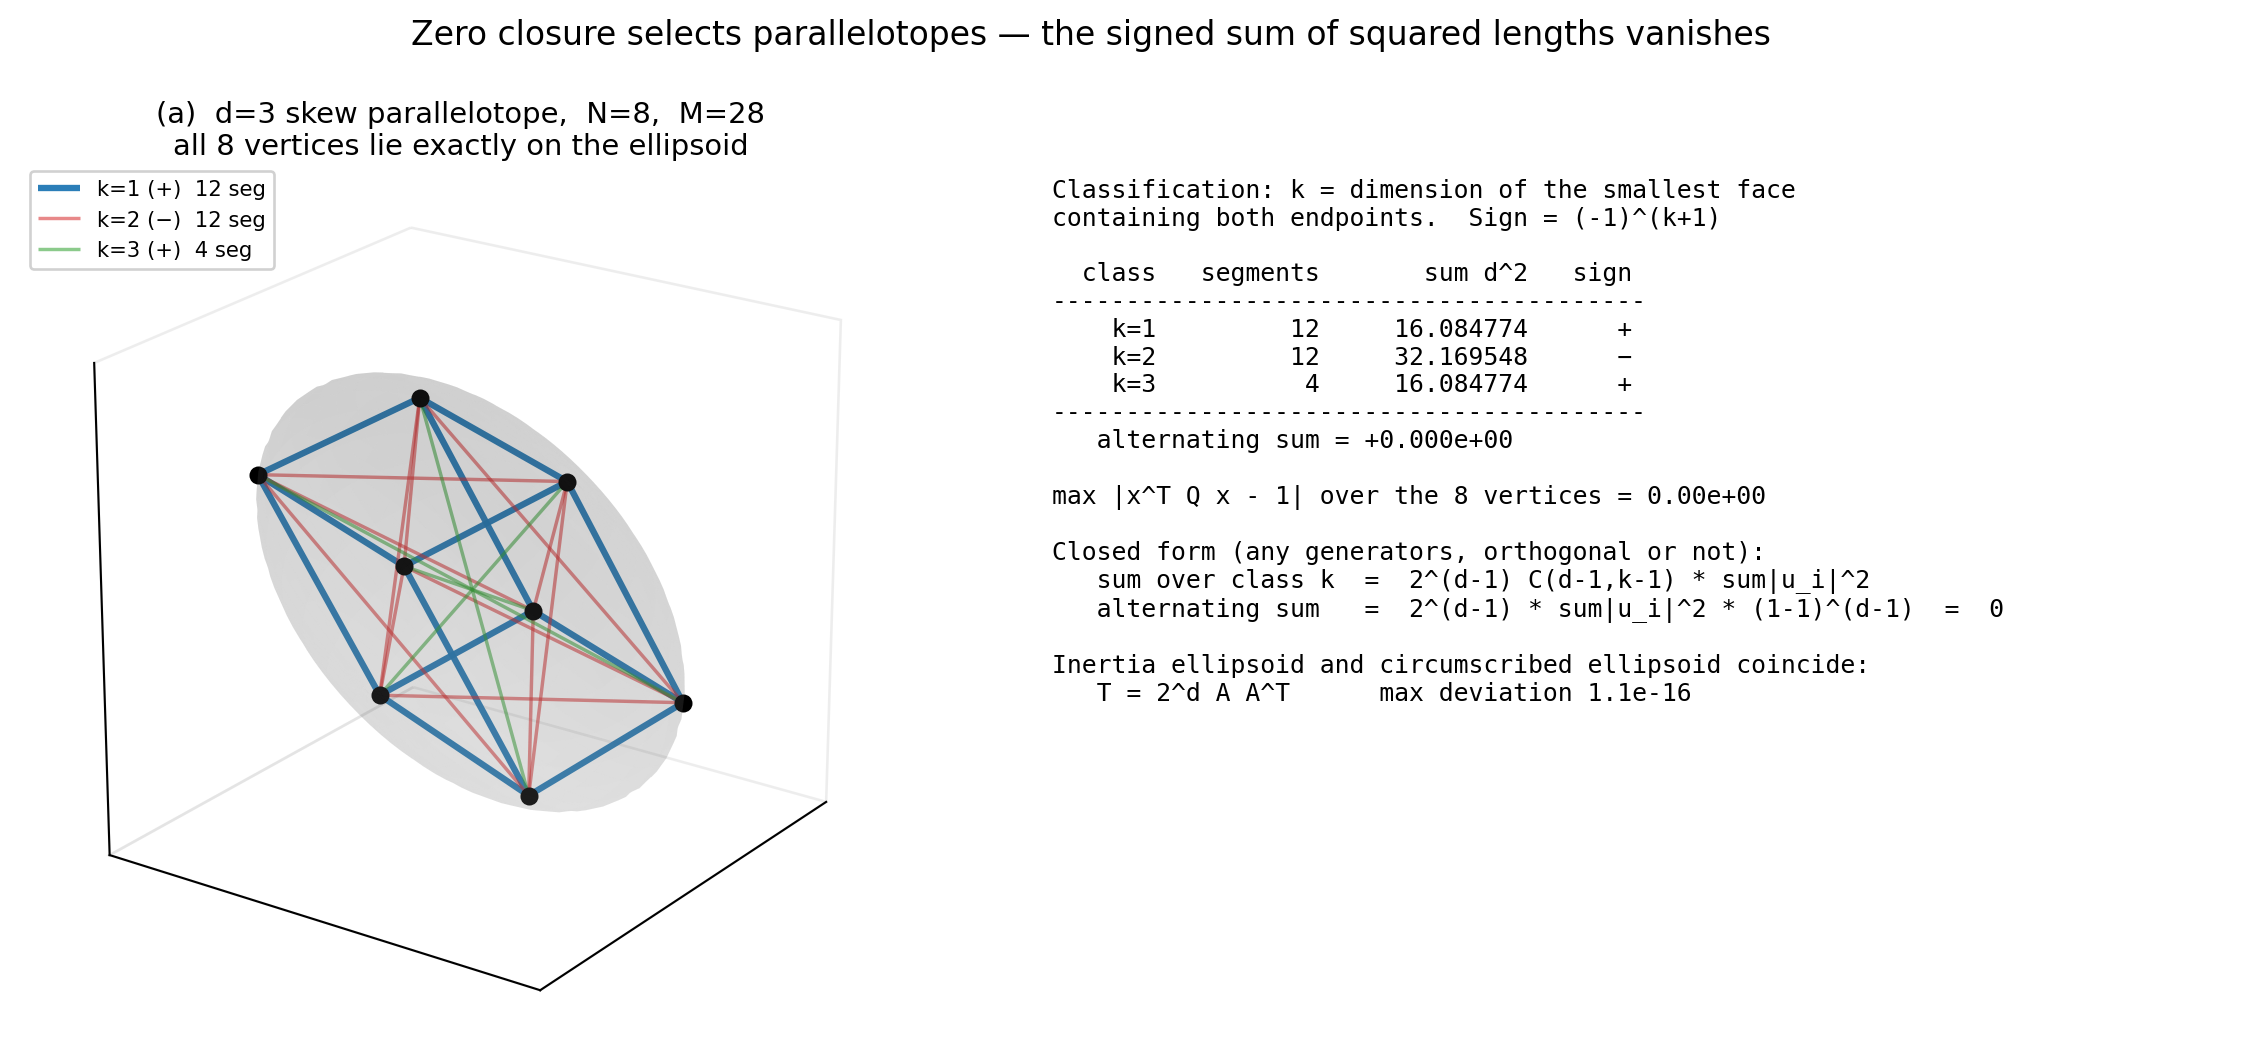
\includegraphics[keepaspectratio,alt={Figure 1}]{figures_v1/fig1_parallelotope_d3.png}}
\caption{Figure 1}
\end{figure}

A skew parallelepiped (\(d=3\), \(N=2^3=8\), \(M=28\)). The \(28\)
segments are coloured by the dimension \(k\) of the smallest face
containing both endpoints: \(k=1\) (edges) 12, \(k=2\) (face diagonals)
12, \(k=3\) (space diagonals) 4. The alternating sum with sign
\((-1)^{k+1}\) vanishes exactly.

\textbf{They must not be classified by length.} A skew parallelepiped
has 13 distinct values of length\(^2\), whereas the face-dimension
classification gives exactly 3 classes. The two coincide only for highly
symmetric figures such as the cube.

\paragraph{Figure 2 --- A four-dimensional parallelotope (projected to
three
dimensions)}\label{figure-2-a-four-dimensional-parallelotope-projected-to-three-dimensions}

\begin{figure}
\centering
\pandocbounded{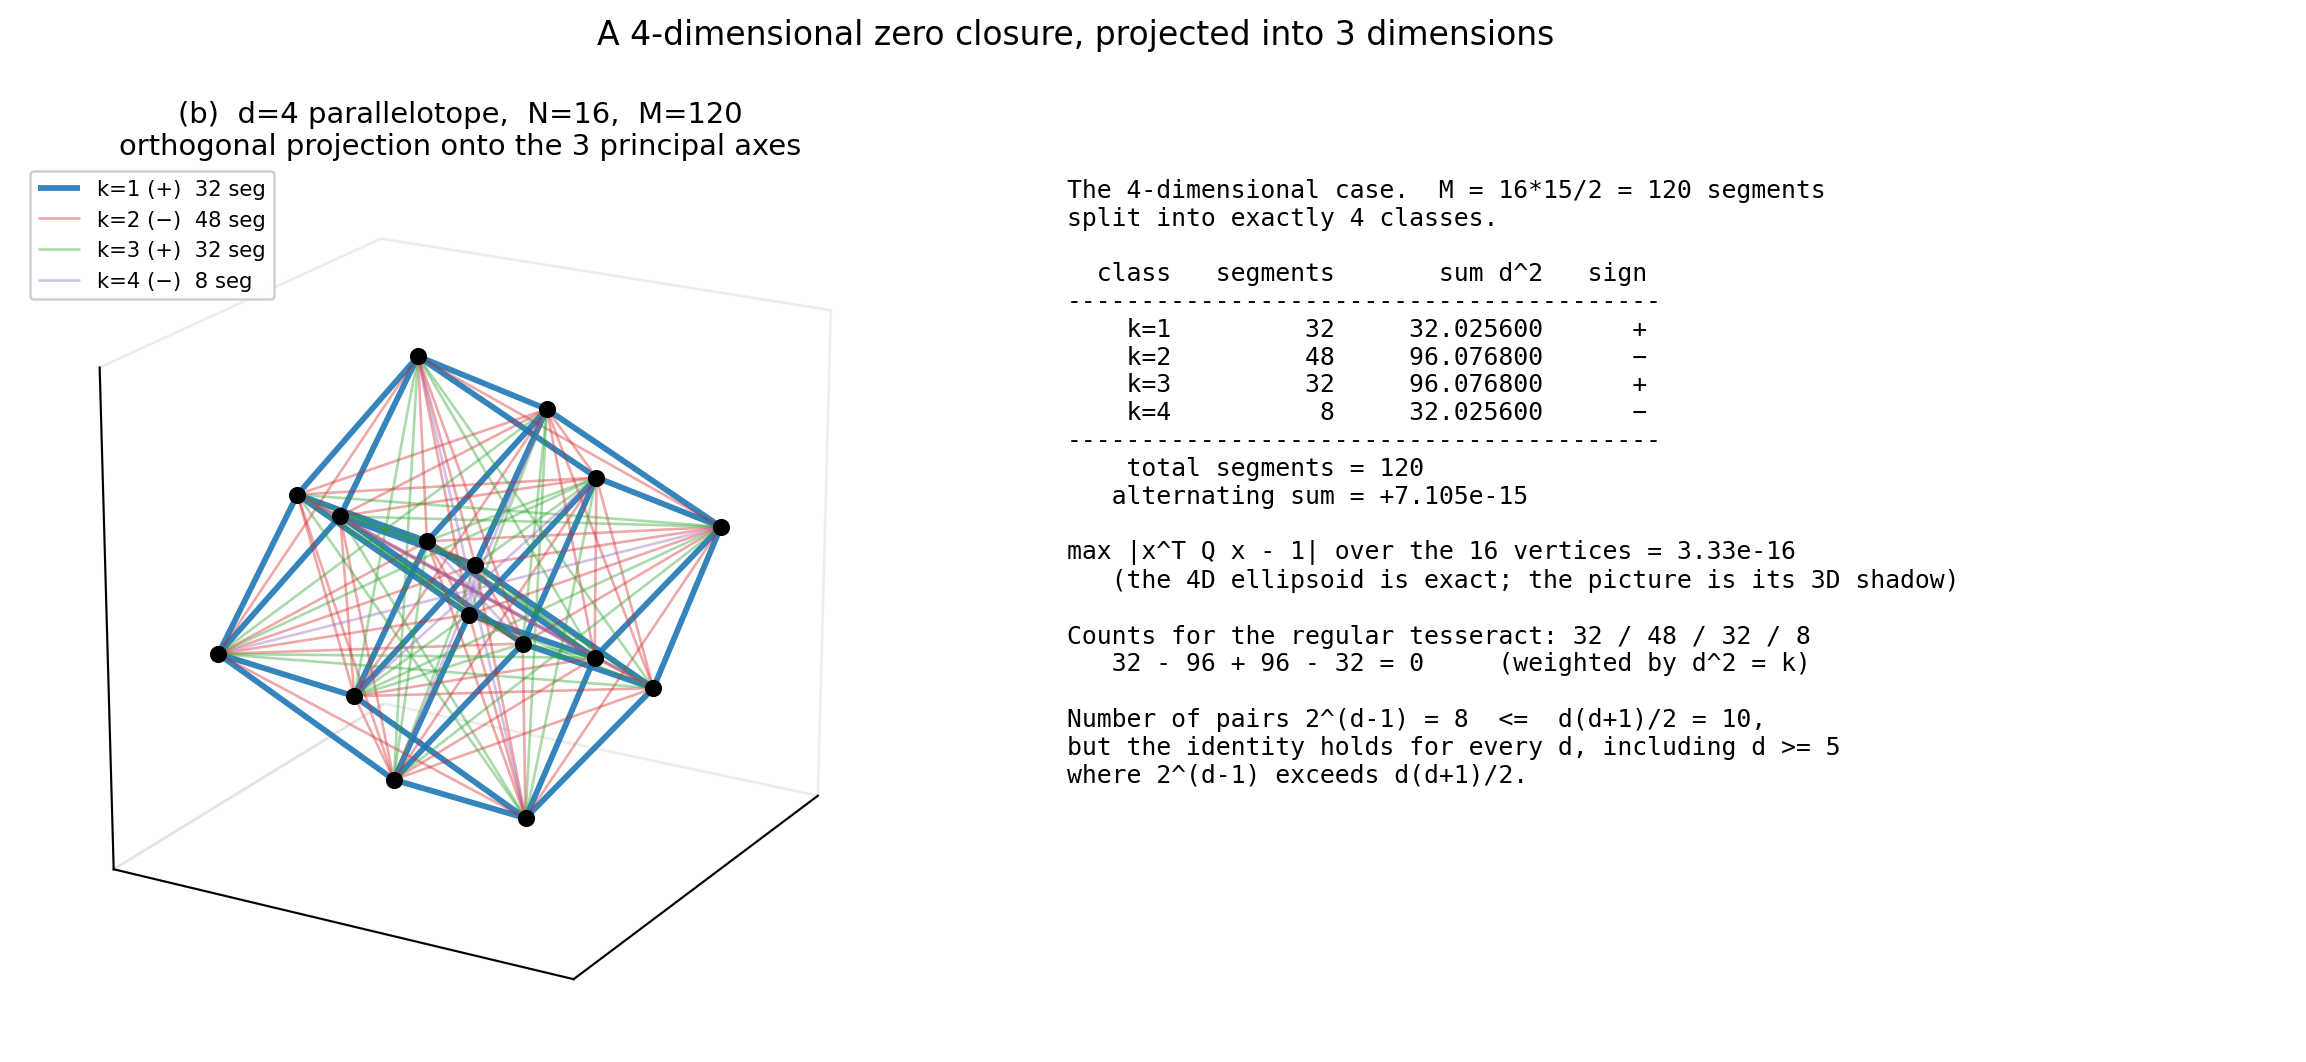
\includegraphics[keepaspectratio,alt={Figure 2}]{figures_v1/fig2_parallelotope_d4_projection.png}}
\caption{Figure 2}
\end{figure}

\(d=4\), \(N=16\), \(M=120\). The \(120\) segments split into 4 classes
(\(32/48/32/8\)). The \(\sum d^2\) are \(32.03/96.08/96.08/32.03\) and
the alternating sum is \(+7.1\times10^{-15}\).

\textbf{The picture is a shadow in three dimensions. The ellipsoid is
exact in four dimensions:
\(|x^{\mathsf T}Qx - 1| \le 3.3\times10^{-16}\) at all \(16\) vertices.}
Any apparent departure from an ellipse in the shadow is an effect of the
projection.

The number of pairs is \(2^{d-1} = 8 \le d(d+1)/2 = 10\) here, but the
identity also holds for \(d\ge5\) where \(2^{d-1}\) exceeds \(d(d+1)/2\)
(Claim 6B).

\paragraph{Figure 3 --- Counterexamples: lying on an ellipsoid is not
enough}\label{figure-3-counterexamples-lying-on-an-ellipsoid-is-not-enough}

\begin{figure}
\centering
\pandocbounded{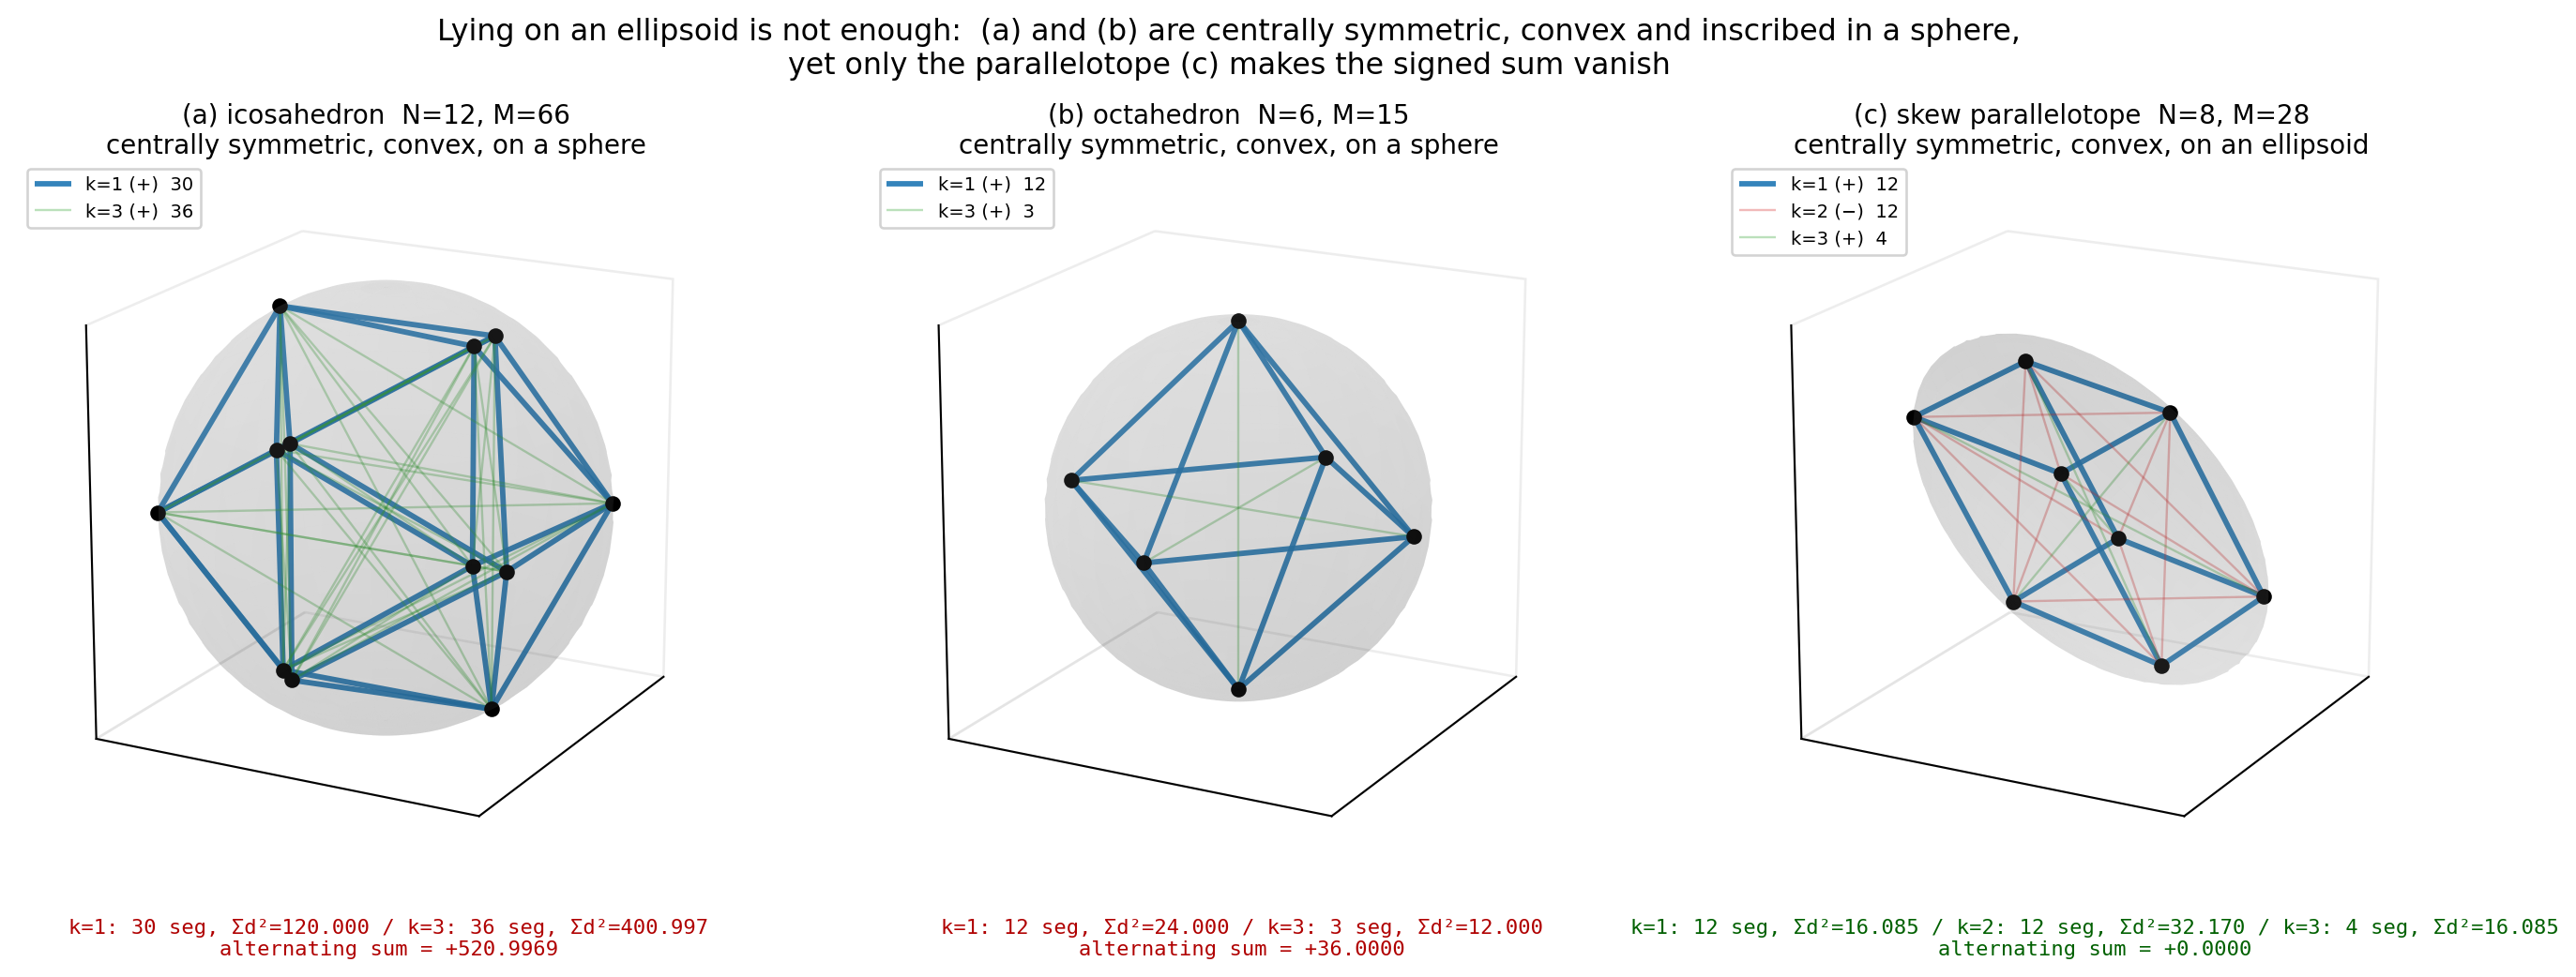
\includegraphics[keepaspectratio,alt={Figure 3}]{figures_v1/fig3_counterexamples.png}}
\caption{Figure 3}
\end{figure}

\begin{enumerate}
\def\labelenumi{(\alph{enumi})}
\tightlist
\item
  icosahedron (\(N=12\)), (b) octahedron (\(N=6\)), (c) skew
  parallelepiped (\(N=8\)). (a) and (b) are \textbf{centrally symmetric,
  convex, and lie on a sphere}, yet their alternating sums are
  \(+520.997\) and \(+36.000\), not zero. Only the parallelotope (c)
  gives zero (\(+0.0000\)).
\end{enumerate}

\textbf{What this figure shows is the single point that ``lying on an
ellipsoid'' and ``zero closure'' are different conditions.} Zero closure
is strictly stronger.

\paragraph{Figure 4 --- The zero-closure ellipsoid and what closure
fixes}\label{figure-4-the-zero-closure-ellipsoid-and-what-closure-fixes}

\begin{figure}
\centering
\pandocbounded{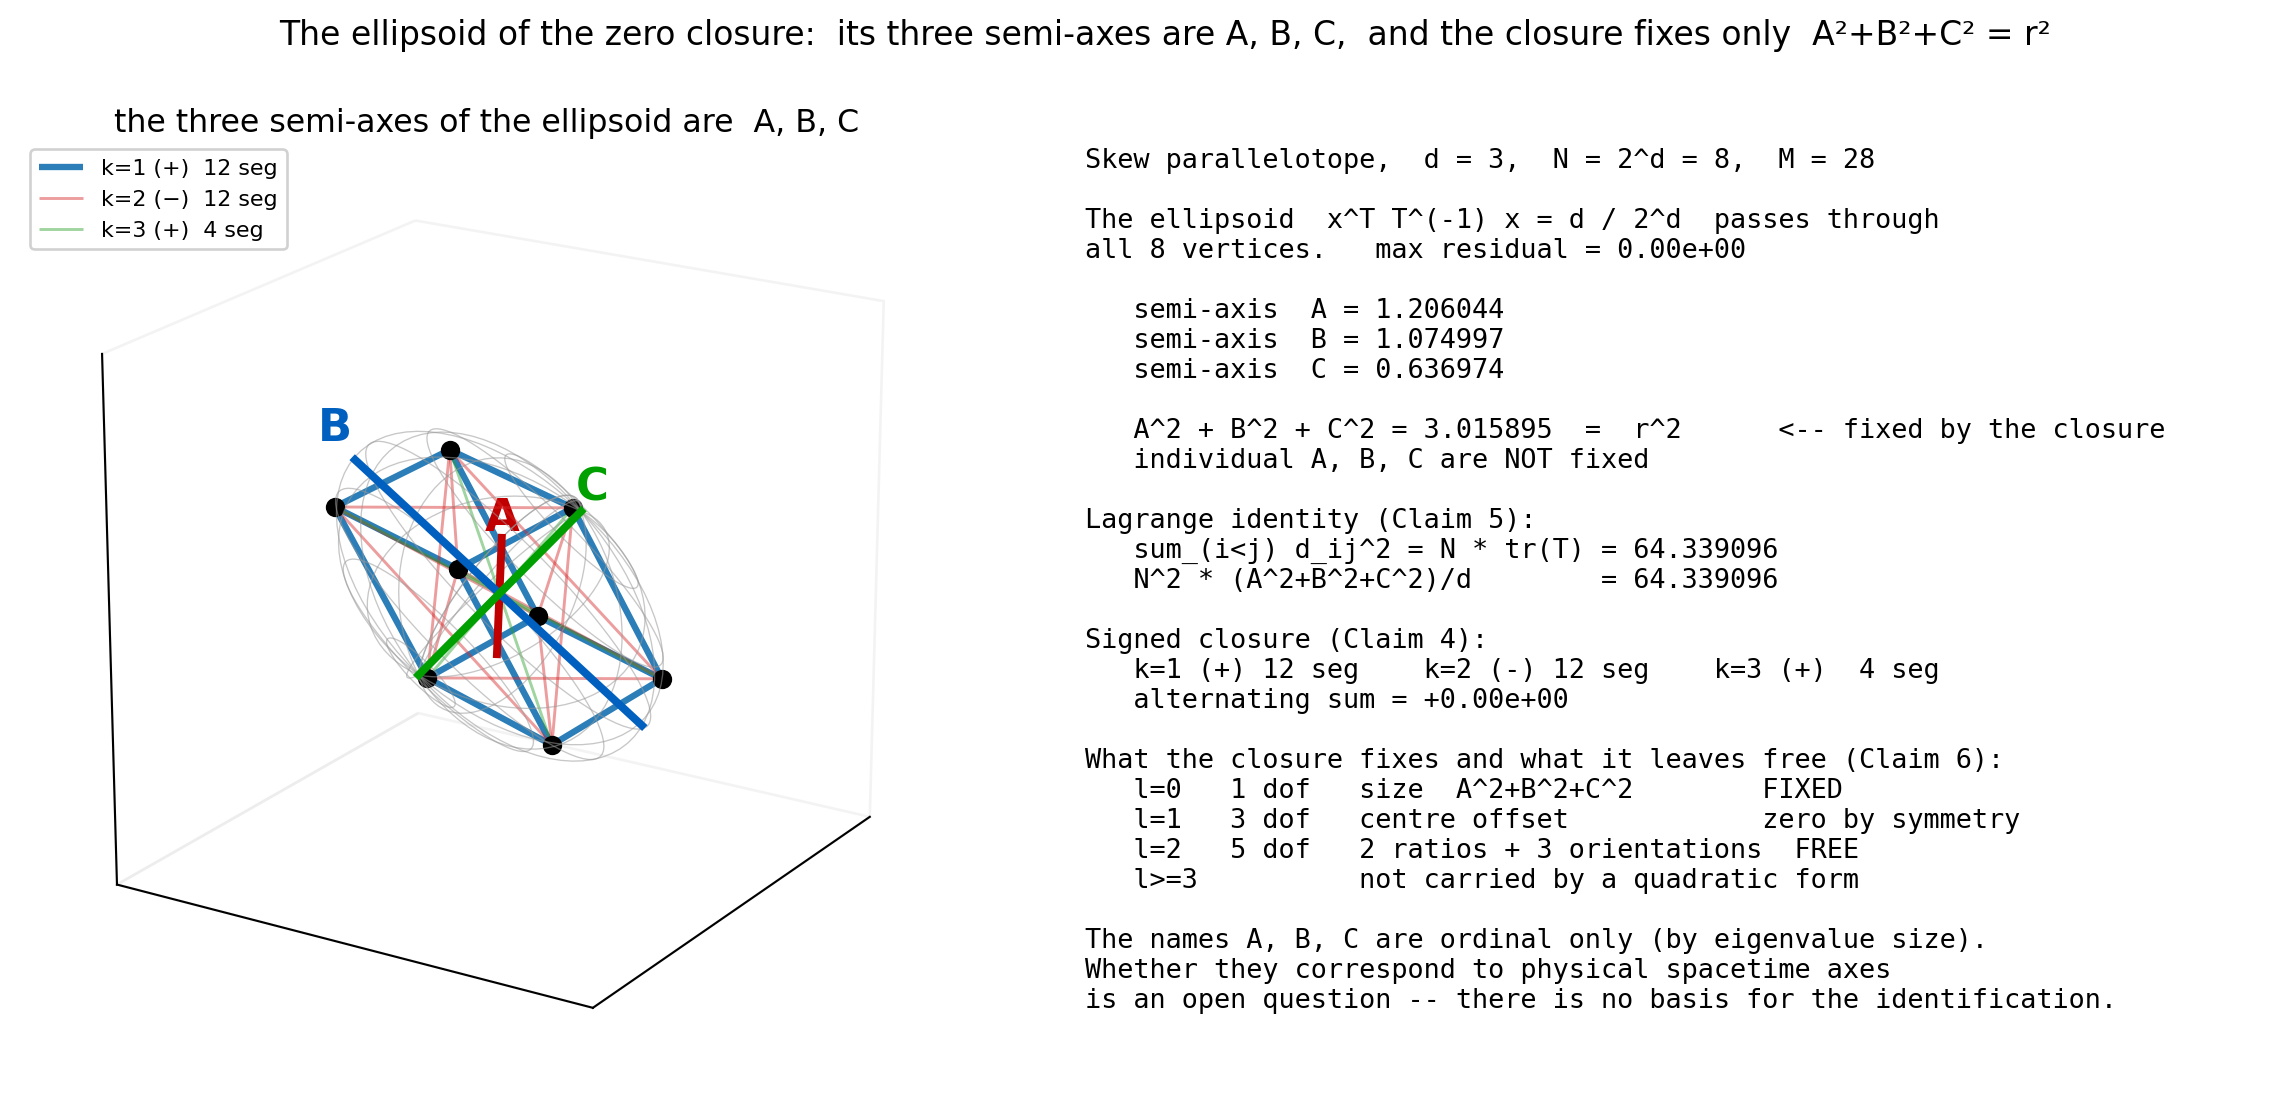
\includegraphics[keepaspectratio,alt={Figure 4}]{figures_v1/fig4_semiaxes_ABC.png}}
\caption{Figure 4}
\end{figure}

The circumscribed ellipsoid of a parallelotope coincides with the
\textbf{normalised inertia ellipsoid (\(c=d/N\))} (Claim 6B, §0
definitions). Write the semi-axes as \(A,B,C\). \textbf{Zero closure
\(S(D)=0\) imposes one condition on the signed distance sum but does not
fix the value of \(A^2+B^2+C^2\).} Adding the fixing of \(C\) or a
normalisation fixes the unsigned total square \(U(D)=2C\), and
correspondingly the trace of the inertia tensor, i.e.~\(l=0\) (Claim 5).
The individual \(A,B,C\) are not determined. In multipoles, one \(l=0\)
degree of freedom is fixed (by fixing \(C\) or normalisation) and the
five \(l=2\) degrees (2 shape + 3 orientation) remain free (Claim 6).
\textbf{The decomposition of \(T\) has only the two pieces
\(l=0\oplus l=2\); \(l=1\) (the first moment) is not a component of
\(T\) and is zero by definition in centroid coordinates} (the correction
in Claim 6).

The names \(A,B,C\) are ordinals by eigenvalue magnitude. Correspondence
with physical spacetime is an open task (§0B, Claim 12).

\subsubsection{5.2 Numerical model figures (run
results)}\label{numerical-model-figures-run-results}

Conditions: mode = electron, \(N=16=2^4\), \(\delta=0.1\), \(T=40000\).
Matter side (\texttt{\_m\_}) and vacuum control (\texttt{\_v\_}). Each
figure has four panels.

{\def\LTcaptype{none} % do not increment counter
\begin{longtable}[]{@{}
  >{\raggedright\arraybackslash}p{(\linewidth - 2\tabcolsep) * \real{0.5000}}
  >{\raggedright\arraybackslash}p{(\linewidth - 2\tabcolsep) * \real{0.5000}}@{}}
\toprule\noalign{}
\begin{minipage}[b]{\linewidth}\raggedright
Panel
\end{minipage} & \begin{minipage}[b]{\linewidth}\raggedright
Content
\end{minipage} \\
\midrule\noalign{}
\endhead
\bottomrule\noalign{}
\endlastfoot
(a) & absolute scale; frame fixed at \(\pm0.17\). The same frame at
every \(\tau\), so change of size relative to the frame is change of
scale \\
(b) & normalised by \(r_{\rm rms}\); frame fixed at \(\pm1.1\). Compares
shape only \\
(c) & scale history (logarithmic); the current \(\tau\) marked by a
vertical line \\
(d) & history of all 15 principal axes; above \(0\) real, below \(0\)
imaginary \\
\end{longtable}
}

\begin{quote}
\textbf{On the frame values (correcting an error of v3)}: the
\texttt{half-range} in the figure title is the value of the launch
argument \texttt{-\/-absmax}; the actual frame is that divided by
\texttt{-\/-zoom} (default 2.0). v3 wrote \(\pm0.28\)/\(\pm2.2\), but
the actual frames were \(\pm0.14\)/\(\pm1.1\). The v4 \(N=16\) figures
use \texttt{-\/-absmax\ 0.34\ -\/-zoom\ 2} (actual frame \(\pm0.17\)) so
that all vertices fit inside.
\end{quote}

Vertex colour shows the deviation \(s_i\) (blue inside the ellipsoid,
red outside, white on it); segment colour shows the relation length
\(|z|\).

\paragraph{Figures 5--8 --- Four time points on the matter
side}\label{figures-58-four-time-points-on-the-matter-side}

{\def\LTcaptype{none} % do not increment counter
\begin{longtable}[]{@{}
  >{\raggedright\arraybackslash}p{(\linewidth - 2\tabcolsep) * \real{0.5000}}
  >{\raggedright\arraybackslash}p{(\linewidth - 2\tabcolsep) * \real{0.5000}}@{}}
\toprule\noalign{}
\begin{minipage}[b]{\linewidth}\raggedright
\(\tau\)
\end{minipage} & \begin{minipage}[b]{\linewidth}\raggedright
Figure
\end{minipage} \\
\midrule\noalign{}
\endhead
\bottomrule\noalign{}
\endlastfoot
0 (start) &
\pandocbounded{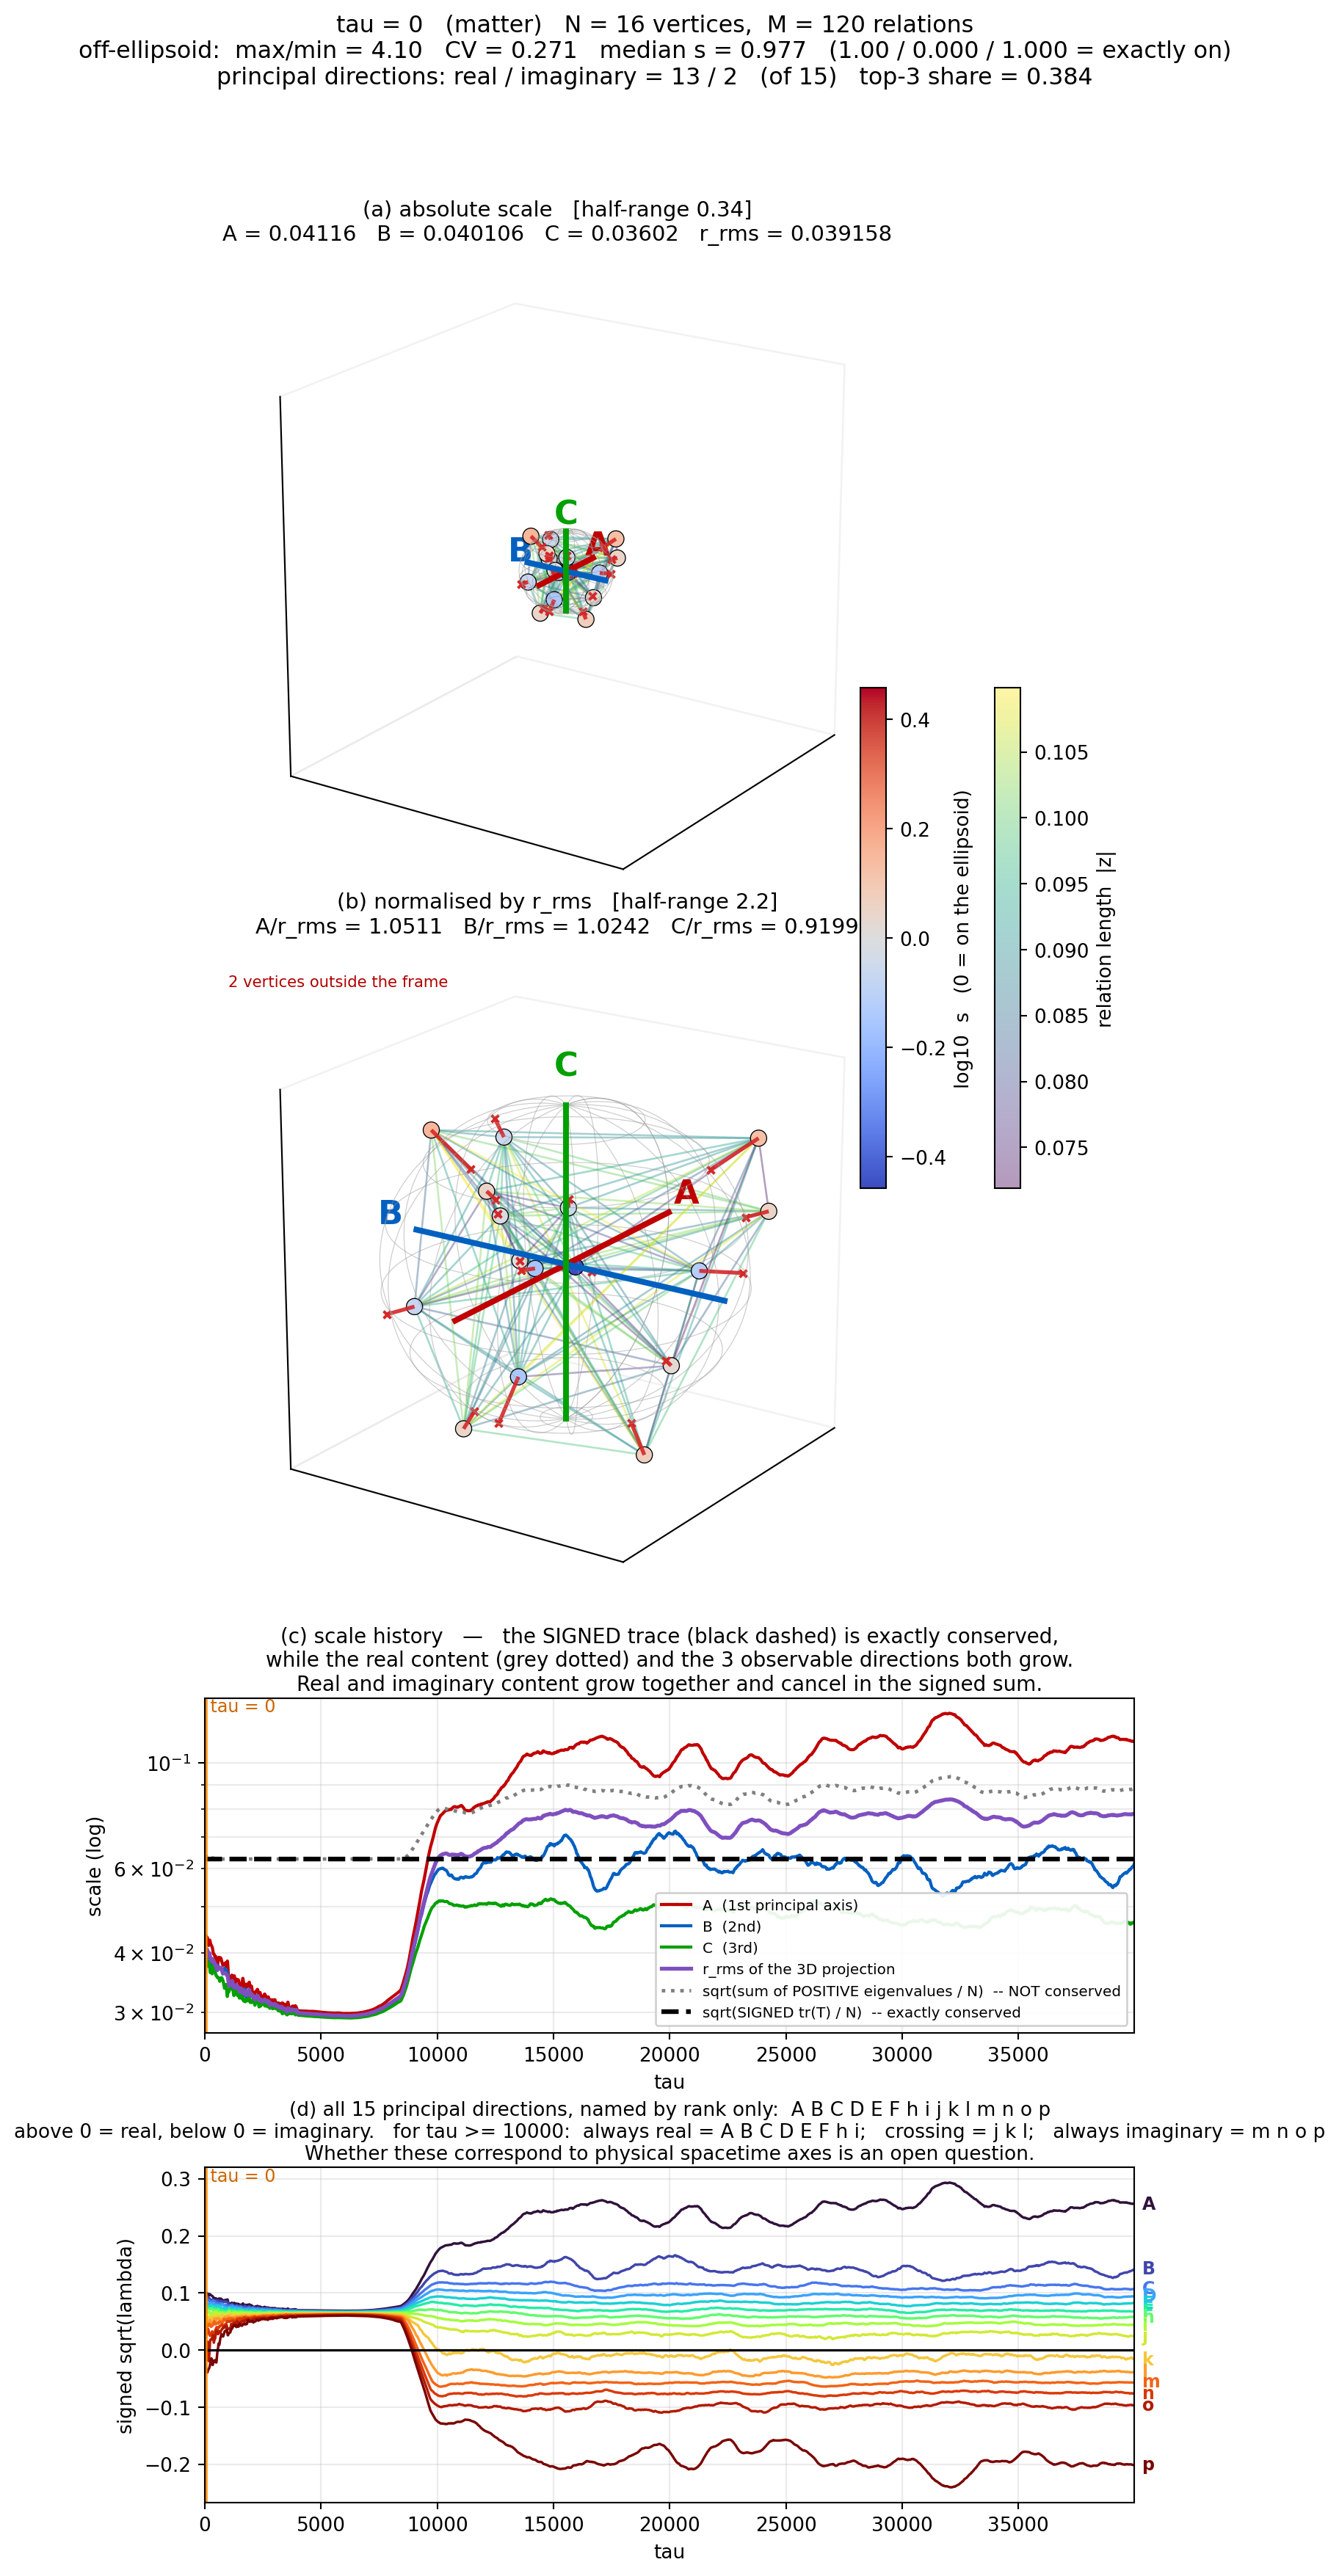
\includegraphics[keepaspectratio,alt={matter τ=0}]{複製_ダンプ版_v1/次元の生成構造/対照実験_N掃引1to20_三系_v2/figures_tau/fig_ellipsoid_tau00000_electron_T40000_d0.1_rep-dump40k16_N16_m_v1.png}} \\
4000 (pre-transition) &
\pandocbounded{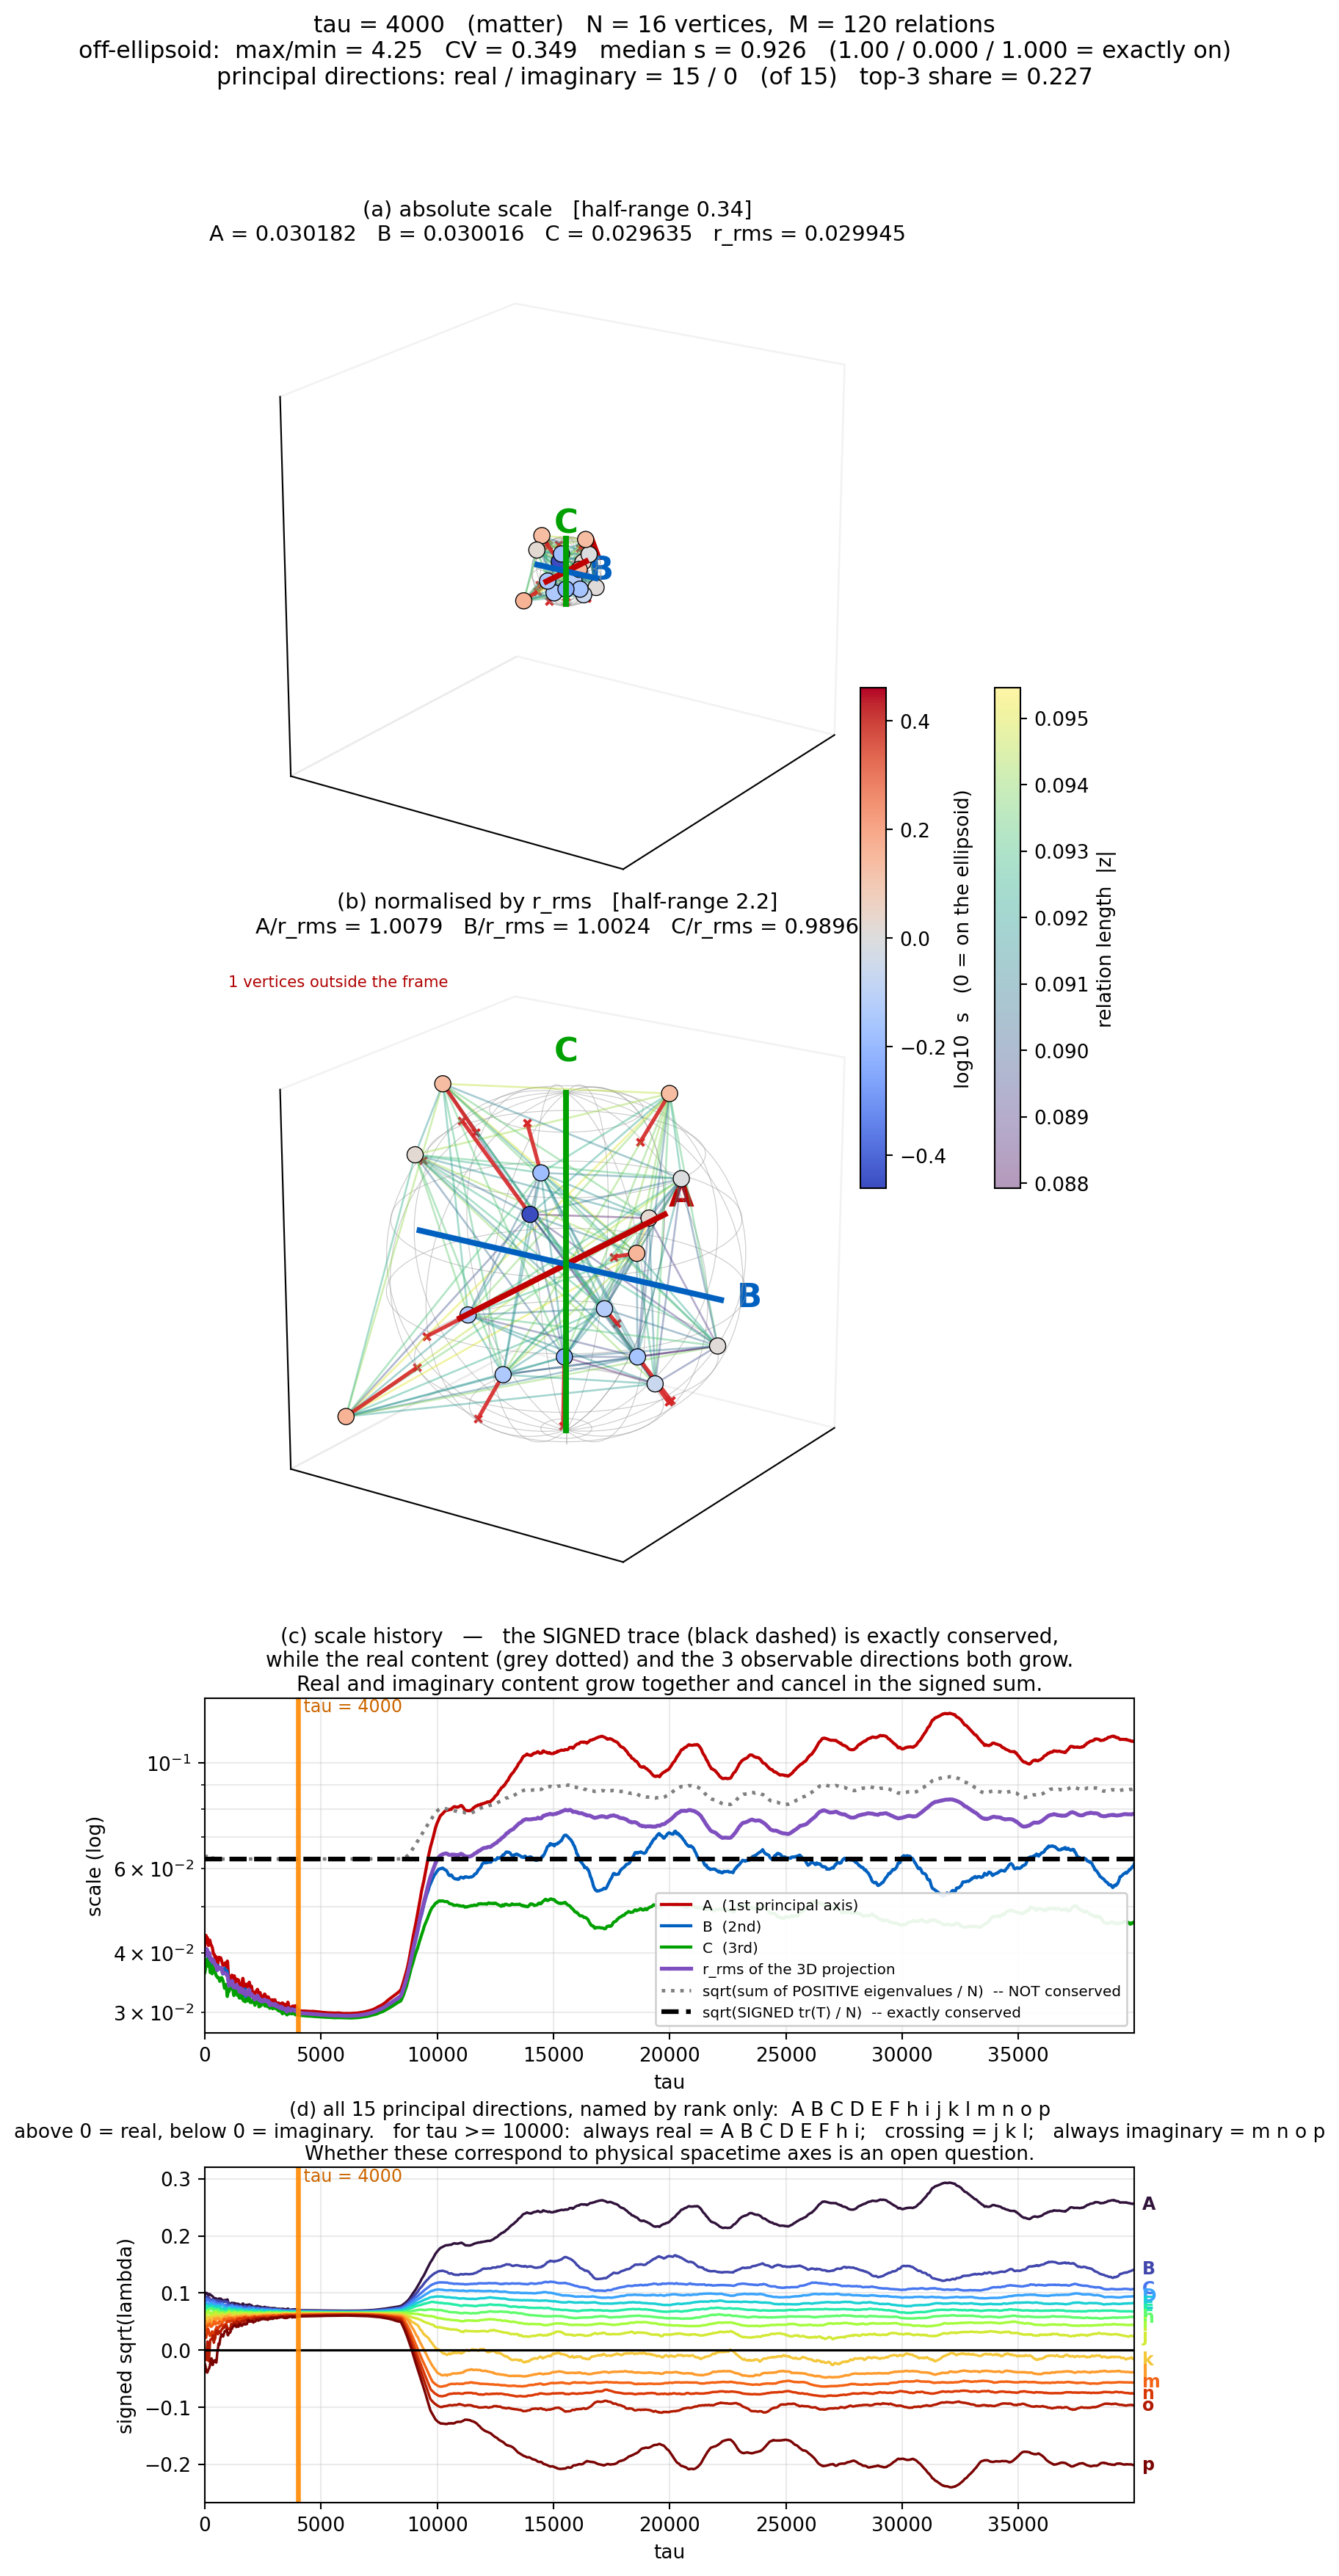
\includegraphics[keepaspectratio,alt={matter τ=4000}]{複製_ダンプ版_v1/次元の生成構造/対照実験_N掃引1to20_三系_v2/figures_tau/fig_ellipsoid_tau04000_electron_T40000_d0.1_rep-dump40k16_N16_m_v1.png}} \\
9487 (just after transition) &
\pandocbounded{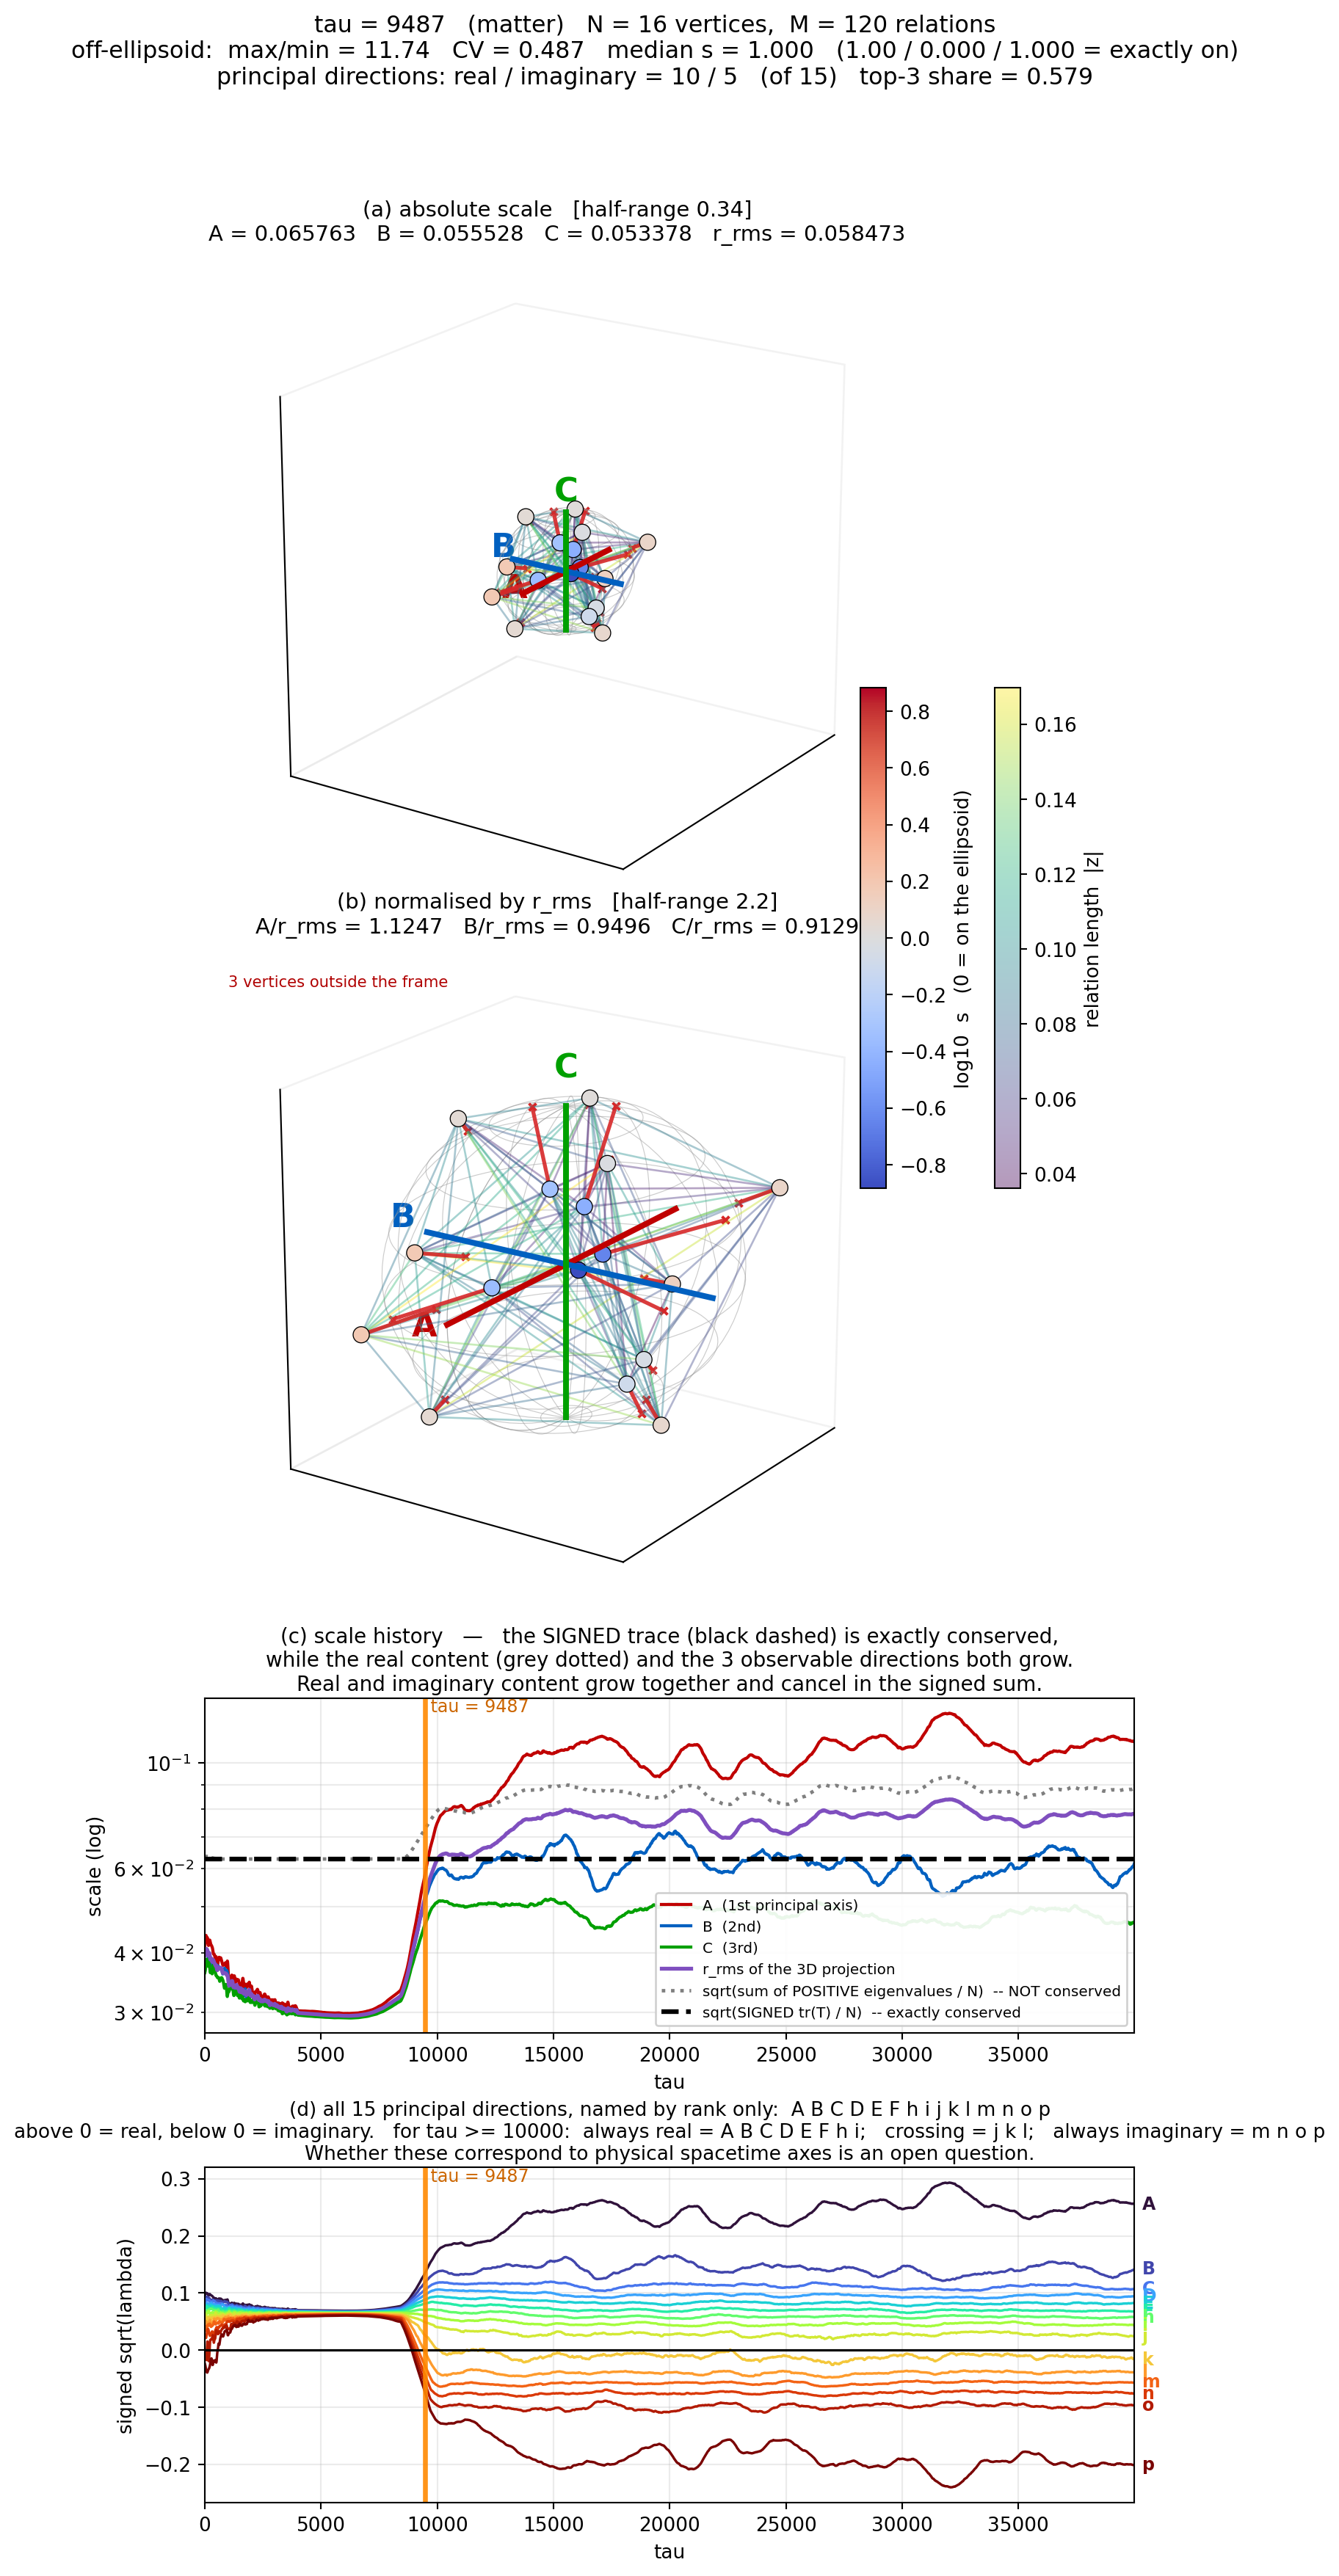
\includegraphics[keepaspectratio,alt={matter τ=9487}]{複製_ダンプ版_v1/次元の生成構造/対照実験_N掃引1to20_三系_v2/figures_tau/fig_ellipsoid_tau09487_electron_T40000_d0.1_rep-dump40k16_N16_m_v1.png}} \\
39991 (end) &
\pandocbounded{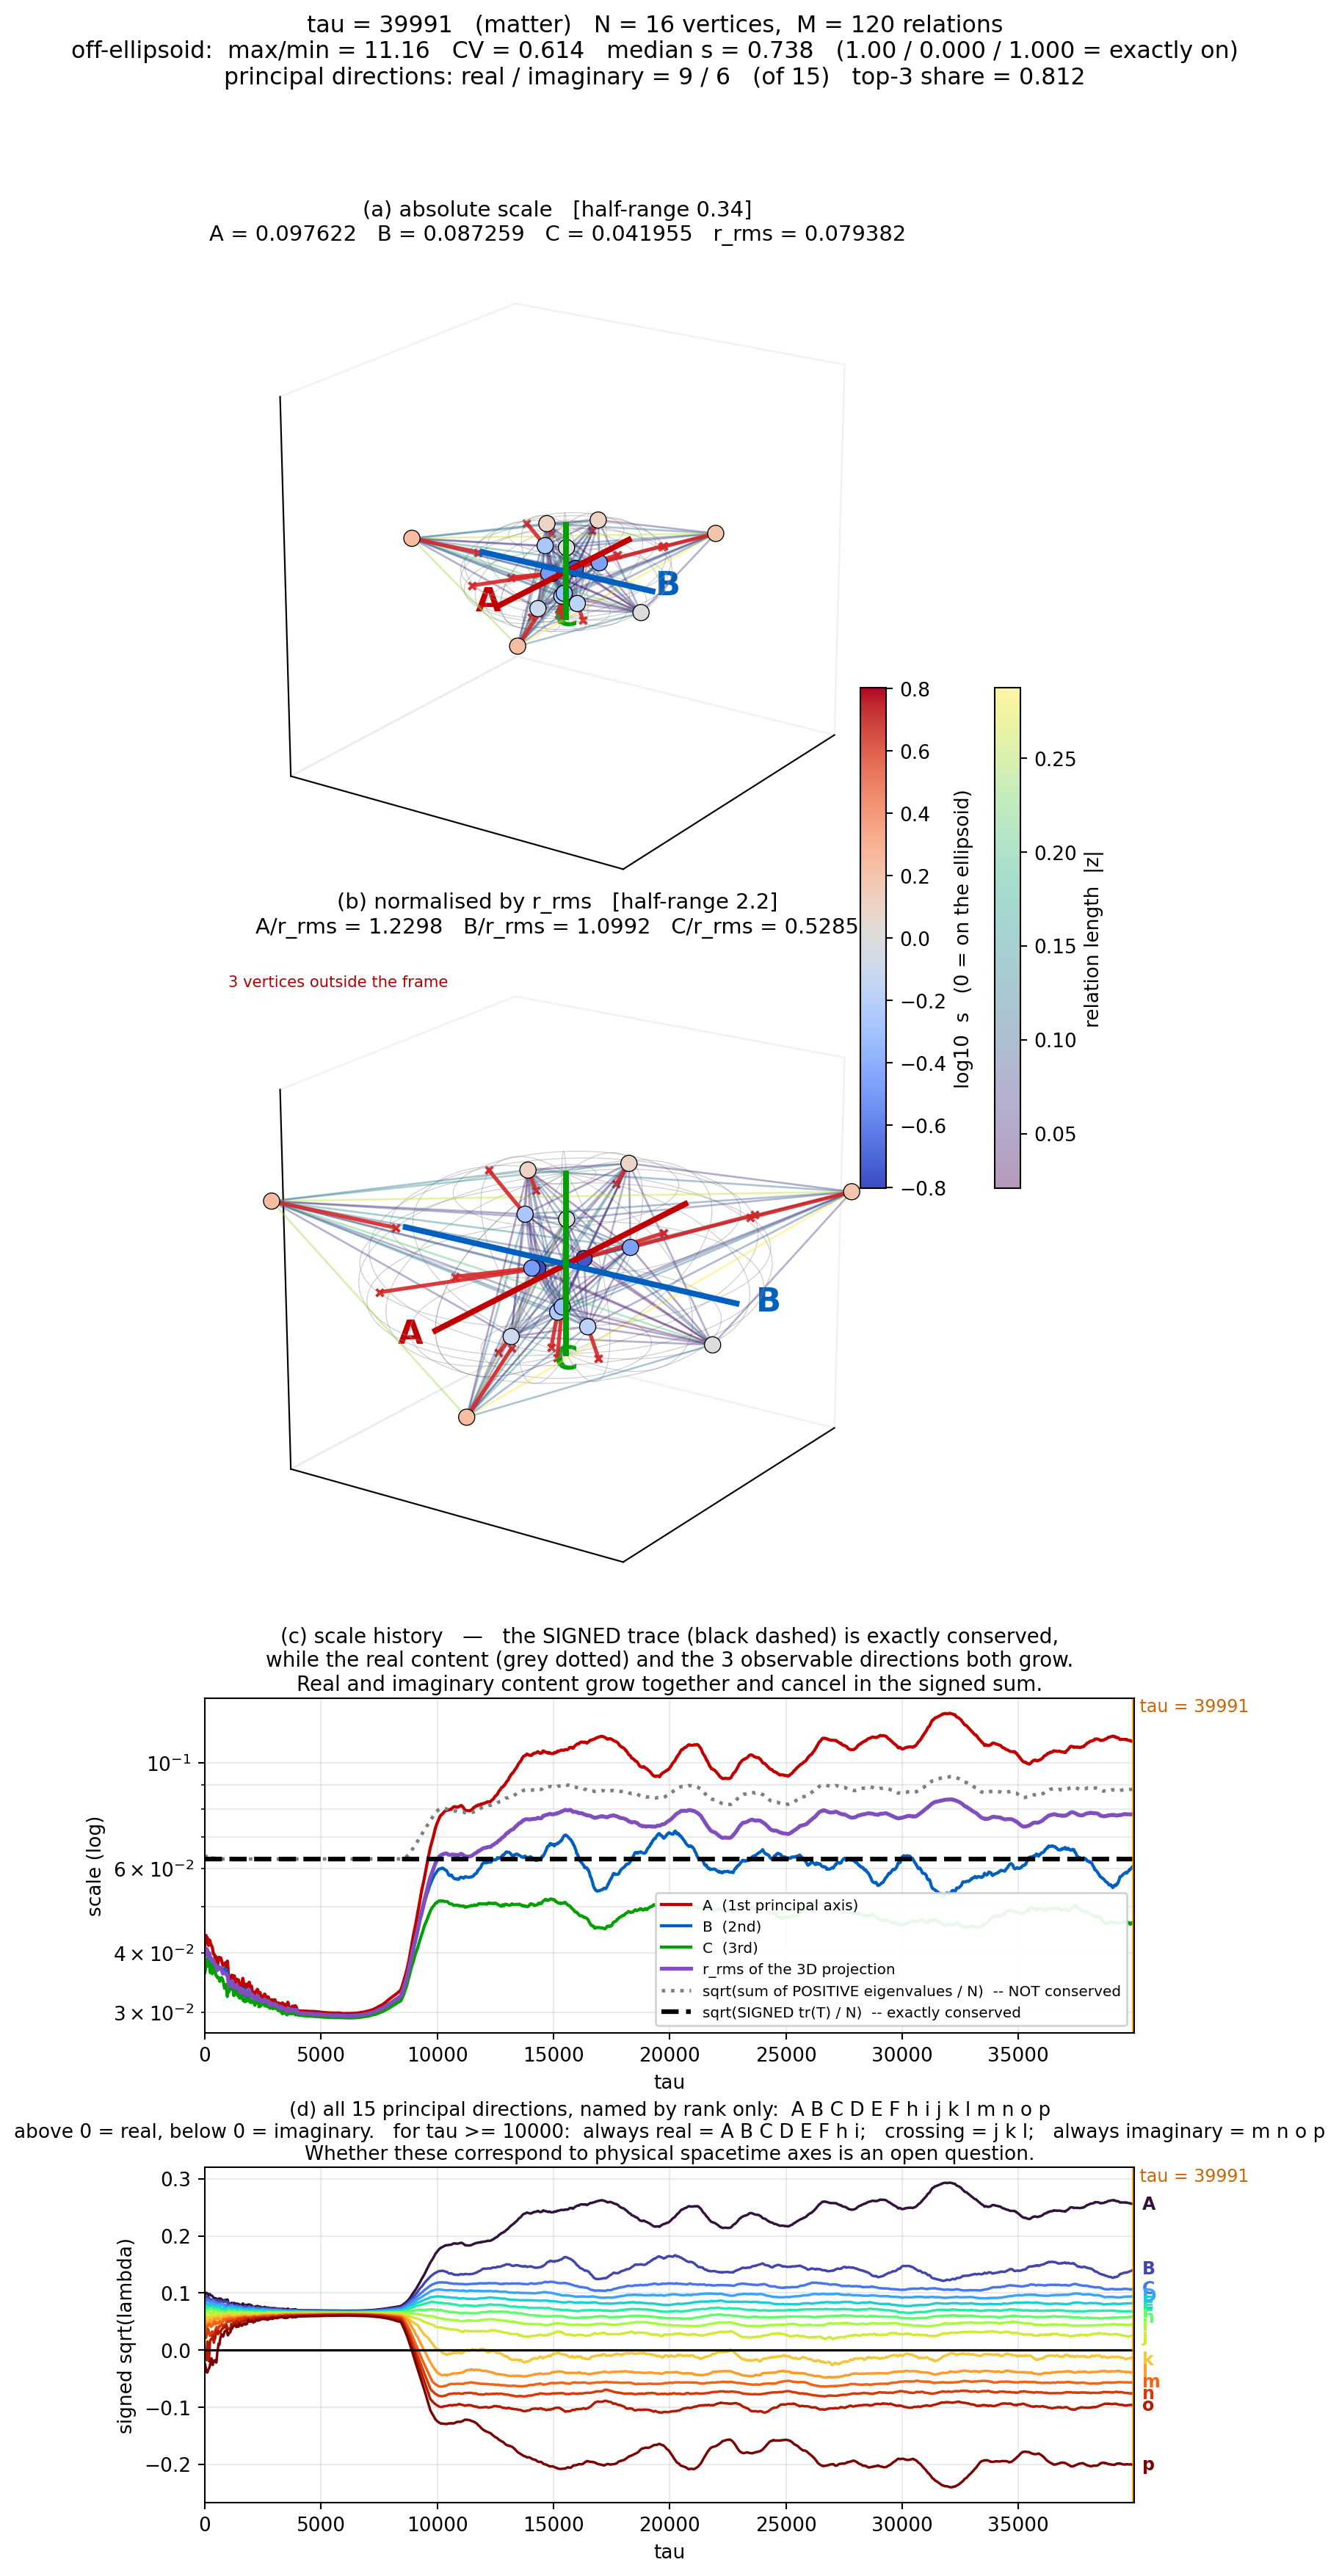
\includegraphics[keepaspectratio,alt={matter τ=39991}]{複製_ダンプ版_v1/次元の生成構造/対照実験_N掃引1to20_三系_v2/figures_tau/fig_ellipsoid_tau39991_electron_T40000_d0.1_rep-dump40k16_N16_m_v1.png}} \\
\end{longtable}
}

\paragraph{Figures 9--12 --- Four time points of the vacuum
control}\label{figures-912-four-time-points-of-the-vacuum-control}

{\def\LTcaptype{none} % do not increment counter
\begin{longtable}[]{@{}
  >{\raggedright\arraybackslash}p{(\linewidth - 2\tabcolsep) * \real{0.5000}}
  >{\raggedright\arraybackslash}p{(\linewidth - 2\tabcolsep) * \real{0.5000}}@{}}
\toprule\noalign{}
\begin{minipage}[b]{\linewidth}\raggedright
\(\tau\)
\end{minipage} & \begin{minipage}[b]{\linewidth}\raggedright
Figure
\end{minipage} \\
\midrule\noalign{}
\endhead
\bottomrule\noalign{}
\endlastfoot
0 &
\pandocbounded{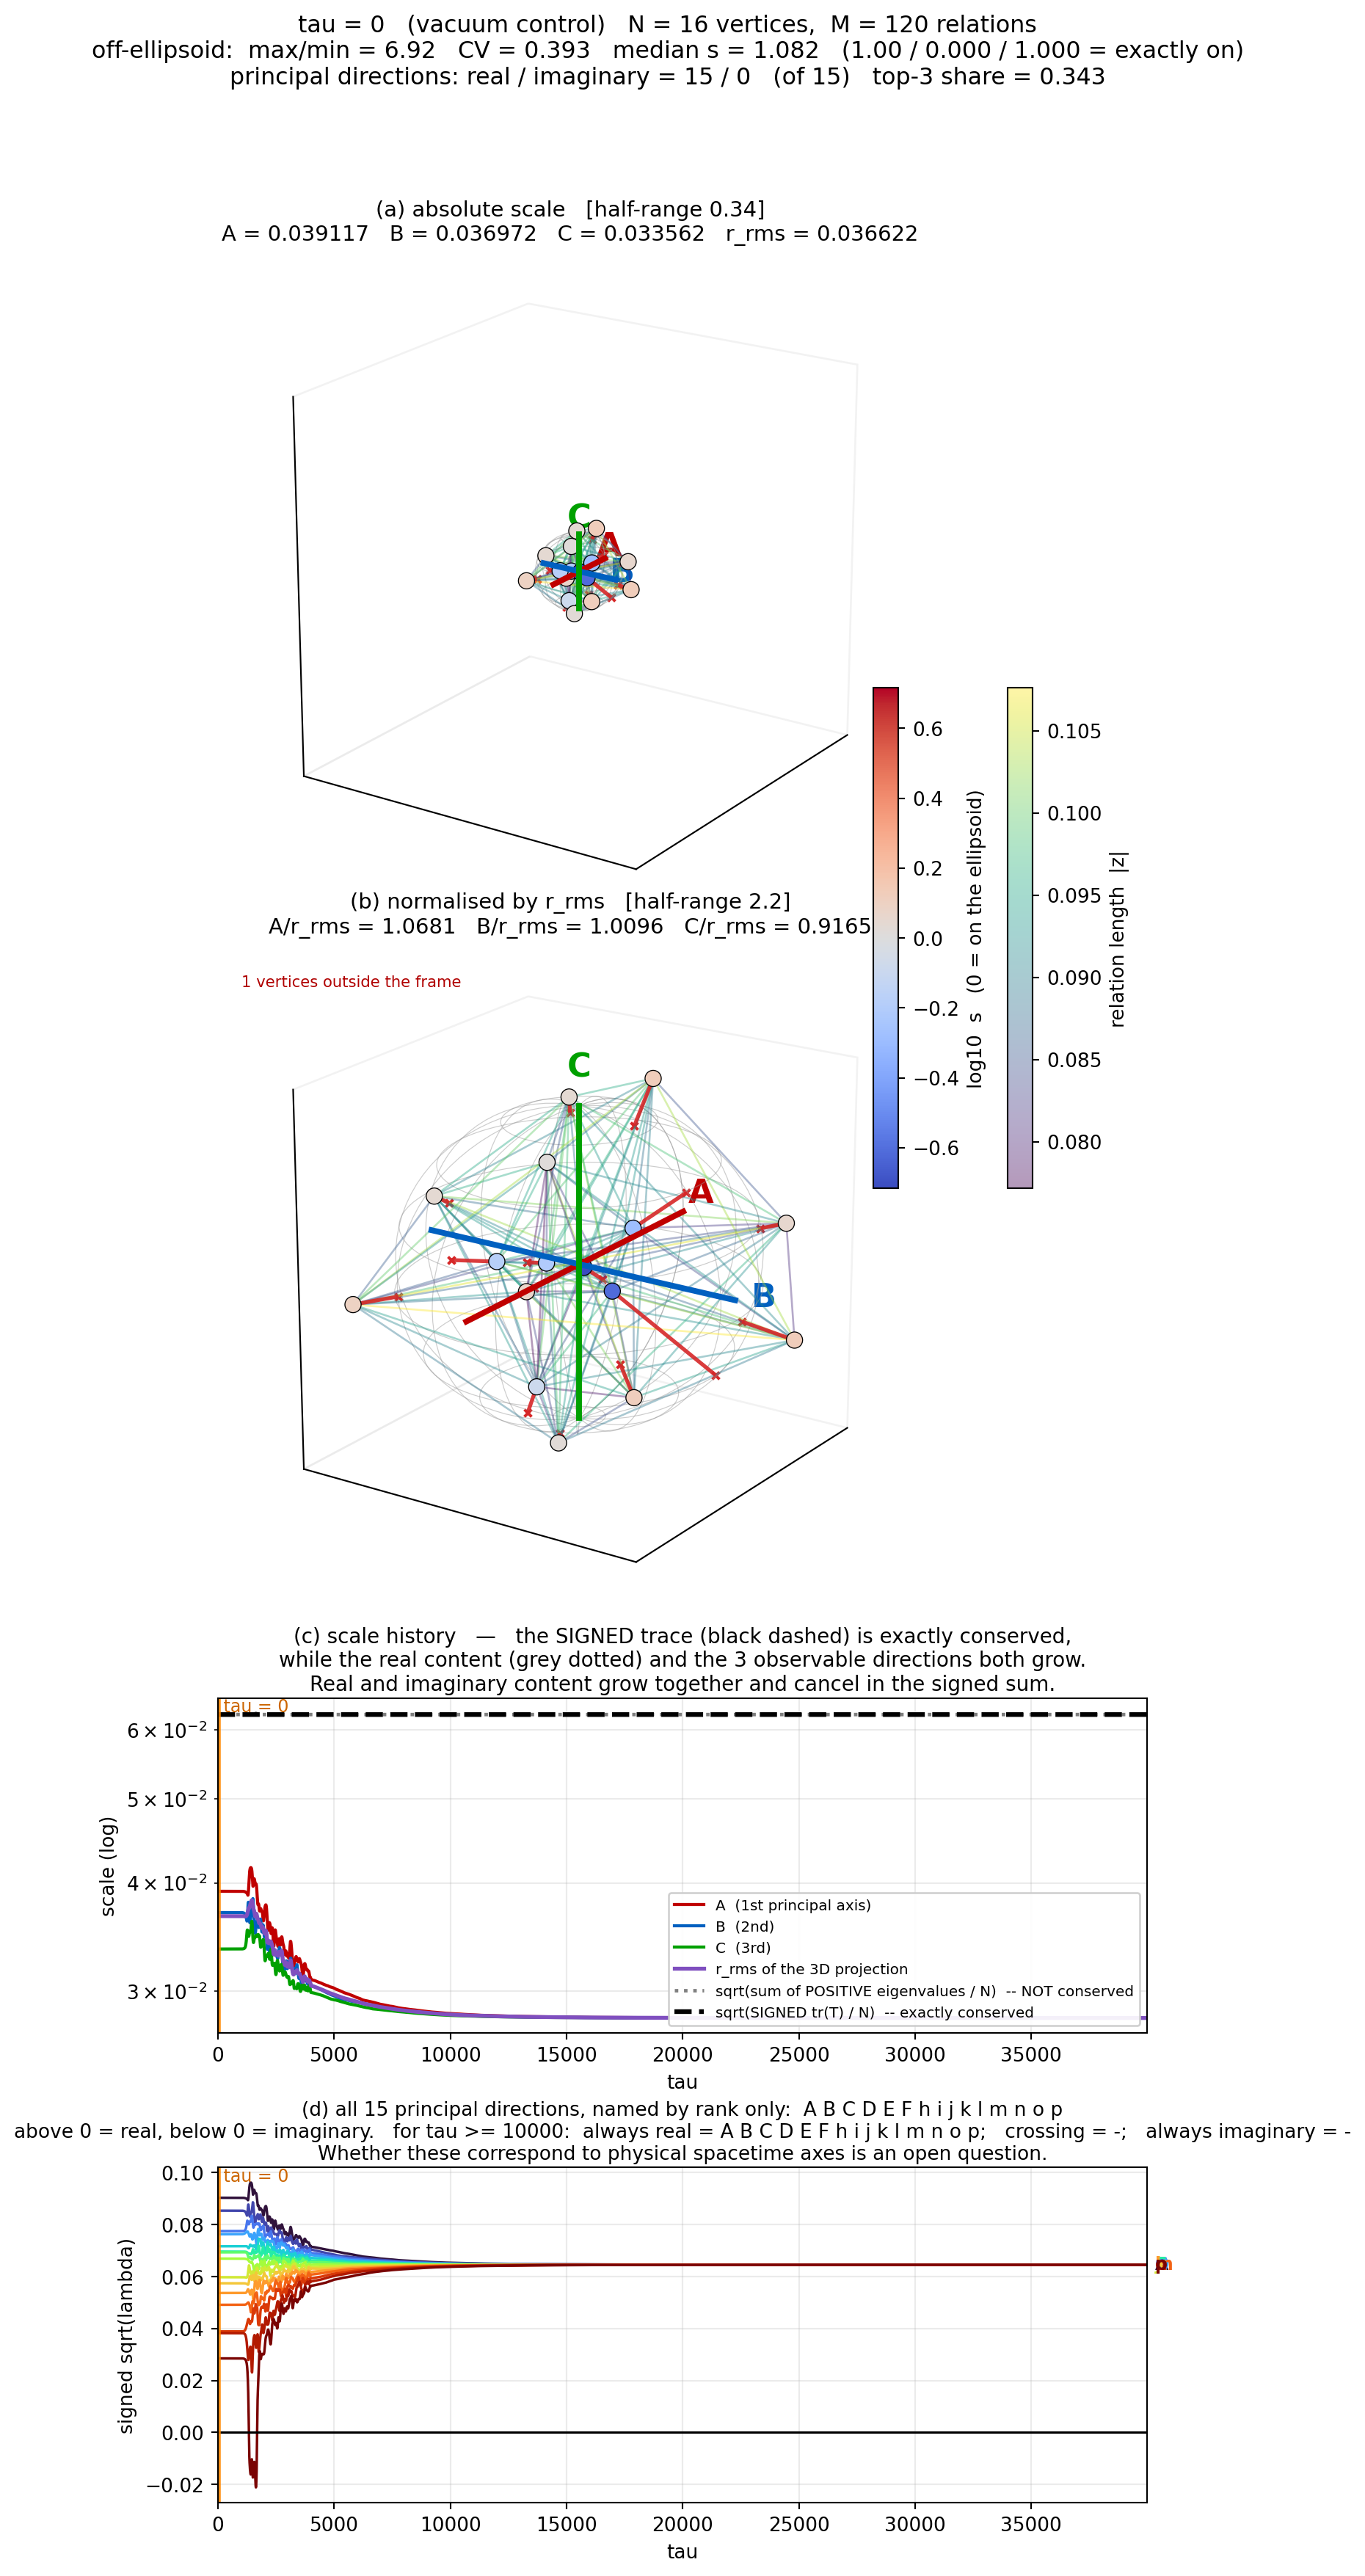
\includegraphics[keepaspectratio,alt={vacuum τ=0}]{複製_ダンプ版_v1/次元の生成構造/対照実験_N掃引1to20_三系_v2/figures_tau/fig_ellipsoid_tau00000_electron_T40000_d0.1_rep-dump40k16_N16_v_v1.png}} \\
4000 &
\pandocbounded{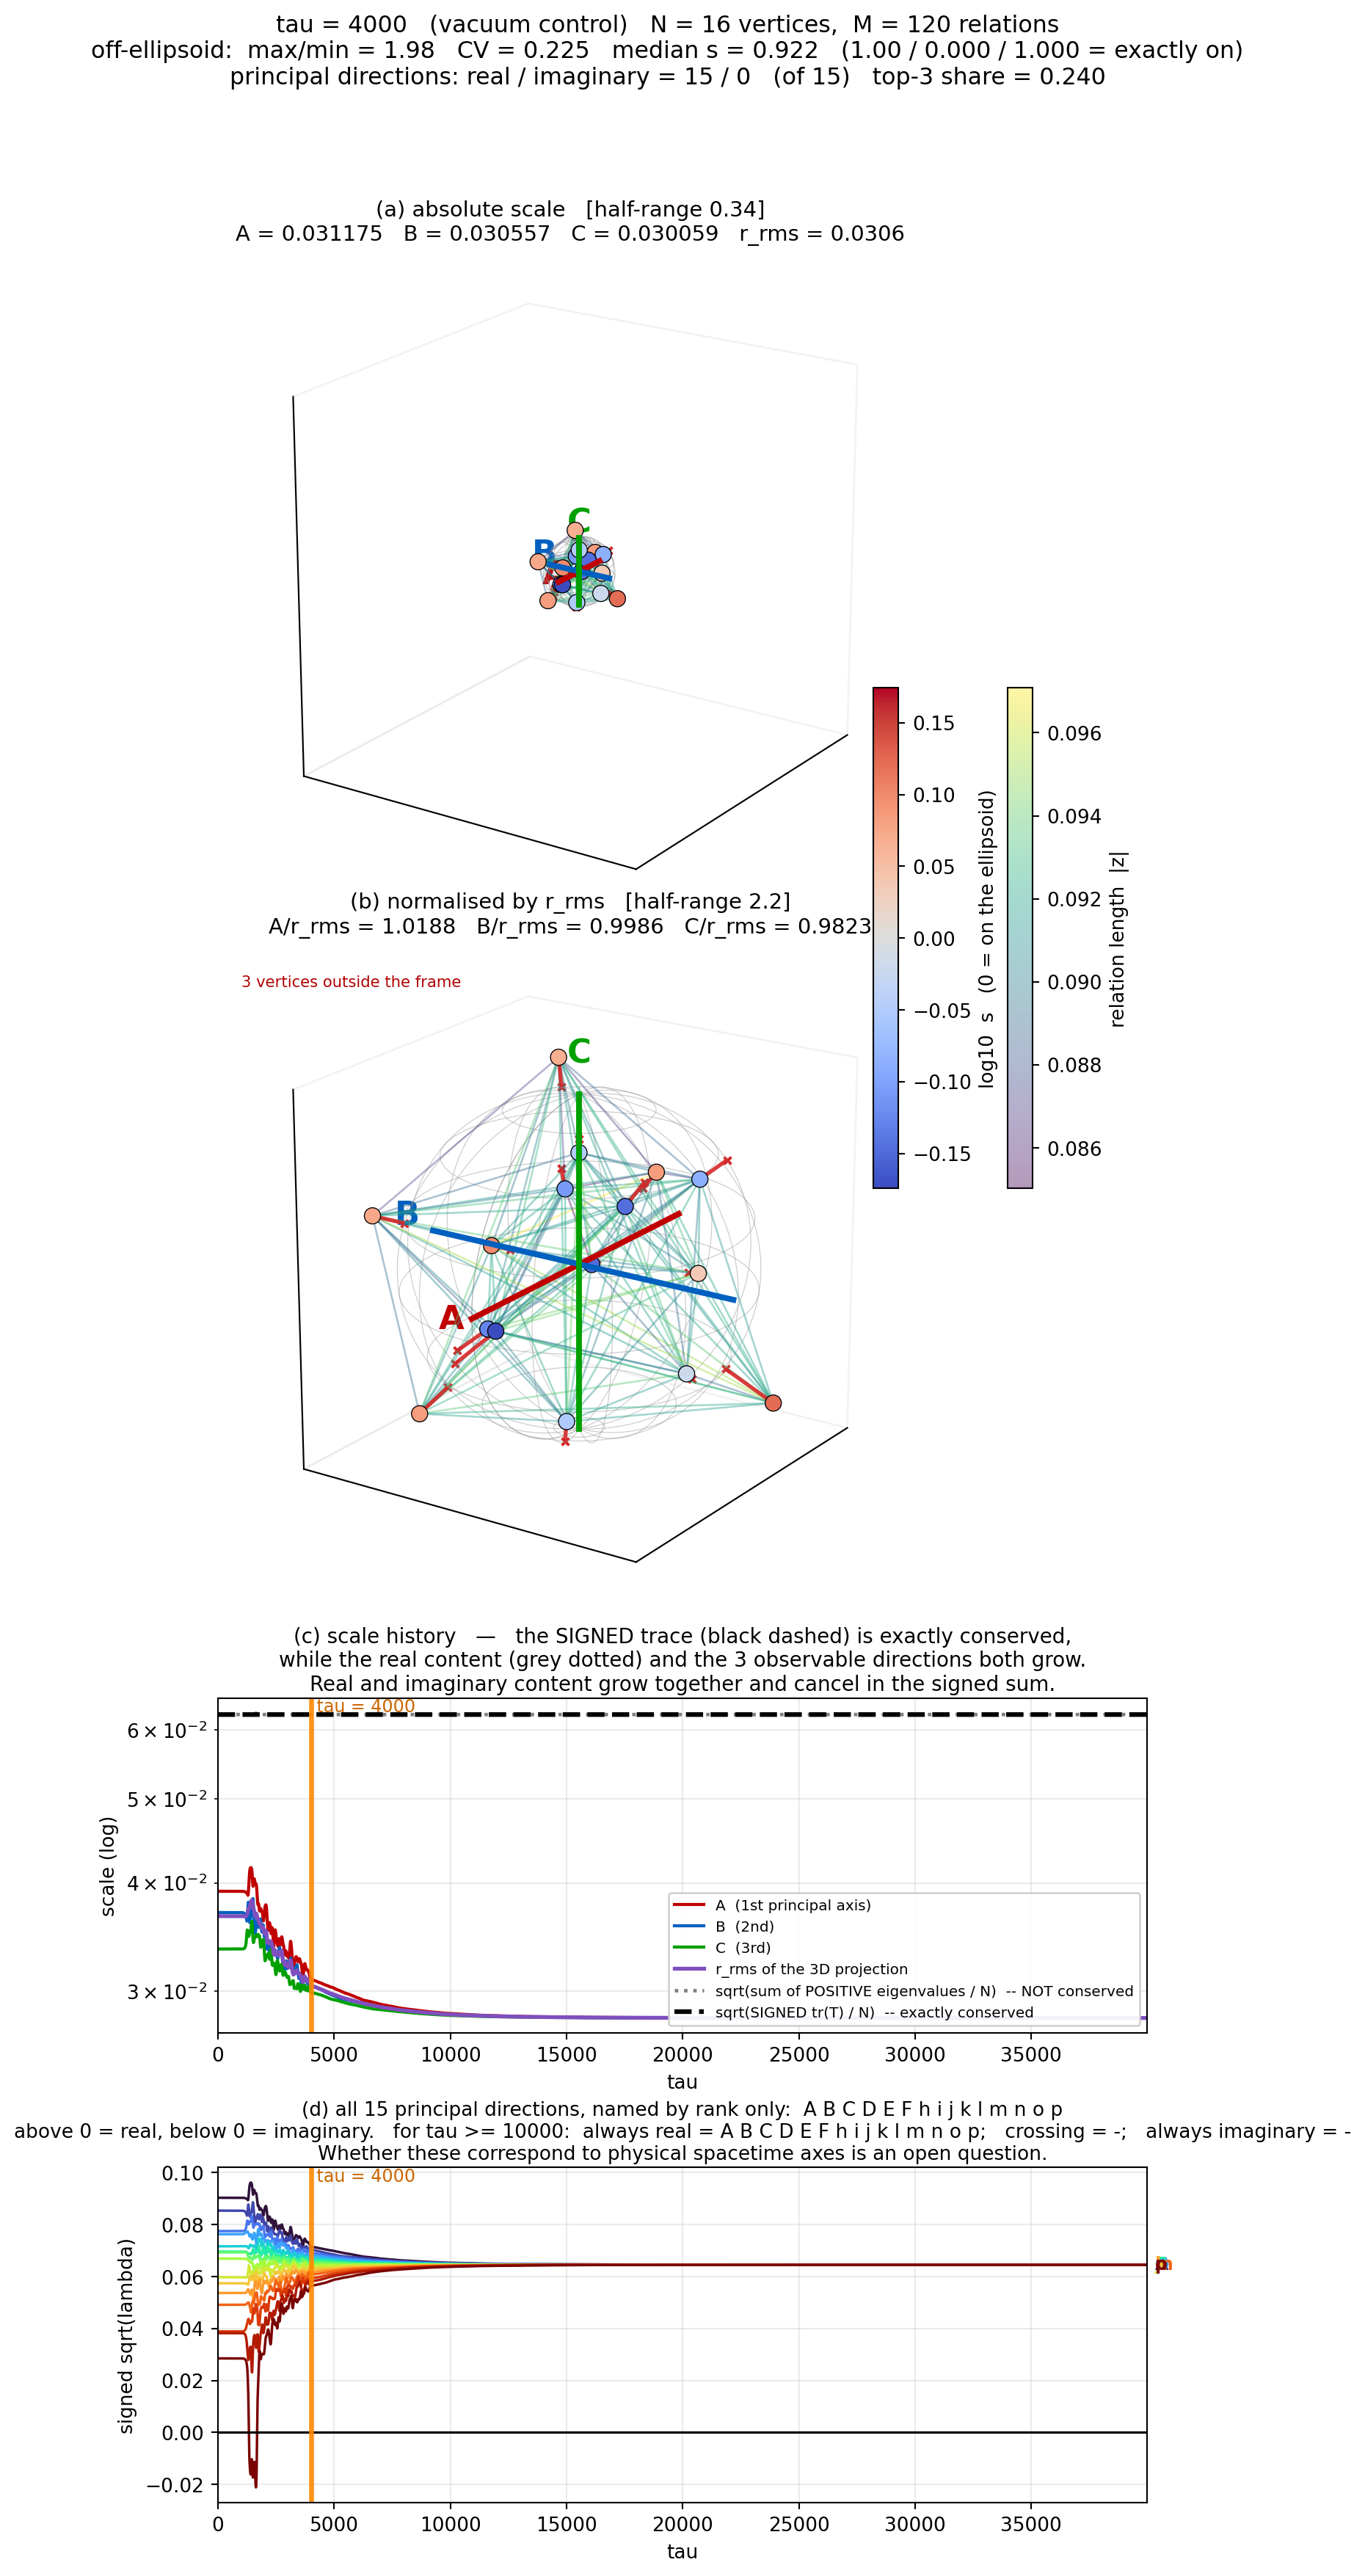
\includegraphics[keepaspectratio,alt={vacuum τ=4000}]{複製_ダンプ版_v1/次元の生成構造/対照実験_N掃引1to20_三系_v2/figures_tau/fig_ellipsoid_tau04000_electron_T40000_d0.1_rep-dump40k16_N16_v_v1.png}} \\
9487 &
\pandocbounded{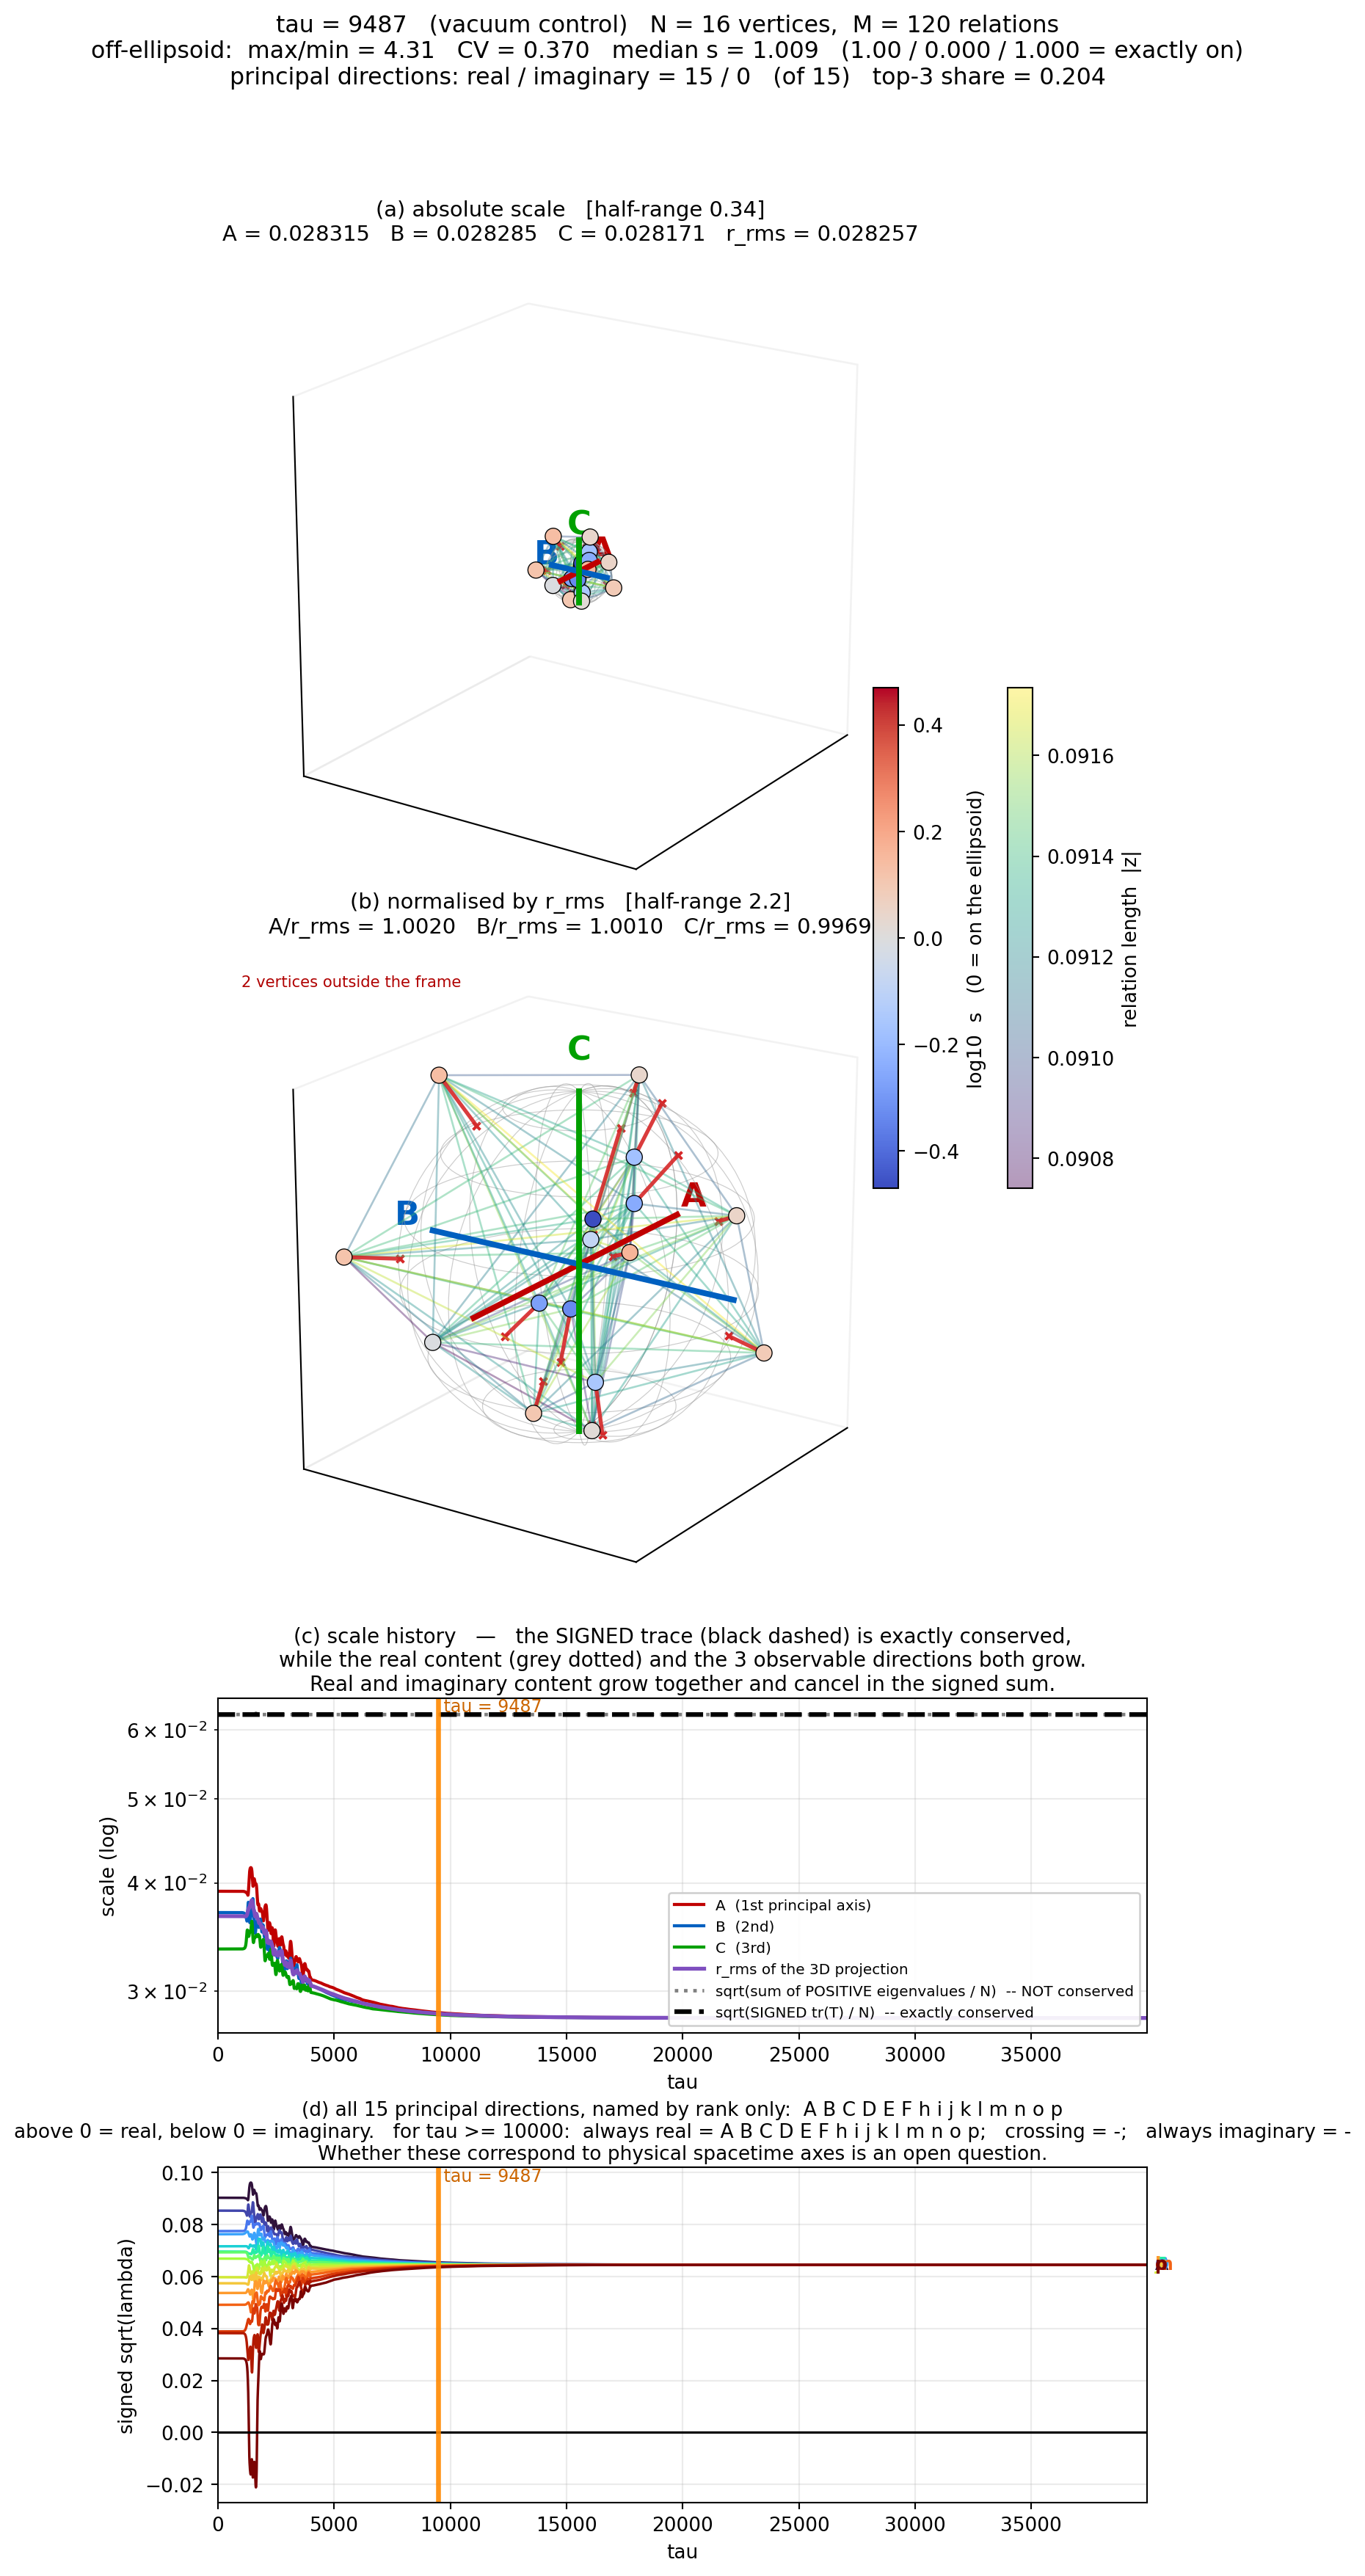
\includegraphics[keepaspectratio,alt={vacuum τ=9487}]{複製_ダンプ版_v1/次元の生成構造/対照実験_N掃引1to20_三系_v2/figures_tau/fig_ellipsoid_tau09487_electron_T40000_d0.1_rep-dump40k16_N16_v_v1.png}} \\
39991 &
\pandocbounded{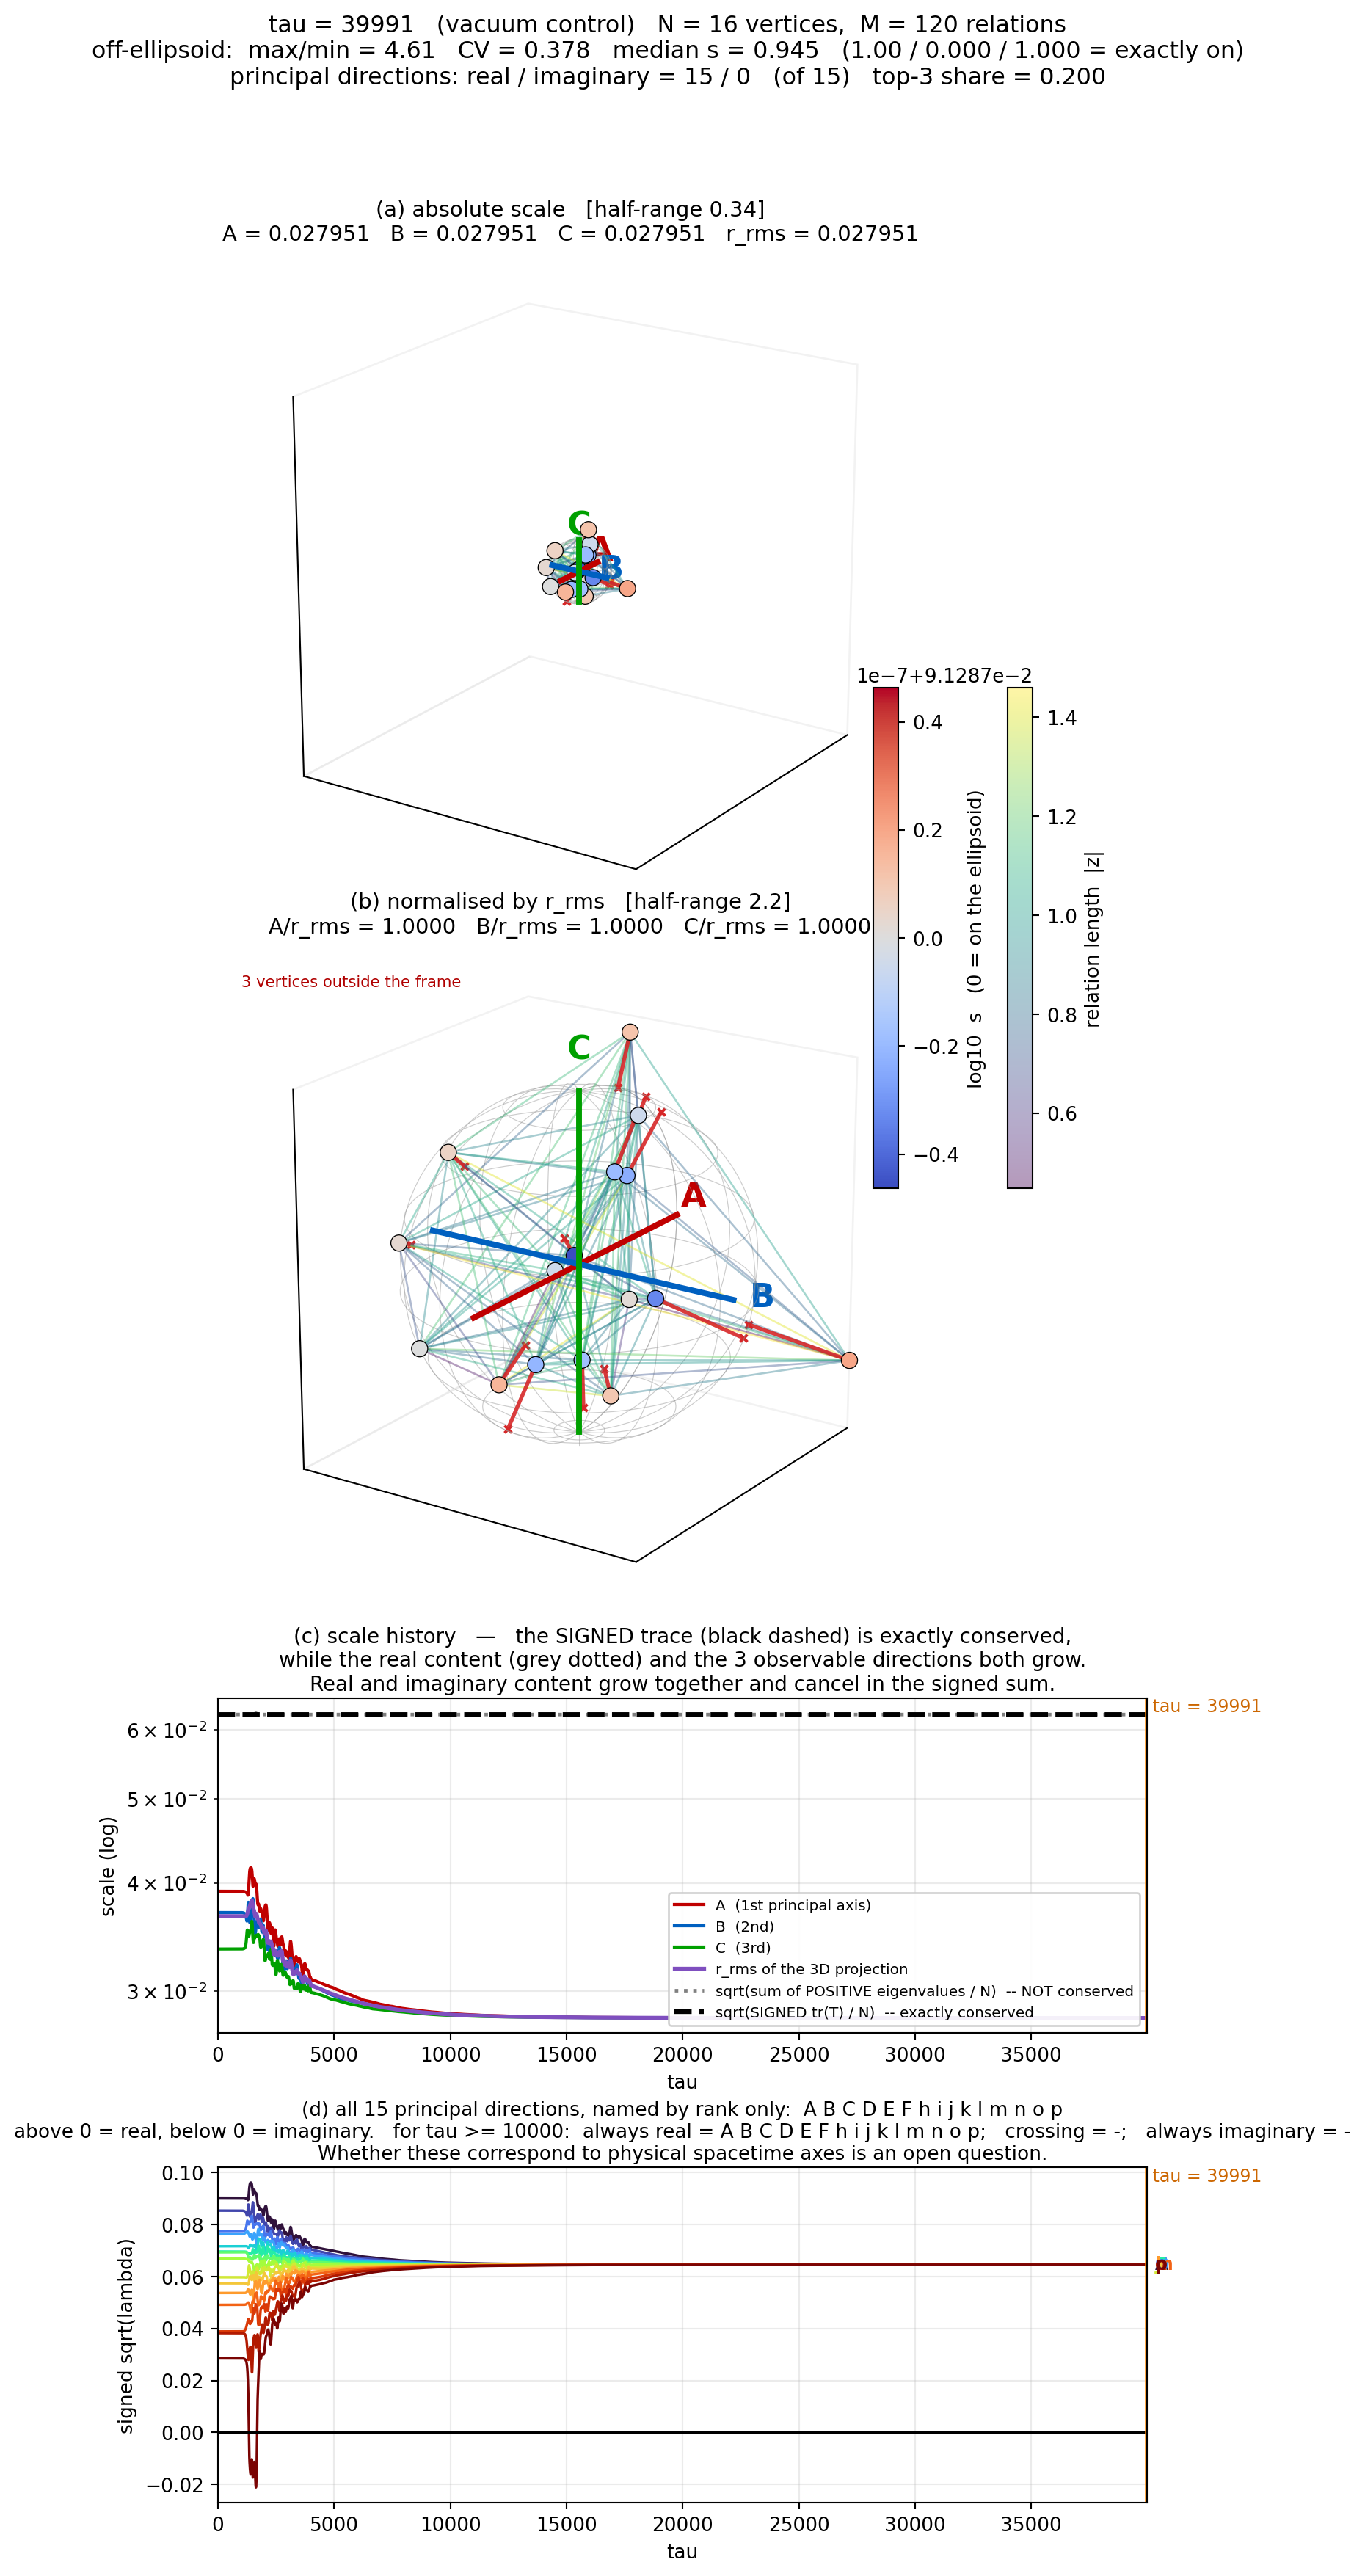
\includegraphics[keepaspectratio,alt={vacuum τ=39991}]{複製_ダンプ版_v1/次元の生成構造/対照実験_N掃引1to20_三系_v2/figures_tau/fig_ellipsoid_tau39991_electron_T40000_d0.1_rep-dump40k16_N16_v_v1.png}} \\
\end{longtable}
}

\begin{center}\rule{0.5\linewidth}{0.5pt}\end{center}

\subsection{5.3 How to read the figures, part 1 --- preventing
misreadings of the
inflation}\label{how-to-read-the-figures-part-1-preventing-misreadings-of-the-inflation}

\textbf{This section is required reading. Figures 5--8 invite two
opposite misreadings. Both are wrong.}

\subsubsection{Misreading 1: ``A conservation law holds, so no expansion
is
occurring''}\label{misreading-1-a-conservation-law-holds-so-no-expansion-is-occurring}

The \textbf{black dashed line} in panel (c) is perfectly horizontal over
all \(\tau\). Reading this as ``nothing is expanding'' is wrong.

The black dashed line represents the \textbf{signed} trace
\(\mathrm{tr}(B) = \sum_a\lambda_a\) (\(B\) the double-centred Gram
matrix, not the inertia tensor \(T\); see the notational caution in
Claim 5). By Lagrange's identity
\(\sum_{i<j}d_{ij}^2 = N\,\mathrm{tr}(B)\) this is the power of the
relation quantities itself. In measurement, the minimum and maximum over
the 968 late points agree to 8 digits (relative width
\(8.3\times10^{-9}\)). \textbf{This is conservation within numerical
precision, not an analytic conservation law derived from the update
rule} (the classification of Claim 13).

But \textbf{conservation of the signed sum does not mean that each
direction is still.}

The \textbf{grey dotted line} in the same panel (c) is the sum of the
positive eigenvalues alone. It is not horizontal; it jumps by \(1.90\)
at the transition. The absolute sum \(\sum_a|\lambda_a|\) grows by
\(2.79\). The real total grows, the imaginary total appears from near
zero, and their \textbf{difference} is conserved (Claim 13).

The exponential amplification is real. It is the red, blue and green
lines in panel (c) shooting up vertically at \(\tau\approx9000\).
\textbf{At \(N=12\) this jump was at \(\tau\approx2500\). The transition
time depends on the resolution.}

\subsubsection{\texorpdfstring{Misreading 2: ``\(A\) grew by \(2.8\), so
the whole system grew by
\(2.8\)''}{Misreading 2: ``A grew by 2.8, so the whole system grew by 2.8''}}\label{misreading-2-a-grew-by-2.8-so-the-whole-system-grew-by-2.8}

Also wrong. The signed trace does not move.

The three observed directions expand by the \textbf{product of two
effects}:

\begin{enumerate}
\def\labelenumi{\arabic{enumi}.}
\tightlist
\item
  the absolute sum grows by \(2.79\);
\item
  the top-3 occupancy rises from \(0.384\) to \(0.812\) (concentration).
\end{enumerate}

Neither alone explains it.

\subsubsection{Misreading 3: ``The extra dimensions
compactified''}\label{misreading-3-the-extra-dimensions-compactified}

\textbf{Also wrong.} \(m,n,o,p\) did not curl up small and vanish from
observation.

In panel (d), \(p\) \textbf{passes through} zero at \(\tau\approx9000\)
and continues down to \(-0.19\), \textbf{increasing in absolute value}.
The ratio across the transition is \(5.568\). Likewise \(o\) by
\(2.624\), \(n\) by \(1.674\), \(m\) by \(1.123\). \textbf{All four
directions moving to the imaginary side increase in absolute value.}
What shrinks are the alternating pair \(j\) (\(0.477\)) and \(k\)
(\(0.380\)).

So what is happening is not ``extra dimensions shrank'' but
\textbf{``three directions expanded and seven changed sign (three of
them alternating)''}. The mechanism is different.

\subsubsection{Misreading 4: ``There are 15 principal axes, so this
system is a 15-dimensional
parallelotope''}\label{misreading-4-there-are-15-principal-axes-so-this-system-is-a-15-dimensional-parallelotope}

\textbf{Also wrong.} The number of principal axes is \(N-1 = 15\), while
the parallelotope dimension required by zero closure is \(d=4\) (from
\(N=2^4\)); they are different (Claim 16-d). Had the system reached a
parallelotope, the rank would have to fall to \(4\), but the measured
rank is 8--11. It has not.

\subsubsection{Key points for reading the
figures}\label{key-points-for-reading-the-figures}

\begin{itemize}
\tightlist
\item
  Panel (a) has the frame fixed at \(\pm0.17\) for all \(\tau\). Placing
  the \(\tau=4000\) figure next to the \(\tau=39991\) figure shows
  directly that the ellipsoid itself has grown relative to the frame.
\item
  Panel (b) is divided by \(r_{\rm rms}\), so size information is
  removed and only shape remains. At \(\tau=39991\),
  \(A/r_{\rm rms}=1.230\) and \(C/r_{\rm rms}=0.529\): it has become
  oblate.
\item
  The vertical line in panel (c) is the current \(\tau\). Each figure's
  time point can be located there. \textbf{Do not judge the time series
  from the absolute scale of panel (a) alone.}
\item
  The letters at the right edge of panel (d) are the names of the 15
  principal axes.
\end{itemize}

\subsubsection{Comparison with the vacuum
control}\label{comparison-with-the-vacuum-control}

In Figures 9--12 (vacuum), \textbf{both} the black dashed and the grey
dotted lines in panel (c) are horizontal. No transition occurs, so the
absolute sum does not grow. The 15 lines in panel (d) all stay positive
and converge at \(\tau=39991\) to \(0.0645\), fully isotropic.

\textbf{The expansion and the fall into imaginary directions visible in
Figures 5--8 are phenomena accompanying the creation of matter, not
properties the system had from the outset.} That is the conclusion of
the control experiment.

\begin{center}\rule{0.5\linewidth}{0.5pt}\end{center}

\subsection{\texorpdfstring{5.4 How to read the figures, part 2 --- what
are the 15 principal axes
\(A,B,C,D,E,F,h,i,j,k,l,m,n,o,p\)?}{5.4 How to read the figures, part 2 --- what are the 15 principal axes A,B,C,D,E,F,h,i,j,k,l,m,n,o,p?}}\label{how-to-read-the-figures-part-2-what-are-the-15-principal-axes-abcdefhijklmnop}

\subsubsection{Why 15}\label{why-15}

A system of resolution \(N=16\) has \(M = N(N-1)/2 = 120\) relations.
Reading a length \(d_{ij}\) from each and forming the Gram matrix by
double centring

\[B = -\tfrac12\,J\,D^{\circ2}\,J,\qquad J = I - \tfrac1N\mathbf{1}\mathbf{1}^{\mathsf T}\]

gives \(B\mathbf{1} = 0\) exactly. That trivial zero is not a principal
axis, so there are \(N-1 = 15\) principal axes.

\textbf{The number 15 is \(N-1\) arising from the resolution \(N=16\),
not a number chosen from outside.} Changing \(N\) changes it (at
\(N=12\) it was 11). In this respect it differs in character from
dimension counts such as the \(10\) or \(11\) of superstring theory,
which are determined uniquely by consistency of the theory.

\textbf{And there is a ground for the choice of \(N\).} If zero closure
is realised as a parallelotope family then \(N=2^d\) (Claim 16), and
this note takes \(N=16=2^4\). Hence the number of principal axes is
\(2^d-1 = 15\). Do not confuse \(d\) with \(2^d-1\) (Claim 16-d).

\subsubsection{What the 15 do}\label{what-the-15-do}

{\def\LTcaptype{none} % do not increment counter
\begin{longtable}[]{@{}
  >{\raggedright\arraybackslash}p{(\linewidth - 8\tabcolsep) * \real{0.2000}}
  >{\raggedright\arraybackslash}p{(\linewidth - 8\tabcolsep) * \real{0.2000}}
  >{\raggedright\arraybackslash}p{(\linewidth - 8\tabcolsep) * \real{0.2000}}
  >{\raggedright\arraybackslash}p{(\linewidth - 8\tabcolsep) * \real{0.2000}}
  >{\raggedright\arraybackslash}p{(\linewidth - 8\tabcolsep) * \real{0.2000}}@{}}
\toprule\noalign{}
\begin{minipage}[b]{\linewidth}\raggedright
Group
\end{minipage} & \begin{minipage}[b]{\linewidth}\raggedright
Axes
\end{minipage} & \begin{minipage}[b]{\linewidth}\raggedright
ratio across the transition
\end{minipage} & \begin{minipage}[b]{\linewidth}\raggedright
real / imaginary
\end{minipage} & \begin{minipage}[b]{\linewidth}\raggedright
Role
\end{minipage} \\
\midrule\noalign{}
\endhead
\bottomrule\noalign{}
\endlastfoot
\textbf{\(A,B,C\)} & 1st--3rd & \(2.80\) / \(1.73\) / \(1.42\) & real &
\textbf{expand; appear in the three-dimensional projection; used for the
figures} \\
\textbf{\(D,E,F,h,i\)} & 4th--8th & \(1.27\) / \(1.14\) / \(1.01\) /
\(0.87\) / \(0.71\) & real & \textbf{nearly unchanged; real but absent
from the projection} \\
\textbf{\(j,k,l\)} & 9th--11th & \(0.48\) / \(0.38\) / \(0.73\) &
alternating & \textbf{cross the real/imaginary boundary; the cause of
the imaginary count fluctuating between 4 and 7} \\
\textbf{\(m,n,o,p\)} & 12th--15th & \(1.12\) / \(1.67\) / \(2.62\) /
\(5.57\) & imaginary & \textbf{fall to the imaginary side, but their
absolute values grow} \\
\end{longtable}
}

The real axes are the 8 from \(A\) to \(i\) and the imaginary ones the 4
\(m,n,o,p\), definitively; the 3 axes \(j,k,l\) cross back and forth.
``Six imaginary'' is the most frequent (616 of 968 points).

\subsubsection{What it means that the names are
ordinals}\label{what-it-means-that-the-names-are-ordinals}

The names \(A\) through \(p\) merely express the \textbf{rank order of
eigenvalues at that instant}. Note the following.

\begin{enumerate}
\def\labelenumi{\arabic{enumi}.}
\tightlist
\item
  \textbf{The names are not physical quantities.} No correspondence such
  as ``\(A\) is the time axis'' or ``\(B\) is \(R\)'' is claimed at all.
\item
  \textbf{The same name does not necessarily keep pointing in the same
  direction.} At times of eigenvalue degeneracy the order swaps. The
  measured minimum gap at \(N=16\) is
  \(3.4\times10^{-6}\)--\(5.1\times10^{-5}\), an order of magnitude
  smaller than at \(N=12\). Degeneracy really occurs.
\item
  \textbf{The principal-axis vectors are not continuous in time.} The
  absolute inner product of the first principal-axis vectors is only
  \(0.0450\) between \(\tau=4000\) and \(\tau=39991\), and \(0.0233\)
  between \(\tau=9487\) and \(\tau=39991\). The \(A\) just after the
  transition and the \(A\) at the end are nearly orthogonal, different
  directions.
\end{enumerate}

\textbf{Hence the 15 lines in panel (d) are not ``the time evolution of
15 physical axes''. They are the series of values ranked by eigenvalue
magnitude at each instant.} This distinction matters.

\subsubsection{Identification with physics is an open
task}\label{identification-with-physics-is-an-open-task}

We obtained a structure in which 3 of 15 directions expand rapidly, 5
stay nearly unchanged, and 7 move to imaginary (3 of them alternating).
However,

\begin{quote}
\textbf{whether these can be identified with physical spacetime (1 time
axis + 3 space axes, or \(R\) and \(Q\)), cannot be, or require an
intervening map, is an open task. There is at present no ground for
identification.}
\end{quote}

Likewise,

\begin{quote}
\textbf{how the spectral structure of these 15 principal axes relates to
superstring theory and other existing higher-dimensional theories is
also an open task.}
\end{quote}

\textbf{Up to v3 this note took \(N=12\), so there were 11 principal
axes, numerically matching the 11 dimensions of superstring theory. That
was an accident of the choice of resolution.} At \(N=16\) it becomes 15.
As stated in misreading 3 of §5.3, the mechanism also differs (this is
not compactification), and so does the provenance (\(N-1\) here,
consistency there). \textbf{A coincidence of words is not a
correspondence of theories.}

\begin{center}\rule{0.5\linewidth}{0.5pt}\end{center}

\subsection{5.5 Figure 13 --- the quasi-oscillation and its period
(Claim
15)}\label{figure-13-the-quasi-oscillation-and-its-period-claim-15}

\begin{figure}
\centering
\pandocbounded{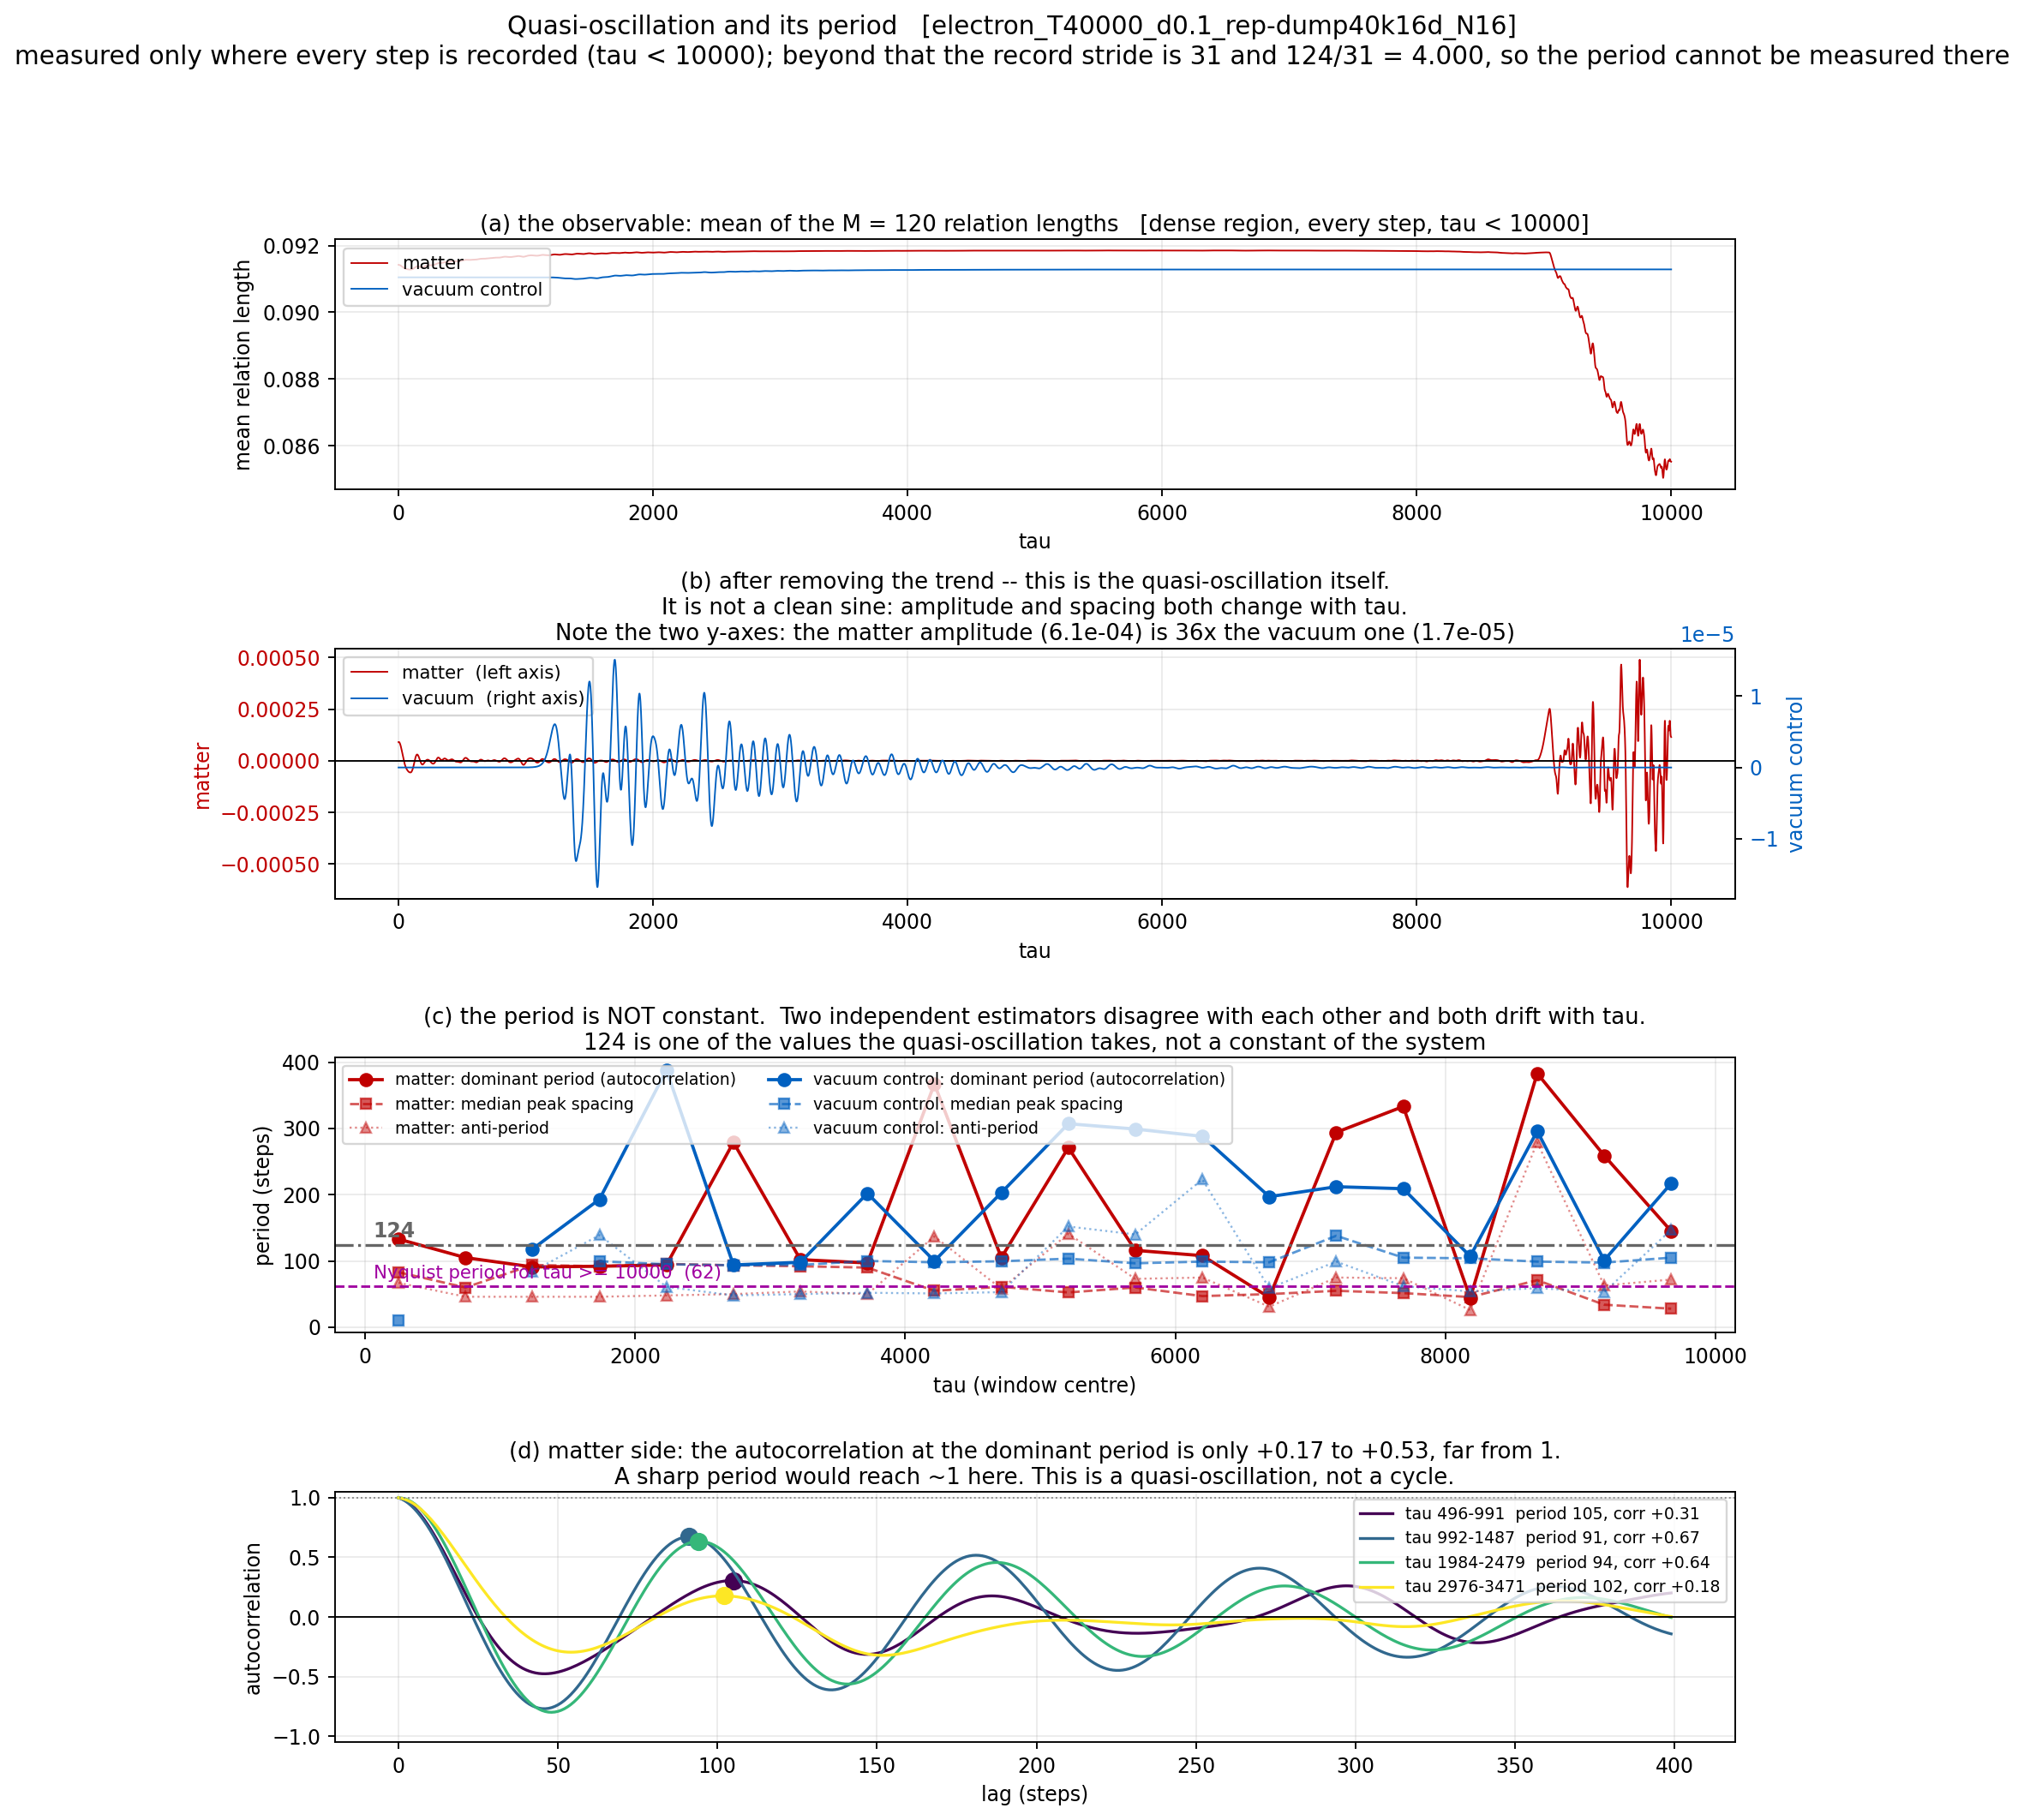
\includegraphics[keepaspectratio,alt={Figure 13}]{複製_ダンプ版_v1/次元の生成構造/対照実験_N掃引1to20_三系_v2/figures_tau/fig_period_electron_T40000_d0.1_rep-dump40k16d_N16_v1.png}}
\caption{Figure 13}
\end{figure}

The derivation program is
\texttt{複製\_ダンプ版\_v1/次元の生成構造/対照実験\_N掃引1to20\_三系\_v2/make\_period\_figure\_v1.py}.
The measured values themselves are stored in
\texttt{複製\_ダンプ版\_v1/次元の生成構造/対照実験\_N掃引1to20\_三系\_v2/figures\_tau/period\_series\_electron\_T40000\_d0.1\_rep-dump40k16d\_N16\_v1.npz}.

\textbf{This figure comes from the dedicated run with the dense region
widened to \(\tau<10000\) (\texttt{...rep-dump40k16d\_N16}) and includes
the transition (\(\tau\approx9000\)).} It shares conditions and random
seed with the ellipsoid-figure run \texttt{...rep-dump40k16\_N16},
differing only in the dense-region setting.

{\def\LTcaptype{none} % do not increment counter
\begin{longtable}[]{@{}
  >{\raggedright\arraybackslash}p{(\linewidth - 2\tabcolsep) * \real{0.5000}}
  >{\raggedright\arraybackslash}p{(\linewidth - 2\tabcolsep) * \real{0.5000}}@{}}
\toprule\noalign{}
\begin{minipage}[b]{\linewidth}\raggedright
Panel
\end{minipage} & \begin{minipage}[b]{\linewidth}\raggedright
Content
\end{minipage} \\
\midrule\noalign{}
\endhead
\bottomrule\noalign{}
\endlastfoot
(a) & the observable itself: the mean of the 120 relation lengths, dense
region only (every step recorded) \\
(b) & the residual after subtracting a 201-point moving average --- the
quasi-oscillation itself \\
(c) & \(\tau\) dependence of the dominant period: autocorrelation
(circles, solid), peak spacing (squares, dashed) and anti-period
(triangles, dotted) overlaid \\
(d) & the autocorrelations themselves; four matter-side windows \\
\end{longtable}
}

\textbf{How to read this figure}

\begin{itemize}
\tightlist
\item
  (a): the matter side (red) is flat until \(\tau\approx8900\) and then
  \textbf{falls sharply}. That is the transition. The vacuum side (blue)
  stays flat throughout. At \(N=12\) the same drop was at
  \(\tau\approx2300\).
\item
  (b): \textbf{the two sides use different axes.} The matter side (left
  axis) has almost zero amplitude until the transition, then rises
  abruptly from \(\tau\approx8900\). The vacuum side (right axis, order
  \(10^{-5}\)) shows one clean oscillation at
  \(\tau\approx1200\)--\(4000\) and then decays. \textbf{Before the
  transition there is an interval where the matter-side oscillation is
  in fact smaller than the vacuum side} (\(\tau\in[3968,8927]\), item 7
  of Claim 15). This panel is the basis for judging the peak spacings
  there to be noise.
\item
  (c): \textbf{this panel is the core of Claim 15.} The grey dash-dotted
  line is \(124\). Both estimation curves merely cross it and do not
  stay on it. \textbf{That the two estimators disagree with each other,
  and that both drift with \(\tau\), is the evidence that no single
  sharp period exists.} The purple dashed line is the Nyquist period
  \(62\) for \(\tau\ge10000\); below that line is unmeasurable in the
  late period. \textbf{The post-transition peak spacings \(34.0\to28.0\)
  lie below this line}, so they could not in principle be captured by
  the coarsely recorded run.
\item
  (d): \textbf{for a sharp period the autocorrelation at the dominant
  lag should reach \(1\).} The \(N=16\) measurements stay at
  \(+0.134\)--\(+0.673\) (the circles on each curve). This is the ground
  for judging it a ``quasi-oscillation'' rather than a ``cycle''. The
  shapes of the curves also differ per window.
\end{itemize}

\textbf{Misreadings this figure forbids}

\begin{quote}
``There is a period of \(124\) steps'' --- not accurate. \(124\) is one
value the quasi-oscillation takes, not a constant of the system. Note
that the two estimation curves in panel (c) do not sit on the \(124\)
line.

``There is a period, so \(U^n=I\) is confirmed'' --- not confirmed. If
it came from \(U^n=I\), the period would be a constant determined by
\(n\). The measurements vary. Whether it comes from \(U^n=I\) or from a
different phenomenon is unsettled.
\end{quote}

\begin{center}\rule{0.5\linewidth}{0.5pt}\end{center}

\subsection{6. What this note has
settled}\label{what-this-note-has-settled}

The answers to the two questions raised at the start are as follows.

\textbf{Question 1: Is representing waves by complex numbers
indispensable?}

It is not (Claim 9). What complex numbers add to the real indefinite
form is the single equation \(\sum q_np_n=0\) (Claim 8). \textbf{This
must not be called ``a restatement of scale symmetry''}, which would be
to return to the generator argument retracted in Claim 8.

\textbf{So the complex representation is not indispensable.} But
\textbf{the phrasing ``a convenient device saving one axiom'' is not
accurate}: reading A of axiom 0.5 can be removed from the independent
axioms because of the \textbf{homogeneity of the zero-closure equation},
not because of the complex representation (for a homogeneous equation
the solution set is a cone whether complex or not). \textbf{What the
complex representation adds to the real indefinite form is the
orthogonality condition \(\sum q_np_n=0\).}

\textbf{Question 2: What form does central projection take in the
complex representation?}

The centre of the central projection is not a vertex and is unobservable
from the subjective space. The imaginary symbol attaches only to the
direction of the centre, and all segment lengths remain real (Claim 7).

\textbf{And since assumption (S) holds in the central-projection
formulation (Claim 7), the structure ``the many-body problem reduces to
a single scalar equality constraint'' is preserved (Claim 0).} In the
real case, \(\sum x_n^2 = R^2\) represented an arbitrary point \(P\) on
the spherical shell of radius \(R\), and the constraint reduced to the
single \(X^{\mathsf T}F(X)=0\). In the complex case it becomes

\[x^2 + y^2 + z^2 - t^2 = R^2 + Q^2\]

which in four variables has signature \((3,1)\) --- a one-sheeted
hyperboloid, not closed. \textbf{Fixing the conserved quantity
\(C = t^2+R^2+Q^2\), and adding (U: the state lies in a
three-dimensional subspace) and (R: the readout is linear and regular,
\(X=\Lambda u\)), gives a closed surface (an ellipsoid) defined by
\(G=(\Lambda^{-1})^{\mathsf T}\Lambda^{-1}\)} (Claim 0-c).
\textbf{Fixing \(t\) alone does not close the surface, since \(C\)
changes if \(R,Q\) move.}

\textbf{The reduction itself holds with (S) alone and needs neither (U)
nor (R).} (U) and (R) are needed to relate it to observation
coordinates.

\textbf{Two things must not be confused, however.} First, a conserved
quantity does not determine the motion; it determines only \textbf{the
space of permitted motions}. Second, \textbf{that this ellipsoid is the
inertia ellipsoid itself is unproved}: that requires showing
\(G^{-1}\propto T\), which cannot be done while the readout map
\(\Lambda\) is not given (Claim 2B). \textbf{This is the largest
underived part of this note.}

\textbf{What is needed for the right-hand side to be conserved is
\(\dot C = 0\), and in the component layer of this model that can be
expected only for a steady solution.} In transient and metastable states
it deviates and may oscillate (Claims 0-d, 10, 15). The layer
distinction is also needed: those deviations are at the component layer,
while the readout layer has a quantity conserved through the transition
(Claims 18-c, 18-d).

As configurations satisfying zero closure in this form,
\textbf{parallelotopes} exist (Claim 4-b, valid for all \(d\)), with
vertex number \(N=2^d\). \textbf{That zero-closing configurations are
limited to parallelotopes is unproved for \(d\ge3\)} (Claim 4-e). That
centrally symmetric and convex is not enough was shown by
counterexamples (4-d). A parallelotope is always inscribed in an
ellipsoid, and its circumscribed ellipsoid coincides with the
\textbf{normalised inertia ellipsoid (\(c=d/N\))} (Claim 6B). The
second-order information of the configuration is exhausted by the
inertia ellipsoid and saturates at multipole \(l\le2\) (Claim 6).

That is, as an \textbf{exactly constructible family satisfying central
projection and zero closure simultaneously}, there are
\textbf{configurations built as the Minkowski sum of \(d\) segments,
inscribed in a single ellipsoid, whose ellipsoid information saturates
at \(l\le2\)}. \textbf{Whether it is the only such family is unproved}
(Claim 4-e).

\textbf{Question 3, added in v3: does the numerical model actually
become that configuration?}

It does not.

\begin{itemize}
\tightlist
\item
  \textbf{At the component layer}, zero closure is an identity holding
  only in the steady state and is violated in transient and metastable
  states. The deviation from the ellipsoid does not decrease
  monotonically in \(\tau\) and stays around max/min \(=12\) for 36,000
  steps after the transition (Claim 10).
\item
  This deviation depends on the seed strength; the \(\delta=0.1\) of
  this run is large. \textbf{Whether the deviation decreases with a
  weaker seed or a longer \(\tau\) is unverified} (Claim 11).
\item
  The configuration does not reach a parallelotope. The rank falls from
  \(15\) to \(8\)--\(11\) but not to \(d=4\) (§3B).
\item
  The double-centring readout has \(N-1=15\) non-trivial principal axes,
  and spectral concentration into the top three \(A,B,C\) magnifies the
  observed scale. \(D\)--\(i\) are nearly unchanged, \(m,n,o,p\) move to
  imaginary, and \(j,k,l\) alternate. \textbf{That this is not a
  compactification of the ``extra directions shrink and become
  invisible'' type} is established, but \textbf{identification with
  physical spacetime is an open task with no supporting ground} (Claim
  12).
\item
  If zero closure is realised as a parallelotope family, the resolution
  becomes \(N=2^d\); this note takes \(N=16\) (\(d=4\)). This is not a
  sufficient condition (rank \(=d\) alone is also insufficient), and it
  is not derived that it is necessary for all zero-closing solutions
  (Claim 16).
\item
  What selects parallelotopes is not the form of the equation
  \(\sum x_n^2=0\) but the face-dimension sign rule. If both signs and
  configuration may be chosen freely, non-trivial solutions exist from
  \(N\ge3\) (Claim 17).
\item
  What is conserved is the signed trace; the real and imaginary totals
  both grow and cancel (Claim 13).
\item
  Imaginary directions do not exist in the vacuum and appear with the
  creation of matter (Claim 14).
\item
  \textbf{The orientation of the principal axes is not conserved.} The
  top-3 subspace loses correlation to the random level in about 2000
  steps and does not stabilise over a \(36{,}000\)-step sweep. But
  \textbf{orientation-independent conserved quantities (quadratic forms)
  do exist}: at least the two kinds \(\sum_e\lvert x_e\rvert^2\) and
  \(\sum_e x_e^2\), both of trace type and hence unaffected by the
  diffusion of orientation. In particular \(\sum_e x_e^2\) is
  \textbf{invariant as a complex number through the transition} (Claim
  18).
\item
  Quasi-oscillations of order \(10^2\) steps exist, but the period
  varies with \(\tau\). At \(N=16\) the pre-transition peak spacing
  \(90\)--\(95.5\) shortens to \(34.0\) in the transition window and
  \(28.0\) just after, while the vacuum side stays at \(93.5\)--\(138\)
  and does not shorten. \textbf{The \(N=12\) finding that the transition
  shortens the period was reproduced at \(N=16\).} \textbf{Whether this
  is due to the second axiom \(U^n=I\) or a different phenomenon is an
  open task} (Claim 15).
\end{itemize}

\textbf{Question 4, added in v4: what are the title's ``four
dimensions''?}

They are the \textbf{four dimensions} with coordinates \((r,t,R,Q)\)
(Claim 2B). And since zero closure gives

\[r^2 = t^2 + R^2 + Q^2,\]

there is a \textbf{light-cone-type null cone} inside that
four-dimensional space. \textbf{That is the meaning of the title.}

\(x,y,z\) belong to the subsequent three-dimensional readout and are not
needed for the four-dimension claim. Relationality gives only the length
\(r\), and \(x,y,z\) are points on the surface \(S_r^2\) that \(r\)
permits (Claim 2B). The degrees of freedom on the null cone are 3;
projectivised, 2.

\textbf{This is a different object from the parallelotope dimension
\(d=4\) (\(N=16\), Claim 16). The numerical coincidence is accidental
and neither follows from the other.}

\textbf{Question 5, added in v4: does the orientation stabilise?}

It does not (Claim 18-a). But \textbf{what matters is not the
orientation but whether orientation-independent conserved quantities
(quadratic forms) exist.} They do (Claim 18-b): at least the Hermitian
\(\sum\lvert x_e\rvert^2\) and the bilinear \(\sum x_e^2\), the latter
invariant as a complex number through the transition. Both are of trace
type, so their values do not change as the orientation diffuses.
\textbf{However, conservation holds only at the readout layer, not at
the component layer (Claim 18-d).}

This result organises the two unresolved items --- the readout map from
\(r\) (Claim 2B) and the identification of \(A,B,\dots,p\) with physics
(Claim 12) --- as \textbf{one and the same problem}. \textbf{Within this
run}, identification with a fixed frame is not supported, and if
anything can be identified it is orientation-independent quantities
(Claim 18-f).

\textbf{A distance remains unbridged between the geometric statements
(Claims 1--9) and the measurements on the numerical model (Claims
10--18).} This note measured that distance and identified where it is
unbridged. The work needed to bridge it narrows to the following five
items.

\begin{enumerate}
\def\labelenumi{\arabic{enumi}.}
\tightlist
\item
  \textbf{Establish assumption (S) on the model side, or show that it
  does not hold} (Claim 0-b). If the supports of the real and imaginary
  parts separate, the orthogonality condition \(\sum q_np_n=0\) becomes
  an identity and the independent constraints drop from two to
  \textbf{one}. \textbf{If this goes through, the central claim of this
  note --- reducing the many-body problem to a single quadratic equality
  constraint --- is completed on the model side as well. This is the top
  priority.}
\item
  \textbf{Establish assumption (\(\Gamma\): geometric sign
  correspondence), or show that it does not hold} (Claim 5, §3B):
  whether the partition \(\mathcal{I}_\pm\) coincides with the partition
  by the face-dimension sign \(s_e\). \textbf{Until this goes through,
  complex zero closure and the signed closure \(S(D)=0\) of Claim 4 are
  not connected.}
\item
  \textbf{Show the existence of the three-dimensional state subspace
  \(U\), give the readout map \(\Lambda\), and show \(G^{-1}\propto T\)}
  (Claim 0-c). All three are underived. If all go through, ``the readout
  surface of complex zero closure = the inertia ellipsoid'' connects in
  one line and Claim 0 links directly to Claim 6B.
\item
  \textbf{Derive from the update rule an identity corresponding to
  \(X^{\mathsf T}F(X)=\tfrac12\dot C\)} (Claims 13, 18-b). The present
  conservation is an observation within numerical precision, not an
  analytic conservation law.
\item
  \textbf{Prove ``zero closure \(\Rightarrow\) parallelotope'' for
  \(d\ge3\), or produce a counterexample} (Claim 4-e). Until this is
  settled, \(N=2^d\) remains a conditional statement.
\end{enumerate}

\begin{center}\rule{0.5\linewidth}{0.5pt}\end{center}

\subsection{Appendix A. List of programs used in this
note}\label{appendix-a.-list-of-programs-used-in-this-note}

All are stored in the repository. \textbf{Paths are relative to the
location of this file, written without abbreviation.} Hashes are the
first 8 hex digits of the MD5.

There are two replicas.

\begin{itemize}
\tightlist
\item
  \texttt{複製\_対照実験\_N16\_v1/} --- verified replica, copied from
  the originals with matching md5, \textbf{not modified by a single
  line}.
\item
  \texttt{複製\_ダンプ版\_v1/} --- dump-modified version. \textbf{This
  is what was actually run.}
\end{itemize}

Since the dependencies use \texttt{HERE.parent} and
\texttt{PAPER8.parent.parent}, the replicas preserve the
repository-relative nesting. The internal relative structure is
identical in both, and the paths below are those of the
\texttt{複製\_ダンプ版\_v1/} side used for the runs.

\subsubsection{A.1 Programs newly written for this note
(7)}\label{a.1-programs-newly-written-for-this-note-7}

{\def\LTcaptype{none} % do not increment counter
\begin{longtable}[]{@{}
  >{\raggedright\arraybackslash}p{(\linewidth - 6\tabcolsep) * \real{0.2500}}
  >{\raggedright\arraybackslash}p{(\linewidth - 6\tabcolsep) * \real{0.2500}}
  >{\raggedright\arraybackslash}p{(\linewidth - 6\tabcolsep) * \real{0.2500}}
  >{\raggedright\arraybackslash}p{(\linewidth - 6\tabcolsep) * \real{0.2500}}@{}}
\toprule\noalign{}
\begin{minipage}[b]{\linewidth}\raggedright
File
\end{minipage} & \begin{minipage}[b]{\linewidth}\raggedright
Hash
\end{minipage} & \begin{minipage}[b]{\linewidth}\raggedright
Role
\end{minipage} & \begin{minipage}[b]{\linewidth}\raggedright
Products
\end{minipage} \\
\midrule\noalign{}
\endhead
\bottomrule\noalign{}
\endlastfoot
\texttt{複製\_ダンプ版\_v1/次元の生成構造/対照実験\_N掃引1to20\_三系\_v2/make\_scale\_series\_v1.py}
& \texttt{4df6b80c} & extracts and caches, from the dump, the
principal-axis spectrum, rank, imaginary-direction count, signed trace,
and positive/negative parts at all \(\tau\) &
\texttt{複製\_ダンプ版\_v1/次元の生成構造/対照実験\_N掃引1to20\_三系\_v2/scale\_series\_*.npz} \\
\texttt{複製\_ダンプ版\_v1/次元の生成構造/対照実験\_N掃引1to20\_三系\_v2/make\_ellipsoid\_figure\_v1.py}
& \texttt{2f75f478} & the four-panel figure at a given \(\tau\)
(ellipsoid, normalised, scale history, all \(N-1\) principal-axis
histories). Derivation of Claims 10, 12, 13, 14. \textbf{Extended in v4
to 15 axis names (\(\dots l,m,n,o,p\))} (the v3 hash was
\texttt{da11c229}, which had names only up to 11 and drew the 12th
onward by number) & Figures 5--12 \\
\texttt{複製\_ダンプ版\_v1/次元の生成構造/対照実験\_N掃引1to20\_三系\_v2/make\_period\_figure\_v1.py}
& \texttt{5ea24de2} & measures the quasi-oscillation period by both
autocorrelation and peak spacing and plots it. Derivation of Claim 15.
\textbf{Two fixes in v4} (v3 hash \texttt{a384c970}): (1) the
dense-region end \texttt{-\/-dense-end} was fixed at 4000, a trap by
which even a widened dense run measured only \(\tau<4000\); the default
is now read from \texttt{dump\_tauc} in \texttt{dump\_meta}. (2) the
title of panel (a) was fixed at \texttt{M\ =\ 66}, wrong for \(N=16\)
(\(M=120\)); it is now read from \texttt{m} in the meta & Figure 13,
\texttt{複製\_ダンプ版\_v1/次元の生成構造/対照実験\_N掃引1to20\_三系\_v2/figures\_tau/period\_series\_*.npz} \\
\texttt{複製\_ダンプ版\_v1/次元の生成構造/対照実験\_N掃引1to20\_三系\_v2/check\_invariants\_v1.py}
& \texttt{a9f78842} & measures the stability of principal-axis
orientation (subspace overlap) and the conserved quadratic invariants
(Hermitian, bilinear, \(\mathrm{tr}(B^k)\), component layer). Derivation
of Claim 18 & \texttt{figures\_tau/invariants\_*.json} \\
\texttt{figures\_v1/make\_figs.py} & \texttt{7fc0ac70} & face-dimension
classification of parallelotopes (\(d=3\) and \(d=4\)). Derivation of
Claim 4 & Figures 1, 2 \\
\texttt{figures\_v1/make\_fig3.py} & \texttt{ff721504} & contrast of
centrally symmetric convex counterexamples (icosahedron, octahedron)
with a parallelotope. Derivation of Claim 4-d & Figure 3 \\
\texttt{figures\_v1/make\_fig4.py} & \texttt{b940a9af} & the
zero-closure ellipsoid, semi-axes \(A,B,C\), and the degrees of freedom
closure fixes. Derivation of Claims 5, 6, 6B & Figure 4 \\
\texttt{figures\_v1/check\_sufficiency\_v1.py} & \texttt{eb58bbef} &
that \(N=2^d\) and rank \(=d\) are insufficient singly and jointly, the
trivialisation of the test at rank \(=N-1\), and the degeneracy at
\(N=d+1\) (simplex). Derivation of Claims 16-b, 16-c &
\texttt{check\_sufficiency\_v1.json} \\
\texttt{figures\_v1/check\_real\_solutions\_v1.py} & \texttt{c45e9259} &
that sign choice alone cannot zero a fixed distance set and that it is
solvable when both signs and configuration are free (test B),
\(\sum_{\text{edges}}d^2 = \sum_{\text{main diagonals}}d^2\) (test D),
the real/imaginary breakdown by face-dimension class (test E), and class
recovery from lengths alone (test F). Derivation of Claims 4-f, 4-g, 17
& \texttt{check\_real\_solutions\_v1.json} \\
\end{longtable}
}

\subsubsection{A.2 Run programs --- modified
(2)}\label{a.2-run-programs-modified-2}

The originals (on the \texttt{複製\_対照実験\_N16\_v1/} side) are not
rewritten by a single line. Modifications were made only on the
\texttt{複製\_ダンプ版\_v1/} side and are marked in place. The hashes
are those before modification (the originals).

{\def\LTcaptype{none} % do not increment counter
\begin{longtable}[]{@{}
  >{\raggedright\arraybackslash}p{(\linewidth - 4\tabcolsep) * \real{0.3333}}
  >{\raggedright\arraybackslash}p{(\linewidth - 4\tabcolsep) * \real{0.3333}}
  >{\raggedright\arraybackslash}p{(\linewidth - 4\tabcolsep) * \real{0.3333}}@{}}
\toprule\noalign{}
\begin{minipage}[b]{\linewidth}\raggedright
File
(\texttt{複製\_ダンプ版\_v1/次元の生成構造/対照実験\_N掃引1to20\_三系\_v2/})
\end{minipage} & \begin{minipage}[b]{\linewidth}\raggedright
hash of \texttt{R}
\end{minipage} & \begin{minipage}[b]{\linewidth}\raggedright
Modification
\end{minipage} \\
\midrule\noalign{}
\endhead
\bottomrule\noalign{}
\endlastfoot
\texttt{run\_nsweep\_three\_series\_v2.py} & \texttt{3e8e06c8} & added a
two-stage sampling dump: every step up to \texttt{DUMP\_TAUC} (default
4000), thereafter every \texttt{DUMP\_STRIDE} (default 31), writing
\(C_2\) to a memmap. The correspondence table \texttt{dump\_taus} is
saved in the meta. The physics, recorded items, decision logic and
figure generation are untouched \\
\texttt{run\_tb\_nsweep\_1to20\_v1.py} & \texttt{bfa5d854} & added a
path saving the final-frame diagnostic dictionary as per-key arrays \\
\end{longtable}
}

\subsubsection{A.3 Run programs --- unmodified
(22)}\label{a.3-run-programs-unmodified-22}

Byte-identical between \texttt{複製\_対照実験\_N16\_v1/} and
\texttt{複製\_ダンプ版\_v1/}. These are what determine the physics.

\textbf{Core (unified universal functions)}

{\def\LTcaptype{none} % do not increment counter
\begin{longtable}[]{@{}ll@{}}
\toprule\noalign{}
File (\texttt{複製\_ダンプ版\_v1/次元の生成構造/統一万能関数\_v1/}) &
Hash \\
\midrule\noalign{}
\endhead
\bottomrule\noalign{}
\endlastfoot
\texttt{unified\_interaction\_v1.py} & \texttt{bf45d4c7} \\
\texttt{unified\_interaction\_v2.py} & \texttt{728e79a7} \\
\texttt{unified\_readout\_v3.py} & \texttt{bea700fe} \\
\texttt{unified\_dimension\_v1.py} & \texttt{1416d9ad} \\
\texttt{selection\_v1.py} & \texttt{5c23ced4} \\
\end{longtable}
}

\textbf{Universal inelastic map, many-body connection, parent white
wave}

{\def\LTcaptype{none} % do not increment counter
\begin{longtable}[]{@{}
  >{\raggedright\arraybackslash}p{(\linewidth - 2\tabcolsep) * \real{0.5000}}
  >{\raggedright\arraybackslash}p{(\linewidth - 2\tabcolsep) * \real{0.5000}}@{}}
\toprule\noalign{}
\begin{minipage}[b]{\linewidth}\raggedright
File
\end{minipage} & \begin{minipage}[b]{\linewidth}\raggedright
Hash
\end{minipage} \\
\midrule\noalign{}
\endhead
\bottomrule\noalign{}
\endlastfoot
\texttt{複製\_ダンプ版\_v1/次元の生成構造/万能非弾性写像\_managed\_v1/universal\_inelastic\_map\_v1.py}
& \texttt{7c07a52e} \\
\texttt{複製\_ダンプ版\_v1/次元の生成構造/万能非弾性写像\_managed\_v1/universal\_inelastic\_map\_v3.py}
& \texttt{bfb15801} \\
\texttt{複製\_ダンプ版\_v1/次元の生成構造/万能非弾性写像\_managed\_v1/run\_ignition\_fate\_exact\_v3.py}
& \texttt{a95f3327} \\
\texttt{複製\_ダンプ版\_v1/次元の生成構造/万能相互作用多体接続\_v1/run\_stage2\_vertex\_engine\_v1.py}
& \texttt{55f88e26} \\
\texttt{複製\_ダンプ版\_v1/次元の生成構造/万能相互作用多体接続\_v1/run\_stage3\_sharedO\_v2\_and\_hair\_v1.py}
& \texttt{75bc31db} \\
\texttt{複製\_ダンプ版\_v1/次元の生成構造/make\_parent\_white\_managed\_v1/make\_parent\_white\_harmonics\_n\_only\_v3.py}
& \texttt{328c0457} \\
\end{longtable}
}

\textbf{Run environments of earlier papers (loaded as dependencies)}

{\def\LTcaptype{none} % do not increment counter
\begin{longtable}[]{@{}
  >{\raggedright\arraybackslash}p{(\linewidth - 2\tabcolsep) * \real{0.5000}}
  >{\raggedright\arraybackslash}p{(\linewidth - 2\tabcolsep) * \real{0.5000}}@{}}
\toprule\noalign{}
\begin{minipage}[b]{\linewidth}\raggedright
File
\end{minipage} & \begin{minipage}[b]{\linewidth}\raggedright
Hash
\end{minipage} \\
\midrule\noalign{}
\endhead
\bottomrule\noalign{}
\endlastfoot
\texttt{複製\_ダンプ版\_v1/次元の生成構造/第8論文\_二段階seed除去による準安定相の因果分離/code/run\_preliminary\_seed\_ablation\_v1.py}
& \texttt{45c4b42a} \\
\texttt{複製\_ダンプ版\_v1/次元の生成構造/第9論文\_フェルミオンの生成構造/対照実験\_波束収縮\_実行環境\_v1/20260713/run\_exchange\_scattering\_matrix\_fermionic\_localization\_transfer\_preliminary\_v1.py}
& \texttt{3cb0bfda} \\
\texttt{複製\_ダンプ版\_v1/次元の生成構造/第9論文\_フェルミオンの生成構造/対照実験\_波束収縮\_実行環境\_v1/20260715/run\_system\_A\_localization\_exchange\_R\_sweep\_preliminary\_v1.py}
& \texttt{941c7b21} \\
\texttt{複製\_ダンプ版\_v1/次元の生成構造/第9論文\_フェルミオンの生成構造/対照実験\_波束収縮\_実行環境\_v1/ab\_invariant\_theta\_toy\_v1/run\_ab\_invariant\_theta\_toy\_v1.py}
& \texttt{682a41ce} \\
\texttt{複製\_ダンプ版\_v1/時間軸Q軸とフェルミオンの生成構造/検証\_対照実験/第5論文原本\_自発的分裂予備実験\_v1/run\_n\_scaling\_lowrank\_v1.py}
& \texttt{1b63c1ec} \\
\texttt{複製\_ダンプ版\_v1/時間軸Q軸とフェルミオンの生成構造/検証\_対照実験/第5論文原本\_自発的分裂予備実験\_v1/run\_plane\_flow\_exact\_v1.py}
& \texttt{444ea69f} \\
\texttt{複製\_ダンプ版\_v1/時間軸Q軸とフェルミオンの生成構造/検証\_対照実験/第5論文原本\_自発的分裂予備実験\_v1/run\_plane\_flow\_approx\_v1.py}
& \texttt{5d6a5e8a} \\
\texttt{複製\_ダンプ版\_v1/時間軸Q軸とフェルミオンの生成構造/検証\_対照実験/第5論文原本\_自発的分裂予備実験\_v1/exact\_lowN\_eigenspectrum\_v2/code/run\_n300\_dimension\_saturation\_v2.py}
& \texttt{a11fb4ca} \\
\texttt{複製\_ダンプ版\_v1/時間軸Q軸とフェルミオンの生成構造/検証\_対照実験/第5論文原本\_自発的分裂予備実験\_v1/exact\_lowN\_eigenspectrum\_v2/paper7\_longtime/code/run\_paper7\_5color\_timeseries.py}
& \texttt{25b4dbde} \\
\texttt{複製\_ダンプ版\_v1/時間軸Q軸とフェルミオンの生成構造/検証\_対照実験/第5論文原本\_自発的分裂予備実験\_v1/exact\_lowN\_eigenspectrum\_v2/paper7\_longtime/code/run\_paper7\_transverse.py}
& \texttt{6c0125b5} \\
\end{longtable}
}

\textbf{Condition-fixing runner}

{\def\LTcaptype{none} % do not increment counter
\begin{longtable}[]{@{}
  >{\raggedright\arraybackslash}p{(\linewidth - 4\tabcolsep) * \real{0.3333}}
  >{\raggedright\arraybackslash}p{(\linewidth - 4\tabcolsep) * \real{0.3333}}
  >{\raggedright\arraybackslash}p{(\linewidth - 4\tabcolsep) * \real{0.3333}}@{}}
\toprule\noalign{}
\begin{minipage}[b]{\linewidth}\raggedright
File
\end{minipage} & \begin{minipage}[b]{\linewidth}\raggedright
Hash
\end{minipage} & \begin{minipage}[b]{\linewidth}\raggedright
Role
\end{minipage} \\
\midrule\noalign{}
\endhead
\bottomrule\noalign{}
\endlastfoot
\texttt{複製\_ダンプ版\_v1/次元の生成構造/対照実験\_N掃引1to20\_三系\_v2/run\_sample4fig\_electron\_N12\_d0.1\_T4000\_v1.py}
& \texttt{d86c535f} & a wrapper launching the unmodified original with
the conditions fixed. The ground for the choice of \(\delta\) level is
recorded in the docstring \\
\end{longtable}
}

\subsubsection{A.4 Reproduction
procedure}\label{a.4-reproduction-procedure}

\textbf{The starting directory is the one containing this file,
\texttt{次元の生成構造/ゼロ閉塞の幾何・代数構造/}.} The \texttt{cd}
below are relative to it.

\begin{Shaded}
\begin{Highlighting}[]
\CommentTok{\# 1. Run (N=16=2\^{}4, dumped with two{-}stage sampling)}
\BuiltInTok{cd}\NormalTok{ 複製\_ダンプ版\_v1/次元の生成構造/対照実験\_N掃引1to20\_三系\_v2}
\VariableTok{DUMP\_TAUC}\OperatorTok{=}\NormalTok{4000 }\VariableTok{DUMP\_STRIDE}\OperatorTok{=}\NormalTok{31 }\DataTypeTok{\textbackslash{}}
  \ExtensionTok{python3}\NormalTok{ run\_nsweep\_three\_series\_v2.py electron 16 16 40000 0.1 dump40k16}

\CommentTok{\# 2. Extract the principal{-}axis spectrum (matter and vacuum)}
\ExtensionTok{python3}\NormalTok{ make\_scale\_series\_v1.py electron\_T40000\_d0.1\_rep{-}dump40k16\_N16 m v}

\CommentTok{\# 3. Figures 5{-}12 (four time points x matter/vacuum)}
\CommentTok{\#    tau is chosen to match the N=16 transition (tau approx 9000{-}9500)}
\ControlFlowTok{for}\NormalTok{ side }\KeywordTok{in}\NormalTok{ m v}\KeywordTok{;} \ControlFlowTok{do}
  \ExtensionTok{python3}\NormalTok{ make\_ellipsoid\_figure\_v1.py }\DataTypeTok{\textbackslash{}}
    \AttributeTok{{-}{-}stem}\NormalTok{ electron\_T40000\_d0.1\_rep{-}dump40k16\_N16 }\AttributeTok{{-}{-}side} \VariableTok{$side} \DataTypeTok{\textbackslash{}}
    \AttributeTok{{-}{-}absmax}\NormalTok{ 0.34 }\AttributeTok{{-}{-}tau}\NormalTok{ 0 4000 9487 39991}
\ControlFlowTok{done}

\CommentTok{\# 4. Figure 13 (quasi{-}oscillation period) {-} needs a dedicated run}
\CommentTok{\#    with the transition inside the dense region.}
\CommentTok{\#    With the default DUMP\_TAUC=4000 the N=16 transition (tau approx 9000)}
\CommentTok{\#    falls outside the window.}
\VariableTok{DUMP\_TAUC}\OperatorTok{=}\NormalTok{10000 }\VariableTok{DUMP\_STRIDE}\OperatorTok{=}\NormalTok{31 }\DataTypeTok{\textbackslash{}}
  \ExtensionTok{python3}\NormalTok{ run\_nsweep\_three\_series\_v2.py electron 16 16 40000 0.1 dump40k16d}
\ExtensionTok{python3}\NormalTok{ make\_period\_figure\_v1.py electron\_T40000\_d0.1\_rep{-}dump40k16d\_N16}
\CommentTok{\#    {-}{-}dense{-}end defaults to dump\_tauc (=10000) read from dump\_meta}

\CommentTok{\# 5. Claim 18 (orientation stability and conserved quadratic forms)}
\ExtensionTok{python3}\NormalTok{ check\_invariants\_v1.py electron\_T40000\_d0.1\_rep{-}dump40k16\_N16 }\DataTypeTok{\textbackslash{}}
        \AttributeTok{{-}{-}N}\NormalTok{ 16 }\AttributeTok{{-}{-}late}\NormalTok{ 10000 }\AttributeTok{{-}{-}windows}\NormalTok{ 0,4000,8991,9487,20000,40000}

\CommentTok{\# 6. Figures 1{-}4 (synthetic geometric configurations)}
\CommentTok{\#    We are now in 複製\_ダンプ版\_v1/次元の生成構造/対照実験\_N掃引1to20\_三系\_v2,}
\CommentTok{\#    so three levels up returns to the starting directory.}
\BuiltInTok{cd}\NormalTok{ ../../../figures\_v1}
\ExtensionTok{python3}\NormalTok{ make\_figs.py }\KeywordTok{\&\&} \ExtensionTok{python3}\NormalTok{ make\_fig3.py }\KeywordTok{\&\&} \ExtensionTok{python3}\NormalTok{ make\_fig4.py}
\ExtensionTok{python3}\NormalTok{ check\_sufficiency\_v1.py }\KeywordTok{\&\&} \ExtensionTok{python3}\NormalTok{ check\_real\_solutions\_v1.py}
\end{Highlighting}
\end{Shaded}

\subsubsection{A.5 Generated data}\label{a.5-generated-data}

There are \textbf{two} \(N=16\) runs, under identical conditions and
identical random numbers, differing only in the dense region of the
two-stage sampling. The directory is
\texttt{複製\_ダンプ版\_v1/次元の生成構造/対照実験\_N掃引1to20\_三系\_v2/}.

{\def\LTcaptype{none} % do not increment counter
\begin{longtable}[]{@{}
  >{\raggedright\arraybackslash}p{(\linewidth - 8\tabcolsep) * \real{0.2000}}
  >{\raggedright\arraybackslash}p{(\linewidth - 8\tabcolsep) * \real{0.2000}}
  >{\raggedright\arraybackslash}p{(\linewidth - 8\tabcolsep) * \real{0.2000}}
  >{\raggedright\arraybackslash}p{(\linewidth - 8\tabcolsep) * \real{0.2000}}
  >{\raggedright\arraybackslash}p{(\linewidth - 8\tabcolsep) * \real{0.2000}}@{}}
\toprule\noalign{}
\begin{minipage}[b]{\linewidth}\raggedright
stem
\end{minipage} & \begin{minipage}[b]{\linewidth}\raggedright
\texttt{DUMP\_TAUC}
\end{minipage} & \begin{minipage}[b]{\linewidth}\raggedright
frames
\end{minipage} & \begin{minipage}[b]{\linewidth}\raggedright
run time
\end{minipage} & \begin{minipage}[b]{\linewidth}\raggedright
use
\end{minipage} \\
\midrule\noalign{}
\endhead
\bottomrule\noalign{}
\endlastfoot
\texttt{electron\_T40000\_d0.1\_rep-dump40k16\_N16} & 4000 & 5162 & 2300
s & ellipsoid figures (5--12), principal-axis spectrum, Claims 10, 12,
13, 14, 18 \\
\texttt{electron\_T40000\_d0.1\_rep-dump40k16d\_N16} & 10000 & 10968 &
2688 s & period figure (13), Claim 15. \textbf{Includes the transition
\(\tau\approx9000\) in the dense region} \\
\end{longtable}
}

{\def\LTcaptype{none} % do not increment counter
\begin{longtable}[]{@{}
  >{\raggedright\arraybackslash}p{(\linewidth - 4\tabcolsep) * \real{0.3333}}
  >{\raggedright\arraybackslash}p{(\linewidth - 4\tabcolsep) * \real{0.3333}}
  >{\raggedright\arraybackslash}p{(\linewidth - 4\tabcolsep) * \real{0.3333}}@{}}
\toprule\noalign{}
\begin{minipage}[b]{\linewidth}\raggedright
File
\end{minipage} & \begin{minipage}[b]{\linewidth}\raggedright
Size
\end{minipage} & \begin{minipage}[b]{\linewidth}\raggedright
Note
\end{minipage} \\
\midrule\noalign{}
\endhead
\bottomrule\noalign{}
\endlastfoot
\texttt{dump\_C2\_\{stem\}\_\{m,v\}\_v1.npy} & 1268.6 MB each (2695.5 MB
for \texttt{16d}) & frames × 120 relations × 16 × 8 complex.
\textbf{gitignored} (regenerable by steps 1 and 4) \\
\texttt{dump\_meta\_\{stem\}\_\{m,v\}\_v1.npz} & small & contains the
\(\tau\) table \texttt{dump\_taus}, \texttt{dump\_tauc},
\texttt{dump\_stride}, and the relation count \texttt{m} \\
\texttt{scale\_series\_\{stem\}\_\{m,v\}\_v1.npz} & small &
principal-axis spectrum (15), rank, imaginary count, signed trace at all
\(\tau\) \\
\texttt{figures\_tau/period\_series\_electron\_T40000\_d0.1\_rep-dump40k16d\_N16\_v1.npz}
& small & the measured values of Claim 15 \\
\texttt{result\_nsweep\_electron\_T40000\_d0.1\_rep-dump40k16\_v2.json}
& small & decision values such as the closure residual
(\texttt{closure\_med} etc.) \\
\texttt{figures\_v1/check\_sufficiency\_v1.json} & small & the numbers
of Claims 16-b, 16-c \\
\texttt{figures\_v1/check\_real\_solutions\_v1.json} & small & the
numbers of Claims 4-f, 4-g, 17 \\
\end{longtable}
}

\textbf{Run time}: 2300 s (\texttt{dump40k16}) / 2688 s
(\texttt{dump40k16d}) for the two series at \(N=16\), \(T=40000\). About
1.5 times longer than \(N=12\) under the same conditions.

\textbf{Determinism check}: the run script outputs
\texttt{determinism\_max\_abs}. Step 1 gives the same output for the
same input.

\end{document}
